% This is the Reed College LaTeX thesis template. Most of the work
% for the document class was done by Sam Noble (SN), as well as this
% template. Later comments etc. by Ben Salzberg (BTS). Additional
% restructuring and APA support by Jess Youngberg (JY).
% Your comments and suggestions are more than welcome; please email
% them to cus@reed.edu
%
% See https://www.reed.edu/cis/help/LaTeX/index.html for help. There are a
% great bunch of help pages there, with notes on
% getting started, bibtex, etc. Go there and read it if you're not
% already familiar with LaTeX.
%
% Any line that starts with a percent symbol is a comment.
% They won't show up in the document, and are useful for notes
% to yourself and explaining commands.
% Commenting also removes a line from the document;
% very handy for troubleshooting problems. -BTS

% As far as I know, this follows the requirements laid out in
% the 2002-2003 Senior Handbook. Ask a librarian to check the
% document before binding. -SN

%%
%% Preamble
%%
% \documentclass{<something>} must begin each LaTeX document
\documentclass[12pt,oneside]{reedthesis}
% Packages are extensions to the basic LaTeX functions. Whatever you
% want to typeset, there is probably a package out there for it.
% Chemistry (chemtex), screenplays, you name it.
% Check out CTAN to see: https://www.ctan.org/
%%
\usepackage{graphicx,latexsym}
\usepackage{amsmath}
\usepackage{amssymb,amsthm}
\usepackage{longtable,booktabs,setspace}
\usepackage{chemarr} %% Useful for one reaction arrow, useless if you're not a chem major
\usepackage[hyphens]{url}
% Added by CII
\usepackage{hyperref}
\usepackage{lmodern}
\usepackage{float}
\floatplacement{figure}{H}
% Thanks, @Xyv
\usepackage{calc}
% End of CII addition
\usepackage{rotating}

% Next line commented out by CII
%%% \usepackage{natbib}
% Comment out the natbib line above and uncomment the following two lines to use the new
% biblatex-chicago style, for Chicago A. Also make some changes at the end where the
% bibliography is included.
%\usepackage{biblatex-chicago}
%\bibliography{thesis}


% Added by CII (Thanks, Hadley!)
% Use ref for internal links
\renewcommand{\hyperref}[2][???]{\autoref{#1}}
\def\chapterautorefname{Chapter}
\def\sectionautorefname{Section}
\def\subsectionautorefname{Subsection}
% End of CII addition

% Added by CII
\usepackage{caption}
\captionsetup{width=5in}
% End of CII addition

% \usepackage{times} % other fonts are available like times, bookman, charter, palatino

% Syntax highlighting #22

% To pass between YAML and LaTeX the dollar signs are added by CII
\title{Translation control tunes \emph{Drosophila} oogenesis}
\author{Elliot T. Martin}
% The month and year that you submit your FINAL draft TO THE LIBRARY (May or December)
\date{December 2021}
\division{Biology}
\advisor{Prashanth Rangan}
\institution{University at Albany, State University of New York}
\degree{Doctor of Philosophy}
%If you have two advisors for some reason, you can use the following
% Uncommented out by CII
% % \altadvisor{Gabriele Fuchs}
% % End of CII addition

%%% Remember to use the correct department!
% \department{Biology}
% if you're writing a thesis in an interdisciplinary major,
% uncomment the line below and change the text as appropriate.
% check the Senior Handbook if unsure.
%\thedivisionof{The Established Interdisciplinary Committee for}
% if you want the approval page to say "Approved for the Committee",
% uncomment the next line
%\approvedforthe{Committee}

% Added by CII
%%% Copied from knitr
%% maxwidth is the original width if it's less than linewidth
%% otherwise use linewidth (to make sure the graphics do not exceed the margin)
\makeatletter
\def\maxwidth{ %
  \ifdim\Gin@nat@width>\linewidth
    \linewidth
  \else
    \Gin@nat@width
  \fi
}
\makeatother

% From {rticles}

\renewcommand{\contentsname}{Table of Contents}
% End of CII addition

\setlength{\parskip}{0pt}

% Added by CII

\providecommand{\tightlist}{%
  \setlength{\itemsep}{0pt}\setlength{\parskip}{0pt}}

\Acknowledgements{
\setstretch{2.0}
The work herein was only able to be completed thanks to the contribution of others. Foremost, my wife Allison Martin, without whom I would have given up countless times along the way to my PhD. She has been a sounding board, a life-coach, and my best friend for the years this work has taken.
Secondly, my family including my son, Levi, who from childhood supported my curiosity and enabled me to pursue my interests and passions. Knowing that I have always had them to fall back on provided a cushion that has helped me from struggling in undergrad to the completion of my PhD.
For direction, motivation, and guidance, I thank my mentors Dr.~Prash Rangan and Dr.~Gaby Fuchs. They agreed to mentor a disorganized student with less than stellar academics. Since that point they have helped me not only in developing a successful project, but also in maturing as an academic, a bench scientist, and generally, into adulthood.
A thank you to my labmates who were always there to talk me through a failed experiment or get excited about an interesting result.
To my collaborators, Elaine Nguyen, Roni Lahr, Dr.~Andrea Berman, Dr.~Shamsi Emtenani, and Dr.~Daria Siekhaus, that contributed to this work I thank you for your expertise and beautiful results.
Finally, to my committee members, Dr.~Thomas Begley, Dr.~Paolo Forni, and Dr.~Joesph Wade for their guidance and advice throughout my graduate studies.
}

\Dedication{
Dedicated to
}

\Preface{

}

\Attribution{
\setstretch{2.0}
1. \textbf{Chapter 1: ``Post-transcriptional gene regulation mediates critical cell fate transitions during Drosophila oogenesis''} was published as Blatt P, Martin ET, Breznak SM, Rangan P. 2020. {Post-transcriptional gene regulation regulates germline} {stem cell to oocyte transition during Drosophila oogenesis.} Current Topics in Cell Biology 140: 3--34.
\newline \newline
2. Except for minimal re-organization of the figures, the entire \textbf{Chapter 2: ``A translation control module coordinates germline stem cell differentiation with ribosome biogenesis during \emph{Drosophila} oogenesis''} was published as Martin, E.T., Blatt, P., Nguyen, E., Lahr, R., Selvam, S., Yoon, H.A.M., Pocchiari, T., Emtenani, S., Siekhaus, D., Berman, A.J., Fuchs, G., and Rangan, P. 2021. {A translation control module coordinates germline stem cell differentiation with} {ribosome biogenesis during Drosophila oogenesis.} bioRxiv.
\newline \newline
3. Chapter 3: \textbf{``Oo-site: Dashboard to visualize gene expression in the Drosophila germarium''} is in preparation as Martin, E.T., Sarkar, K., Kotb, N., and Rangan, P., 2021. {Oo-site: Dashboard to visualize gene expression in the Drosophila} {germarium.}
\newline \newline
These studies or articles are being included because they were part of the programmatic line of research that comprised the dissertation and that including them provides a coherent and appropriately sequenced investigation.
\newline \newline
I was the primary researcher for the work reported in this dissertation.
}

\Abstract{
\setstretch{2.0}
All dynamic biological processes require control over transcription, translation, or post-translation products. Stem cells in particular require dynamic control of gene expression. My work has focused on characterizing this control, primarily at the translation level, to better understand how stem cell differentiation occurs. Stem cells are cells with the unique ability to develop into more specialized cell types in a process called differentiation. Some stem cell, including those focused on in my work, also have the ability to ``self-renew'', a process that allows one stem cell to copy itself giving rise to two stem cells. These processes must be carefully balanced as excess self-renewal will result in cells that do not give rise to differentiated cells necessary for further development or biological function. However, excess differentiation will result in the lack of an available pool of stem cells, preventing future differentiation and development.
The decision of a stem cell to either self renew or differentiate is controlled by specific cellular pathways that can act at the level of transcription, translation, or post-translation. To study the regulation of these pathways in-vivo I have used the female \emph{Drosophila} germline as a model system. The female \emph{Drosophila} germline is contained within two pairs of ovaries. Ovaries consist of two main types of tissue, soma and germline. Each ovary is made up of strands called ovarioles. Ovarioles represent an assembly line of successive development. At the anterior tip of each ovariole a structure called a germarium is present. At the anterior of the germarium two to three stem cells are housed in a somatic niche. These germline stem cells (GSCs) can self-renew, or differentiate giving rise to a daughter cell called a cystoblast (CB). The CB turns on a differentiation factor called bag of marbles (bam). This CB then undergoes four incomplete cellular divisions, resulting in interconnected cysts consisting of two, four, eight, and finally sixteen cells. One of these cells is designated as the oocyte while the rest of the cells will become nurse cells. The sixteen cell cyst is then encapsulated by somatic cells, forming egg chambers. Egg chambers successively grow in size in fourteen stages. During this time the nurse cells produce mRNAs and proteins that are transported to the oocyte. The oocyte continues to grow, while the nurse cells eventually die, dumping their contents into the oocyte. Once the oocyte reaches the final, 14th stage it is known as an egg.
In concert with GSC differentiation, the differentiating progeny of GSCs also transition from a mitotic cell cycle to a meiotic cell cycle, in order to eventually undergo reductional cell division to form an egg. Several of the currently know factors that control this transition have been characterized as RNA binding proteins that likely facilitate the mitotic to meiotic transition by changing the translation landscape of
Each of the steps from GSC to egg require changes in cellular pathways. These changes can occur at the level of transcription, translation, or post-translation. Decades of research has elucidated many of the changes that occur during oogenesis, however, many players in this process still remain mysterious. My work has helped to identify and characterize novel developmental mechanisms that are required for the successive developmental transitions that take place during oogenesis. I have leveraged RNAseq and polysome-seq to probe the global transcription and translation landscape over development and used the power of \emph{Drosophila} genetics in concert with these sequencing techniques to identify and characterize misregulated pathways.
To aid the research and hypothesis generation of other researchers in the field I have made a tool called Oo-site which democratizes access to our labs stage specific mRNAseq and polysome-seq data, as well as integrates publically available single-cell seq data. This tool allows non-bioinformaticians to quickly and easily view expression data across \emph{Drosophila} GSC differentiation and development. This work has revealed that Cona, a key meiotic gene is controlled post-transcriptionally, at the level of translation and suggests that other key genes involved in the transition of a GSC from a mitotic to a meiotic fate may be controlled though modulating their translation.
A crucial participant in translation control is the ribosome which is the molecular machine that carries out translation. Stem cells generally have high levels of ribosomes and ribosome biogenesis components, but relatively low levels of global translation. When ribosome biogenesis is perturbed stem cells can differentiate inappropriately, at least sometimes in part because specific mRNAs become misregulated. This can result in tissue specific diseases called ribosomopathies. The tissue specific nature of these diseases has long been a question of study, but recently several examples have uncovered that in general
We have discovered a link between the efficient biogenesis of the translation apparatus, the ribosome, and the translation of the proteins constituent proteins of the ribosome. We found that three RNA helicases, Aramis, Athos, and Porthos, which were previously uncharacterized in \emph{Drosophila} are all required for pre-rRNA processing and successfult ribosome biogenesis. We found that proper ribosome biogenesis ensures that ribosomal proteins are translated at normal levels by preventing a translation inhibitor called Larp from binding its targets, which primarily consist of ribosomal proteins. We found that one other mRNA repressed by La-related protein (Larp) is Novel nucleolar protein (Non1), which prevents cell cycle arrest in a p53 dependent manner. Therefore we discovered a novel connection between ribosome biogenesis and cell cycle. This resolves a longstanding question of why most genes involved in ribosome biogenesis all share the same phenotype when knocked down in \emph{Drosophila} ovaries. Our work demonstrates that this likely occurs because when when aspect of ribosome biogenesis is perturbed, translation of core ribosomal proteins are reduced to compensate for this loss in an attempt to balance ribosome biogenesis. This mechanism also results in a cell cycle arrest giving rise to a characteristic stem-like cyst where the GSC fails to divide from its progeny. More broadly, this connection has important implications in how stem cells regulate ribosome production which is known to play a crucial role in stem cell differentiation.
}

	\usepackage[width=\textwidth,justification=raggedright,singlelinecheck=false]{caption}
\usepackage{array}
% End of CII addition
%%
%% End Preamble
%%
%
\begin{document}

% Everything below added by CII
  \maketitle

\frontmatter % this stuff will be roman-numbered
\pagestyle{plain} % this keeps page numbers in the frontmatter
  \begin{abstract}
  \setcounter{page}{2}
  \pagestyle{plain}
    \setstretch{2.0}
    All dynamic biological processes require control over transcription, translation, or post-translation products. Stem cells in particular require dynamic control of gene expression. My work has focused on characterizing this control, primarily at the translation level, to better understand how stem cell differentiation occurs. Stem cells are cells with the unique ability to develop into more specialized cell types in a process called differentiation. Some stem cell, including those focused on in my work, also have the ability to ``self-renew'', a process that allows one stem cell to copy itself giving rise to two stem cells. These processes must be carefully balanced as excess self-renewal will result in cells that do not give rise to differentiated cells necessary for further development or biological function. However, excess differentiation will result in the lack of an available pool of stem cells, preventing future differentiation and development.
    The decision of a stem cell to either self renew or differentiate is controlled by specific cellular pathways that can act at the level of transcription, translation, or post-translation. To study the regulation of these pathways in-vivo I have used the female \emph{Drosophila} germline as a model system. The female \emph{Drosophila} germline is contained within two pairs of ovaries. Ovaries consist of two main types of tissue, soma and germline. Each ovary is made up of strands called ovarioles. Ovarioles represent an assembly line of successive development. At the anterior tip of each ovariole a structure called a germarium is present. At the anterior of the germarium two to three stem cells are housed in a somatic niche. These germline stem cells (GSCs) can self-renew, or differentiate giving rise to a daughter cell called a cystoblast (CB). The CB turns on a differentiation factor called bag of marbles (bam). This CB then undergoes four incomplete cellular divisions, resulting in interconnected cysts consisting of two, four, eight, and finally sixteen cells. One of these cells is designated as the oocyte while the rest of the cells will become nurse cells. The sixteen cell cyst is then encapsulated by somatic cells, forming egg chambers. Egg chambers successively grow in size in fourteen stages. During this time the nurse cells produce mRNAs and proteins that are transported to the oocyte. The oocyte continues to grow, while the nurse cells eventually die, dumping their contents into the oocyte. Once the oocyte reaches the final, 14th stage it is known as an egg.
    In concert with GSC differentiation, the differentiating progeny of GSCs also transition from a mitotic cell cycle to a meiotic cell cycle, in order to eventually undergo reductional cell division to form an egg. Several of the currently know factors that control this transition have been characterized as RNA binding proteins that likely facilitate the mitotic to meiotic transition by changing the translation landscape of
    Each of the steps from GSC to egg require changes in cellular pathways. These changes can occur at the level of transcription, translation, or post-translation. Decades of research has elucidated many of the changes that occur during oogenesis, however, many players in this process still remain mysterious. My work has helped to identify and characterize novel developmental mechanisms that are required for the successive developmental transitions that take place during oogenesis. I have leveraged RNAseq and polysome-seq to probe the global transcription and translation landscape over development and used the power of \emph{Drosophila} genetics in concert with these sequencing techniques to identify and characterize misregulated pathways.
    To aid the research and hypothesis generation of other researchers in the field I have made a tool called Oo-site which democratizes access to our labs stage specific mRNAseq and polysome-seq data, as well as integrates publically available single-cell seq data. This tool allows non-bioinformaticians to quickly and easily view expression data across \emph{Drosophila} GSC differentiation and development. This work has revealed that Cona, a key meiotic gene is controlled post-transcriptionally, at the level of translation and suggests that other key genes involved in the transition of a GSC from a mitotic to a meiotic fate may be controlled though modulating their translation.
    A crucial participant in translation control is the ribosome which is the molecular machine that carries out translation. Stem cells generally have high levels of ribosomes and ribosome biogenesis components, but relatively low levels of global translation. When ribosome biogenesis is perturbed stem cells can differentiate inappropriately, at least sometimes in part because specific mRNAs become misregulated. This can result in tissue specific diseases called ribosomopathies. The tissue specific nature of these diseases has long been a question of study, but recently several examples have uncovered that in general
    We have discovered a link between the efficient biogenesis of the translation apparatus, the ribosome, and the translation of the proteins constituent proteins of the ribosome. We found that three RNA helicases, Aramis, Athos, and Porthos, which were previously uncharacterized in \emph{Drosophila} are all required for pre-rRNA processing and successfult ribosome biogenesis. We found that proper ribosome biogenesis ensures that ribosomal proteins are translated at normal levels by preventing a translation inhibitor called Larp from binding its targets, which primarily consist of ribosomal proteins. We found that one other mRNA repressed by La-related protein (Larp) is Novel nucleolar protein (Non1), which prevents cell cycle arrest in a p53 dependent manner. Therefore we discovered a novel connection between ribosome biogenesis and cell cycle. This resolves a longstanding question of why most genes involved in ribosome biogenesis all share the same phenotype when knocked down in \emph{Drosophila} ovaries. Our work demonstrates that this likely occurs because when when aspect of ribosome biogenesis is perturbed, translation of core ribosomal proteins are reduced to compensate for this loss in an attempt to balance ribosome biogenesis. This mechanism also results in a cell cycle arrest giving rise to a characteristic stem-like cyst where the GSC fails to divide from its progeny. More broadly, this connection has important implications in how stem cells regulate ribosome production which is known to play a crucial role in stem cell differentiation.
  \end{abstract}
  \begin{dedication}
  \pagestyle{plain}
    Dedicated to
  \end{dedication}
  \begin{acknowledgements}
  \pagestyle{plain}
    \setstretch{2.0}
    The work herein was only able to be completed thanks to the contribution of others. Foremost, my wife Allison Martin, without whom I would have given up countless times along the way to my PhD. She has been a sounding board, a life-coach, and my best friend for the years this work has taken.
    Secondly, my family including my son, Levi, who from childhood supported my curiosity and enabled me to pursue my interests and passions. Knowing that I have always had them to fall back on provided a cushion that has helped me from struggling in undergrad to the completion of my PhD.
    For direction, motivation, and guidance, I thank my mentors Dr.~Prash Rangan and Dr.~Gaby Fuchs. They agreed to mentor a disorganized student with less than stellar academics. Since that point they have helped me not only in developing a successful project, but also in maturing as an academic, a bench scientist, and generally, into adulthood.
    A thank you to my labmates who were always there to talk me through a failed experiment or get excited about an interesting result.
    To my collaborators, Elaine Nguyen, Roni Lahr, Dr.~Andrea Berman, Dr.~Shamsi Emtenani, and Dr.~Daria Siekhaus, that contributed to this work I thank you for your expertise and beautiful results.
    Finally, to my committee members, Dr.~Thomas Begley, Dr.~Paolo Forni, and Dr.~Joesph Wade for their guidance and advice throughout my graduate studies.
  \end{acknowledgements}
  \begin{attribution}
  \pagestyle{plain}
    \setstretch{2.0}
    1. \textbf{Chapter 1: ``Post-transcriptional gene regulation mediates critical cell fate transitions during Drosophila oogenesis''} was published as Blatt P, Martin ET, Breznak SM, Rangan P. 2020. {Post-transcriptional gene regulation regulates germline} {stem cell to oocyte transition during Drosophila oogenesis.} Current Topics in Cell Biology 140: 3--34.
    \newline \newline
    2. Except for minimal re-organization of the figures, the entire \textbf{Chapter 2: ``A translation control module coordinates germline stem cell differentiation with ribosome biogenesis during \emph{Drosophila} oogenesis''} was published as Martin, E.T., Blatt, P., Nguyen, E., Lahr, R., Selvam, S., Yoon, H.A.M., Pocchiari, T., Emtenani, S., Siekhaus, D., Berman, A.J., Fuchs, G., and Rangan, P. 2021. {A translation control module coordinates germline stem cell differentiation with} {ribosome biogenesis during Drosophila oogenesis.} bioRxiv.
    \newline \newline
    3. Chapter 3: \textbf{``Oo-site: Dashboard to visualize gene expression in the Drosophila germarium''} is in preparation as Martin, E.T., Sarkar, K., Kotb, N., and Rangan, P., 2021. {Oo-site: Dashboard to visualize gene expression in the Drosophila} {germarium.}
    \newline \newline
    These studies or articles are being included because they were part of the programmatic line of research that comprised the dissertation and that including them provides a coherent and appropriately sequenced investigation.
    \newline \newline
    I was the primary researcher for the work reported in this dissertation.
  \end{attribution}
  \hypersetup{linkcolor=black}
  \setcounter{secnumdepth}{2}
  \setcounter{tocdepth}{2}
  \pagestyle{plain}
  \tableofcontents


  \listoffigures
  \pagestyle{plain}

\mainmatter % here the regular arabic numbering starts
\pagestyle{plain} % turns page numbering back on

\setstretch{1.0}

















\hypertarget{post-transcriptional-gene-regulation-instructs-germline-stem-cell-to-oocyte-transition-during-drosophila-oogenesis}{%
\chapter{\texorpdfstring{Post-transcriptional gene regulation instructs germline stem cell to oocyte transition during \emph{Drosophila} oogenesis}{Post-transcriptional gene regulation instructs germline stem cell to oocyte transition during Drosophila oogenesis}}\label{post-transcriptional-gene-regulation-instructs-germline-stem-cell-to-oocyte-transition-during-drosophila-oogenesis}}

Patrick Blatt, Elliot T. Martin, Shane M. Breznak, Prashanth Rangan*

Department of Biological Sciences/RNA Institute, University at Albany
SUNY, Albany, NY
University at Albany SUNY, 1400 Washington Avenue, Albany, 12222, USA
*Correspondence to: prangan@albany.edu

\setstretch{2.0}

\hypertarget{abstract}{%
\section{Abstract}\label{abstract}}

During oogenesis, several developmental processes must be traversed to
ensure effective completion of gametogenesis including, stem cell
maintenance and asymmetric division, differentiation, mitosis and
meiosis, and production of maternally contributed mRNAs, making the germ
line a salient model for understanding how cell fate transitions are
mediated. Due to silencing of the genome during meiotic divisions, there
is little instructive transcription, barring a few examples, to mediate
these critical transitions. In \emph{Drosophila}, several layers of
post-transcriptional regulation ensure that the mRNAs required for these
processes are expressed in a timely manner and as needed during germline
differentiation. These layers of regulation include alternative
splicing, RNA modification, ribosome production, and translational
repression. Many of the molecules and pathways involved in these
regulatory activities are conserved from \emph{Drosophila} to humans making
the \emph{Drosophila} germline an elegant model for studying the role of
post-transcriptional regulation during stem cell differentiation and
meiosis.

\textbf{Key words}\\
{Splicing, Translation Control, RNA Modifications, Ribosome Biogenesis,}\\
{Oogenesis, Drosophila, Germline Stem Cell, RNA regulation, Germline,}\\
{Differentiation, Gametogenesis, RNA Binding Proteins}\\

\hypertarget{introduction}{%
\section{Introduction}\label{introduction}}

Gametogenesis gives rise to eggs or sperm in all sexually-reproducing
organisms ({\textbf{???}}; {\textbf{???}}; {\textbf{???}}; {\textbf{???}}).
Thus, understanding how gametogenesis is regulated is critical to
comprehending this essential phenomenon that dictates fertility.
Post-fertilization, the zygote gives rise to an entire organism, thus
understanding how gametogenesis is regulated also has implications for
the field of regeneration ({\textbf{???}}; {\textbf{???}}; {\textbf{???}}; {\textbf{???}}; {\textbf{???}}; {\textbf{???}}).
\emph{Drosophila melanogaster} has been one of the central organisms used to
study heritability and gametogenesis for nearly a century due to its
rapid generation time and genetic tractability ({\textbf{???}}; {\textbf{???}}; {\textbf{???}}; {\textbf{???}}; {\textbf{???}}; {\textbf{???}}). These traits have facilitated the establishment of an
extensive collection of informative and useful mutant and transgenic
flies ({\textbf{???}}). In addition, many of the gametogenic regulatory
factors described in the \emph{Drosophila} germ line are conserved to mammals
and also play critical roles in other tissues, such as neurons
({\textbf{???}}; {\textbf{???}}; {\textbf{???}}; {\textbf{???}}; {\textbf{???}}; {\textbf{???}}). While both male and female \emph{Drosophila}
undergo meiosis to give rise to gametes, here we focus on the female
germline as regulation of gametogenesis in males has been reviewed
elsewhere ({\textbf{???}}; {\textbf{???}}; {\textbf{???}}; {\textbf{???}}; {\textbf{???}}).

The spatiotemporal stages of \emph{Drosophila} oogenesis are discrete and can
be easily identified by their morphology and molecular markers
({\textbf{???}}; {\textbf{???}}; {\textbf{???}}). At the anterior end of
the ovary, germline stem cells (GSCs) reside in a structure known as the
germarium and initiate differentiation to give rise to gametes
({\textbf{???}}; {\textbf{???}}; {\textbf{???}}; {\textbf{???}}; {\textbf{???}}). GSCs
are maintained by signaling from the surrounding somatic niche. GSCs
undergo asymmetric mitotic division, producing a stem cell daughter, or
cystoblast (CB) which will begin the process of differentiation by
expressing the essential differentiation factor \emph{bag of marbles} (\emph{bam})
({\textbf{???}}; {\textbf{???}}). The differentiating CB then undergoes
four incomplete mitotic divisions, giving rise to an interconnected
16-cell cyst ({\textbf{???}}; {\textbf{???}}). In this cyst, one
cell is designated to become the oocyte and the other 15 cells take on
the role of nurse cells, which generate proteins and mRNAs that are
provided to the developing oocyte ({\textbf{???}}; {\textbf{???}}).
The specified oocyte and its associated nurse cells are then
encapsulated by somatic cells to form an egg chamber that buds off from
the germarium (Figure 1B) ({\textbf{???}}; {\textbf{???}}). The nurse
cells will enter into a unique state in which they undergo a modified
version of the cell cycle without undergoing mitosis, creating polyploid
nuclei capable of fulfilling the high transcriptional demand required to
transcribe all of the mRNAs necessary for the egg ({\textbf{???}}; {\textbf{???}}). As this process ensues, the egg chambers and oocyte
increase in size as the supply of mRNAs and proteins is created and
deposited into the mature egg (Figure 1A) ({\textbf{???}}; {\textbf{???}}).

Oocyte development entails multiple processes that ensure effective
completion of gametogenesis and fertility. Among these are stem cell
maintenance and asymmetric division, differentiation, mitosis and
meiosis, and production of the maternal mRNA contribution, thus the germ
line is a salient model for understanding how cells navigate fate
transitions ({\textbf{???}}; {\textbf{???}}; {\textbf{???}}; {\textbf{???}}).
During oogenesis, there is little instructive transcription, barring a
few examples, to mediate these critical transitions ({\textbf{???}}; {\textbf{???}}). Instead, the germline relies highly on
post-transcriptional regulatory mechanisms to coordinate gametogenesis
({\textbf{???}}). These include: alternative splicing, RNA
modifications to modulate splicing, protein-RNA interactions, small RNA
biology, and organization of the translation machinery to control the
output of gene expression to mediate cell fate transitions. Here we
focus on post-transcriptional processing of germline mRNAs and
translational regulation both of which are required for successful
oogenesis.
\begin{figure}

{\centering 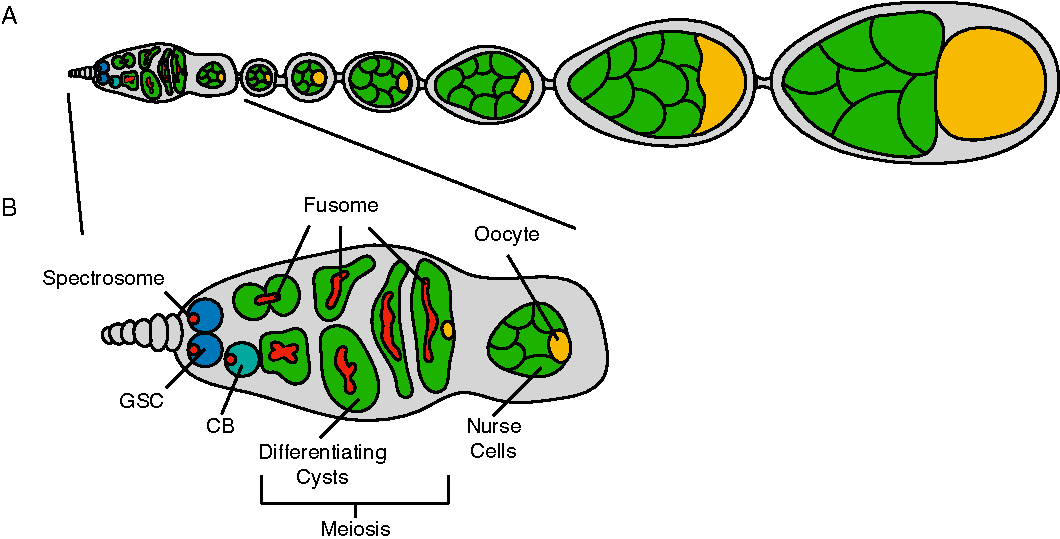
\includegraphics[width=6 in,height=3.046676 in]{./figure/Book Chapter/Figure1} 

}

\caption[\textbf{Schematic of \emph{Drosophila} ovariole.}]{(A) \textbf{Schematic of \emph{Drosophila} ovariole.} \emph{Drosophila} females have two ovaries consisting of 16--20 ovarioles, which are assembly lines for producing mature eggs. The germarium, the structure that houses the germline stem cell (GSC), is present at anterior tip of the ovariole. The germline stem cell asymmetrically divides, giving rise to another GSC and a GSC daughter. The daughter cell then will undergo four incomplete rounds of mitosis, giving rise to a 16-cell cyst. Of the 16 cells one will be specified as the egg while the others serve as polyploid nurse cells that support oocyte and egg development. The surrounding somatic cells encapsulate the 16-cell cyst creating egg chambers. As development proceeds, the nurse cells provide mRNAs and proteins allowing the oocyte to grow in size and to eventually become a mature egg. (B) Inset of a germarium showing the developing germline, with the GSC located at the most anterior tip. Upon differentiation, the CB will undergo 4 incomplete mitotic divisions giving rise to a 16-cell cyst. Only one cell of the sixteen cells completes meiosis and is destined to become the oocyte.}\label{fig:unnamed-chunk-2}
\end{figure}
\hypertarget{alternative-splicing-ensures-accurate-production-of-critical-germline-mrnas-to-regulate-sex-determination-and-differentiation}{%
\section{Alternative splicing ensures accurate production of critical germline mRNAs to regulate sex determination and differentiation}\label{alternative-splicing-ensures-accurate-production-of-critical-germline-mrnas-to-regulate-sex-determination-and-differentiation}}

Splicing decisions are crucial during the generation of mature mRNAs
post-transcriptionally and significantly contribute to germline
development. Splicing is mediated by a large ribonucleoprotein catalytic
complex called the spliceosome, the core of which is made up of five
small nuclear RNAs (snRNA), U1, U2, U4, U5 and U6, that work with
spliceosomal proteins to form a small nuclear ribonucleoprotein complex
(snRNP) ({\textbf{???}}; {\textbf{???}}; {\textbf{???}}; {\textbf{???}}). This
complex removes introns from newly synthesized pre-mRNAs and links
exonic sequences together ({\textbf{???}}). Initially, U1 snRNP recognizes
the donor site, which is located at the 5' end of the intron, and U2
snRNP binds the branch site located at the 3' end, leading to structural
rearrangements of the complex and its associated substrate pre-mRNA
({\textbf{???}}). Catalytic actions of pre-mRNA splicing occur in two
main steps. Cleavage at the 5' splice site forms a lariat-like structure
such that a 2'-5' phosphodiester bond is created between the first
nucleotide of the donor site and a conserved adenosine residue at the
branch site ({\textbf{???}}). Next, a second cleavage event occurs at
the 3' splice site and is followed by ligation of flanking exons to
complete splicing ({\textbf{???}}; {\textbf{???}}).

Alternative splicing is a process by which a single locus can give rise
to many unique mRNA isoforms and their resulting protein variants
({\textbf{???}}). The selection of the splice sites is exquisitely
regulated to determine which exons will be included in the resulting
alternatively spliced transcripts ({\textbf{???}}). Alternative splicing
is highly regulated and is critical to germline development
({\textbf{???}}; {\textbf{???}}). There are a myriad of RNA targets that
must be differentially spliced, and a complex web of interacting
proteins orchestrate production of their splice variants ({\textbf{???}}).
One of the first described instances of alternative splicing in
\emph{Drosophila} females is the splicing of the sex determination gene
\emph{sex-lethal} (\emph{sxl}) ({\textbf{???}}). \emph{sxl} is alternatively spliced to
generate isoforms that control sex determination in somatic tissues
({\textbf{???}}). In females, an autoregulatory loop forms between Sxl
protein, U2AF splicing factor and U1 snRNP ({\textbf{???}}). In
\emph{Drosophila}, the protein component of the U1 and U2 snRNPs are encoded
by a gene called \emph{sans fille} (\emph{snf}) ({\textbf{???}}). Loss of \emph{snf}
results in a sterility phenotype in females that specifically affects
germline \emph{sxl} splicing and leads to a tumor comprised of
undifferentiated cells ({\textbf{???}}; {\textbf{???}}). When
correctly spliced, the resulting Sxl protein recognizes its own
pre-mRNAs by binding both upstream and downstream of Exon 3
({\textbf{???}}). In addition, Sxl protein interacts with the U2AF and
U1 snRNP to block the recognition of splice sites at Exon 3
({\textbf{???}}). As a result, exon 3 is spliced out of the pre-mRNA
in the final transcript that is capable of being translated into a fully
functional protein ({\textbf{???}}). In contrast, males include exon
three in the final \emph{sxl} transcript. Exon 3 contains a premature stop
codon within the \emph{sxl} transcript that results in a truncated protein
that lacks the activity of the female-specific variant ({\textbf{???}}).
Thus, \emph{sxl} is differentially expressed in the male and the female gonad
due to alternative splicing events.

In addition to control of \emph{sxl} via alternative splicing, \emph{sxl}
expression is controlled at the level of transcription by several
transcription factors, such as Ovo ({\textbf{???}}). Ovo is a zinc
finger DNA binding protein that is required in the germline for proper
gametogenesis({\textbf{???}}). \emph{ovo} is also alternatively spliced and
each of its isoforms have different implications for \emph{sxl} expression.
Ovo-A and Ovo-B where the first splice variants of \emph{ovo} shown to be
expressed in the female germline during oogenesis ({\textbf{???}}). In
addition to differences due to alternative exon usage, Ovo-A, unlike
Ovo-B, contains a 381 amino acid N-terminal extension which arises due
to alternative transcription start sites ({\textbf{???}}). Use of
these promoters generates distinct Ova isoforms with unique temporal
requirements during oocyte development; Ovo-B was found to be necessary
and sufficient during early oogenesis and Ovo-A is critical in the later
stages of egg development for a fully functional egg. The \emph{ovo-B} gene
has two characterized isoforms, Ovo+2B and Ovo-2B, which were discovered
through a transposon insertion that disrupts exon splicing of \emph{ovo-B}.
This transposition event prevents inclusion of the exon 2b extension,
producing a nonfunctional protein that accumulates during oogenesis. In
the absence of retrotransposon insertion, the 178-amino acid extension
encoded by exon 2b is included forming a fully functional Ovo protein,
known as Ovo-+2B ({\textbf{???}}). Interestingly, Ovo-B promotes
transcription of \emph{ovarian tumor} (\emph{otu}), which enhances \emph{sxl}
expression (Figure 2) ({\textbf{???}}). The mechanism by which Otu regulates
sxl expression is unknown but various mutations in \emph{otu} lead to a
myriad of phenotypes such as loss of germ cell proliferation, and
inability to complete the differentiation process. The \emph{otu} gene
produces two cytoplasmic protein isoforms, a 104-kDA isoform (Otu-104)
and a 98-kDA isoform (Otu-98) ({\textbf{???}}). Strikingly, only
Otu-104 is capable of rescuing all the \emph{otu} mutant phenotypes,
indicating its requirement during oogenesis, while Otu-98 is dispensable
during this process ({\textbf{???}}). Despite the lack of insight into
how the \emph{otu} splice forms regulate GSC development, its alternative
splicing is critical for oogenesis ({\textbf{???}}). Thus, a cascade of
alternative splicing events regulate production of Sxl in the female
germline to promote oogenesis (Figure 2).

Sxl expression in the female gonad regulates both sex determination as
well as differentiation ({\textbf{???}}). One critical task of Sxl is to
represses Tudor domain containing protein 5-like (\emph{tdrd5l})
({\textbf{???}}). Tdrd5l is present in the cytoplasm of the male
germline, localizing to granules associated with RNA regulation, to
promote male identity and differentiation. Sxl expression the female
gonad represses translation of Tdrd5l to promote female identity
({\textbf{???}}). In addition, female Sxl has been found to regulate
transcription of \emph{PHD finger protein 7 (phf7)}, a key regulator of male
identity ({\textbf{???}}). Sxl was found to recruit SETDB1, a chromatin
writer, to deposit trimethylated H3K9 (H3K9me3) repressing transcription
of \emph{phf7} ({\textbf{???}}). Thus, alternative splicing of \emph{sxl} results
in different sexes helps promote proper sex determination in the
germline (Figure 2). Sxl also fulfills additional functions outside of
sex determination. Sxl is required in the female germline for germline
stem cell GSC differentiation. Loss of Sxl protein causes an
accumulation of single cells and two cell cysts ({\textbf{???}}). It is
thought that Sxl binds \emph{nanos} (\emph{nos}) mRNA, an RNA binding protein that
is necessary for GSC self-renewal, using a canonical Sxl binding
sequence in the 3' UTR ({\textbf{???}}). Loss of Sxl leads to an
accumulation of excess of Nanos protein, which is thought to limit? GSC
differentiation ({\textbf{???}}; {\textbf{???}}; {\textbf{???}}). While
regulation by Sxl is beginning to be deciphered, several aspects remain
to be discovered. For example, Sxl, a splicing factor, is predominantly
cytoplasmic in undifferentiated cells but becomes nuclear as
differentiation proceeds ({\textbf{???}}), yet, how it works as
translational regulator while in the cytoplasm and how it is transported
to the nucleus to function as splicing factor during differentiation are
not known.

Polypyrimidine tract binding proteins (PTBs) promote splicing by binding
polypyrimidine tracts that are \textasciitilde10nt long and bring splice sites
together by means of protein dimerization to promote alternative
splicing ({\textbf{???}}; {\textbf{???}}). A PTB, \emph{half pint}
(\emph{hfp}), a homolog of human PUF60, is important for oogenesis
({\textbf{???}}). Loss of \emph{hfp} results in missplicing of the \emph{otu}
transcripts described above ({\textbf{???}}). In addition, \emph{hfp}
also regulates alternative splicing of \emph{eukaryotic initiation factor 4E}
(\emph{eIF4E}) during development through 3' splice site selection
({\textbf{???}}). Hfp is required to increase the relative abundance of
the longer \emph{eIF4E} transcript ({\textbf{???}}). Lastly, \emph{hfp} also
regulates splicing of \emph{gurken}, a critical regulator of dorsal-ventral
patterning ({\textbf{???}}). Thus, sex determination, differentiation
and production of the determinants of embryonic patterning for the next
generation are all regulated by mechanisms involving alternative
splicing in the female germline.
\begin{figure}

{\centering \includegraphics[width=6.0 in,height=1.483636 in]{./figure/Book Chapter/Figure2} 

}

\caption[\textbf{Schematic of the pathway that promotes alternative splicing of \emph{sxl}.}]{\textbf{Schematic of the pathway that promotes alternative splicing of \emph{sxl} to generate the female \emph{sex determining} variant in the germline.} Ovo-B promotes the transcription of \emph{otu,} which enhances splicing of \emph{sxl}. The female-specific splice form of \emph{sxl} is further enhanced by RNA modification by the m6A writer. Formation of the female-specific form generates a functional Sxl protein. Sxl represses Tdrd5l, a protein that promotes male identify. Additionally, Sxl post-transcriptionally represses \emph{nhp2} to promote cyst formation during differentiation.}\label{fig:unnamed-chunk-3}
\end{figure}
\hypertarget{rna-modifications-direct-splicing-of-sex-determinants-and-translation-of-differentiation-promoting-genes-in-the-germline}{%
\section{RNA modifications direct splicing of sex determinants and translation of differentiation promoting genes in the germline}\label{rna-modifications-direct-splicing-of-sex-determinants-and-translation-of-differentiation-promoting-genes-in-the-germline}}

Post transcriptional RNA modifications are abundant and conserved in all
branches of life ({\textbf{???}}). There have been over 100 described RNA
modifications that can alter stability, function and splicing of RNAs
({\textbf{???}}; {\textbf{???}}). A well-known example of an mRNA
modification is the 5' methylguanosine cap that is added to all mRNAs to
promote their stability and aid in translation initiation
({\textbf{???}}; {\textbf{???}}). A variety of RNA modifications have
been linked to developmental transitions, such as those affecting GSC
fate ({\textbf{???}}; {\textbf{???}}). Specifically during oogenesis,
N6A-methyladenosine (m\textsuperscript{6}A) has been shown to be important for
differentiation of germline stem cell daughter cells in females by
ensuring proper female-specific splicing of \emph{sxl} ({\textbf{???}}).
Additionally, the H/ACA box complex, an RNP complex responsible for
depositing pseudouridine on rRNA, has been suggested to be regulated by
Sxl during the germline stem cell to daughter cell transition and is
required for proper cyst differentiation ({\textbf{???}}; {\textbf{???}}).

m\textsuperscript{6}A is prevalent on mRNA and is mediated by a methyltransferase
complex that deposits a methyl-group at the sixth nitrogen on adenosine
({\textbf{???}}). In \emph{Drosophila,} m\textsuperscript{6}A is placed by a m\textsuperscript{6}A writer
complex consisting of Xio, Virilizer (Vir), Spenito (Nito), female
lethal d (fl(2)d), Methyltransferase like 3 (Mettl3) and
Methyltransferase like 14 (Mettl14) ({\textbf{???}}). Some described roles
of m\textsuperscript{6}A involve modulating RNA-structure, facilitating mRNA
degradation, promoting translation initiation and mediating alternative
splicing ({\textbf{???}}). Interestingly, the m\textsuperscript{6}A writer complex
has been linked to \emph{sxl} splicing during \emph{Drosophila} oogenesis
({\textbf{???}}). miCLIP data revealed that m\textsuperscript{6}A must be placed at
intergenic regions of the \emph{sxl} mRNA in order to produce the
female-specific isoform ({\textbf{???}}). Accordingly. loss of m\textsuperscript{6}A
complex members such as \emph{spenito} result in expression of the male
specific isoform of \emph{sxl}, and tumors of undifferentiated cells, similar
to loss of \emph{sxl} ({\textbf{???}}); ({\textbf{???}}). This suggests that
m\textsuperscript{6}A enables proper splicing of female-specific \emph{sxl}, which allows for
proper differentiation of germline stem cells into cystoblast daughter
cells (Figure 2).

Pseudouridine is one of the most abundant RNA modifications
({\textbf{???}}). Although most commonly found on tRNAs, pseudouridine is
also found on mRNAs as well as rRNA ({\textbf{???}}). Unlike the
canonical nucleoside uridine which is attached to the sugar via a
nitrogen-carbon bond, pseudouridine is a uridine isomer attached through
a carbon-carbon bond ({\textbf{???}}). Pseudouridine can be placed by two
different classes of enzymes; either by a sequence specific
pseudouridine synthase or a small RNA guided complex called the box
H/ACA ribonucleoprotein ({\textbf{???}}). Depletion of the H/ACA box
complex member Nucleolar Protein Family A Member 2 (NHP2) in the
germline leads to an accumulation of 4- and 8- cell cysts that do not
transition to the 16-cell cyst stage ({\textbf{???}}). Interestingly,
the accumulation of single cells due to loss of \emph{sxl} is partially
rescued by loss of \emph{NHP2 indicating that this sxl phenotype is due to
excess NHP2} ({\textbf{???}}). Consistent with this notion, Sxl
interacts with \emph{nhp2} mRNA suggesting that Sxl may impose a regulatory
function, in this case likely repression of \emph{nhp2} to allow initiation
of the differentiation program (Figure 2) ({\textbf{???}}). Thus,
although it is clear that RNA modifications help to ensure proper
splicing of sex determination factors, but the pathway, mechanism, and
direct targets remain unresolved.

\hypertarget{production-of-ribosomes-is-finely-tuned-to-facilitate-differentiation}{%
\section{Production of ribosomes is finely tuned to facilitate differentiation}\label{production-of-ribosomes-is-finely-tuned-to-facilitate-differentiation}}

While splicing mediates proper mRNA production, access of the mature
mRNAs to ribosomes controls their translation. Once mRNAs are gated for
translation, proper ribosome levels control protein production. The
levels of ribosomes during early oogenesis are strictly regulated and
shockingly dynamic. Ribosome biogenesis is the process of transcribing
and processing the ribosomal RNA (rRNA) components, as well as
transcribing and translating the protein constituents of the ribosome
({\textbf{???}}; {\textbf{???}}; {\textbf{???}}; {\textbf{???}}). This
process is exquisitely regulated as ribosome biogenesis is one of the
most energy intensive tasks of maintaining cell homeostasis and is even
more crucial in proliferative cells ({\textbf{???}}). In addition to
the high energy requirement of ribosome biogenesis, all of the
components of the ribosome must be coordinated in their production. The
process of ribosome biogenesis involves a series of coordinated steps of
processing and assembly that involve dozens of non-coding RNAs and
proteins and the molecular details of this process have been thoroughly
covered in detail in several recent reviews ({\textbf{???}}; {\textbf{???}}; {\textbf{???}}). Briefly, ribosomal DNA (rDNA) is present in
multicopy stretches within the genome; these areas of DNA are localized
to a subnuclear organelle called the nucleolus ({\textbf{???}}; {\textbf{???}}; {\textbf{???}}). rDNA is transcribed into rRNA in
the nucleolus and processing steps begin cotranscriptionally
({\textbf{???}}) to remove internal and external spacers found in immature
rRNA ({\textbf{???}}; {\textbf{???}}; {\textbf{???}}; {\textbf{???}}). As these processing steps occur, the rRNA is
covalently modified and ribosomal proteins begin to interact with the
partially processed rRNA ({\textbf{???}}; {\textbf{???}}; {\textbf{???}}; {\textbf{???}}; {\textbf{???}}). When the rRNA is mostly
mature it is exported from the nucleus to the cytoplasm where the small
and large subunits of the ribosome fully mature and assemble
({\textbf{???}}; {\textbf{???}}; {\textbf{???}}; {\textbf{???}}; {\textbf{???}}). Errors at any of these steps can result in ribosome
biogenesis defects which in humans result in disease states known as
ribosomopathies ({\textbf{???}}; {\textbf{???}}; {\textbf{???}}; {\textbf{???}}; {\textbf{???}}; {\textbf{???}}).

Curiously, despite the presence of ribosomes across cell types and
sharing similar molecular origins, ribosomopathies manifest as tissue
specific defects rather than pleiotropic phenotypes ({\textbf{???}}; {\textbf{???}}; {\textbf{???}}; {\textbf{???}}; {\textbf{???}}).
The reasons behind the unique, tissue-specific manifestations are still
being investigated but in several cases it seems that stem cells may be
particularly sensitive to perturbations in ribosome biogenesis
({\textbf{???}}; {\textbf{???}}; {\textbf{???}}; {\textbf{???}}). Indeed, a growing body of evidence is beginning
to suggest that \emph{Drosophila} GSCs not only have a specific requirement
for ribosome biogenesis, but also that ribosome biogenesis, as well as
global translation, vary greatly over the course of GSC differentiation
and are uncoupled during early oogenesis ({\textbf{???}}; {\textbf{???}}). These attributes make \emph{Drosophila} oogenesis an
excellent system to address how perturbations of ribosome levels affects
stem cell differentiation.

In order to maintain stem cell fate, GSCs asymmetrically partition
factors required for ribosome biogenesis by retaining more of this
machinery than they pass on to daughter cells ({\textbf{???}}; {\textbf{???}}). In particular, Underdeveloped (Udd), an rRNA
transcription factor segregates asymmetrically to the GSC during mitosis
and seems to promote a high rate of rRNA synthesis within the GSC
({\textbf{???}}). Furthermore, Wicked (Wcd), a U3 snoRNP complex member
required for rRNA maturation, is also asymmetrically partitioned to GSCs
and associates with the original spectrosome, an ER rich organelle found
in GSCs and CBs ({\textbf{???}}), of the dividing GSC. How GSCs
carry out this specialized cellular division requires further
investigation, however, asymmetric stem cell division is crucial for
proper differentiation ({\textbf{???}}; {\textbf{???}}; {\textbf{???}}).Consistent with this loss of \emph{wcd} results in premature
differentiation of GSCs ({\textbf{???}}). Nascent rRNA production,
measured by BrUTP incorporation, and presumably ribosomes, are produced
at high levels in GSCs but this production drops in CBs and in
subsequent stages (Figure 3) ({\textbf{???}}). Additionally, it has been
observed that certain ribosome biogenesis components are expressed at
high levels specifically in the germline ({\textbf{???}}). In particular,
RNA exonuclease 5 (Rexo5) is an RNA exonuclease that facilitates
ribosome biogenesis by trimming snoRNAs as well as rRNAs
({\textbf{???}}). Depletion of \emph{rexo5} in the germline results in
an accumulation of egg chambers that bud off from the germarium, but do
not grow in size, and causes defects in GSC proliferation
({\textbf{???}}). These observations suggest that the machinery for
ribosome biogenesis is not only critical for germline development but is
also dynamically regulated.

Sanchez et al.~demonstrated that the dynamic nature of rRNA
transcription during germline development is not simply a consequence of
the differentiation process. Instead, lowering ribosome biogenesis is
required for timely differentiation, but severe loss of ribosome
biogenesis causes formation of stem-cysts, a product of perturbed
cytokinesis of GSC daughters ({\textbf{???}}; {\textbf{???}}; {\textbf{???}}) . Somewhat surprisingly, despite their increased
retention of ribosome biogenesis components, GSCs exhibit a lower rate
of translation compared to daughter cells and cyst stages (Figure 3).
This finding invokes the hypothesis that despite the GSCs elevated
capacity for ribosome biogenesis, GSCs do not intrinsically require
higher ribosome levels for translation. Instead, the data is suggestive
of the possibility that GSCs produce high levels of ribosomes in order
to pass them on to and facilitate differentiation of their daughter
cells. We thus hypothesize that a ribosome biogenesis checkpoint could
couple ribosome production to cell cycle progression to ensure a
sufficient ribosome concentration is passed from the GSC to the daughter
CB. Conversely, increasing ribosome biogenesis via overexpression of
TIF-IA, an RNA Pol I transcription initiation factor that is required
for rRNA synthesis ({\textbf{???}}), results in a failure of germ cells
to differentiate, causing a marked overproliferation of undifferentiated
GSC daughters ({\textbf{???}}). This overproliferation may be caused by
bypassing or rapid progression through the proposed ribosome biogenesis
checkpoint such that the cell cycle is hastened in response to elevated
ribosome biogenesis. The overproliferation of undifferentiated germ
cells when ribosome levels are elevated is consistent with observations
that high ribosome levels lead to rapidly growing cancers
({\textbf{???}}; {\textbf{???}}; {\textbf{???}}).

Although reducing ribosome biogenesis tends to result in the formation
of a stem-cyst as previously described, some factors that play a role in
ribosome biogenesis have a less severe phenotypes. For example, some
mutants of the ribosomal protein S2 (rps2) gene have a repeating
egg-chamber mid-oogenesis defect, wherein ovarian development halts at
stage 5 and successive egg chambers do not grow in size and eventually
die, resulting in sterility ({\textbf{???}}). This phenotype may be
the consequence of incomplete loss of function as the allele that
results in the repeating egg chamber phenotype reduces mRNA expression
of \emph{rps2}, incompletely, by 60-70\%, while other allelic combinations
result in embryonic lethality ({\textbf{???}}). Incomplete loss of
function alleles for another ribosomal protein, \emph{ribosomal protein S3},
result in a similar repeating egg chamber phenotype
{[}Sæbøe-Larssen1998{]}. These observations suggest that partial loss of
ribosome biogenesis during oogenesis may be tolerated during
differentiation but results in phenotypes at a later phase of egg
production, consistent with the model that high levels of biogenesis in
early stages supply the ribosomes for subsequent differentiation and
development.

Not only do ribosome levels vary but a class of ribosomal protein
paralogs are enriched specifically in early germ cells ({\textbf{???}}).
Several variant ribosomal proteins such as \emph{ribosomal proteins S5b}
(\emph{rps5b}), \emph{s10a}, \emph{s19b}, and \emph{l22}-like are enriched in the germline
and others are enriched during early oogenesis ({\textbf{???}}). The role
of these ribosomal proteins has not been thoroughly explored, but their
presence indicates either a role for specialized ribosomes early during
germline development or as a way to further increase the availability of
ribosomal proteins to facilitate the high level of ribosome production
in GSCs. One of these ribosomal protein paralogs, RpS5b, has recently
been characterized ({\textbf{???}}). \emph{rps5b} is most highly expressed in
ovaries in contrast to its paralog, \emph{ribosomal protein S5a} (\emph{rps5a}),
which is expressed at high levels ubiquitously ({\textbf{???}}). Loss of
\emph{rps5a} in the germline does not cause a germline phenotype, however,
loss of \emph{rps5b} results in a mid-oogenesis defect that is further
exacerbated when \emph{rps5a} is depleted in a \emph{rps5b} mutant background
({\textbf{???}}). This could suggest that RpS5a and RpS5b are functionally
similar and that the RpS5b phenotype results from lowering the overall
amount of RpS5 available during oogenesis. However, RpS5b was also found
to interact preferentially with mRNAs that encode proteins involved in
mitochondrial electron transport, in contrast to RpS5a which binds mRNAs
from a broad spectrum of gene categories ({\textbf{???}}). In accordance
with the binding data, \emph{rps5b} depleted ovaries expressed lower levels
of proteins involved in oxidative phosphorylation and mitochondrial
respiration ({\textbf{???}}). This evidence suggests that the expression
of ribosomal protein paralogs may be a part of specialized ribosomes
that translate specific groups of mRNAs; however, these ribosomal
protein paralogs must be carefully analyzed to determine if they make up
bonafide special ribosomes or instead have ribosome independent
functions ({\textbf{???}}).

What regulates ribosome biogenesis to allow for it to be dynamic during
early \emph{Drosophila} germline development? The best understood regulator
of ribosome biogenesis is the Target of Rapamycin (TOR) pathway
({\textbf{???}}; {\textbf{???}}; {\textbf{???}}; {\textbf{???}})
TOR is a kinase that is part of two distinct subcomplexes, TOR complex 1
(TORC1) and TOR complex 2 (TORC2) ({\textbf{???}}). These
complexes have distinct biological roles. TORC2 has been shown to
function as an important regulator of the cytoskeleton
({\textbf{???}}). Whereas, TORC1 receives and integrates several
different signals including nutritional and growth factors and its
activity promotes pro-proliferative activities such as global
translation, ribosomal protein translation, and cell cycle progression
({\textbf{???}}; {\textbf{???}}; {\textbf{???}}). TORC1 activity also helps
to coordinate the transcription and translation of the components
required for ribosome biogenesis ({\textbf{???}}; {\textbf{???}}; {\textbf{???}}). In \emph{Drosophila,} TORC1 activity is high in GSCs through
the 4-cell cyst, but TORC1 activity dips in 8 and 16 cell cysts and
subsequently increases after the cyst stages ({\textbf{???}}).
Interestingly, the landscape of TORC1 activity resembles the landscape
of ribosome biogenesis, but not global translation (Figure 3)
({\textbf{???}}; {\textbf{???}}). However, loss of TORC1 components does
not phenocopy perturbation of ribosome biogenesis ({\textbf{???}}).
This is possibly because TORC1 plays a broader role in early oogenesis
given the myriad of regulatory functions TORC1 is known to play in other
systems ({\textbf{???}}; {\textbf{???}}; {\textbf{???}}; {\textbf{???}}; {\textbf{???}}). A downstream effector of mTORC1, La related protein 1
(Larp1) is known to silence ribosomal protein translation in mammals
through binding to terminal oligopyrimidine tracts in the 5'UTR of its
targets ({\textbf{???}}; {\textbf{???}}; {\textbf{???}}; {\textbf{???}}); however, the same has yet to be
demonstrated for the \emph{Drosophila} ortholog, La related protein (Larp).
Tantalizingly, Larp is required for male and female fertility in
\emph{Drosophila}, but details of Larp's precise role in the female and
oogenesis are lacking ({\textbf{???}}; {\textbf{???}}). In contrast,
in males Larp is required for proper spindle pole formation as well as
proper cytokinesis ({\textbf{???}}). Given the regulatory role Larp
plays in ribosome biogenesis in mammals and the data from \emph{Drosophila}
spermatogenesis, Larp could facilitate the dynamic nature of ribosome
biogenesis during GSC differentiation and meiosis. However, further
study is required to understand the role of Larp during GSC
differentiation and oogenesis to determine its function in this context.

The process of differentiation requires major cellular reprogramming.
Surprisingly, despite being required for cell viability ribosome
biogenesis and global translation are two key programs that are
modulated to shape GSC differentiation({\textbf{???}}; {\textbf{???}}).
When ribosome production is improperly modulated during GSC
differentiation it results in characteristic phenotypes, accumulation of
single cells if biogenesis components are overexpressed and formation of
a stem-like cyst if ribosome biogenesis components are knocked down in
the germline ({\textbf{???}}; {\textbf{???}}). Additionally, several
ribosomal protein variants are highly enriched in ovaries and they may
perform special functions, however, these variants are just beginning to
be studied. Additionally, based on what we know of the mechanisms and
networks that control ribosome biogenesis in \emph{Drosophila} oocytes, the
dynamic nature of ribosome biogenesis seems likely to be conserved;
however, further investigation is required to determine and compare the
basis of ribosome biogenesis control.
\begin{figure}

{\centering \includegraphics[width=4.536585 in,height=6 in]{./figure/Book Chapter/Figure3} 

}

\caption[\textbf{Global translation rate, rRNA transcription rate, and mTorc1 activity during development.}]{\textbf{Global translation rate, rRNA transcription rate, and mTorc1 activity during development.} Schematic representing the germarium and plots representing relative changes in global translation rate, rRNA transcription rate, and mTorc1 activity during development at the developmental stages indicated. As germline stem cell differentiation occurs rRNA production decreases, while global translation initially increases as differentiation occurs then falls off post differentiation. A global regulator of both translation and rRNA production, mTorc1 activity decreases during differentiation and increases post differentiation.}\label{fig:unnamed-chunk-4}
\end{figure}
\hypertarget{hand-off-mechanisms-facilitated-by-combinatorial-rna-binding-proteins-dynamically-shape-the-translational-landscape-during-oogenesis}{%
\section{Hand off mechanisms facilitated by combinatorial RNA binding proteins dynamically shape the translational landscape during oogenesis}\label{hand-off-mechanisms-facilitated-by-combinatorial-rna-binding-proteins-dynamically-shape-the-translational-landscape-during-oogenesis}}

While some mRNAs are translated post-transcriptionally, other critical
mRNAs are translationally regulated. For efficient translation of mRNAs,
it is thought that the mRNAs must be circularized - bringing their 5'
cap and 3' poly A tail in close proximity to each other ({\textbf{???}}; {\textbf{???}}; {\textbf{???}}). This interaction is mediated by cap
binding proteins such as eukaryotic initiation factor 4E (eIF4E) and the
poly-A binding protein (PABP)({\textbf{???}}; {\textbf{???}}; {\textbf{???}}; {\textbf{???}}). A longer poly-A tail and uninhibited
access to the 5' cap for eIF4E is believed to promote efficient
translation ({\textbf{???}}). A major mode of translational
regulation is that RNA binding proteins (RBPs) recognize cognate
sequences in the 3' UTRs of their target mRNAs ({\textbf{???}}). The
binding of the RBP prevents circularization of the mRNA and inhibits
efficient translation initiation, leading to reduced translation
({\textbf{???}}). RBP binding to the 3' UTR can mediate translation
inhibition by recruiting cofactors to inhibit circularization
({\textbf{???}}).This inhibition of circularization can be achieved by
RBP binding to the cap and competing with eIF4E, removal of the cap by
the decapping machinery, or recruitment of factors such as the CCR4-Not
complex to shorten poly-A tail length ({\textbf{???}}). In some
cases, RBPs can both block initiation as well as mediate shortening of
the poly-A tail ({\textbf{???}}).

As mentioned in the germline several developmental processes such as
stem cell maintenance, differentiation, mitosis and meiosis are
coordinated and successful transition through these diverse programs
relies on precise translational control (Figure 4) ({\textbf{???}}; {\textbf{???}}). As factors that interfere with translation such as
the decapping machinery and the poly-A tail shortening CCR4-Not complex
are expressed continuously during oogenesis, and cannot support dynamic
translational control on their own, a dynamic and diverse landscape of
translational regulators has evolved to allow for fine-scale temporal
control of mRNA translation ({\textbf{???}}; {\textbf{???}}). To add an
additional layer of complexity, the expression or abundance of several
RBPs that regulate translational control oscillate as oogenesis
progresses (Figure 4) ({\textbf{???}}; {\textbf{???}}; {\textbf{???}}). As
the levels of RBPs decrease, their bound mRNA targets are licensed for
translation ({\textbf{???}}; {\textbf{???}}; {\textbf{???}}). There are three
major themes that work to control mRNA translation: 1. RBPs collaborate
in a combinatorial manner to regulate mRNAs, 2. Target mRNAs are handed
off from one RBP complex to another as levels oscillate during oogenesis
to consistently repress or promote target mRNA translation, and 3.
Multiple feedback mechanisms operate to mediate each transition (Figure
4) ({\textbf{???}}). The feedback mechanism has been extensively
reviewed elsewhere and is not the focus of this chapter ({\textbf{???}}; {\textbf{???}}). Here, we outline how RBPs both collaborate as well
hand off mRNAs during the transition from GSC to mature oocyte.

GSCs rely on several factors to maintain self-renewal, two of the main
factors are Pumilio (Pum) and Nanos (Nos), which work in a combinatorial
fashion to repress the translation of differentiation-promoting mRNAs
(Figure 4) ({\textbf{???}}; {\textbf{???}}; {\textbf{???}}; {\textbf{???}}).
Pum, a member of the conserved Pum- and Fem-3-binding factor (PUF)
family of proteins, is present at high levels in the undifferentiated
germline cells of the ovary, including GSCs, CBs, and
early-differentiating cysts ({\textbf{???}}; {\textbf{???}}). Independent of
other factors, Pum can directly bind mRNA, but it requires the catalytic
activity of other proteins to regulate translation of its targets in the
\emph{Drosophila} germline ({\textbf{???}}; {\textbf{???}}). Pum is known
to have dynamic interactions with two critical regulators, Nos in GSCs,
and Brain tumor (Brat) in CBs (Figure 4) ({\textbf{???}}; {\textbf{???}}; {\textbf{???}}; {\textbf{???}}; {\textbf{???}}; {\textbf{???}}). Nos, a well conserved RNA binding protein, has the
ability to bind mRNA, albeit at low affinity and requires the presence
of Pum to recognize its targets ({\textbf{???}}). Nanos directly
interacts with Not1, a member of the CCR4-Not complex, recruiting it to
target mRNAs, such as \emph{meiotic P26} (\emph{mei-p26}) and \emph{brat}, to regulate
their translation ({\textbf{???}}; {\textbf{???}}; {\textbf{???}}).
While in some systems Pum can directly recruit the CCR4-Not complex,
activity of \emph{nos} is required for this interaction in the \emph{Drosophila}
germline ({\textbf{???}}; {\textbf{???}}). Upon loss of Pum, Nanos or Twin,
GSCs fail to maintain stem cell fate and differentiate into stem cell
daughters, resulting in the inability to sustain oogenesis as outlined
below.

An example of distinct, stage-specific translational control by
Pum/Nos/CCR4-Not complex in the germline is the mechanism by which
\emph{polar granule component} (\emph{pgc}), a germline-specific transcriptional
repressor, is controlled (Figure 4) ({\textbf{???}}). Pgc interacts with
the Positive Transcription Elongation Factor (P-TEFb) complex and
inhibits the phosphorylation of the Serine-2 residue that is critical
for transcriptional elongation, resulting in global transcriptional
silencing ({\textbf{???}}). A single pulse of expression of Pgc
protein in the CB allows for epigenetic and transcriptomic reprogramming
during differentiation ({\textbf{???}}). While \emph{pgc} mRNA is expressed
highly and ubiquitously throughout oogenesis, translation of \emph{pgc} mRNA
is tightly regulated to mitigate the effects of its potent
transcriptional silencing activity. The \emph{pgc} 3' UTR contains a
conserved consensus sequence that is transiently and sequentially bound
by multiple distinct, developmentally regulated RBPs ({\textbf{???}}).
This 3' UTR sequence is required for post-transcriptional control of
\emph{pgc} as Pgc protein expression is restricted to the CB. In the GSCs,
Pum and Nos bind the \emph{pgc} 3' UTR and recruit Twin a component of the
CCR4-Not complex to deadenylate \emph{pgc} mRNA and inhibit its translation
(Figure 4) ({\textbf{???}}). In addition to \emph{pgc}, Pum/Nos and Twin also
regulate Brain tumor (Brat) ({\textbf{???}}). Brat is a TRIM-NHL domain
protein expressed in the germline that represses translation by engaging
with d4EHP and competing with the cap-binding protein eIF4E to prevent
translation initiation (Figure 4) ({\textbf{???}}; {\textbf{???}}; {\textbf{???}}). While \emph{brat} mRNA is expressed in the GSC, it is
specifically repressed by Nos and Pum . In addition to these targets,
several differentiation promoting mRNAs such as \emph{meiP26} are also
repressed ({\textbf{???}}). Thus, in the GSCs, a combination of Pum, Nos
and CCR4-Not complex are required for repressing translation of several
critical differentiation promoting mRNAs ({\textbf{???}}; {\textbf{???}}; {\textbf{???}}; {\textbf{???}}).

Subsequent differentiation of the GSC daughters relies on several
factors to repress expression of \emph{nos} mRNA ({\textbf{???}}; {\textbf{???}}). Differentiation is initiated upon Bam expression in the
CB, where Bam and its binding partner benign gonial cell neoplasm (Bgcn)
act through a sequence in the \emph{nos} 3' UTR to its inhibit translation
(Figure 4) ({\textbf{???}}; {\textbf{???}}). This repression mechanism
includes deadenylation activity by Twin, which works in conjunction with
Bam and Bgcn ({\textbf{???}}). As Nos protein levels decrease in the CB,
\emph{pgc} and \emph{brat} mRNAs are translated ({\textbf{???}}). The expressed
Brat protein now partners with Pum to repress translation of GSC
self-renewal genes (Figure 4) ({\textbf{???}}). In addition, expression
of Mei-P26 increases initiating interactions with Bam, Bgcn and Sxl.
Mei-P26 then promotes translational repression of GSC fate promoting
genes such as \emph{nos}, allowing for further differentiation by cooperating
with Bam and Bgcn ({\textbf{???}}; {\textbf{???}}). As the CB
differentiates into 2-, 4-, 8- and 16- cell cysts, levels of Nanos
protein rebound. However, in spite of the presence of Nos, Pum partners
with Brat to suppress \emph{pgc} translation in the 4- to 16-cell cyst stages
(Figure 4) ({\textbf{???}}). Thus, in CBs, absence of Nos allows for Pum
to complex with a different subset of proteins as well as license
expression of new translational regulators to promote differentiation.

After cyst differentiation, Pum protein levels decrease and expression
of another translational repressor, Bruno (Bru), increases
({\textbf{???}}; {\textbf{???}}; {\textbf{???}}; {\textbf{???}}). Downregulation of Pum expression is
critical for the transition from GSC to an oocyte
({\textbf{???}}; {\textbf{???}}). Rbfox1, an RBP whose
cytoplasmic isoform regulates the translation of specific mRNAs in the
germline is responsible for repressing Pum translation through binding
of a consensus sequence in the \emph{pum} 3' UTR (Figure 4)
({\textbf{???}}). Loss of Rbfox1 leads to an expansion of Pum
protein expression and a disruption of differentiation
({\textbf{???}}). Repression of Pum levels by Rbfox1 allows
for Bru expression ({\textbf{???}}). Surprisingly, Bru can
bind to a sequence in the 3' UTR that is very similar to Pum binding
sequence (Figure 4)({\textbf{???}}). Bruno blocks translation
initiation by interacting with Cup, a conserved eIF4E binding protein
({\textbf{???}}; {\textbf{???}}). In fact, Bru binds the same sequence in
the \emph{pgc} 3' UTR as Nos/Pum to prevent \emph{pgc} translation
({\textbf{???}}). This mode of translation repression is not restricted
to \emph{pgc}, rather a cohort of maternal mRNAs are co-regulated by Pum and
Bru representing a hand-off mechanism for repression of maternal mRNAs
({\textbf{???}}).
\begin{figure}

{\centering \includegraphics[width=5 in,height=6.157635 in]{./figure/Book Chapter/Figure4} 

}

\caption[\textbf{Schematic of combinatorial and dynamic translation regulation in the \emph{Drosophila} germarium.}]{\textbf{Schematic of combinatorial and dynamic translation regulation in the \emph{Drosophila} germarium.} In the GSCs Nos, Pum and Twin form a complex to inhibit the translation of differentiation mRNAs such as \emph{pgc}, which increases throughout oogenesis. Expression of Bam in the CB initiates differentiation by interacting with its partner Bgcn and Mei-P26 to repress the translation of GSC-expressed mRNAs, specifically \emph{nos}. As Nos protein levels decrease in the CB, Pum is available to partner with Brat to repress the translation of self-renewal genes and \emph{pgc}. In cyst stages, Rbfox1 binds the \emph{pum} 3' UTR to inhibit its translation. Throughout oogenesis Bru and Cup continuously block translation of \emph{pgc}.}\label{fig:unnamed-chunk-5}
\end{figure}
\hypertarget{summary}{%
\section{Summary}\label{summary}}

Decades of work using elegant genetics has revealed several paradigms in
which splicing machinery, RNA modifying enzymes, ribosome levels, and
translational regulation mediates the transition from GSC to oocyte
fate. However, several critical details such as the direct targets and
mechanisms still need to be deciphered. Together the advent of
cost-effective sequencing technologies combined with the increasing
ability to easily create mutants in previously uncharacterized genes
will allow us to further elucidate the regulatory logic (underlying or
of) this critical transition.

\setstretch{1.0}

\setstretch{1.0}

























































\hypertarget{a-translation-control-module-coordinates-germline-stem-cell-differentiation-with-ribosome-biogenesis-during-drosophila-oogenesis}{%
\chapter{\texorpdfstring{A translation control module coordinates germline stem cell differentiation with ribosome biogenesis during \emph{Drosophila} oogenesis}{A translation control module coordinates germline stem cell differentiation with ribosome biogenesis during Drosophila oogenesis}}\label{a-translation-control-module-coordinates-germline-stem-cell-differentiation-with-ribosome-biogenesis-during-drosophila-oogenesis}}

Elliot T. Martin\textsuperscript{1}*, Patrick Blatt\textsuperscript{1}*, Elaine Nguyen\textsuperscript{2}, Roni Lahr\textsuperscript{2}, Sangeetha Selvam\textsuperscript{1}, Hyun Ah M. Yoon\textsuperscript{1,3}, Tyler Pocchiari\textsuperscript{1,4}, Shamsi Emtenani\textsuperscript{5}, Daria E. Siekhaus\textsuperscript{5}, Andrea Berman\textsuperscript{2}, Gabriele Fuchs\textsuperscript{1†} and Prashanth Rangan\textsuperscript{1†}

\textsuperscript{1}Department of Biological Sciences/RNA Institute, University at Albany SUNY, Albany, NY 12202

\textsuperscript{2}Department of Biological Sciences, University of Pittsburgh, Pittsburgh, PA 15260

\textsuperscript{3}Albany Medical College, Albany, NY 12208

\textsuperscript{4}SUNY Upstate Medical University, Syracuse, NY 13210-2375

\textsuperscript{5}Institute of Science and Technology Austria, Klosterneuburg, Austria

*These authors contributed equally to this work

\textsuperscript{†}Co-corresponding authors

Email: gfuchs@albany.edu, prangan@albany.edu

\setstretch{2.0}

\hypertarget{summary-1}{%
\section{Summary:}\label{summary-1}}

Ribosomal defects perturb stem cell differentiation, causing ribosomopathies. How ribosome levels control stem cell differentiation is not fully known. Here we discovered that three RNA helicases govern ribosome biogenesis and \emph{Drosophila} oogenesis. Loss of these helicases, which we named Aramis, Athos and Porthos, aberrantly stabilized p53, arrested the cell cycle and stalled GSC differentiation. Aramis controls cell cycle progression by regulating translation of mRNAs containing a Terminal Oligo Pyrimidine (TOP) motif in their 5'-UTRs; we find TOP motifs confer sensitivity to ribosome levels mediated by La-related protein (Larp). One such TOP-containing mRNA codes for {No}vel {N}ucleolar protein 1 (Non1), a conserved p53 destabilizing protein. Upon a sufficient ribosome concentration, Non1 is expressed and promotes GSC cell cycle progression via p53 degradation. Thus, a previously unappreciated TOP-motif in \emph{Drosophila} responds to reduced ribosome biogenesis to co-regulate the translation of ribosomal proteins and a p53 repressor, coupling ribosome biogenesis to GSC differentiation.

\hypertarget{introduction-1}{%
\section{Introduction}\label{introduction-1}}

All life depends on the ability of ribosomes to translate mRNAs into proteins. Despite this universal requirement, perturbations in ribosome biogenesis affects some cell types more than others. Stem cells, the unique cell type that underlies the generation and expansion of tissues, in particular have an increased ribosomal requirement ({\textbf{???}}; {\textbf{???}}; {\textbf{???}}; {\textbf{???}}; {\textbf{???}}). Ribosome production and levels are dynamically regulated to maintain higher amounts in stem cells ({\textbf{???}}; {\textbf{???}}; {\textbf{???}}; {\textbf{???}}; {\textbf{???}}; {\textbf{???}}). For example, ribosome biogenesis components are often differentially expressed, as observed during the differentiation of embryonic stem cells, osteoblasts, and myotubes ({\textbf{???}}; {\textbf{???}}; {\textbf{???}}). In some cases, such as during \emph{Drosophila} germline stem cell (GSC) division, ribosome biogenesis factors asymmetrically segregate during asymmetric cell division, such that a higher pool of ribosome biogenesis factors is maintained in the stem cell compared to the daughter cell ({\textbf{???}}; {\textbf{???}}; Blatt, Martin, Breznak, \& Rangan, 2020). Reduction of ribosome levels in several stem cell systems can cause differentiation defects ({\textbf{???}}; {\textbf{???}}; {\textbf{???}}; {\textbf{???}}). In \emph{Drosophila,} perturbations that reduce ribosome levels in the GSCs result in differentiation defects causing infertility ({\textbf{???}}). Similarly, humans with reduced ribosome levels are afflicted with clinically distinct diseases known as ribosomopathies, such as Diamond-Blackfan anemia, that often result from loss of proper differentiation of tissue-specific progenitor cells ({\textbf{???}}; {\textbf{???}}; {\textbf{???}}; {\textbf{???}}; {\textbf{???}}; {\textbf{???}}). However, the mechanisms by which ribosome biogenesis is coupled to proper stem cell differentiation remain incompletely understood.

Ribosome production requires the transcription of ribosomal RNAs (rRNAs) and of mRNAs encoding ribosomal proteins ({\textbf{???}}; {\textbf{???}}; {\textbf{???}}; {\textbf{???}}; {\textbf{???}}; {\textbf{???}}). Hundreds of factors including helicases and endonucleases, transiently associate with maturing rRNAs to facilitate rRNA processing, modification, and folding ({\textbf{???}}; {\textbf{???}}; {\textbf{???}}; {\textbf{???}}). Ribosomal proteins are imported into the nucleus, where they assemble with rRNAs to form precursors to the 40S and 60S ribosomal subunits, which are then exported to the cytoplasm ({\textbf{???}}; {\textbf{???}}; {\textbf{???}}; {\textbf{???}}; {\textbf{???}}; {\textbf{???}}; {\textbf{???}}; {\textbf{???}}). Loss of RNA Polymerase I transcription factors, helicases, exonucleases, large or small subunit ribosomal proteins, or other processing factors all compromise ribosome biogenesis and trigger diverse stem cell-related phenotypes ({\textbf{???}}; {\textbf{???}}; {\textbf{???}}; {\textbf{???}}; {\textbf{???}}).

Nutrient availability influences the demand for \emph{de novo} protein synthesis and thus ribosome biogenesis ({\textbf{???}}; {\textbf{???}}; {\textbf{???}}; {\textbf{???}}). In mammals, mRNAs that encode the ribosomal proteins contain a Terminal Oligo Pyrimidine (TOP) motif within their 5' untranslated region (UTR), which regulates their translation in response to nutrient levels ({\textbf{???}}; {\textbf{???}}; {\textbf{???}}; {\textbf{???}}). Under growth-limiting conditions, La related protein 1 (Larp1) binds to the TOP sequences and to mRNA caps to inhibit translation of ribosomal proteins ({\textbf{???}}; {\textbf{???}}; {\textbf{???}}; {\textbf{???}}). When growth conditions are suitable, Larp1 is phosphorylated by the nutrient/redox/energy sensor mammalian Target of rapamycin (mTOR) complex 1 (mTORC1), and does not efficiently bind the TOP sequence, thus allowing for translation of ribosomal proteins ({\textbf{???}}; {\textbf{???}}; {\textbf{???}}; {\textbf{???}}). In some instances, Larp1 binding can also stabilize TOP-containing mRNAs ({\textbf{???}}; {\textbf{???}}; {\textbf{???}}; {\textbf{???}}), linking mRNA translation with mRNA stability to promote ribosome biogenesis ({\textbf{???}}; {\textbf{???}}; {\textbf{???}}; {\textbf{???}}; {\textbf{???}}; {\textbf{???}}; {\textbf{???}}; {\textbf{???}}). Cellular nutrient levels are known to affect stem cell differentiation and oogenesis in \emph{Drosophila} ({\textbf{???}}), however whether TOP motifs exist in \emph{Drosophila} to coordinate ribosome protein synthesis is unclear. The \emph{Drosophila} ortholog of Larp1, La related protein (Larp) is required for proper cytokinesis and meiosis in \emph{Drosophila} testis as well as for female fertility, but its targets remain undetermined ({\textbf{???}}; {\textbf{???}}).

Germline depletion of ribosome biogenesis factors manifests as a stereotypical GSC differentiation defect during \emph{Drosophila} oogenesis ({\textbf{???}}). Female \emph{Drosophila} maintain 2-3 GSCs in the germarium (\textbf{Figure 1A}) ({\textbf{???}}; {\textbf{???}}; {\textbf{???}}; {\textbf{???}}; {\textbf{???}}). Asymmetric cell division of GSCs produces a self-renewing daughter GSC and a differentiating daughter, called the cystoblast (CB) (\textbf{Figure 1A}) ({\textbf{???}}; {\textbf{???}}). This asymmetric division is unusual: following mitosis, the abscission of the GSC and CB is not completed until the following G2 phase (\textbf{Figure 1A'}) ({\textbf{???}}; {\textbf{???}}). The GSC is marked by a round structure called the spectrosome, which elongates and eventually bridges the GSC and CB, similar to the fusomes that connect differentiated cysts (\textbf{Figure 1A-A'}). During abscission the extended spectrosome structure is severed and a round spectrosome is established in the GSC and the CB (\textbf{Figure 1A'})({\textbf{???}}; {\textbf{???}}). Ribosome biogenesis defects result in failed GSC-CB abscission, causing cells to accumulate as interconnected cysts called ``stem-cysts'' that are marked by a fusome-like structure (\textbf{Figure 1A'}) ({\textbf{???}}; {\textbf{???}}). In contrast with differentiated cysts ({\textbf{???}}; {\textbf{???}}; Ohlstein \& McKearin, 1997), these stem-cysts do not express the differentiation factor Bag of Marbles (Bam), do not differentiate, and typically die, resulting in sterility (\textbf{Figure 1A'}) ({\textbf{???}}). How proper ribosome biogenesis promotes GSC abscission and differentiation is not known.

By characterizing three RNA helicases and showing that they promote ribosome biogenesis, we identified a translational control module, which coordinates ribosome levels with GSC differentiation. When ribosome biogenesis is optimal, ribosomal proteins and a p53 repressor are both efficiently translated allowing for proper GSC cell cycle progression and its differentiation. However, when ribosome biogenesis is perturbed, we observe diminished translation of both ribosomal proteins and the p53 repressor. As a consequence, p53 is stabilized, cell cycle progression is blocked and GSC differentiation is stalled. Thus, our work reveals an elegant tuning mechanism that links ribosome biogenesis with a cell cycle progression checkpoint and thus stem cell differentiation. Given that ribosome biogenesis defects in humans result in ribosomopathies, which often result from stem cell differentiation defects, our data lay the foundation for understanding the etiology of developmental defects that arise due to ribosomopathies.

\hypertarget{results}{%
\section{Results}\label{results}}

\hypertarget{three-conserved-rna-helicases-are-required-in-the-germline-for-gsc-differentiation}{%
\subsection{Three conserved RNA helicases are required in the germline for GSC differentiation}\label{three-conserved-rna-helicases-are-required-in-the-germline-for-gsc-differentiation}}

We performed a screen to identify RNA helicases that are required for female fertility in \emph{Drosophila}, and identified three predicted RNA helicases with previously uncharacterized functions, \emph{CG5589}, \emph{CG4901}, and \emph{CG9253} (\textbf{Figure 2.1B-C}) (\textbf{Supplemental Table 2.1}) ({\textbf{???}}). We named these candidate genes \emph{aramis}, \emph{athos}, and \emph{porthos,} respectively, after Alexandre Dumas' three musketeers who fought in service of their queen. We evaluated the efficiency of RNAi in ovaries using qPCR and found that \emph{aramis}, \emph{athos}, and \emph{porthos} was significantly downregulated \textbf{(Figure 2.2A)}. We additionally drove RNAi of \emph{aramis} and \emph{athos} in the germline of flies expressing GFP::3XFLAG tagged versions of each gene respectively and performed immunostaining and found that the expression of Aramis and Athos was reduced specifically in the germline in contrast to the soma \textbf{(Figure 2.2B-E)}. To further investigate how these helicases promote fertility, we depleted \emph{aramis}, \emph{athos}, and \emph{porthos} in the germline using the germline-driver \emph{nanos}-\emph{GAL4} (\emph{nosGAL4}) in combination with RNAi lines. We detected the germline and spectrosomes/fusomes in ovaries by immunostaining for Vasa and 1B1, respectively. In contrast to controls, \emph{aramis}, \emph{athos}, and \emph{porthos} germline RNAi flies lacked spectrosome-containing cells, and instead displayed cells with fusome-like structures proximal to the self-renewal niche \textbf{(Figure 2.1D-H; Figure 2.2E-E'''}). The cells in this cyst-like structurecontained ring canals, a marker of cytoplasmic bridges, suggesting that they are indeed interconnected (\textbf{Figure 2.2F-F'''}) ({\textbf{???}}). In addition to forming cysts in an aberrant location, the \emph{aramis}, \emph{athos}, and \emph{porthos} germline RNAi ovaries failed to form egg chambers \textbf{(Figure 2.2G-G''')}.
\begin{figure}

{\centering 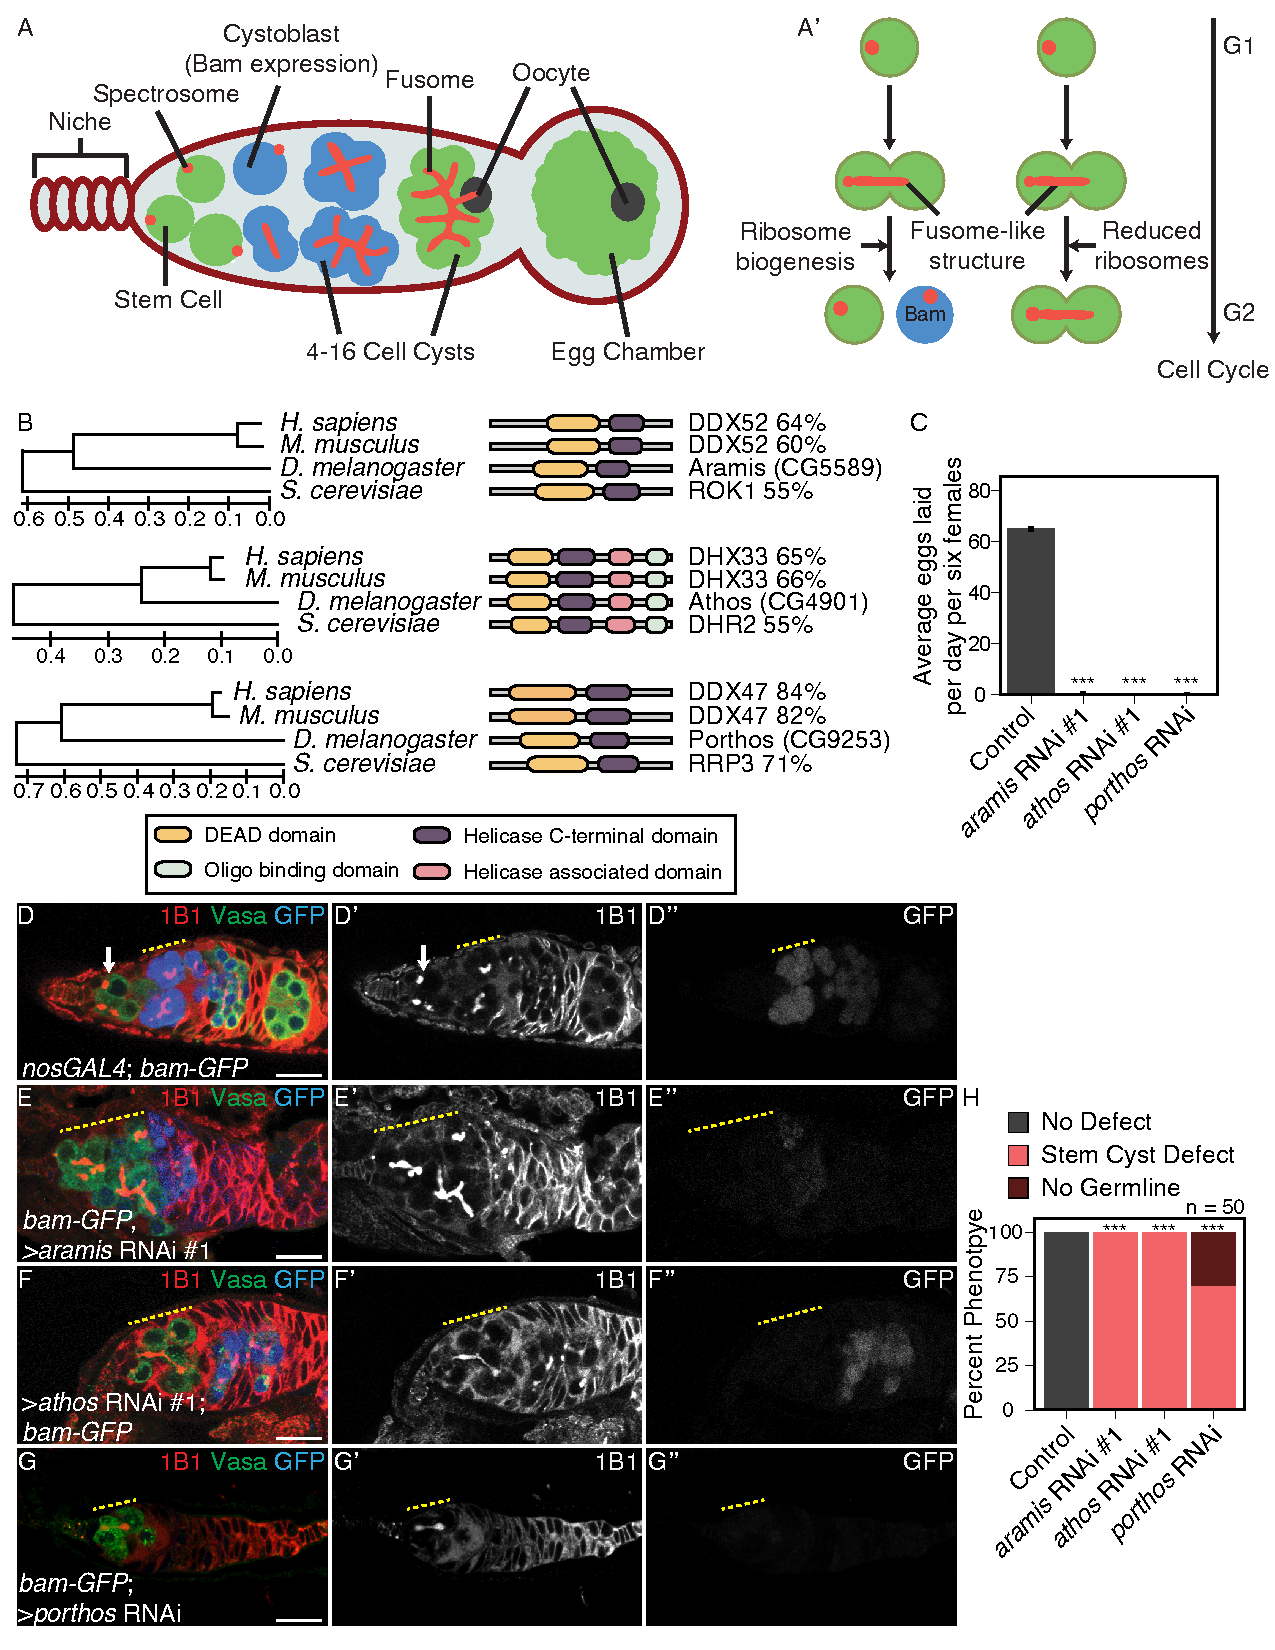
\includegraphics[width=6.5 in,height=8.9375 in]{./figure/Ribosome Biogenesis/Ribosome Biogenesis 1} 

}

\caption[\textbf{RNA helicases Aramis, Athos and Porthos are required for GSC differentiation.}]{\textbf{RNA helicases Aramis, Athos and Porthos are required for GSC differentiation.}}\label{fig:unnamed-chunk-6}
\end{figure}
\setstretch{1.0}

\setlength\parindent{0pt}(\textbf{A}) Schematic of \emph{Drosophila} germarium. Germline stem cells are attached to the somatic niche (dark red). The stem cells divide and give rise to a stem cell and a cystoblast (CB) that expresses the differentiation factor Bag-of-marbles (Bam). GSCs and CBs are marked by spectrosomes. The CB undergoes four incomplete mitotic divisions giving rise to a 16-cell cyst (blue). Cysts are marked by branched spectrosome structures known as fusomes (red). One cell of the 16-cell cyst is specified as the oocyte. The 16-cell cyst is encapsulated by the surrounding somatic cells giving rise to an egg chamber. (\textbf{A'}) Ribosome biogenesis promotes GSC cytokinesis and differentiation. Disruption of ribosome biogenesis results in undifferentiated stem cyst accumulation. (\textbf{B}) Conservation of \emph{aramis}, \emph{athos}, and \emph{porthos} between \emph{H. sapiens}, \emph{D. melanogaster}, and \emph{S. cerevisiae} (left), trees are drawn to scale, with branch lengths measured in the number of substitutions per site. Representation of conserved protein domains for three RNA helicases in \emph{Drosophila} compared to \emph{H. sapiens} and \emph{S. cerevisiae} orthologs (right). Percentage values represent similarity to \emph{Drosophila} orthologs. (\textbf{C}) Egg laying assay after germline RNAi knockdown of \emph{aramis}, \emph{athos} or \emph{porthos} indicating a loss of fertility compared to \emph{nosGAL4}, driver control (n=3 trials). *** = p \textless{} 0.001, Tukey's post-hoc test after one-way ANOVA, p \textless{} 0.001. Error bars represent standard error (SE). (\textbf{D-G''}) Confocal micrographs of ovaries from control, \emph{UAS-Dcr2; nosGAL4; bam-GFP} (\textbf{D-D''}) and germline RNAi depletion targeting (\textbf{E-E''}) \emph{aramis}, (\textbf{F-F''}) \emph{athos} or (\textbf{G-G''}) \emph{porthos} stained for 1B1 (red, left grayscale), Vasa (green), and Bam-GFP (blue, right grayscale). Depletion of these genes (\textbf{E-G''}) results in a characteristic phenotype in which early germ cells are connected marked by a 1B1 positive, fusome-like structure highlighted by a yellow dotted line in contrast to the single cells present in (\textbf{D-D''}) controls (white arrow) or differentiating cysts (yellow dashed line). Bam expression, if present, is followed by loss of the germline. (\textbf{H}) Phenotype quantification of ovaries depleted of \emph{aramis}, \emph{athos} or \emph{porthos} compared to control ovaries (n=50 ovarioles, df=2, *** = p \textless{} 0.001, Fisher's exact tests with Holm-Bonferroni correction). Scale bars are 15 micron.

\setstretch{2.0}

\textbf{\\
}

Aberrant cyst formation proximal to the niche could reflect stem cysts with GSCs that divide to give rise to CBs but fail to undergo cytokinesis or differentiated cysts that initiate differentiation but cannot progress further to form egg chambers. To discern between these possibilities, first we examined the expression of a marker of GSCs, phosphorylated Mothers against decapentaplegic (pMad). We observed pMad expression in the cells closest to the niche, but not elsewhere in the germline cysts of \emph{aramis}, \emph{athos}, and \emph{porthos} germline RNAi flies (\textbf{Figure 2.2H-H')} (Kai \& Spradling, 2003). Additionally, none of the cells connected to the GSCs in \emph{aramis}, \emph{athos}, and \emph{porthos} germline RNAi flies expressed the differentiation reporter \emph{bamGFP} (\textbf{Figure 2.1D-G'')} ({\textbf{???}}). Thus, loss of \emph{aramis}, \emph{athos}, or \emph{porthos} in the germline results in the formation of stem cysts, however with variable severity. This variability could be due to a differential requirement for these genes or different RNAi efficiencies. Overall, we infer that Aramis, Athos, and Porthos are required for proper GSC cytokinesis to produce a stem cell and differentiating daughter.
\begin{figure}

{\centering \includegraphics[width=6.5 in,height=8.9375 in]{./figure/Ribosome Biogenesis/Ribosome Biogenesis 1S} 

}

\caption[\textbf{Aramis, Athos, and Porthos are required for proper cytokinesis and differentiation, related to Figure 2.1.}]{\textbf{Aramis, Athos, and Porthos are required for proper cytokinesis and differentiation, related to Figure 2.1.}}\label{fig:unnamed-chunk-7}
\end{figure}
\setstretch{1.0}

\setlength\parindent{0pt}(\textbf{A}) qPCR targeting \emph{aramis}, \emph{athos}, \emph{porthos} relative to \(\alpha\)\emph{-tub84B} to measure knockdown efficiency of \emph{aramis}, \emph{athos}, and \emph{porthos} RNAi in the germline (n=3, Welch's t-test with Holm-Bonferroni correction, * =p\textless0.05, **=p\textless0.01). (\textbf{B-B'}) Confocal images of (\textbf{B}) Aramis::GFP::3XFLAG and (\textbf{B'}) Aramis::GFP::3XFLAG in conjunction with \emph{aramis} germline knockdown stained for Vasa (blue), and GFP (green). (\textbf{C-C'}) Confocal images of (\textbf{C}) Athos::GFP::3XFLAG and (\textbf{C'}) Athos::GFP::3XFLAG in conjunction with \emph{athos} germline knockdown stained for Vasa (blue), and GFP (green), early germline is outlined in yellow, representative somatic cell indicated by arrow. (\textbf{D}) Quantification of germline expression of GFP normalized to somatic GFP expression in Aramis::GFP::3XFLAG ovaries compared to Aramis::GFP::3XFLAG in conjunction with \emph{aramis} germline knockdown and Athos::GFP::3XFLAG ovaries compared to Athos::GFP::3XFLAG in conjunction with \emph{athos} germline knockdown showing that \emph{aramis} RNAi and \emph{athos} RNAi efficiently knockdown their targets in the germline. (n=14-15, Welch's t-test with Holm-Bonferroni correction, ***=p\textless0.001) (\textbf{E-E'''}) Confocal images of (\textbf{E}) \emph{nosGAL4}, driver control and germline RNAi knockdown using additional RNAi lines for (\textbf{E'}) \emph{aramis} and (\textbf{E''}) \emph{athos} stained for 1B1 (red) and Vasa (green). (\textbf{E'''}) Quantification of percentage of germaria with no defect (black), stem-cysts (salmon), or germline loss (dark red) in ovaries depleted of \emph{athos}, \emph{aramis}, or \emph{porthos} compared to control ovaries recapitulates the phenotypes with independent RNAi lines (n=50, df=2, *** = p\textless0.001, Fisher's exact test with Holm-Bonferroni correction). (\textbf{F-F'''}) Confocal images of germaria stained for 1B1 (red) and Phospho-tyrosine (green). Ring canals, marked by Phosopho-tyrosine, connect differentiating cysts in (\textbf{F}) control \emph{nosGAL4} ovaries and in between the interconnected cells of ovaries depleted of (\textbf{F'}) \emph{aramis}, (\textbf{F''}) \emph{athos}, or (\textbf{F'''}) \emph{porthos} with 1B1 positive structures going through the ring canals. (\textbf{G-G'''}) Confocal images of ovarioles stained for 1B1 (red) and Vasa (green). Control, \emph{nosGAL} ovaries have egg chambers while ovaries depleted of (\textbf{G'}) \emph{aramis}, (\textbf{G''}) \emph{athos}, or (\textbf{G'''}) \emph{porthos} lack egg chambers. (\textbf{H-H'''}) Confocal images of germaria stained for pMad (red, grayscale) and Vasa (green). In (\textbf{H}) control ovaries nuclear pMad staining occurs in cells proximal to the niche marking GSCs. Nuclear pMad staining in ovaries depleted of (\textbf{H'}) \emph{aramis}, (\textbf{H''}) \emph{athos}, and (\textbf{H'''}) \emph{porthos} demonstrates that the observed cysts are not composed of GSCs. Scale bar for main images is 15 micron, scale bar for insets is 3.75 micron.

\setstretch{2.0}

\textbf{\\
}

\hypertarget{athos-aramis-and-porthos-are-required-for-ribosome-biogenesis}{%
\subsection{Athos, Aramis, and Porthos are required for ribosome biogenesis}\label{athos-aramis-and-porthos-are-required-for-ribosome-biogenesis}}

We found that Aramis, Athos, and Porthos are conserved from yeast to humans (\textbf{Figure 2.1B}). The closest orthologs of Aramis, Athos, and Porthos are Rok1, Dhr2, and Rrp3 in yeast and DExD-Box Helicase 52 (DDX52), DEAH-Box Helicase 33 (DHX33), and DEAD-Box Helicase 47 (DDX47) in humans, respectively ({\textbf{???}}). Both the yeast and human orthologs have been implicated in rRNA biogenesis ({\textbf{???}}; {\textbf{???}}; {\textbf{???}}; {\textbf{???}}; {\textbf{???}}; {\textbf{???}}; {\textbf{???}}; {\textbf{???}}; {\textbf{???}}; {\textbf{???}}). In addition, the GSC-cytokinesis defect that we observed in \emph{aramis}, \emph{athos}, and \emph{porthos} RNAi flies is a hallmark of reduced ribosome biogenesis in the germline ({\textbf{???}}). Based on these observations, we hypothesized that Aramis, Athos, and Porthos could enhance ribosome biogenesis to promote proper GSC differentiation.

Many factors involved in rRNA biogenesis localize to the nucleolus and interact with rRNA ({\textbf{???}}; {\textbf{???}}; {\textbf{???}}; Arabi et al., 2005). To detect the subcellular localization of Aramis and Athos, we used available lines that express Aramis::GFP::FLAG or Athos::GFP::FLAG fusion proteins under endogenous control. For Porthos, we expressed a Porthos::FLAG::HA fusion under the control of UASt promoter in the germline using a previously described approach ({\textbf{???}}). We found that in the germline, Aramis, Athos and Porthos colocalized with Fibrillarin, which marks the nucleolus, the site of rRNA synthesis (\textbf{Figure 2.3A-C'''}) ({\textbf{???}}). Aramis was also in the cytoplasm of the germline and somatic cells of the gonad. To determine if Aramis, Athos, and Porthos directly interact with rRNA, we performed immunoprecipitation (IP) followed by RNA-seq. We found that rRNA immunopurified with Aramis, Athos, and Porthos \textbf{(Figure 2.3D-D'', Figure 2.4A-A'')}. Thus, Aramis, Athos, and Porthos are present in thenucleolus and interact with rRNA, suggesting that they might regulate rRNA biogenesis.
\begin{figure}

{\centering 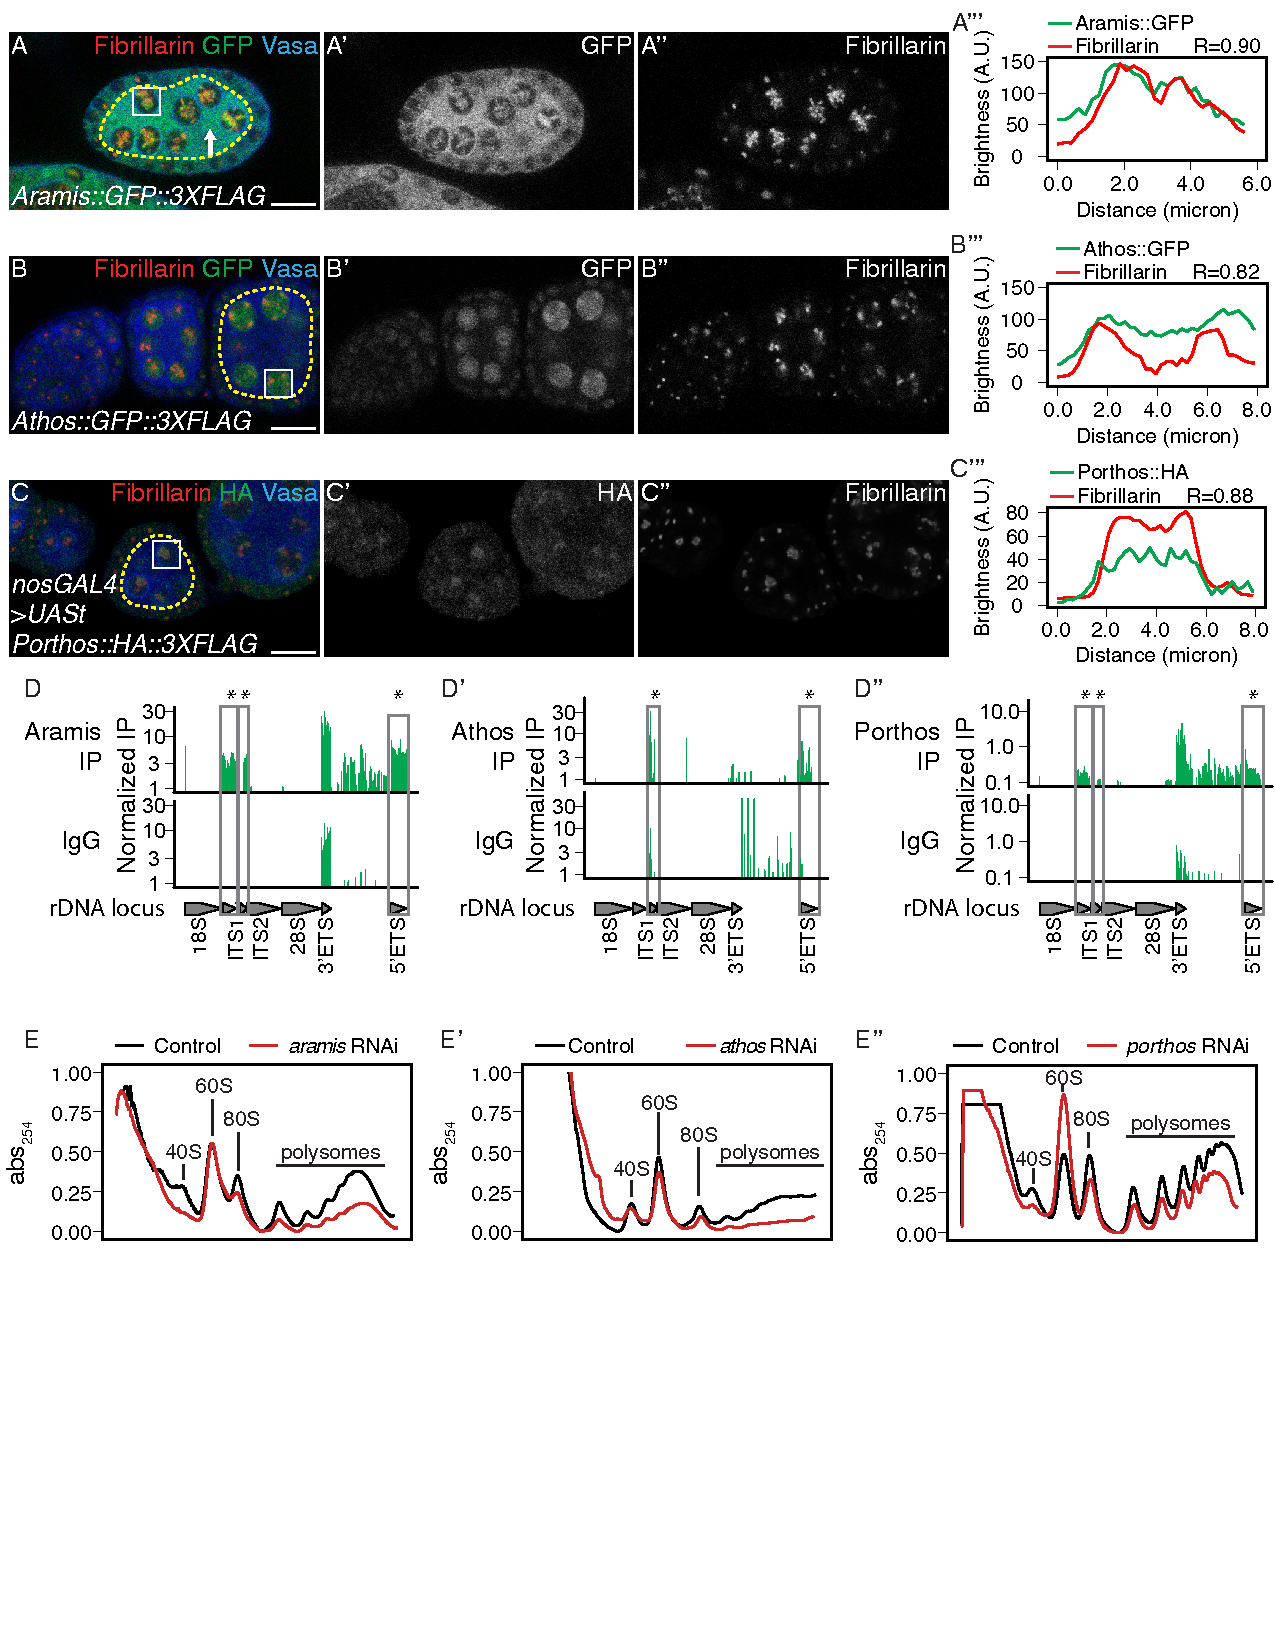
\includegraphics[width=6.5 in,height=6.347059 in]{./figure/Ribosome Biogenesis/Ribosome Biogenesis 2} 

}

\caption[\textbf{Athos, Aramis, and Porthos are required for efficient ribosome biogenesis.}]{\textbf{Athos, Aramis, and Porthos are required for efficient ribosome biogenesis.}}\label{fig:unnamed-chunk-8}
\end{figure}
\setstretch{1.0}

\setlength\parindent{0pt}(\textbf{A-C''}) Confocal images of ovariole immunostained for Fibrillarin (red, right grayscale), Vasa (blue), (\textbf{A-A''}) Aramis::GFP, (\textbf{B-B''}) Athos::GFP and (\textbf{C-C''}) Porthos::HA (green, left grayscale). (\textbf{A'''-C'''}) Fluorescence intensity plot generated from a box of averaged pixels centered around the punctate of Fibrillarin in the white box. The white box also indicates a nucleus, while the yellow dotted outline indicates the divide between soma and germline, with the germline on the interior of the outline and soma on the exterior. R values denote Spearman correlation coefficients between GFP and Fibrillarin from plot profiles generated using Fiji, taken from the nucleolus denoted by the white box. Aramis, Athos and Porthos are expressed throughout oogenesis and localize to the nucleolus. Aramis is also present in the cytoplasm. (\textbf{D-D''}) RNA IP-seq of (\textbf{D}) Aramis, (\textbf{D'}) Athos, and (\textbf{D''}) Porthos aligned to rDNA locus displayed as genome browser tracks. Bar height represents log scaled rRNA reads mapping to rDNA normalized to input and spike-in. Grey boxes outline ETS (external spacers) and ITS (internal spacers) which are only present in pre-rRNA that are significantly enriched in the IP compared to the IgG control (bootstrapped paired t-tests, n=3, * = p-value \textless{} 0.05). (\textbf{E-E''}) Polysome traces from \emph{Drosophila} S2 cells treated with dsRNA targeting \emph{aramis}, (\textbf{E'}) \emph{athos}, (\textbf{E'}) \emph{porthos} (red line) compared to a mock transfection control (black line). \emph{aramis}, athos and porthos are required to maintain a proper 40S/60S ribosomal subunit ratio compared to control and have a smaller 40S/60S ratio. \emph{athos} is required to maintain a proper 40S/60S ribosomal subunit ratio compared to control and has a larger 40S/60S ratio. Additionally, \emph{aramis}, \emph{athos}, and \emph{porthos} are required to maintain polysome levels. All three helicases are required to maintain polysome levels. Scale bar for all images is 15 micron.

\setstretch{2.0}

\textbf{\\
}

Nucleolar size, and in particular nucleolar hypotrophy, is associated with reduced ribosome biogenesis and nucleolar stress ({\textbf{???}}; {\textbf{???}}). If Aramis, Athos, and Porthos promote ribosome biogenesis, then their loss would be expected to cause nucleolar stress and a reduction in mature ribosomes. Indeed, immunostaining for Fibrillarin revealed hypotrophy of the nucleolus in \emph{aramis, athos,} and \emph{porthos} germline RNAi flies compared to in control flies, consistent with nucleolar stress (\textbf{Figure 2.3B-C'}). Next, we used polysome profile analysis to evaluate the ribosomal subunit ratio and translation status of ribosomes in S2 cells depleted of \emph{aramis}, \emph{athos}, or \emph{porthos} ({\textbf{???}}; {\textbf{???}}). We found that upon the depletion of all three helicases, the heights of the polysome peaks were reduced (\textbf{Figure 2.3E-E''}). We found that depletion of \emph{aramis} and \emph{porthos} diminished the height of the 40S subunit peak compared to the 60S subunit peak, characteristic of defective 40S ribosomal subunit biogenesis (\textbf{Figure 2.3E, E''}, \textbf{Figure 2.4D)} (Cheng et al., 2019), whereas \emph{athos} depletion diminished the height of the 60S subunit peak compared to the 40S peaks, characteristic of a 60S ribosomal subunit biogenesis defect (\textbf{Figure 2.3E', Figure 2.4D'}) (Cheng et al., 2019). Previous work indicates that the stem-cyst that arises from depletion of genes involved in ribosome biogenesis in the germline genetically interacts with Shrub (shrb) a member of the Escrt-III complex. To further determine if \emph{aramis}, \emph{athos}, and \emph{porthos} regulates ribosome biogenesis, we performed trans-heterozygous crosses between \emph{aramis}, \emph{athos}, and \emph{porthos} and \emph{shrb}. We observed the presence of stem-cyst structures even heterozygotes mutants of \emph{shrb}, consistent with previous observations ({\textbf{???}}; {\textbf{???}}), and in \emph{aramis}, or \emph{athos}, \emph{porthos}. We found that in trans-heterozygous germaria of a \emph{shrb} mutant our genes of interest result in a more frequent occurrence of stem-cysts than in their respective heterozygous background consistent with their role in ribosome biogenesis (\textbf{Figure S2.4E-L}). Taken together our findings indicate that these helicases promote ribosome biogenesis in \emph{Drosophila}.
\begin{figure}

{\centering 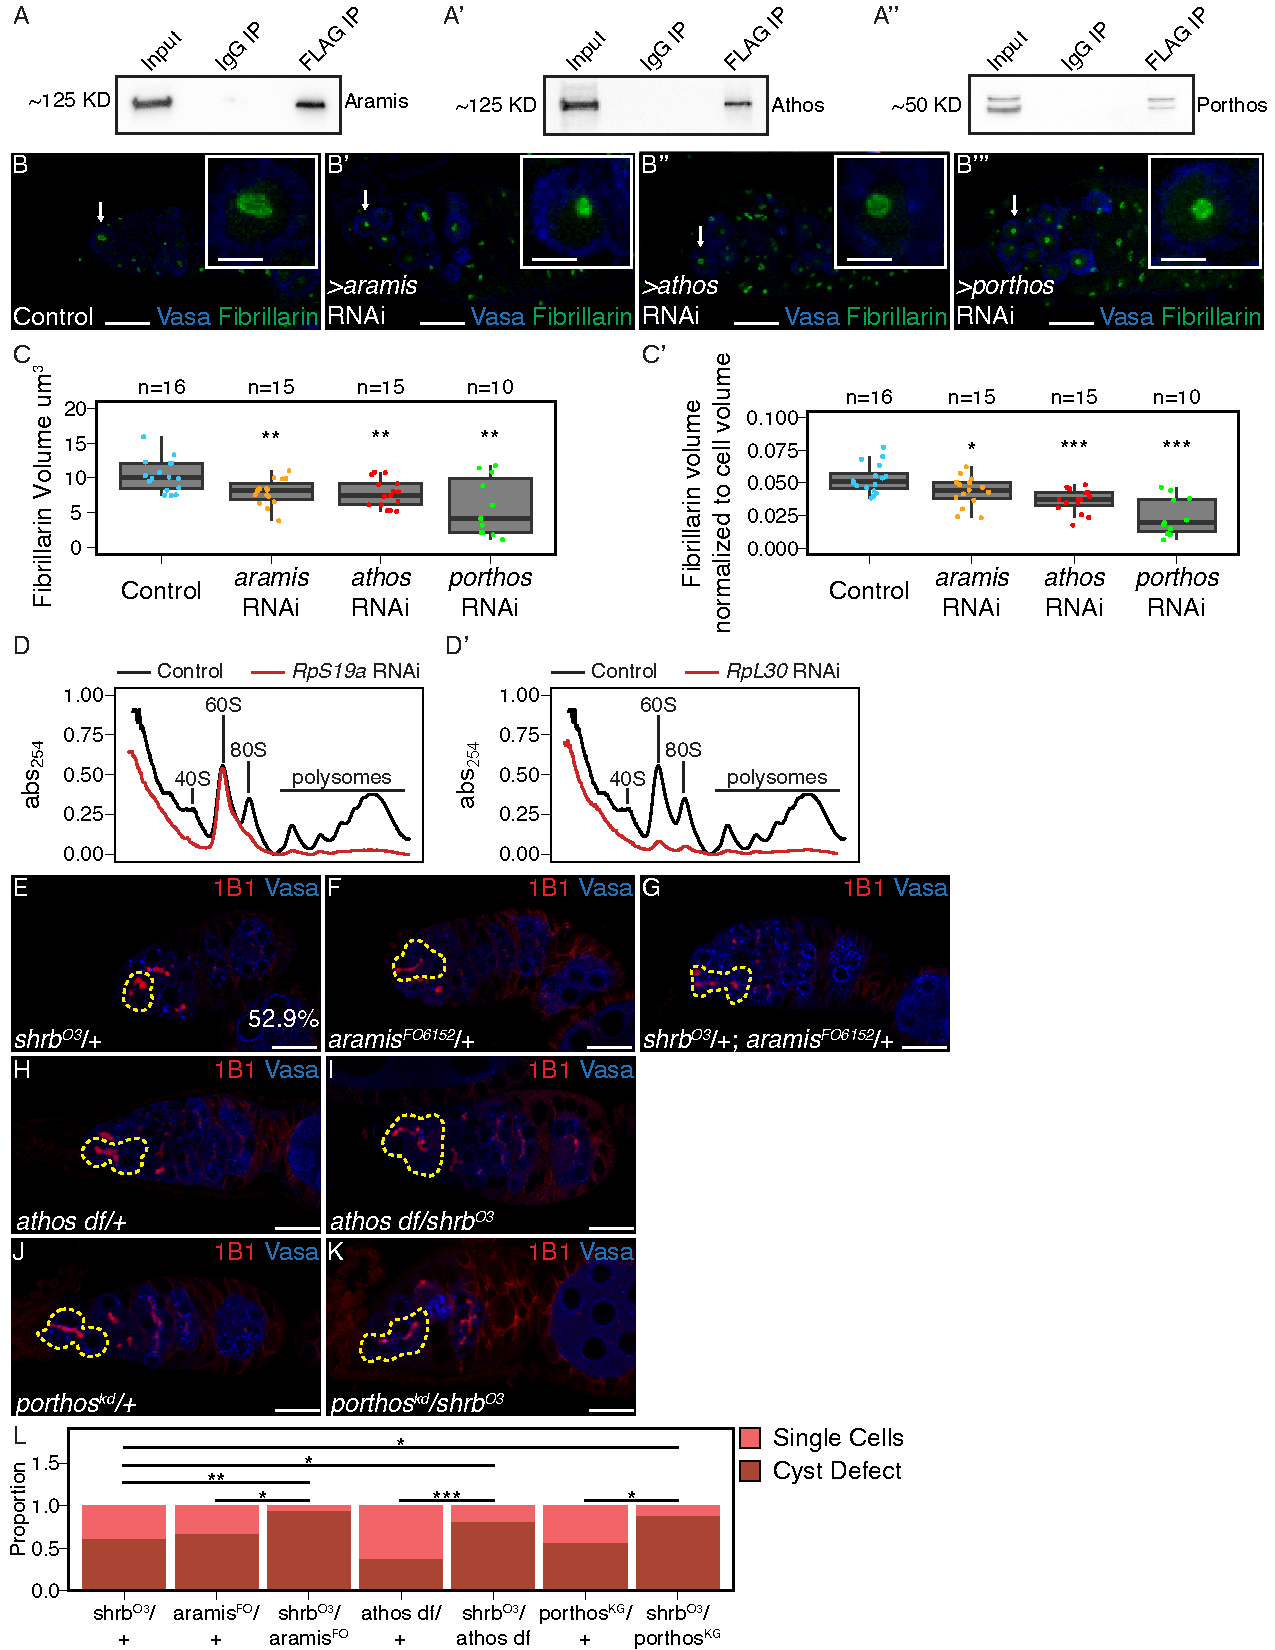
\includegraphics[width=6.5 in,height=8.9375 in]{./figure/Ribosome Biogenesis/Ribosome Biogenesis 2S} 

}

\caption[\textbf{Athos, Aramis, and Porthos are required for efficient ribosome biogenesis., related to Figure 2.3.}]{\textbf{Athos, Aramis, and Porthos are required for efficient ribosome biogenesis., related to Figure 2.3.}}\label{fig:unnamed-chunk-9}
\end{figure}
\setstretch{1.0}

\setlength\parindent{0pt}(\textbf{A-A''}) Western blots of immunoprecipitations from ovaries for FLAG-tagged (\textbf{A}) Aramis, (\textbf{A'}) Athos, and (\textbf{A''}) Porthos. (\textbf{B-B'''}) Confocal images of (\textbf{B}) \emph{nosGAL4}, driver control, (\textbf{B'}) \emph{aramis} (\textbf{B''}) \emph{athos} and (\textbf{B'''}) \emph{porthos} germline RNAi germaria stained for Fibrillarin (green), and Vasa (blue). (\textbf{C-C'}) Quantification of (\textbf{C}) raw nucleolar volume or (\textbf{C'}) normalized to cell volume nucleolar volume in GSCs of \emph{aramis}, \emph{athos}, and \emph{porthos} RNAi, compared to control indicates loss of each helicase results in nucleolar stress. (n=12-16 GSCs per genotype, One-way ANOVA, p\textless0.001, with Welch's t-test, Holm-Bonferroni corrected, * = p\textless0.05, ** = p\textless0.01, *** = p\textless0.001). (\textbf{D-D'}) Polysome preparations from \emph{Drosophila} S2 cells in cells treated with dsRNA targeting (\textbf{D}) \emph{RpS19a} or (\textbf{D'}) \emph{RpL30} (red line) compared to a mock transfection control (black line). (\textbf{E-K}) Confocal images of heterozygous (\textbf{E}) \emph{shrb}\textsuperscript{O3}/+, (\textbf{F}) \emph{aramis}\textsuperscript{f06152}/+ mutant ovaries, (\textbf{G}) \emph{shrb}\textsuperscript{O3}/+; \emph{aramis}\textsuperscript{f06152}/+ transheterozygous, (\textbf{H}) \emph{athos} deficiency/+ mutant ovaries, (\textbf{I}) \emph{athos} deficiency/\emph{shrb}\textsuperscript{O3} transheterozygous, heterozygous (\textbf{J}) \emph{porthos}\textsuperscript{KG05120}/+ mutant ovaries and (\textbf{K}) \emph{porthos}\textsuperscript{KG05120}/\emph{shrb}\textsuperscript{O3} transheterozygous ovaries stained for 1B1 (red) and Vasa (blue). (\textbf{L}) Quantification of proportion of germaria with presence of a stem-cyst or single cells from the indicated genotypes (pairwise one-sided Fisher's tests, Holm-Bonferroni corrected, * = p\textless0.05, ** = p\textless0.01, *** = p\textless0.001). Scale bar for main images is 15 micron, scale bar for insets is 3.75 micron.

\setstretch{2.0}

\textbf{\\
}

\hypertarget{aramis-promotes-cell-cycle-progression-via-p53-repression}{%
\subsection{Aramis promotes cell cycle progression via p53 repression}\label{aramis-promotes-cell-cycle-progression-via-p53-repression}}

Our data so far indicate that Aramis, Athos and Porthos promote ribosome biogenesis, which is known to be required for GSC abscission ({\textbf{???}}). Yet the connections between ribosome biogenesis and GSC abscission are poorly understood. To explore the connection, we further examined the \emph{aramis} germline RNAi line, as its defect was highly penetrant but maintained sufficient germline for analysis (\textbf{Figure 2.1E, H}). First, we compared the mRNA profiles of \emph{aramis} germline RNAi ovaries to \emph{bam} germline RNAi to determine if genes that are known to be involved in GSC abscission have altered expression. We used germline \emph{bam} depletion as a control because it leads to the accumulation of CBs with no abscission defects ({\textbf{???}}; {\textbf{???}}; {\textbf{???}}; Ohlstein \& McKearin, 1997), whereas loss of \emph{aramis} resulted in accumulation of CBs that do not abscise from the GSCs.

We performed RNA-seq and found that 607 RNAs were downregulated and 673 RNAs were upregulated in \emph{aramis} germline RNAi versus \emph{bam} germline RNAi (cut-offs for differential gene expression were log\textsubscript{2}(foldchange) \textgreater\textbar1.5\textbar, FDR \textless{} 0.05) (\textbf{Figure 2.10A, Supplemental Table 2.2}). Gene Ontology (GO) analysis for biological processes on these genes encoding these differentially expressed mRNAs ({\textbf{???}}) revealed that the genes that were downregulated upon \emph{aramis} germline depletion were enriched for GO terms related to the cell cycle, whereas the upregulated genes were enriched for GO terms related to stress response (\textbf{Figure 2.5A, Figure 2.6B}). The downregulated genes included \emph{Cyclin A}, which is required for cell cycle progression, \emph{Cyclin B} (\emph{CycB}) and \emph{aurora B}, which are required for both cell cycle progression and cytokinesis; in contrast the housekeeping gene \emph{Actin 5C} was unaffected (\textbf{Figure 2.5B-C, Figure 2.6C-C'}) ({\textbf{???}}; {\textbf{???}}). We confirmed that CycB was reduced in the ovaries of \emph{aramis} germline RNAi flies compared to \emph{bam} germline RNAi flies by immunofluorescence (\textbf{Figure 2.5D-F}). These changes to genes that promote cell cycle and cytokinesis were also seen \emph{aramis; bam} double depletions as the Biological Process GO-terms we identified from targets downregulated in \emph{aramis} RNAi were very similar to those we identified from in \emph{bam} RNAi; \emph{aramis} RNAi compared to their controls (\textbf{Figure 2.5A, Supplemental Table 2.3}). Similarly, all of the GO-terms we identified in from upregulated genes are also enriched GO terms from the double-knockdown upregulated targets (\textbf{Figure 2.6B, Supplemental Table 2.3}). Crucially, all the genes we refer to in the manuscript such as \emph{CycB}, \emph{AurB,} and \emph{CycA} are also targets in \emph{bam} RNAi; \emph{aramis} RNAi. (\textbf{Figure 2.6B, Supplemental Table 2.3}). These results suggest that \emph{aramis} is required for the proper expression of key regulators of GSC abscission.

CycB is expressed during G2 phase after asymmetric cell division to promote GSC abscission ({\textbf{???}}; {\textbf{???}}). To test if the loss of germline \emph{aramis} leads to GSC abscission defects due to diminished expression of CycB, we attempted to express a functional CycB::GFP fusion protein in the germline under the control of a UAS/GAL4 system (\textbf{Figure 2.6F-G'}) ({\textbf{???}}). Unexpectedly, the CycB::GFP fusion protein was not expressed in the \emph{aramis-}depleted germline, unlike the wild type (WT) germline (\textbf{Figure 2.6F-G}) ({\textbf{???}}; {\textbf{???}}; {\textbf{???}}). We considered the possibility that progression into G2 is blocked in the absence of \emph{aramis}, precluding expression of CycB. To monitor the cell cycle, we used the Fluorescence Ubiquitin-based Cell Cycle Indicator (FUCCI) system. \emph{Drosophila} FUCCI utilizes a GFP-tagged degron from E2f1 to mark G2, M, and G1 phases and an RFP-tagged degron from CycB to mark S, G2, and M phases ({\textbf{???}}). We observed cells in different cell cycle stages in both WT and \emph{bam}-depleted germaria, but the \emph{aramis}-depleted germaria expressed neither GFP nor RFP (\textbf{Figure 2.6F-H''}). Double negative reporter expression is thought to indicate early S phase, when expression of E2f1 is low and CycB is not expressed ({\textbf{???}}). The inability to express FPs is not due to a defect in translation as \emph{aramis}-depleted germline can express GFP that is not tagged with the degron (\textbf{Figure 2.6K}). Taken together, we infer that loss of \emph{aramis} blocks cell cycle progression around late G1 phase/early S phase and prevents progression to G2 phase, when GSCs abscise from CBs.
\begin{figure}

{\centering \includegraphics[width=6.5 in,height=8.9375 in]{./figure/Ribosome Biogenesis/Ribosome Biogenesis 3} 

}

\caption[\textbf{Athos, Aramis, and Porthos are required for cell cycle progression during early oogenesis.}]{\textbf{Athos, Aramis, and Porthos are required for cell cycle progression during early oogenesis.}}\label{fig:unnamed-chunk-10}
\end{figure}
\setstretch{1.0}

\setlength\parindent{0pt}(\textbf{A}) Bar plot representing the most significant Biological Process GO-terms of downregulated genes in ovaries depleted of \emph{aramis} compared to \emph{bam} RNAi control (FDR = False Discovery Rate from p-values using a Fisher's exact test). (\textbf{B-C}) Genome browser tracks representing the gene locus of (\textbf{B}) \emph{CycB} and (\textbf{C}) \emph{aurora B} in ovaries depleted of \emph{aramis} compared to the developmental control, \emph{bam} RNAi. Y-axis represents the number of reads mapping to the locus in bases per million (BPM). (\textbf{D-E''}) Confocal images of germaria stained for CycB (red, left grayscale) and Vasa (blue, right grayscale) in (\textbf{D-D'''}) \emph{bam} RNAi control ovaries and (\textbf{E-E''}) \emph{aramis} germline RNAi. (\textbf{F}) Boxplot of CycB intensity in the germline normalized to Cyc B intensity in the soma in \emph{bam} RNAi and \emph{aramis} RNAi (n=12-14 germaria per sample, *** = p\textless{} 0.001, Welch t-test. (\textbf{G-H''}) Confocal images of germaria stained for p53 (red, left grayscale), GFP (green), and Vasa (blue, right grayscale) in (\textbf{G-G''}) \emph{nosGAL4}, driver control ovaries and (\textbf{H-H''}) germline depletion of \emph{aramis}. Cells highlighted by a dashed yellow circle represent cell shown in the inset. Driver control \emph{nosGAL4} ovaries exhibit attenuated p53 expression in GSCs and CBs, but higher expression in cyst stages as previously reported, while p53 punctate are visible in the germline of \emph{aramis} RNAi in the undifferentiated cells. (\textbf{I}) Box plot of percentage of pixel area exceeding the background threshold for p53 in GSCs and CBs in driver control \emph{nosGAL4} ovaries and the germline of \emph{aramis} RNAi indicates p53 expression is elevated in the germline over the GSCs/CBs of control ovaries. (n=10 germaria per sample, *** = p \textless{} 0.001, Welch's t-test. (\textbf{J-K''}) Confocal images of germaria stained for 1B1 (red, left grayscale) and Vasa (blue, right grayscale) in (\textbf{J-J''}) germline \emph{aramis} RNAi in a wildtype background and (\textbf{K-K''}) germline \emph{aramis} RNAi with a mutant, null, \emph{p53\textsuperscript{5-A-14}} background showing presence of spectrosomes upon loss of p53. (\textbf{L}) Quantification of stem-cyst phenotypes demonstrates a significant rescue upon of loss of \emph{p53\textsuperscript{5-A-14}} in \emph{aramis} germline depletion compared to the control (n=43-55 germaria per genotype, df=2, Fisher's exact test p\textless{} 0.05). (\textbf{M-N}) Confocal images of ovaries stained for 1B1 (red) and Vasa (blue) in \emph{nosGAL4} ovaries (\textbf{M}) and ovaries overexpressing \emph{p53} in the germline. Cysts are denoted by a dotted yellow line, single cells by a white arrow. (\textbf{N}). We observed that 84\% of germaria from \emph{p53} overexpression ovaries had loss of germline while 12\% of germaria contained a cyst, marked by an extended spectrosome structure connecting germline cells together, and an additional 4\% of germaria contained an accumulation of single cells (n=55 germaria, Fisher's exact test, p\textless0.001). Scale bar for main images is 15 micron, scale bar for insets is 3.75 micron

\setstretch{2.0}

\textbf{\\
}

In mammals, cells defective for ribosome biogenesis stabilize p53, which is known to impede the G1 to S transition ({\textbf{???}}; {\textbf{???}}). Therefore, we hypothesized that the reduced ribosome biogenesis in the \emph{aramis}-depleted germline leads to p53 stabilization in undifferentiated cells, driving cell cycle arrest and GSC abscission defects. To test this hypothesis, we detected p53 and Vasa in the germline by immunostaining. A hybrid dysgenic cross that expresses p53 in undifferentiated cells was utilized as a positive control, and \emph{p53} null flies were used as negative controls (\textbf{Figure 2.6L-M}) ({\textbf{???}}). In WT, we observed p53 expression in the meiotic stages of germline but p53 expression in GSCs and CBs was attenuated as previously reported (\textbf{Figure 2.5G-G''}) (Lu, Chapo, Roig, \& Abrams, 2010). However, compared to WT GSCs/CBs, we observed p53 expression in the stem cysts of the \emph{aramis-}depleted germline (\textbf{Figure 2.5G-I}). Similarly, we observed p53 expression in the stem cysts of \emph{athos-} and \emph{porthos-}depleted germlines (\textbf{Figure 2.6N-O}), further supporting that reduced ribosome biogenesis stabilizes p53. To determine if p53 stabilization is required for the cell cycle arrest in \emph{aramis}, \emph{athos}, and \emph{porthos-}depleted germline cysts, we depleted \emph{aramis}, \emph{athos} and \emph{porthos} in the germline of \emph{p53} mutants using germline specific knockdown. We observed a partial but significant alleviation of the cyst phenotype, such that spectrosomes were restored (\textbf{Figure 2.5J-L, Figure 2.6P-T}). This finding indicates that p53 contributes to cytokinesis failure upon loss of \emph{aramis}, but that additional factors are also involved.

To determine if p53 stabilization is required for the cell cycle arrest in \emph{aramis-}, \emph{athos-}, and \emph{porthos-}depleted germline cysts, we depleted \emph{aramis}, \emph{athos} and \emph{porthos} in the germline of \emph{p53} mutants using germline specific knockdowns. We observed a partial but significant alleviation of the cyst phenotype, such that spectrosomes were restored (\emph{Figure 2.5M-N}), This finding indicates that p53 contributes to cytokinesis failure upon loss of \emph{aramis, athos} and \emph{porthos} but that additional factors are also involved. To determine if aberrant expression of p53 is sufficient to cause the formation of stem-cysts, we overexpressed p53 in the germline under the control of a UAS/GAL4 system. While 84\% of germaria had a complete loss of germline as previously reported ({\textbf{???}}), excitingly in 12\% of germaria the germline cells were connected by a fusome-like structure, phenocopying loss of \emph{aramis}, \emph{athos}, or \emph{porthos} (\textbf{Figure 3M-N}), and in the rest, we observed several single germline cells, compared to the control (n=55, Fisher's exact test, p\textless0.001). Taken together, we find that \emph{aramis-, athos-, and porthos-} depleted germ cells display reduced ribosome biogenesis, aberrant expression of p53 protein, and a block in cell cycle progression. Reducing p53 partially alleviates the cell cycle block and GSC cytokinesis defect, while inappropriate p53 expression results in loss of germline and cytokinesis defects in the GSCs., while inappropriate p53 expression results in loss of germline and cytokinesis defects.
\begin{figure}

{\centering \includegraphics[width=7 in,height=5.409091 in]{./figure/Ribosome Biogenesis/Ribosome Biogenesis 3S} 

}

\caption[\textbf{Aramis is required for proper cell cycle progression, related to Figure 2.5.}]{\textbf{Aramis is required for proper cell cycle progression, related to Figure 2.5.}}\label{fig:unnamed-chunk-11}
\end{figure}
\setstretch{1.0}

\setlength\parindent{0pt}(\textbf{A}) Biplot of mRNA levels in \emph{aramis} RNAi compared to \emph{bam} RNAi. Blue points represent mRNAs significantly upregulated \emph{aramis} RNAi compared to \emph{bam} RNAi, red points represent mRNAs significantly downregulated \emph{aramis} RNAi compared to \emph{bam} RNAi. (\textbf{B}) Bar plot representing the most significant Biological Process GO-terms of upregulated genes in ovaries depleted of \emph{aramis} compared to the developmental control, \emph{bam} RNAi. (\textbf{C-C'}) Genome browser tracks of mRNA levels at the (\textbf{C}) \emph{Cyclin} \emph{A} and (\textbf{C'}) \emph{Actin 5C} loci indicate that the RNAseq target gene \emph{Cyclin A} expression is downregulated, while a non-target, \emph{Actin 5C} is not downregulated. (\textbf{D-E'}) Confocal images of germaria stained for 1B1 (red, greyscale) and Vasa (blue) (\textbf{D-D'}) from ovaries with germline depletion of \emph{bam} and (\textbf{E-E'}) germline depletion of \emph{bam} and \emph{aramis} simultaneously demonstrates that simultaneous depletion of \emph{bam} and \emph{aramis} results in a stem-cyst similar to depletion of \emph{aramis} alone. (\textbf{F-G}) Confocal images of germaria stained for 1B1 (red), Vasa (blue), and Cyclin B::GFP (green) in (\textbf{F}) control and (\textbf{G}) germline depletion of \emph{aramis} demonstrates that functional Cyclin B::GFP cannot be efficiently expressed in germline depleted of \emph{aramis}. (\textbf{H-J''}) Confocal images of germaria that express Fly-FUCCI in the germline stained for Vasa (blue). GFP-E2f1\textsuperscript{degron} (green, right grayscale) and RFP-CycB\textsuperscript{degron} (red, left grayscale) in (\textbf{H-H''}) \emph{nosGAL4}, driver control ovaries, (\textbf{I-I''}) \emph{bam} RNAi as a developmental control, and (\textbf{J-J''}) ovaries with germline depletion \emph{of} \emph{aramis} demonstrates that the germline of \emph{aramis} RNAi germline depleted ovaries are negative for both G1 and G2 cell cycle markers. (\textbf{K}) Confocal images of \emph{aramis} germline RNAi expressing GFP in the germline, stained for 1B1 (red), Vasa (blue), and GFP (green) indicates productive translation of transgenes still occurs. (\textbf{L-M}) Confocal images of germaria stained for p53 (red) and Vasa (blue) in (\textbf{L}) hybrid dysgenic, Harwich, ovaries and (\textbf{M}) p53\textsuperscript{11-B-1} ovaries stained for p53 (red) and Vasa (blue) demonstrate the expected p53 staining patterns. (\textbf{N-O}) Confocal images of germaria stained for p53 (red) and Vasa (blue) in ovaries depleted of (\textbf{N}) \emph{athos} or (\textbf{O}) \emph{porthos} in the germline exhibit p53 punctate staining. Cells highlighted by a dashed yellow circle represent cells shown in the inset. (\textbf{P-Q}) Confocal images of germaria stained for 1B1 (red) and Vasa (blue) in (\textbf{P}) germline \emph{athos} RNAi in a wildtype background and (\textbf{Q}) germline \emph{athos} RNAi with a mutant, null, \emph{p53\textsuperscript{5-A-14}} background showing presence of spectrosomes upon loss of p53. (\textbf{R-S}) Confocal images of germaria stained for 1B1 (red) and Vasa (blue) in (\textbf{R}) germline \emph{porthos} RNAi in a wildtype background and (\textbf{S}) germline \emph{porthos} RNAi with a mutant, heterozygous, \emph{p53\textsuperscript{5-A-14}}/+ background showing presence of spectrosomes upon reduction of p53 (\textbf{T}) Phenotypic quantification of demonstrates a significant rescue upon of loss of \emph{p53\textsuperscript{5-A-14}} in germline \emph{athos} (n=63 \emph{athos}, n=47 \emph{athos} RNAi, \emph{p53\textsuperscript{5-A-14}}, Fisher's exact test p \textgreater{} 0.001) or \emph{porthos}-depletion (n=34 \emph{porthos} RNAi; n=41 \emph{porthos} RNAi, \emph{p53\textsuperscript{5-A-14}}/+, Fisher's exact test p \textgreater{} 0.001) compared to the respective control.

\setstretch{2.0}

\textbf{\\
}

\textbf{Aramis promotes translation of Non1, a negative regulator of p53, linking ribosome biogenesis to the cell cycle}

Although p53 protein levels were elevated upon loss of \emph{aramis} in the germline, \emph{p53} mRNA levels were not significantly altered (log\textsubscript{2} fold change: -0.49; FDR: 0.49). Given that ribosome biogenesis is affected, we considered that translation of p53 or one of its regulators was altered in \emph{aramis}-depleted germlines. To test this hypothesis, we performed polysome-seq of gonads enriched for GSCs or CBs as developmental controls, as well as gonads depleted for \emph{aramis} in the germline ({\textbf{???}}). We plotted the ratios of polysome-associated RNAs to total RNAs (\textbf{Figure 2.7A-A'', Supplemental Table 2.4}) and identified 87 mRNAs with a reduced ratio upon depletion of \emph{aramis}, suggesting that they were translated less efficiently compared to developmental controls. Loss of \emph{aramis} reduced the levels of these 87 downregulated transcripts in polysomes, without significantly affecting their total mRNA levels (\textbf{Figure 2.7B, Figure 2.8A-A'}). These 87 transcripts encode proteins mostly associated with translation including ribosomal proteins (\textbf{Figure 2.7C)}. To validate that Aramis regulates translation of these target mRNAs, we utilized a reporter line for the Aramis-regulated transcript encoding Ribosomal protein S2 (RpS2) that is expressed in the context of the endogenous promoter and regulatory sequences ({\textbf{???}}; {\textbf{???}}). We observed reduced levels of RpS2::GFP in germlines depleted of \emph{aramis} but not in those depleted of \emph{bam} (\textbf{Figure 2.7D-F}). RpS2::GFP expression is also reduced in \emph{bam} RNAi, \emph{aramis} RNAi double germline knockdown compared to \emph{bam} RNAi (\textbf{Figure 2.8B-D}). To ensure that reduced RpS2::GFP levels did not reflect a global decrease in translation, we visualized nascent translation using O-propargyl-puromycin (OPP). OPP is incorporated into nascent polypeptides and can be detected using click-chemistry ({\textbf{???}}). We observed that global translation in the germlines of ovaries depleted of \emph{aramis} was not reduced compared to single cells of control ovaries or \emph{bam} \textbf{(Figure 2.7G-J)}. Notably, the regulation of these genes do not appear to be directly mediated by Aramis as none of the target genes are enriched from Aramis::GFP::3XFLAG RNA IP-seq (\textbf{Supplemental Table 2.5}). Thus, loss of \emph{aramis} results in reduced translation of a subset of transcripts compared to the rest of the transcriptome.
\begin{figure}

{\centering 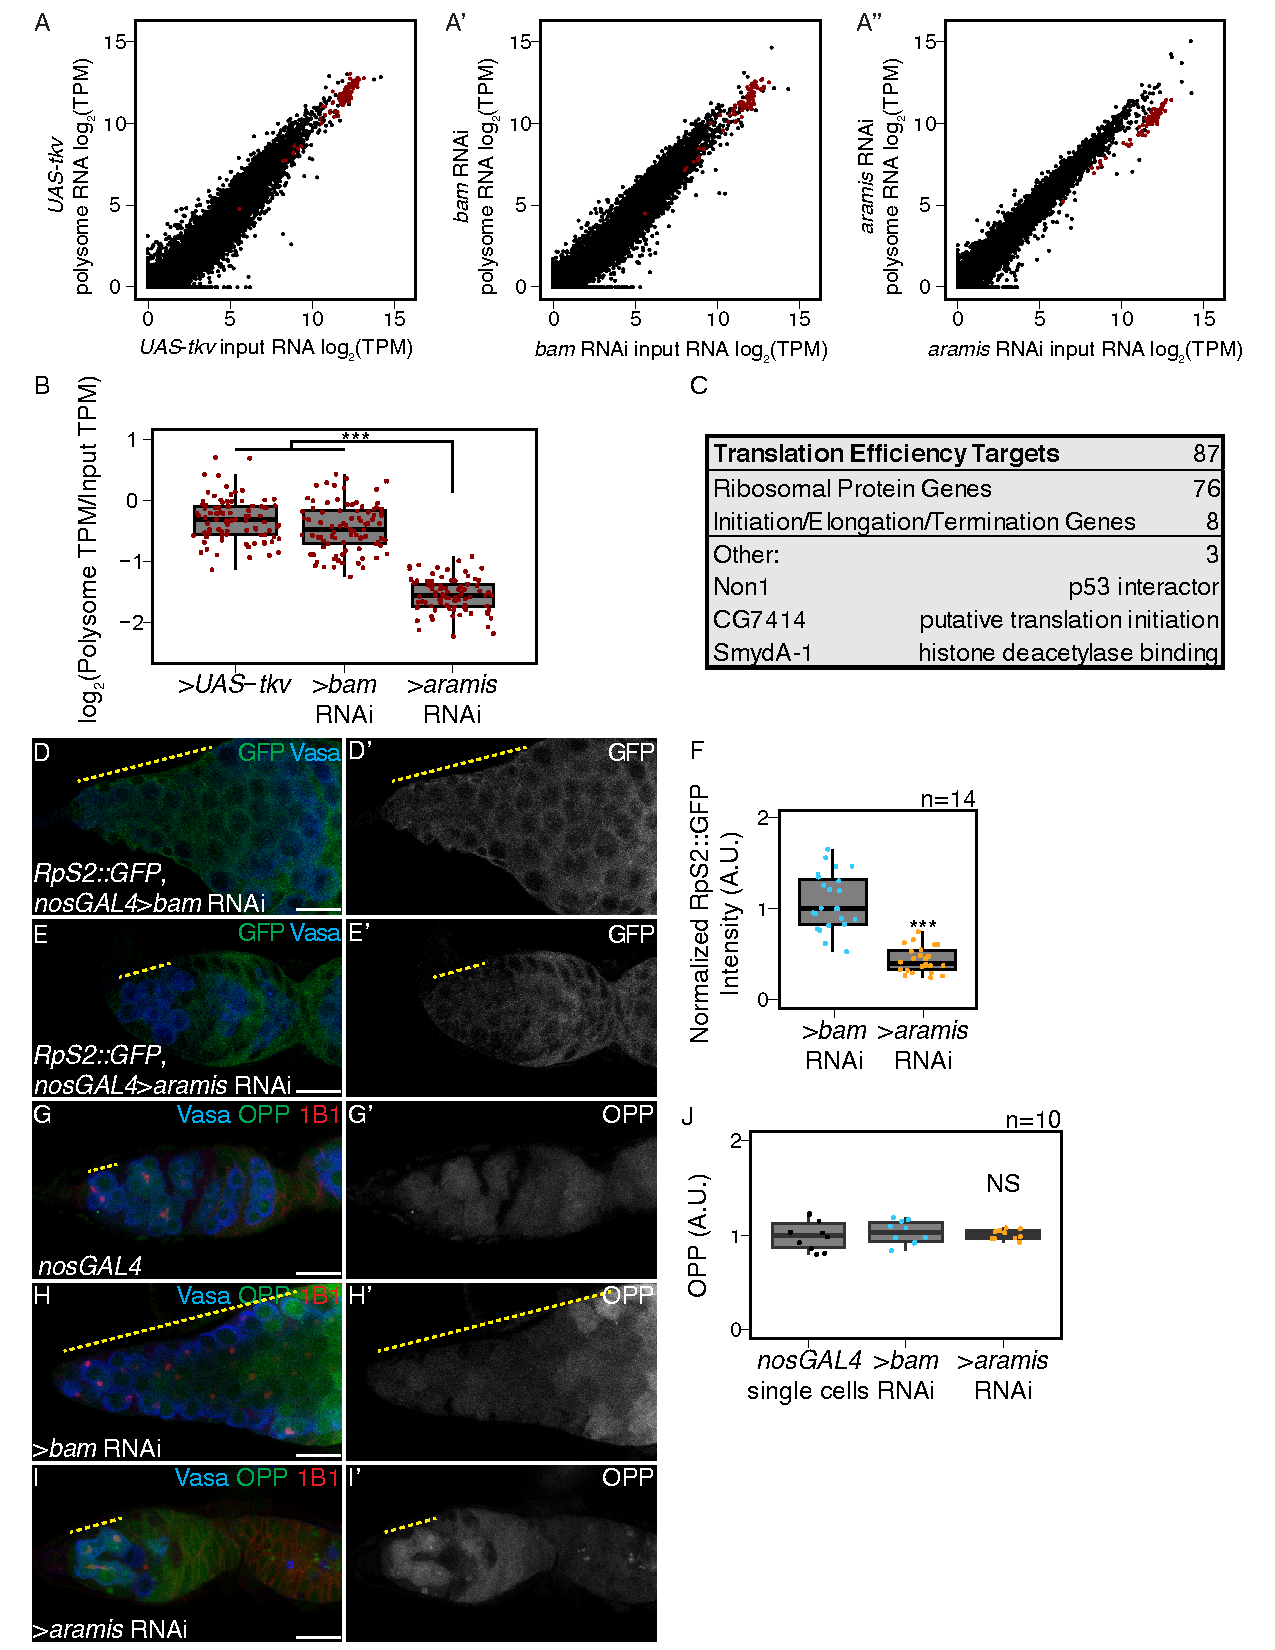
\includegraphics[width=6.5 in,height=8.9375 in]{./figure/Ribosome Biogenesis/Ribosome Biogenesis 4} 

}

\caption[\textbf{Aramis is required for efficient translation of a subset of mRNAs.}]{\textbf{Aramis is required for efficient translation of a subset of mRNAs.}}\label{fig:unnamed-chunk-12}
\end{figure}
\setstretch{1.0}

\setlength\parindent{0pt}(\textbf{A-A''}) Biplots of poly(A)+ mRNA Input versus polysome associated mRNA from (\textbf{A}) ovaries genetically enriched for GSCs (\emph{UAS-tkv}), (\textbf{A'}) Undifferentiated GSC daughter cells (\emph{bam} RNAi) or (\textbf{A''}) germline \emph{aramis} RNAi ovaries. (\textbf{B}) Boxplot of translation efficiency of target genes in \emph{UAS}-\emph{tkv}, \emph{bam} RNAi, and \emph{aramis} RNAi samples (ANOVA p\textless0.001, post-hoc Welch's t-test, n=87, *** = p \textless{} 0.001). (\textbf{C}) Summary of downregulated target genes identified from polysome-seq. (\textbf{D-E'}) Confocal images of germaria stained for 1B1 (red), RpS2::GFP (green, grayscale), and Vasa (blue) in (\textbf{D-D'}) \emph{bam} RNAi control and (\textbf{E-E'}) \emph{aramis} RNAi (yellow dashed line marks approximate region of germline used for quantification). (\textbf{F}) A.U. quantification of germline RpS2::GFP expression normalized to RpS2::GFP expression in the surrounding soma in undifferentiated daughter cells of \emph{bam} RNAi compared to \emph{aramis} RNAi. RpS2::GFP expression is significantly lower in \emph{aramis} RNAi compared to control (n=14 germaria per sample, Welch's t-test, *** = p \textless{} 0.001). (\textbf{G-I'}) Confocal images of germaria stained for 1B1 (red), OPP (green, grayscale), and Vasa (blue) in (\textbf{G-G'}) \emph{nosGAL4}, (\textbf{H-H'}) \emph{bam} RNAi, and (\textbf{I-I'}) \emph{aramis} RNAi (yellow dashed line marks approximate region of germline used for quantification). (\textbf{J}) A.U. quantification of OPP intensity in single cells of nosGAL4 control germeria and undifferentiated daughter cells in \emph{bam} RNAi as controls and \emph{aramis} RNAi (n = 10 germaria per genotype, Welch's t-test, NS = p \textgreater{} 0.05). OPP intensity is not significantly downregulated in \emph{aramis} RNAi compared to either control. Scale bar for all images is 15 micron.

\setstretch{2.0}

\textbf{\\
}

Previous work has indicated that excess ribosomal protein expression may be deleterious to cellular functions and induce cell stress. We hypothesized that the decrease in translation we observe may be the result of a regulatory mechanism to mitigate such affects. To test if overexpression of ribosomal proteins is deleterious to germline development, we overexpressed several ribosomal proteins in the germline. We found no obvious phenotype as a result of overexpression of single ribosomal proteins (\textbf{Figure 2.8E-G'}). We reason that individual overexpression may not be as detrimental as the excess expression of nearly all ribosomal proteins that we observed in our experiments, which is not technically possible to recapitulate through exogenous expression lines.
\begin{figure}

{\centering \includegraphics[width=6.5 in,height=8.9375 in]{./figure/Ribosome Biogenesis/Ribosome Biogenesis 4S} 

}

\caption[\textbf{The mRNA levels of Aramis polysome-seq targets are not significantly changing, related to Figure 2.7.}]{\textbf{The mRNA levels of Aramis polysome-seq targets are not significantly changing, related to Figure 2.7.}}\label{fig:unnamed-chunk-13}
\end{figure}
\setstretch{1.0}

\setlength\parindent{0pt}(\textbf{A-A'}) Volcano plot of mRNA levels from poly(A)+ mRNA input libraries in germline \emph{aramis} RNAi compared to (\textbf{A}) germline driven \emph{UAS}-\emph{tkv} and (\textbf{A'}) \emph{bam} RNAi of targets identified from polysome-seq. No target genes identified from polysome-seq meet the differential expression cutoff for mRNA in \emph{UAS}-\emph{tkv} compared to \emph{aramis} RNAi or \emph{bam} RNAi compared to \emph{aramis} RNAi input libraries. (\textbf{B-C'}) Confocal images of germaria stained for 1B1 (red) RpS2::GFP (green, greyscale) and Vasa (blue) in (\textbf{B-B'}) germline \emph{bam} RNAi as a control and (\textbf{C-C'}) germline \emph{bam} RNAi; \emph{aramis} RNAi. Yellow dotted outline denotes the germline on the interior of the outline with the soma on the exterior of the outline. (\textbf{D}) Quantification of RpS2::GFP expression in the germline normalized to the soma in germline \emph{bam} RNAi compared to \emph{bam} RNAi; \emph{aramis} RNAi demonstrates a significant decrease in RpS2::GFP expression when \emph{aramis} is knocked down in a germline \emph{bam} RNAi background (Welch's t-test, *** = p\textless0.001, n=15).

\setstretch{2.0}

\textbf{\\
}

None of these 87 translational targets have been implicated in directly controlling abscission ({\textbf{???}}; {\textbf{???}}). However, we noticed that the mRNA encoding Novel Nucleolar protein 1 (Non1/CG8801) was reduced in polysomes upon loss of \emph{aramis} in the germline (\textbf{Figure 2.7C}). The human ortholog of Non1 is GTP Binding Protein 4 (GTPBP4), and these proteins are known to physically interact with p53 in both \emph{Drosophila} and human cells and have been implicated in repressing p53 (mentioned as CG8801 in Lunardi et al.) ({\textbf{???}}; {\textbf{???}}). To determine if the protein level of Non1 is reduced upon depletion of \emph{aramis,} we monitored the abundance of Non1::GFP, a transgene that is under endogenous control ({\textbf{???}}), and found that Non1::GFP was expressed in the undifferentiated GSCs and CBs (\textbf{Figure 2.9A-A'')}. Non1::GFP levels were reduced in the \emph{aramis}, \emph{athos} or \emph{porthos-}depleted stem cysts compared to the CBs that accumulated upon \emph{bam}-depletion (\textbf{Figure 2.9B-D, Figure 2.10C-F}), suggesting that efficient ribosome biogenesis promotes efficient translation of Non1.

During normal oogenesis, p53 protein is expressed in cyst stages in response to recombination-induced double strand breaks (Lu et al., 2010). We found that Non1 was highly expressed at undifferentiated stages and in two- and four-cell cysts when p53 protein levels were low, whereas its expression was attenuated at eight- and 16-cell cyst stages when p53 protein levels were high (\textbf{Figure 2.9A-A''}, \textbf{Figure 2.10A-B'}). Non1 was highly expressed in egg chambers, which express low levels of p53 protein suggesting that Non1 could regulate p53 protein levels. To determine if Non1 regulates GSC differentiation and p53, we depleted \emph{Non1} in the germline. We found that germline-depletion of \emph{Non1} results in stem cyst formation and loss of later stages, as well as increased p53 expression, phenocopying germline-depletion of \emph{aramis}, \emph{athos}, and \emph{porthos} (\textbf{Figure 2.9E-F, H, Figure 2.10G-I}). In addition, we found that loss of \emph{p53} from \emph{Non1-}depleted germaria partially suppressed the phenotype (\textbf{Figure 5F-H}). Thus, \emph{Non1} is regulated by \emph{aramis} and is required for p53 suppression, cell cycle progression, and GSC abscission.
\begin{figure}

{\centering \includegraphics[width=6.5 in,height=8.9375 in]{./figure/Ribosome Biogenesis/Ribosome Biogenesis 5} 

}

\caption[\textbf{Non1 represses p53 expression to allow for GSC differentiation.}]{\textbf{Non1 represses p53 expression to allow for GSC differentiation.}}\label{fig:unnamed-chunk-14}
\end{figure}
\setstretch{1.0}

\setlength\parindent{0pt}(\textbf{A-A'}) Confocal images of Non1::GFP germaria stained for 1B1 (red), GFP (green, grayscale), and Vasa (blue). (\textbf{A''}) Boxplot of Non1::GFP expression over germline development in GSCs, CBs and Cyst (CC) stages (n=5-25 cysts of each type, * = p \textless{} 0.05, ** = p \textless{} 0.01, ANOVA with Welch's post-hoc tests). (\textbf{B-C'}) Confocal images of (\textbf{B-B'}) \emph{bam} RNAi and (\textbf{C-C'}) \emph{aramis} RNAi germaria both carrying \emph{Non1::GFP} transgene stained for 1B1 (red), Vasa (blue), and Non1::GFP (green, grayscale). Yellow dashed line marks region of germline used for quantification. (\textbf{D}) Boxplot of Non1::GFP expression in the germline normalized to somatic Non1::GFP expression in \emph{bam} RNAi and \emph{aramis} RNAi (n=24 germaria per genotype, Welch's t-test, *** = p \textless{} 0.001). Non1 expression is significantly lower in the germline of \emph{aramis} RNAi compared to \emph{bam} RNAi control. (\textbf{E-G'}) Confocal images of germaria stained for 1B1 (red, grayscale) and Vasa (blue) in (\textbf{E-E'}) \emph{nosGAL4}, driver control ovaries, (\textbf{F-F'}) germline \emph{Non1} RNAi, and (\textbf{G-G'}) germline \emph{Non1} RNAi in a \emph{p53\textsuperscript{5-A-1-4}} background. Arrow marks the presence of a single cell (\textbf{E, G}), yellow dashed line marks a stem-cyst emanating from the niche (\textbf{F-F'}) or the presence of proper cysts (\textbf{E-E'}). (\textbf{H}) Quantification of percentage of germaria with no defect (black), presence of single cell (salmon), presence of a stem-cyst emanating from the niche (brown-red), or germline loss (dark red) demonstrates a significant rescue of stem-cyst formation upon of loss of \emph{Non1} in \emph{p53\textsuperscript{5-A-14}} compared to the \emph{p53} wildtype control (n=35-55 germaria per genotype, df=3, Fisher's exact test with Holm-Bonferroni correction ** = p\textless{} 0.01, *** = p\textless{} 0.001). (\textbf{I-K'}) Confocal images of germaria stained for 1B1 (red, grayscale) and Vasa (blue) in ovaries with (\textbf{I-I'}) germline Non1 overexpression, (\textbf{J-J'}) \emph{aramis} germline RNAi exhibiting stem-cyst phenotype (yellow dashed line) and (\textbf{K-K}') \emph{aramis} germline RNAi with \emph{Non1} overexpression exhibiting single cells (arrow). (\textbf{L}) Phenotypic quantification of \emph{aramis} RNAi with \emph{Non1} overexpression demonstrates a significant alleviation of the stem-cyst phenotype (n=33-57 germaria per genotype, df=2, Fisher's exact test, ** = p\textless{} 0.01). Scale bar for all images is 15 micron.

\setstretch{2.0}

\textbf{\\
}

To determine if Aramis, Athos, and Porthos promotes GSC differentiation via translation of Non1, we restored \emph{Non1} expression in germ cells depleted of \emph{aramis}, \emph{athos}, or \emph{porthos}. Briefly, we cloned \emph{Non1} with heterologous UTR elements under the control of the UAS/GAL4 system (see Methods) (Rørth, 1998). We found that restoring \emph{Non1} expression in the \emph{aramis}, \emph{athos}, or \emph{porthos -}depleted germline significantly attenuated the stem cysts and increased the number of cells with spectrosomes, however overexpression of Non1 alone did not cause any noticeable defect (\textbf{Figure 2.9I-K, Figure 2.10J-N}). Taken together, we conclude that Non1 can partially suppress the cytokinesis defect caused by germline \emph{aramis} depletion.
\begin{figure}

{\centering 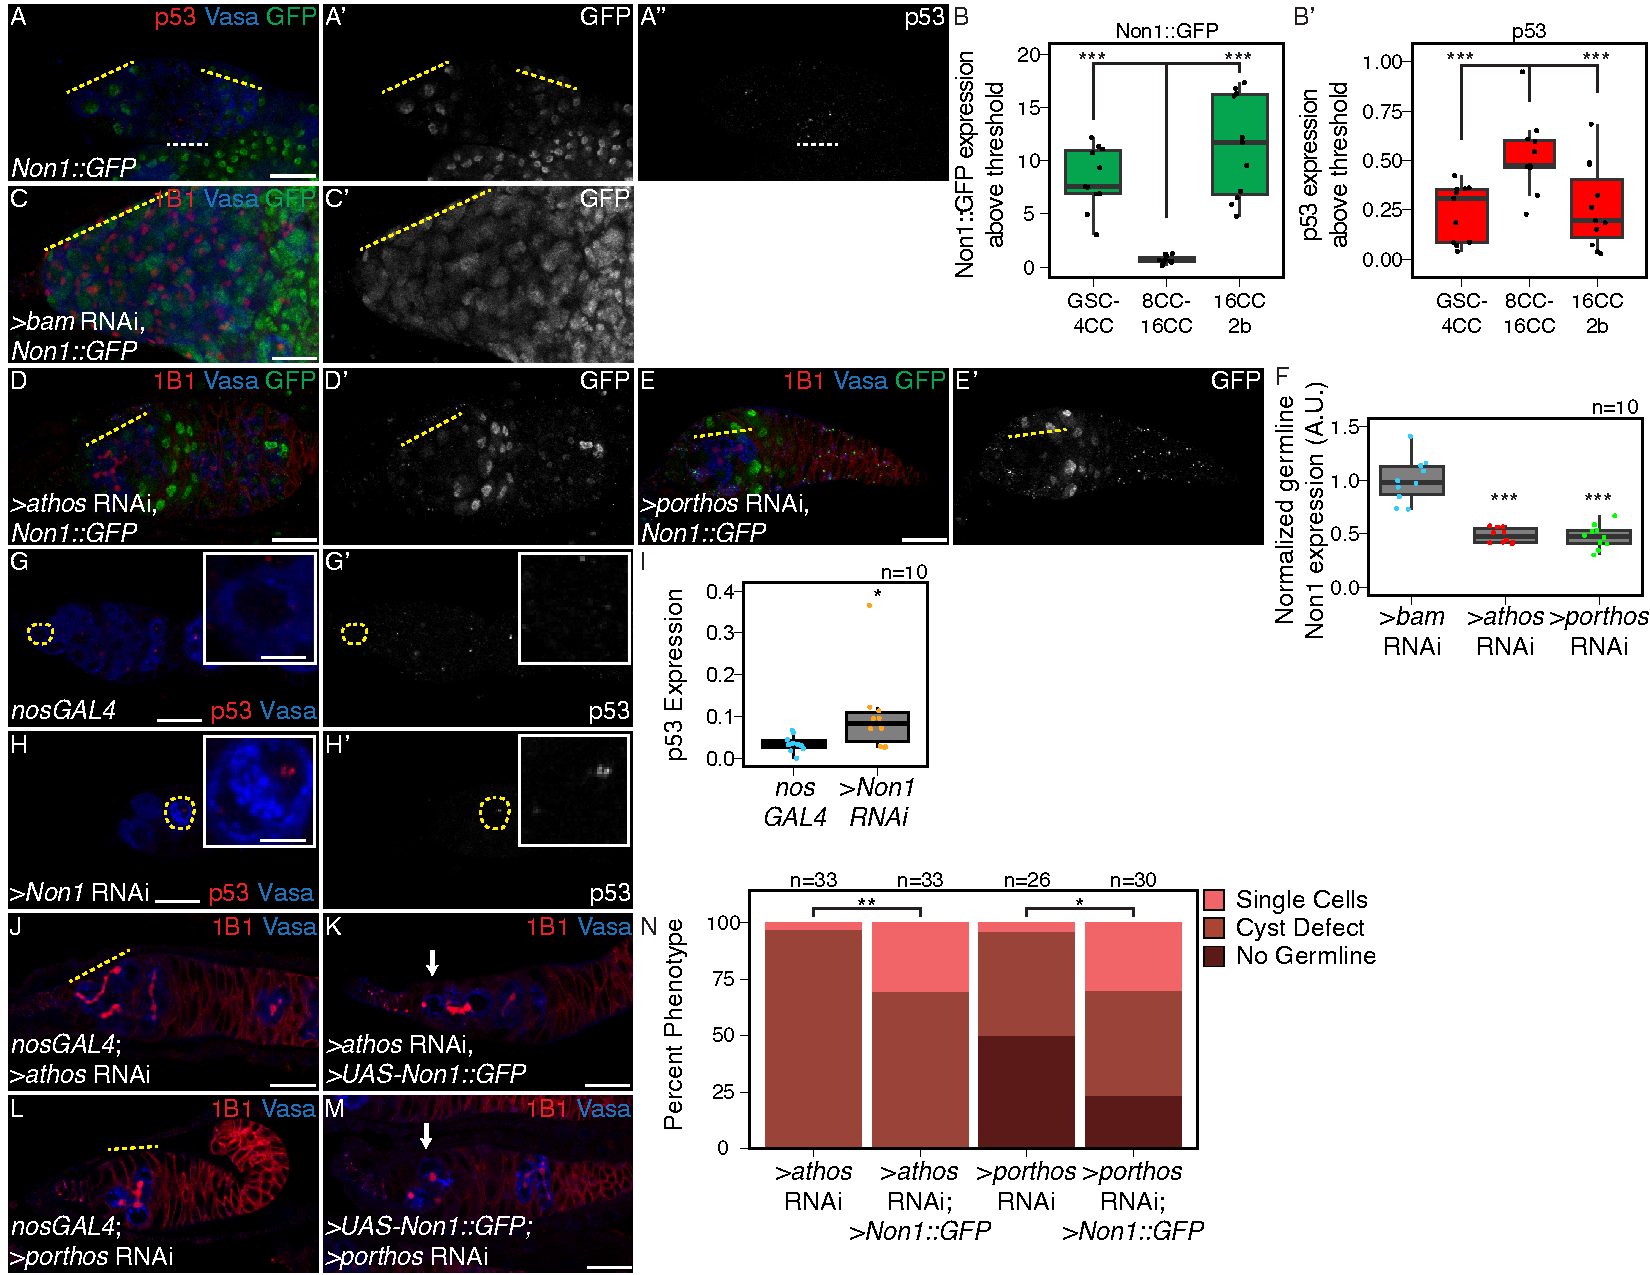
\includegraphics[width=7 in,height=5.409091 in]{./figure/Ribosome Biogenesis/Ribosome Biogenesis 5S} 

}

\caption[\textbf{Non1 and p53 are inversely expressed, related to Figure 2.9.}]{\textbf{Non1 and p53 are inversely expressed, related to Figure 2.9.}}\label{fig:unnamed-chunk-15}
\end{figure}
\setstretch{1.0}

\setlength\parindent{0pt}(\textbf{A-A''}) Confocal images of ovarioles expressing Non1::GFP stained for p53 (red, right grayscale), Vasa (blue), and Non1::GFP (green, left grayscale). (\textbf{B-B'}) Quantifications of staining, (\textbf{B}) peak Non1 expression in control ovaries occurs in GSC-4 cell cyst stages and 16-cell cyst-region 2b stages where (\textbf{B'}) p53 expression is low. (\textbf{C-E'}) Confocal images of germline (\textbf{C-C'}) \emph{bam} RNAi, (\textbf{D-D'}) germline \emph{athos} RNAi, or (\textbf{E-E'}) germline \emph{porthos} RNAi germaria stained for 1B1 (red), \emph{Non1::GFP} (green, greyscale), and Vasa (blue). (\textbf{F}) Quantification of Non1:GFP expression in germline \emph{athos, or porthos} RNAi compared to germline \emph{bam} RNAi as a developmental control demonstrates there is significantly lower Non1::GFP expression in \emph{athos, or porthos} RNAi compared to \emph{bam} RNAi (n=10 germaria per genotype, Welch's t-test, *** = p\textless0.001) (\textbf{G-H'}) Confocal images of (\textbf{G-G'}) \emph{nosGAL4}, driver control and germline (\textbf{H-H'}) \emph{Non1} RNAi germaria stained for p53 (red, grayscale) and Vasa (blue). (\textbf{I}) Quantification of p53 punctate area above cutoff are markedly brighter in the germline of \emph{Non1} RNAi depleted ovaries compared to the control (n=10 germaria per genotype, Welch's t-test, * = p\textless0.05). Cells highlighted by a dashed yellow circle represent cells shown in the inset. (\textbf{J-M}) Confocal images of germaria stained for 1B1 (red, grayscale), and Vasa (blue) in (\textbf{J}) \emph{athos} germline RNAi exhibiting stem-cyst phenotype (yellow dashed line) and (\textbf{K}) \emph{athos} germline RNAi with \emph{Non1} overexpression exhibiting single cells (arrow), (\textbf{L}) \emph{porthos} germline RNAi exhibiting stem-cyst phenotype (yellow dashed line) and (\textbf{M}) \emph{porthos} germline RNAi with \emph{Non1} overexpression exhibiting single cells (arrow). (\textbf{N}) Phenotypic quantification of germline \emph{athos} RNAi or \emph{porthos} RNAi with \emph{Non1} overexpression demonstrates a significant alleviation of the stem-cyst phenotype compared to germline \emph{athos} or \emph{porthos} RNAi alone (n=26-33 germaria per genotype, df=2, Fisher's exact test, * = p\textless{} 0.05, ** = p\textless{} 0.01). Scale bar for main images is 15 micron, scale bar for insets is 3.75 micron.

\setstretch{2.0}

\textbf{\\
}

\hypertarget{aramis-regulated-targets-contain-a-top-motif-in-their-5utr}{%
\subsection{Aramis-regulated targets contain a TOP motif in their 5'UTR}\label{aramis-regulated-targets-contain-a-top-motif-in-their-5utr}}

We next asked how \emph{aramis} and efficient ribosome biogenesis promote the translation of a subset of mRNAs, including \emph{Non1}, to regulate GSC differentiation. We hypothesized that the 87 mRNA targets share a property that make them sensitive to rRNA and ribosome levels. To identify shared characteristics, we performed \emph{de novo} motif discovery of target genes compared to non-target genes ({\textbf{???}}) and identified a polypyrimidine motif in the 5'UTRs of most target genes (UCUUU; E-value: 6.6e\textsuperscript{-094}). This motif resembles the previously described TOP motif at the 5' end of mammalian transcripts ({\textbf{???}}; {\textbf{???}}). Although the existence of TOP-containing mRNAs in \emph{Drosophila} has been speculated, to our knowledge their presence has not been explicitly demonstrated ({\textbf{???}}; {\textbf{???}}). This observation motivated us to precisely determine the 5' end of transcripts, so we analyzed previously published Cap Analysis of Gene Expression sequencing (CAGE-seq) data that had determined transcription start sites (TSS) in total mRNA from the ovary (\textbf{Figure 6A}) ({\textbf{???}}; {\textbf{???}}; {\textbf{???}}). Of the 87 target genes, 76 had sufficient expression in the CAGE-seq dataset to define their TSS. We performed motif discovery using the CAGE-seq data and found that 72 of 76 Aramis-regulated mRNAs have a polypyrimidine motif that starts within the first 50 nt of their TSS (\textbf{Figure 2.11B-C}). In mammals, it was previously thought that the canonical TOP motif begins with an invariant 'C' ({\textbf{???}}; {\textbf{???}}). However, systematic characterization of the sequence required in order for an mRNA to be regulated as a TOP containing mRNA revealed that TOP mRNAs can start with either a 'C' or a 'U' ({\textbf{???}}). Thus, mRNAs whose efficient translation is dependent on \emph{aramis} share a terminal polypyrimidine-rich motif in their 5'UTR that resembles a TOP motif.

In vertebrates, most canonical TOP-regulated mRNAs encode ribosomal proteins and translation initiation factors that are coordinately upregulated in response to growth cues mediated by the Target of Rapamycin (TOR) pathway and the TOR complex 1 (mTORC1) ({\textbf{???}}; {\textbf{???}}; {\textbf{???}}; {\textbf{???}}; {\textbf{???}}) Indeed, 76 of the 87 Aramis targets were ribosomal proteins, and 9 were known or putative translation factors, consistent with TOP-containing RNAs in vertebrates (\textbf{Figure 2.7C, Supplemental Table 2.6}). To determine if the putative TOP motifs that we identified are sensitive to TORC1 activity, we designed ``TOP reporter'' constructs. Specifically, the germline-specific \emph{nanos} promoter was employed to drive expression of an mRNA with 1) the 5'UTR of the \emph{aramis} target \emph{RpL30}, which contains a putative TOP motif, 2) the coding sequence for a GFP-HA fusion protein and 3) a 3'UTR (K10) that is not translationally repressed ({\textbf{???}}; {\textbf{???}}), referred to as the WT-TOP reporter (\textbf{Figure 2.11D}). As a control, we created a construct in which the polypyrimidine sequence was mutated to a polypurine sequence referred to as the Mut-TOP reporter (\textbf{Figure 2.11D}).

In \emph{Drosophila}, TORC1 activity increases during meiotic cyst stages ({\textbf{???}}; {\textbf{???}}). We found that the WT-TOP reporter displayed peak expression in 8-cell cysts, whereas the Mutant-TOP reporter did not \textbf{(Figure 2.11E-F'')}, suggesting that the WT-TOP reporter is sensitive to TORC1 activity. Moreover, depletion of \emph{Nitrogen permease regulator-like 3} (\emph{Nprl3}), an inhibitor of TORC1 ({\textbf{???}}), led to a significant increase in expression of the WT-TOP reporter but not the Mutant-TOP reporter \textbf{(Figure 2.12A-E)}. Additionally, to attenuate TORC1 activity, we depleted \emph{raptor}, one of the subunits of the TORC1 complex ({\textbf{???}}; {\textbf{???}}). Here we found that the WT-TOP reporter had a significant decrease in reporter expression while the Mutant-TOP reporter did not show a decrease in expression \textbf{(Figure 2.12F-J)}. Taken together, our data suggest that Aramis-target transcripts contain TOP motifs that are sensitive to TORC1 activity. However, we note that our TOP reporter did not recapitulate the pattern of Non1::GFP expression, suggesting that Non1 may have additional regulators that modulate its protein levels in the cyst stages.
\begin{figure}

{\centering 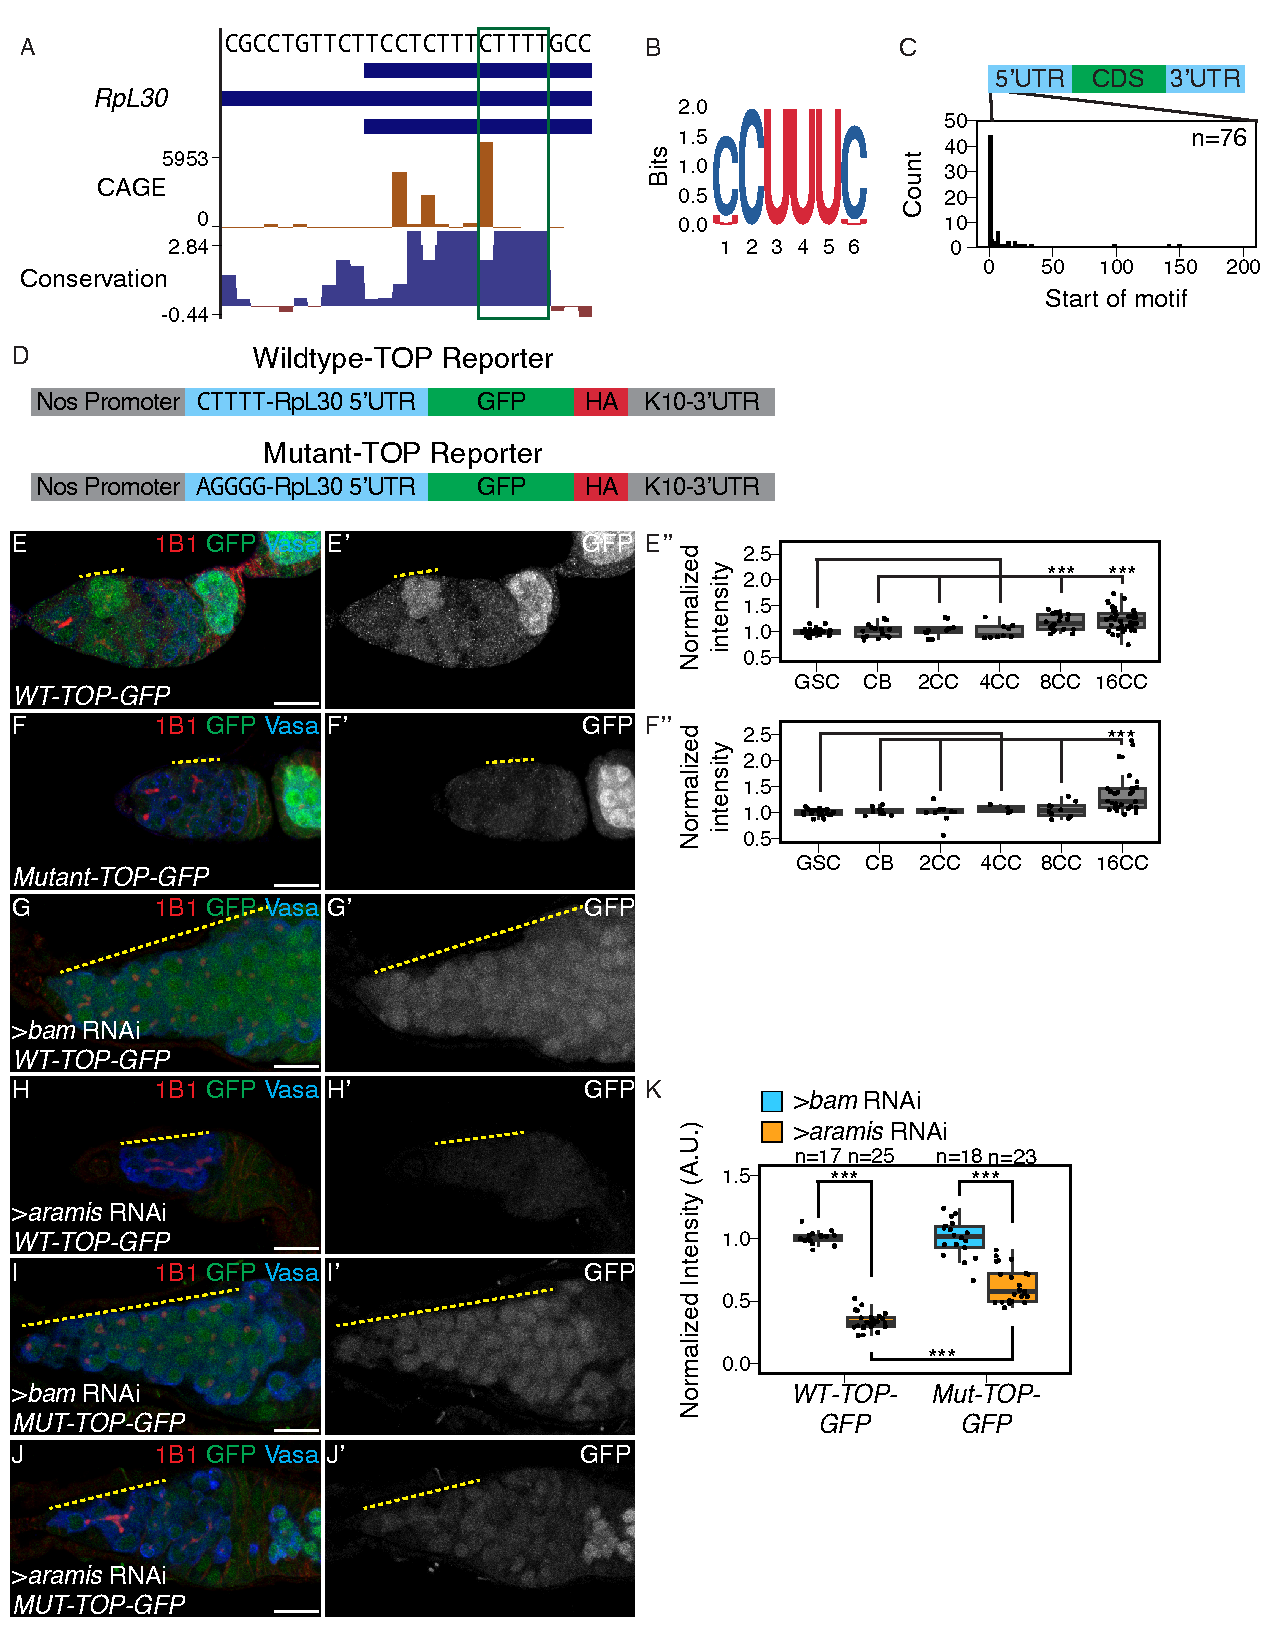
\includegraphics[width=6.5 in,height=8.9375 in]{./figure/Ribosome Biogenesis/Ribosome Biogenesis 6} 

}

\caption[\textbf{Aramis regulated mRNAs contain a TOP motif.}]{\textbf{Aramis regulated mRNAs contain a TOP motif.}}\label{fig:unnamed-chunk-16}
\end{figure}
\setstretch{1.0}

\setlength\parindent{0pt}(\textbf{A}) Genome browser tract of \emph{RpL30} locus in ovary CAGE-seq data showing the proportion of transcripts that are produced from a given TSS (orange). Predominant TSSs are shown in orange and putative TOP motif indicated with a green box. The bottom blue and red graph represents sequence conservation of the locus across \emph{Diptera}. The dominant TSS initiates with a canonical TOP motif. (\textbf{B}) Sequence logo generated from \emph{de novo} motif discovery on the first 200 bases downstream of CAGE derived TSSs of \emph{aramis} translation target genes resembles a canonical TOP motif. (\textbf{C}) Histogram representing the location of the first 5-mer polypyrimidine sequence from each CAGE based TSS of \emph{aramis} translation target genes demonstrates that the TOP motifs occur proximal to the TSS (n=76 targets). (\textbf{D}) Diagram of the \emph{WT} and \emph{Mut-TOP-GFP} reporter constructs indicating the TOP sequence that is mutated by transversion in the Mutant reporter (blue). (\textbf{E-F''}) Confocal images and quantifications of (\textbf{E-E'}) \emph{WT-TOP-GFP} and (\textbf{F-F'}) \emph{Mut-TOP-GFP} reporter expression stained for 1B1 (red), GFP (green, grayscale), and Vasa (blue). Yellow dotted-line marks increased reporter expression in 8-cell cysts of \emph{WT-TOP-GFP} but not in \emph{Mut-TOP-GFP}. Reporter expression was quantified over germline development for (\textbf{E''}) \emph{WT-TOP-GFP} and (\textbf{F''}) \emph{Mut-TOP-GFP} reporter expression and normalized to expression in the GSC reveals dynamic expression based on the presence of a TOP motif. (\textbf{G-H'}) Confocal images of \emph{WT-TOP-GFP} reporter ovarioles showing 1B1 (red), GFP (green, grayscale), and Vasa (blue) in (\textbf{G-G'}) \emph{bam} germline depletion as a developmental control and (\textbf{H-H'}) \emph{aramis} germline depleted ovaries. Yellow dotted lines indicate germline. (\textbf{I-J'}) Confocal images of \emph{Mut-TOP-GFP} reporter expression showing 1B1 (red), GFP (green, grayscale), and Vasa (blue) in (\textbf{I-I'}) \emph{bam} RNAi and (\textbf{J-J'}) \emph{aramis} germline RNAi. Yellow dotted lines indicate germline. (\textbf{K}) A.U. quantification of WT and Mutant TOP reporter expression in undifferentiated daughter cells in \emph{bam} RNAi compared \emph{aramis} RNAi demonstrates that the \emph{WT-TOP-GFP} reporter shows significantly lower expression in \emph{aramis} RNAi than the \emph{Mut-TOP-GFP} relative to the expression of the respective reporters in \emph{bam} RNAi indicating that the presence of a TOP motif sensitizes transcripts to regulation (n=17-25 germaria per genotype, with Welch's t-test *** = p\textless0.001). Scale bar for all images is 15 micron.

\setstretch{2.0}

\textbf{\\
}

TOP mRNAs show increased translation in response to TOR signaling, leading to increased ribosome biogenesis ({\textbf{???}}; {\textbf{???}}; {\textbf{???}}; {\textbf{???}}). However, to our knowledge, whether reduced ribosome biogenesis can coordinately diminish the translation of TOP mRNAs to balance and lower ribosome protein production and thus balance the levels of the distinct components needed for full ribosome assembly is not known. To address this question, we crossed the transgenic flies carrying the WT-TOP reporter and Mutant-TOP reporter into \emph{bam} and \emph{aramis}, \emph{athos}, and \emph{porthos} germline RNAi backgrounds. We found that the expression from the WT-TOP reporter was reduced by 2.9-fold in the germline of \emph{aramis} RNAi ovaries compared to \emph{bam} RNAi ovaries \textbf{(Figure 2.11F-G, J)}. In contrast, the Mutant-TOP reporter was only reduced by 1.6-fold in the germline of \emph{aramis} RNAi ovaries compared to \emph{bam} RNAi ovaries \textbf{(Figure 2.11H-J)}. We observed the same trend for \emph{athos} and \emph{porthos} (\textbf{Figure 2.12K-Q}). This suggests that the TOP motif-containing mRNAs are sensitive to ribosome biogenesis.
\begin{figure}

{\centering \includegraphics[width=6.5 in,height=8.9375 in]{./figure/Ribosome Biogenesis/Ribosome Biogenesis 6S} 

}

\caption[\textbf{TORC1 activity, Athos, and Porthos, regulate TOP expression in the germarium, related to Figure 2.11.}]{\textbf{TORC1 activity, Athos, and Porthos, regulate TOP expression in the germarium, related to Figure 2.11.}}\label{fig:unnamed-chunk-17}
\end{figure}
\setlength\parindent{0pt}(\textbf{A-B}) Confocal images of \emph{WT-TOP} reporter expression stained for 1B1 (red), GFP (green), and Vasa (blue) in (\textbf{A}) \emph{nosGAL4}, driver control ovaries and (\textbf{B}) ovaries depleted of \emph{Nprl3} in the germline. (\textbf{C-D}) Confocal images of \emph{Mut-TOP-GFP} reporter expression stained for 1B1 (red), GFP (green, grayscale), and Vasa (blue) in (\textbf{C}) \emph{nosGAL4}, driver control ovaries and (\textbf{D}) ovaries depleted of \emph{Nprl3} in the germline. (\textbf{E}) A.U. quantification of WT and Mutant TOP reporter expression in GSCs of \emph{nosGAL4}, driver control ovaries and GSCs of \emph{Nprl3} germline depleted ovaries normalized to Vasa expression indicate that the relative expression of the \emph{WT-TOP-GFP} reporter is higher than the \emph{Mut-TOP-GFP} reporter (n=9-11 germaria per genotype, Welch's t-test, * = p\textless0.05, ** = p\textless0.01, *** = p\textless0.001). (\textbf{F-G}) Confocal images of \emph{WT-TOP} reporter expression stained for 1B1 (red), GFP (green), and Vasa (blue) in (\textbf{F}) \emph{nosGAL4}, driver control ovaries and (\textbf{G}) ovaries depleted of \emph{raptor} in the germline. (\textbf{H-I}) Confocal images of \emph{Mut-TOP-GFP} reporter expression stained for 1B1 (red), GFP (green), and Vasa (blue) in (\textbf{H}) \emph{nosGAL4}, driver control ovaries and (\textbf{I}) ovaries depleted of \emph{raptor} in the germline. (\textbf{J}) A.U. quantification of WT and Mutant TOP reporter expression in GSCs of \emph{nosGAL4}, driver control ovaries and GSCs of \emph{raptor} germline depleted ovaries normalized to Vasa expression indicate that the relative expression of the \emph{WT-TOP-GFP} reporter is lower than the \emph{Mut-TOP-GFP} reporter (n=10 germaria per genotype, Welch's t-test, * = p\textless0.05, ** = p\textless0.01). (\textbf{K-M'}) Confocal images of \emph{WT-TOP-GFP} reporter ovarioles showing 1B1 (red), GFP (green, grayscale), and Vasa (blue) in (\textbf{K-K'}) \emph{bam} germline depletion as a developmental control, (\textbf{L-L'}) \emph{athos} germline depleted ovaries, and (\textbf{M-M'}) \emph{porthos} germline depleted ovaries. Yellow dotted lines indicate germline. (\textbf{N-P'}) Confocal images of \emph{Mut-TOP-GFP} reporter expression showing 1B1 (red), GFP (green, grayscale), and Vasa (blue) in (\textbf{N-N'}) \emph{bam} RNAi, (\textbf{O-O'}) \emph{athos} germline RNAi, and (\textbf{P-P'}) \emph{porthos} germline depleted ovaries. Yellow dotted lines indicate germline. (\textbf{Q}) A.U. quantification of WT and Mutant TOP reporter expression in undifferentiated daughter cells in \emph{bam} RNAi compared \emph{athos} or \emph{porthos} RNAi demonstrates that the \emph{WT-TOP-GFP} reporter shows significantly lower expression in \emph{athos} and \emph{porthos} RNAi than the \emph{Mut-TOP-GFP} relative to the expression of the respective reporters in \emph{bam} RNAi indicating that the presence of a TOP motif sensitizes transcripts to regulation (n=17-25 germaria per genotype, with Welch's t-test with , ** = p\textless0.01, *** = p\textless0.001). Scale bar for images is 15 micron.

\textbf{\\
}

\hypertarget{larp-binds-top-sequences-in-drosophila}{%
\subsection{\texorpdfstring{Larp binds TOP sequences in \emph{Drosophila}}{Larp binds TOP sequences in Drosophila}}\label{larp-binds-top-sequences-in-drosophila}}

Next, we sought to determine how TOP-containing mRNAs are regulated downstream of Aramis. In mammalian cells, Larp1 is a critical negative regulator of TOP-containing RNAs during nutrient deprivation ({\textbf{???}}; {\textbf{???}}; {\textbf{???}}; {\textbf{???}}; {\textbf{???}}). Therefore, we hypothesized that \emph{Drosophila} Larp reduces the translation of TOP-containing mRNAs when rRNA biogenesis is reduced upon loss of \emph{aramis}. First, using an available gene-trap line in which endogenous Larp is tagged with GFP and 3XFLAG, we confirmed that Larp was robustly expressed throughout all stages of oogenesis including in GSCs \textbf{(Figure 2.14A-A')}.

Next, we performed electrophoretic mobility shift assays (EMSA) to examine protein-RNA interactions with purified \emph{Drosophila} Larp-DM15, the conserved domain that binds to TOP sequences in vertebrates ({\textbf{???}}). As probes, we utilized capped 42-nt RNAs corresponding to the 5'UTRs of \emph{RpL30} and \emph{Non1}, including their respective TOP sequences. We observed a gel shift with these RNA oligos in the presence of increasing concentrations of Larp-DM15 \textbf{(Figure 2.13A-A', Figure 2.14B)}, and this shift was abrogated when the TOP sequences were mutated to purines \textbf{(Figure 2.14C-C').} To determine if Larp interacts with TOP-containing mRNAs \emph{in vivo}, we immunopurified Larp::GFP::3XFLAG from the ovaries of the gene-trap line and performed RNA-seq (\textbf{Figure 2.14D}). We uncovered 156 mRNAs that were bound to Larp, and 84 of these were among the 87 \emph{aramis} translationally regulated targets, including \emph{Non1}, \emph{RpL30}, and \emph{RpS2} (\textbf{Figure 2.13B-C, Supplemental Table 2.7}). Thus, \emph{Drosophila} Larp binds to TOP sequences \emph{in vitro} and TOP-containing mRNAs \emph{in vivo}.
\begin{figure}

{\centering \includegraphics[width=6.5 in,height=8.9375 in]{./figure/Ribosome Biogenesis/Ribosome Biogenesis 7} 

}

\caption[\textbf{Larp binds to TOP mRNAs and binding is regulated by Aramis.}]{\textbf{Larp binds to TOP mRNAs and binding is regulated by Aramis.}}\label{fig:unnamed-chunk-18}
\end{figure}
\setstretch{1.0}

\setlength\parindent{0pt}(\textbf{A-A'}) EMSA of Larp-DM15 and the leading 42 nucleotides of (\textbf{A}) \emph{RpL30} and (\textbf{A'}) \emph{Non1} with increasing concentrations of Larp-DM15 from left to right indicates that both RNAs bind to Larp-DM15. (\textbf{B}) Volcano plot of mRNAs in Larp::GFP::3XFLAG IP compared to input. Blue points represent mRNAs significantly enriched in Larp::GFP::3XFLAG compared to input, but not enriched in an IgG control compared to input. (\textbf{C}) Venn diagram of overlapping Larp IP targets and \emph{aramis} RNAi polysome seq targets indicates that Larp physically associates with mRNAs that are translationally downregulated in germline \emph{aramis} RNAi (p \textless{} 0.001, Hypergeometric Test). (\textbf{D}) Bar plot representing the fold enrichment of mRNAs from Larp RNA IP in germline \emph{aramis} RNAi relative to matched \emph{bam} RNAi ovaries as a developmental control measured with qPCR (n=3, * = p\textless0.5, ** = p\textless0.01, NS = nonsignificant, One-sample t-test, mu=1) indicates that more of two \emph{aramis} translation targets \emph{Non1} and \emph{RpL30} are bound by Larp in \emph{aramis} RNAi. (\textbf{E-F''}) Confocal images of (\textbf{E-E''}) \emph{nosGAL4}, driver control and (\textbf{F-F''}) ovaries overexpressing the DM15 region of Larp in the germline ovaries stained for 1B1 (red, left grayscale), Vasa (blue), and Larp-DM15::GFP (green, right grayscale). Overexpression of Larp results in an accumulation of extended 1B1 structures (highlighted with a dotted yellow line), marking interconnected cells when Larp-DM15 is overexpressed compared to \emph{nosGAL4}, driver control ovaries. (\textbf{G}) In conditions with normal ribosome biogenesis Non1 is efficiently translated, downregulating p53 levels allowing for progression through the cell cycle. When ribosome biogenesis is perturbed Non1 is not translated to sufficient levels, resulting in the accumulation of p53 and cell cycle arrest. Dotted lines indicate indirect affects. Scale bar for all images is 15 micron.

\setstretch{2.0}

\textbf{\\
}

To test our hypothesis that \emph{Drosophila} Larp inhibits the translation of TOP-containing mRNAs upon loss of \emph{aramis}, we immunopurified Larp::GFP::3XFLAG from germline \emph{bam} RNAi ovaries and germline \emph{aramis} RNAi ovaries. Larp protein is not expressed at higher levels in \emph{aramis} RNAi compared to developmental control \emph{bam} RNAi (\textbf{Figure 2.14E-G}). Larp protein is also not expressed at higher levels in \emph{bam} RNAi; \emph{aramis} RNAi germline knockdown compared to \emph{bam} RNAi as a control (\textbf{Figure 2.14H-I}). We found that Larp binding to \emph{aramis} target mRNAs \emph{Non1} and \emph{RpL30} was increased in \emph{aramis} RNAi ovaries compared to \emph{bam} RNAi ovaries (\textbf{Figure 2.13D, Figure 2.14J}). In contrast, a non-target mRNA that does not contain a TOP motif, \emph{alpha-tubulin} mRNA, did not have a significant increase in binding to Larp in \emph{aramis} RNAi ovaries compared to \emph{bam} RNAi ovaries. Overall, these data suggest that reduced rRNA biogenesis upon loss of \emph{aramis} increases Larp binding to the TOP-containing mRNAs \emph{Non1} and \emph{RpL30}.

If loss of \emph{aramis} inhibits the translation of TOP-containing mRNAs due to increased binding of Larp to its targets, then overexpression of Larp would be expected to phenocopy germline depletion of \emph{aramis}. Unphosphorylated Larp binds to TOP motifs more efficiently, but the precise phosphorylation sites of \emph{Drosophila} Larp, to our knowledge, are currently unknown ({\textbf{???}}). To circumvent this issue, we overexpressed the DM15 domain of Larp which we showed binds the \emph{RpL30} and \emph{Non1} TOP motifs \emph{in vitro} (\textbf{Figure 2.13A-A'}), and, based on homology to mammalian Larp1, lacks majority of the putative phosphorylation sites ({\textbf{???}}; {\textbf{???}}; {\textbf{???}}). We found that overexpression of a Larp-DM15::GFP fusion in the germline resulted in fusome-like structures extending from the niche (\textbf{Figure 2.13E-F'})\textbf{.} Additionally, ovaries overexpressing Larp-DM15 had 32-cell egg chambers, which were not observed in control ovaries (\textbf{Figure 2.14K-K'}). The presence of 32-cell egg chambers is emblematic of cytokinesis defects that occur during early oogenesis ({\textbf{???}}; {\textbf{???}}; {\textbf{???}}). Our findings indicate that these cells are delayed in cytokinesis and that over expression of Larp partially phenocopies depletion of \emph{aramis}.
\begin{figure}

{\centering \includegraphics[width=6.5 in,height=8.9375 in]{./figure/Ribosome Biogenesis/Ribosome Biogenesis 7S} 

}

\caption[\textbf{Larp binds specifically to TOP containing mRNAs and regulates cytokinesis, related to Figure 2.13.}]{\textbf{Larp binds specifically to TOP containing mRNAs and regulates cytokinesis, related to Figure 2.13.}}\label{fig:unnamed-chunk-19}
\end{figure}
\setstretch{1.0}

\setlength\parindent{0pt}(\textbf{A-A'}) Confocal images of germaria stained for 1B1 (red), Vasa (blue), and \emph{Larp GFP-3XFLAG} (green, grayscale) indicates Larp is expressed throughout early oogenesis. (\textbf{B}) Quantification of EMSAs and summary of K\textsubscript{d} of the protein-RNA interactions. (\textbf{C-C'}) EMSA of Larp-DM15 and the leading 42 nucleotides of (\textbf{B}) \emph{RpL30} and (\textbf{B'}) \emph{Non1} with their TOP sequence mutated to purines as a negative control with increasing concentrations of Larp-DM15 from left to right indicates that Larp-DM15 requires a leading TOP sequence for its binding. (\textbf{D}) Western of representative IP of Larp::GFP::3XFLAG from ovary tissue used for RNA IP-seq. (\textbf{E-F'}) Confocal images of Larp::GFP::3XFLAG reporter expression stained for 1B1 (red), GFP (green, grayscale), and Vasa (blue) in (\textbf{E-E'}) \emph{bam} and (\textbf{F-F'}) \emph{aramis}-depleted germaria. (\textbf{G}) A.U. quantification of Larp::GFP::3XFLAG reporter expression in the germline of \emph{bam} RNAi and \emph{aramis} RNAi normalized to germline Vasa intensity demonstrates that the germline expression of Larp is not elevated in \emph{aramis} germline RNAi compared to \emph{bam} germline RNAi as a developmental control (n=10, NS = p\textgreater0.05, Welch's t-test). (\textbf{H-H'}) Confocal images of Larp::GFP::3XFLAG reporter expression stained for 1B1 (red), GFP (green), and Vasa (blue) in (\textbf{H}) \emph{bam} and (\textbf{H'}) \emph{bam}; \emph{aramis}-depleted germaria. (\textbf{I}) A.U. quantification of Larp::GFP::3XFLAG reporter expression in the germline of \emph{bam} RNAi and \emph{bam} RNAi ; \emph{aramis} RNAi demonstrates that the germline expression of Larp normalized to somatic Larp expression is not elevated in \emph{bam}; \emph{aramis} germline RNAi compared to \emph{bam} germline RNAi as a developmental control (n=10, NS = p\textgreater0.05, Welch's t-test). (\textbf{J}) Western of representative IP of Larp::GFP::3XFLAG from ovary tissue used for RNA IP qPCR. (\textbf{K-K'}) Confocal images of (\textbf{K}) \emph{nosGAL4}, driver control and (\textbf{K'}) ovaries overexpressing the DM15 region of Larp in the germline ovaries stained for DAPI (green) and Vasa (blue). Overexpression of Larp-DM15 results in the production of 32-cell egg chambers which indicates it causes a cytokinesis defect. Scale bar for all images is 15 micron.

\setstretch{2.0}

\textbf{\\
}

\hypertarget{discussion}{%
\section{Discussion}\label{discussion}}

During \emph{Drosophila} oogenesis, efficient ribosome biogenesis is required in the germline for proper GSC cytokinesis and differentiation. The outstanding questions that needed to be addressed were: 1) Why does disrupted ribosome biogenesis impair GSC abscission and differentiation? And 2) How does the GSC monitor and couple ribosome abundance to differentiation? Our results suggest that a germline ribosome biogenesis defect stalls the cell cycle, resulting a loss of differentiation and the formation of stem-cysts. We discovered that proper ribosome biogenesis is monitored through a translation control module that allows for co-regulation of ribosomal proteins and a p53 repressor. Loss of \emph{aramis}, \emph{athos} and \emph{porthos} reduces ribosome biogenesis and inhibits translation of a p53 repressor, leading to p53 stabilization, cell cycle arrest and loss of stem cell differentiation (\textbf{Figure 2.13G}).

\hypertarget{aramis-athos-and-porthos-are-required-for-efficient-ribosome-biogenesis-in-drosophila}{%
\subsection{\texorpdfstring{Aramis, Athos, and Porthos are required for efficient ribosome biogenesis in \emph{Drosophila}}{Aramis, Athos, and Porthos are required for efficient ribosome biogenesis in Drosophila}}\label{aramis-athos-and-porthos-are-required-for-efficient-ribosome-biogenesis-in-drosophila}}

We provide evidence that Aramis, Athos and Porthos play a role in ribosome biogenesis in \emph{Drosophila}, similar to their orthologs in yeast ({\textbf{???}}; {\textbf{???}}; {\textbf{???}}; {\textbf{???}}) and mammals ({\textbf{???}}; {\textbf{???}}; {\textbf{???}}). Their role in ribosome biogenesis is likely a direct function of these helicases as they physically interact with precursor rRNA. In yeast, Rok1, the ortholog of Aramis, binds to several sites on pre-rRNA, predominantly in the 18S region ({\textbf{???}}; {\textbf{???}}; {\textbf{???}}). This is consistent with the small subunit ribosome biogenesis defect we observe upon loss of \emph{aramis} in \emph{Drosophila}. Rrp3, the yeast ortholog of Porthos, promotes proper cleavage of pre-rRNA and is required for proper 18S rRNA production ({\textbf{???}}; {\textbf{???}}). DDX47, the mammalian ortholog of Porthos, binds to early rRNA precursors as well as proteins involved in ribosome biogenesis ({\textbf{???}}). Consistent with these findings, we find that Aramis and Porthos promote 40S ribosome biogenesis. DHX33, the mammalian ortholog of Athos, has been implicated in facilitating rRNA synthesis ({\textbf{???}}). In contrast, we find that Athos promotes 60S ribosome biogenesis by directly interacting with rRNA. However, we cannot exclude the possibility that Athos also affects transcription of rRNA in \emph{Drosophila} as it does in mammals ({\textbf{???}}). Overall, we find that each mammalian ortholog of Aramis, Athos, and Porthos has consistent ribosome subunit defects, suggesting that the function of these helicases is conserved from flies to mammals. Intriguingly, DDX52 (Aramis) is one of the 15 genes deleted in 17q12 syndrome ({\textbf{???}}). 17q12 syndrome results in delayed development, intellectual disability, and, more rarely, underdevelopment of organs such as the uterus ({\textbf{???}}; {\textbf{???}}). Our finding that Aramis disrupts stem cell differentiation could explain some of the poorly understood defects in 17q12 syndrome.

\hypertarget{ribosome-biogenesis-defects-leads-to-cell-cycle-defects-mediated-by-p53}{%
\subsection{Ribosome biogenesis defects leads to cell cycle defects mediated by p53}\label{ribosome-biogenesis-defects-leads-to-cell-cycle-defects-mediated-by-p53}}

Here we report that three RNA helicases, \emph{aramis}, \emph{athos}, and \emph{porthos,} that promote proper ribosome biogenesis in \emph{Drosophila} are required in the germline for fertility. Loss of \emph{aramis}, \emph{athos}, and \emph{porthos} causes formation of a ``stem-cyst'' and loss of later stage oocytes. Stem-cysts are a characteristic manifestation of ribosome biogenesis deficiency wherein GSCs are unable to complete cytokinesis and fail to express the differentiation factor Bam, which in GSC daughters is initiated at G2 of the cell cycle ({\textbf{???}}; {\textbf{???}}). Our RNA seq and cell cycle analysis indicates that depletion of \emph{aramis} blocks the cell cycle at G1, and that failure to progress to G2 prevents abscission and expression of Bam. Thus, our results suggest that ribosome biogenesis defects in the germline stall the cell cycle, resulting in formation of stem-cysts and sterility.

In most tissues in \emph{Drosophila,} p53 primarily activates apoptosis, however, in the germline p53 is activated during meiosis and does not cause cell death ({\textbf{???}}; Lu et al., 2010). Furthermore, p53 activation in the germline is required for germline repopulation and GSC survival after genetic insult, implicating p53 as a potential cell cycle regulator ({\textbf{???}}; {\textbf{???}}). Our observation that reduction of \emph{p53} partially rescues a stem-cyst defect caused by ribosome deficiency due to germline depletion of \emph{aramis} indicates that the G1 block in GSCs is, in part, mediated by p53 activation. Thus, in \emph{Drosophila} GSCs, p53 blocks the GSC cell cycle and is sensitive to ribosome biogenesis. Furthermore, while overexpression of p53 causes germline death, it is also sufficient to induce the formation of stem-like cysts demonstrating p53 plays a key regulatory role in GSC cell cycle. The developmental upregulation of p53 during GSC differentiation concomitant with lower ribosome levels parallels observations in disease states, such as ribosomopathies ({\textbf{???}}; {\textbf{???}}; {\textbf{???}}; {\textbf{???}}).

We find that p53 levels in GSCs are regulated by the conserved p53 regulator Non1. In mammalian cells, increased free RpS7 protein due to nucleolar stress binds and sequesters a repressor of p53, MDM2, freeing p53, resulting in G1 cell cycle arrest ({\textbf{???}}; {\textbf{???}}). \emph{Drosophila} have no identified homolog to MDM2. It is not fully known how ribosome levels are monitored in \emph{Drosophila} in the absence of MDM2 and how this contributes to cell cycle progression. In \emph{Drosophila,} Non1 levels are high in the GSCs and p53 is low, and reciprocally Non1 levels are low during meiosis, but p53 is expressed. Our finding that loss of Aramis leads to diminished Non1 and elevated p53, and that either loss of p53 or elevated Non1 suppress differentiation defects caused by loss of Aramis, suggests that, in the female germline, Non1 may fulfill the function of Mdm2 by promoting p53 degradation during \emph{Drosophila} oogenesis. While Non1 has been shown to directly interact with p53, how it regulates p53 levels in both humans and \emph{Drosophila} is not known ({\textbf{???}}; {\textbf{???}}). Overall, our data place Non1 downstream of ribosome biogenesis and upstream of p53 in controlling cell cycle progression and GSC differentiation. However, our data do not rule out that Non1 may also act upstream of or in parallel to Aramis.

The vertebrate ortholog of Non1, GTPBP4, also controls p53 levels and is upregulated in some cancers ({\textbf{???}}; {\textbf{???}}; {\textbf{???}}). This suggests that there may be parallel pathways for monitoring ribosome levels via p53 in different tissue types. Unlike \emph{Drosophila} Non1, its ortholog, GTPBP4 has not been identified as a TOP mRNA, so if it similarly acts as a mediator between ribosome biogenesis and the cell cycle it is likely activated in a somewhat different manner ({\textbf{???}}). However, mammalian Larp1 is required for proper cell cycle progression and cytokinesis ({\textbf{???}}; {\textbf{???}}). Excitingly several differentiation and cell cycle regulation genes in mammals are TOP mRNAs regulated by Larp1, including Tumor Protein, Translationally-Controlled 1 (TPT1) and Nucleosome Assembly Protein 1 Like 1 (NAP1L1) ({\textbf{???}}). TPT1 is a cancer associated factor that has been implicated in activating pluripotency ({\textbf{???}}). Similarly, NAP1L1, a nucleosome assembly protein, is required to maintain proper cell cycle control as loss of NAP1L1 results in cell cycle exit and premature differentiation ({\textbf{???}}). Overall, although the specific targets of Larp1 in mammals may differ from those in \emph{Drosophila}, the mechanism by which Larp modulates cell cycle and differentiation may be conserved.

\hypertarget{ribosome-biogenesis-defects-leads-to-repression-of-top-containing-mrna}{%
\subsection{Ribosome biogenesis defects leads to repression of TOP-containing mRNA}\label{ribosome-biogenesis-defects-leads-to-repression-of-top-containing-mrna}}

TOP-containing mRNAs are known to be coregulated to coordinate ribosome production in response to nutrition or other environmental cues ({\textbf{???}}; {\textbf{???}}; {\textbf{???}}). Surprisingly, our observation that loss of \emph{aramis} reduces translation, albeit indirectly via regulation of ribosome biogenesis, of a cohort of TOP-containing mRNAs, including Non1, suggests that the TOP motif also sensitizes their translation to lowered levels of ribosome biogenesis. This notion is supported by TOP reporter assays demonstrating that reduced translation upon loss of \emph{aramis} requires the TOP motif. We hypothesize that limiting TOP mRNA translation lowers ribosomal protein production to maintain a balance with reduced rRNA production. This feedback mechanism would prevent the production of excess ribosomal proteins that cannot be integrated into ribosomes and the ensuing harmful aggregates ({\textbf{???}}). Additionally, it would coordinate rRNA production and ribosomal protein translation during normal germline development, where it is known that the level of ribosome biogenesis and of global translation are dynamic ({\textbf{???}}; {\textbf{???}}; {\textbf{???}}; Blatt et al., 2020).

\hypertarget{larp-transduces-growth-status-to-ribosome-biogenesis-targets}{%
\subsection{Larp transduces growth status to ribosome biogenesis targets}\label{larp-transduces-growth-status-to-ribosome-biogenesis-targets}}

Recent work has shown that the translation and stability of TOP-containing mRNAs are mediated by Larp1 and its phosphorylation ({\textbf{???}}; {\textbf{???}}; {\textbf{???}}). We found that perturbing rRNA production and thus ribosome biogenesis, without directly targeting ribosomal proteins, similarly results in dysregulation of TOP mRNAs. Our data show that \emph{Drosophila} Larp binds the \emph{RpL30} and \emph{Non1} 5'UTR in a TOP-dependent manner \emph{in vitro} and to 97\% of the translation targets we identified \emph{in vivo.} Together these data suggest that rRNA production regulates TOP mRNAs via Larp. Furthermore, the cytokinesis defect caused by overexpression of Larp-DM15 in the germline suggests that Larp regulation could maintain the homeostasis of ribosome biogenesis more broadly by balancing the expression of ribosomal protein production with the rate of other aspects of ribosome biogenesis, such as rRNA processing, during development.

Previous studies indicate that unphosphorylated Larp1 binds to and represses its targets more efficiently than phosphorylated Larp1 ({\textbf{???}}; {\textbf{???}}; {\textbf{???}}). In mammalian systems Larp1 has been shown to be phosphorylated by the TORC1 complex, AKT, and CDK1 ({\textbf{???}}; {\textbf{???}}; {\textbf{???}}). In \emph{Drosophila}, it has been shown that Pink1 can phosphorylates Larp, and the Pink1 dependent phosphorylation sites have been identified in \emph{Drosophila} Larp ({\textbf{???}}). However, to our knowledge, Larp phosphorylation sites have not been systematically catalogued, nor has it been studied if TORC1, AKT, or CDK1 phosphorylate Larp in \emph{Drosophila}. We have demonstrated that expression of our TOP-reporter is dependent on Raptor and TOP-reporter expression is repressed by Nprl3 (\textbf{Figure 2.12A-J}). These results suggest a model where TORC1 either directly or indirectly monitors ribosome biogenesis status by regulating the activity of Larp. Thus, although we do not know the identity of the kinase that phosphorylates Larp in \emph{Drosophila} definitively, we hypothesize that Larp is not phosphorylated upon loss of \emph{aramis, athos} and \emph{porthos}, when ribosome biogenesis is perturbed. We propose that until ribosome biogenesis homeostasis is reached, this kinase will remain inactive, continuously increasing the pool of dephosphorylated Larp. In this scenario, as dephosphorylated Larp accumulates, it begins to bind its targets. Initially, it will bind its highest affinity targets, presumably encoding ribosomal proteins and repress their translation to rebalance ribosomal protein production with rRNA production. Consistent with this model, the TOP motif in \emph{RpL30} is bound by Larp even more tightly with a nearly 9-fold higher affinity compared to the \emph{Non1} TOP site (\textbf{Figure 2.14B}). We propose that such differences in affinity may allow Larp to repress ribosomal protein translation to facilitate cellular homeostasis without immediately causing cell cycle arrest. However, if homeostasis cannot be achieved and sufficient dephosphorylated Larp accumulates, Larp will also bind and repress the translation of lower affinity targets. Repression of Non1 in this manner would result in cell cycle arrest and block differentiation as occurs upon \emph{aramis} depletion.

\hypertarget{ribosome-biogenesis-in-stem-cell-differentiation-and-ribosomopathies}{%
\subsection{Ribosome biogenesis in stem cell differentiation and ribosomopathies}\label{ribosome-biogenesis-in-stem-cell-differentiation-and-ribosomopathies}}

Ribosomopathies arise from defects in ribosomal components or ribosome biogenesis and include a number of diseases such as Diamond-Blackfan anemia, Treacher Collins syndrome, Shwachman-Diamond syndrome, and 5q-myelodysplastic syndrome ({\textbf{???}}; {\textbf{???}}; {\textbf{???}}; {\textbf{???}}; {\textbf{???}}). Despite the ubiquitous requirement for ribosomes and translation, ribosomopathies cause tissue-specific disease ({\textbf{???}}). The underlying mechanisms of tissue specificity remain unresolved.

In this study we demonstrate that loss of helicases involved in rRNA processing lead to perturbed ribosome biogenesis and, ultimately, cell cycle arrest. Given that \emph{Drosophila} germ cells undergo an atypical cell cycle program as a normal part of their development it may be that this underlying cellular program in the germline leads to the tissue-specific symptom of aberrant stem-cyst formation ({\textbf{???}}). This model implies that other tissues would likewise exhibit unique tissue-specific manifestations of ribosomopathies due to their underlying cell state and underscores the need to further explore tissue-specific differentiation programs and development to shed light not only on ribosomopathies but also on other tissue-specific diseases associated with ubiquitous processes. Although it is also possible that phenotypic differences arise from a common molecular cause, our data suggests two sources of potential tissue specificity: 1) tissues express different cohorts of mRNAs, such as \emph{Non1}, that are sensitive to ribosome levels. For example, we find that in \emph{Drosophila} macrophages, RNAs that regulate the metabolic state of macrophages and influence their migration require increased levels of ribosomes for their translation ({\textbf{???}}). 2) p53 activation, as has been previously described, is differentially tolerated in different developing tissues ({\textbf{???}}; {\textbf{???}}; {\textbf{???}}). Together, both mechanisms could begin to explain the tissue-specific nature of ribosomopathies and their link to differentiation.

\textbf{Acknowledgements}

We are grateful to all members of the Rangan and Fuchs labs for their discussion and comments on the manuscript. We also thanks Dr.~Sammons, Dr.~Marlow and Life Science Editors for their thoughts and comments the manuscript Additionally, we thank the Bloomington Stock Center, the Vienna \emph{Drosophila} Resource Center, the BDGP Gene Disruption Project, and Flybase for fly stocks, reagents, and other resources. P.R. is funded by the NIH/NIGMS (R01GM111779-06 and RO1GM135628-01), G.F. is funded by NSF MCB-2047629 and NIH RO3 AI144839, D.E.S. was funded by Marie Curie CIG 334077/IRTIM and the Austrian Science Fund (FWF) grant ASI\_FWF01\_P29638S, and A.B is funded by NIH R01GM116889 and American Cancer Society RSG-17-197-01-RMC.

\textbf{Author Contributions}

Conceptualization, E.T.M., P.B., G.F., and P.R.; Methodology, E.T.M., P.B., G.F., and P.R.; Investigation, E.T.M., P.B., E.N., R.L., S.S., H.Y., T.P., and S.E.; Writing -- Original Draft, E.T.M., D.E.S., and P.R.; Writing -- Review \& Editing, E.T.M., P.B., D.E.S, A.B., G.F., and P.R.; Funding Acquisition, G.F. and P.R.; Visualization, E.T.M., E.N.; Supervision, G.F. and P.R.

\textbf{\\
}

Supplemental Tables can be found along with the original publication here: XXX\\

\textbf{Supplemental Table 2.1. Results of germline helicase RNAi screen on ovariole morphology.}
Results of screen of RNA helicases depleted from the germline. Reported is the majority phenotype from n=50 ovarioles.

\textbf{\\
}

\textbf{Supplemental Table 2.2. Differential expression analysis from RNAseq of ovaries depleted of \emph{aramis} in the germline compared to a developmental control.}
DEseq2 output from RNAseq of ovaries depleted of \emph{aramis} in the germline compared to ovaries depleted of bam in the germline as a developmental control. Sheet 1 (Downregulated Genes) contains genes and corresponding Deseq2 output meeting the cutoffs to be considered downregulated in \emph{aramis} RNAi compared to \emph{bam} RNAi. Sheet 2 (Upregulated Genes) contains genes and corresponding Deseq2 output meeting the cutoffs to be considered upregulated in \emph{aramis} RNAi compared to \emph{bam} RNAi. Sheet 3 (All Genes) contains Deseq2 output for all genes in the dm6 assembly.

\textbf{\\
}

\textbf{Supplemental Table 2.3. Differential expression analysis from RNAseq of ovaries depleted of \emph{bam} and \emph{aramis} in the germline compared to ovaries depleted of \emph{bam} in the germline.}
DEseq2 output from RNAseq of ovaries depleted of \emph{bam} and \emph{aramis} in the germline compared to ovaries depleted of \emph{bam} in the germline as a control. Sheet 1 (Downregulated Genes) contains genes and corresponding DEseq2 output meeting the cutoffs to be considered downregulated in \emph{bam}; \emph{aramis} RNAi compared to \emph{bam} RNAi. Sheet 2 (Upregulated Genes) contains genes and corresponding DEseq2 output meeting the cutoffs to be considered upregulated in \emph{bam}; \emph{aramis} RNAi compared to \emph{bam} RNAi. Sheet 3 (All Genes) contains DEseq2 output for all genes in the dm6 assembly. Sheet 4(BP GO terms - downregulated) contains the output of a Biological Process PANTHER Overrepresentation Test of significantly enriched GO terms performed on genes identified as downregulated targets from Sheet 1. Sheet 5 (BP GO terms - upregulated) contains the output of a Biological Process PANTHER Overrepresentation Test of significantly enriched GO terms performed on genes identified as upregulated targets from Sheet 2.

\textbf{\\
}

\textbf{Supplemental Table 2.4. Analysis of polysome-seq of ovaries depleted of \emph{aramis} in the germline compared to developmental controls.}
Results of polysome-seq from ovaries depleted of \emph{aramis} in the germline, ovaries depleted of \emph{bam}, and ovaries overexpressing tkv in the germline as developmental controls. Sheet 1 (Downregulated Genes) contains genes and corresponding polysome/input ratio values and values representing the difference in the polysome/input ratios between \emph{aramis} RNAi and the developmental controls meeting the cutoffs to be considered downregulated in \emph{aramis} RNAi. Sheet 2 (Upregulated Genes) contains genes and corresponding polysome/input ratio values and values representing the difference in the polysome/input ratios between \emph{aramis} RNAi and the developmental controls meeting the cutoffs to be considered upregulated in \emph{aramis} RNAi. Sheet 3 (All Genes) contains DEseq2 output for all genes in the dm6 assembly.

\textbf{\\
}

\textbf{Supplemental Table 2.5. Enrichment analysis of Aramis RNA IPmRNA-seq.}
Results of Aramis::GFP::FLAG IP/IgG/Input mRNAseq. Each sheet contains the output of results from DEseq2. Sheet 1 (aramis polysome IP Enrichment) contains the enrichment value of all \emph{aramis} polysome targets from Aramis IP. Sheet 2 (aramis polysome IgG Enrichment) contains the enrichment value of all \emph{aramis} polysome targets from Aramis IgG control. Sheet 3 (Aramis IP Targets) contains Aramis IP targets as defined in methods. Sheet 4 (IP vs In Enriched) contains genes significantly enriched in the Aramis IP samples compared to the input samples. Sheet 5 (IgG vs In Enriched) contains genes significantly enriched (see methods) in the IgG samples compared to the input samples. Sheet 6 (IPvsIn All Genes) contains the DEseq2 output of all genes in the Aramis IP samples compared to the input samples. Sheet 7 (IgG vs In All Genes) contains the DEseq2 output of all genes in the IgG samples compared to the input samples.

\textbf{\\
}

\textbf{Supplemental Table 2.6. Aramis translation targets contain TOP sequences.}
Sheet 1 (aramisRNAi target CAGE 5'UTRs) contains the CAGE corrected 5'UTRs of \emph{aramis} RNAi polysome downregulated targets with leading TOP sequences and start codons annotated. Sheet 2 (TOP location) contains a list of \emph{aramis} RNAi polysome downregulated targets and the position and sequence of the first instance of a 5-mer pyrimidine sequence downstream of the CAGE-defined TSS of each gene.

\textbf{\\
}

\textbf{Supplemental Table 2.7. Enrichment analysis of Larp RNA IP mRNA-seq.}
Results of Larp::GFP::3XFLAG IP/IgG/Input mRNAseq. Each sheet contains the output of DEseq2. Sheet 1 (Larp Targets) contains Larp IP targets as defined in methods. Sheet 2 (IP vs In Enriched) contains genes significantly enriched in the Larp IP samples compared to the input samples. Sheet 3 (IgG vs In Enriched) contains genes significantly enriched (see methods) in the IgG samples compared to the input samples. Sheet 4 (IPvsIn All Genes) contains the DEseq2 output of all genes in the Larp IP samples compared to the input samples. Sheet 5 (IgG vs In All Genes) contains the DEseq2 output of all genes in the IgG samples compared to the input samples.

\hypertarget{materials-and-methods}{%
\section{Materials and Methods}\label{materials-and-methods}}

\textbf{Resource Availability}

\textbf{Lead Contact:}

Further information and requests for resources and reagents should be directed to and will be fulfilled by the lead contact, Prashanth Rangan (\href{mailto:prangan@albany.edu}{\nolinkurl{prangan@albany.edu}}).

\textbf{Materials availability:}

Materials generated during this study are available upon request.

\textbf{Data and Code availability:}

Sequencing data generated during this study are available on GEO under the accession \href{https://www.ncbi.nlm.nih.gov/geo/query/acc.cgi?acc=GSE171350}{GSE171350}. Other data generated during this study are available from the lead contact.

\hypertarget{fly-lines}{%
\subsubsection{Fly lines}\label{fly-lines}}

The following Bloomington Stock Center lines were used in this study: \#25751 \emph{UAS-Dcr2;nosGAL4}, \#4442 \emph{nosGAL4;MKRS/TM6}, \#32334 Aramis RNAi\#1 CG5589\textsuperscript{HMS00325}, \#56977 Athos RNAi\#1 CG4901\textsuperscript{HMC04417}, \#36589 Porthos RNAi\#1 CG9253\textsuperscript{GL00549}, \#36537 UAS-tkv.CA, \#33631 bam RNAi\textsuperscript{HMS00029}, \#6815 p53\textsuperscript{5A-1-4}, \#4264 Harwich, \#6816 p53\textsuperscript{11-1B-1}, \#55101 FUCCI: UASp-GFP.E2f1.1-230, UASp-mRFP1.CycB.1-266/TM6B, \#5431 UAS-EGFP, \#18942 aramis\textsuperscript{f06152} Pbac\{WH\}CG5589f06152/TM6B, Tb1, \#9503 athos Df Df(2L)BSC143/CyO, \#13988 porthos\textsuperscript{KG} P\{SUPor-P\}CG9253\textsuperscript{KG05120}, \#58178 bam RNAi P\{TriP.HMJ22155\}, \#78777 Non1 RNAi P\{TriP.HMS05872\}, \#61790 Larp::GFP::3XFLAG Mi\{PT-GFSTF.1\}larp\textsuperscript{MI06928-GFSTF.1}, \#8841 w1118; Df(3R)Hsp70A, Df(3R)Hsp70B, \#55384 Nprl3 RNAi P\{TriP.HMC04072\}attP40, \#34814 raptor RNAi P\{TriP.HMS00124\}attP2

The following Vienna Stock Center lines were used in this study: Aramis RNAi\#2 CG5589\textsuperscript{v44322}, Athos RNAi\#2 CG4901\textsuperscript{v34905}, Aramis::GFP Pbac\{fTRG01033.sfGFP-TVPTBF\}VK00002, Athos::GFP Pbac\{fTRG01233.sfGFP-TVPTBF\}VK00033, Non1::GFP Pbac\{fTRG00617.sfGFP-TVPTBF\}VK00033

The following additional fly lines were used in the study: UASp-CycB::GFP (\href{https://www.ncbi.nlm.nih.gov/pmc/articles/PMC5830152/\#R25}{Mathieu et al., 2013}), \emph{UAS-Dcr2;nosGAL4;bamGFP, If/CyO;nosGAL4} (Lehmann Lab), w1118 (Lehmann lab), \emph{tjGAL4/CyO} ({\textbf{???}}), UASp-p53 ({\textbf{???}}), RpS2::GFP\textsuperscript{CB02294} ({\textbf{???}}; {\textbf{???}}), UASt-porthos::3XFLAG::3XHA ({\textbf{???}}), UASp-Non1 (this study), UASp-Larp-DM15 (this study), WT-TOP-Reporter (this study), Mutant-TOP-Reporter (this study).

\hypertarget{antibodies-if}{%
\subsubsection{Antibodies IF}\label{antibodies-if}}

The following antibodies were used for immunoflourenscence: mouse anti-1B1 1:20 (DSHB 1B1), rabbit anti-Vasa 1:833-1:4000 (Rangan Lab), chicken anti-Vasa 1:833-1:4000 (Rangan Lab) (Upadhyay et al., 2016), rabbit anti-pTyr 1:500 (Sigma T1235), rabbit anti-pMad 1:200 (Abcam ab52903), rabbit anti-GFP 1:2000 (abcam, ab6556), mouse anti-p53 1:200 (DSHB 25F4), Rabbit anti-CycB 1:200 (Santa Cruz Biotechnology, 25764), Rabbit anti-Fibrillarin 1:200 (Abcam ab5821), Mouse anti-Fibrillarin 1:50 (Fuchs Lab) ({\textbf{???}}). Alexa 488 (Molecular Probes), Cy3 and Cy5 (Jackson Labs) were used at a dilution of 1:500.

\hypertarget{antibodies-westernip}{%
\subsubsection{Antibodies Western/IP}\label{antibodies-westernip}}

Mouse anti-FLAG-HRP 1:5000 (Sigma Aldrich, A8592)

Mouse anti-FLAG (Sigma Aldrich, F1804)

Anti-GAPDH-HRP 1:10,000 (Cell Signaling, 14C10)

Rabbit anti-DDX52 1:5000 (Bethyl, A303-053A)

Rabbit anti-DHX33 1:5000 (Bethyl, A300-800A)

Rabbit anti-DDX47 1:1000 (Bethyl, A302-977A)

\hypertarget{protein-domain-analysis}{%
\subsubsection{Protein Domain Analysis}\label{protein-domain-analysis}}

Protein domain figures were adapted from: The Pfam protein families database in 2019: S. El-Gebali et al.~Nucleic Acids Research (2019). Protein Similarity values were obtained from the DRSC/TRiP Functional Genomics Resources.

\hypertarget{protein-conservation-analysis}{%
\subsubsection{Protein Conservation Analysis}\label{protein-conservation-analysis}}

Evolutionary trees were generated using MEGA. The evolutionary history was inferred by using the Maximum Likelihood method and JTT matrix-based model. The tree with the highest log likelihood is shown. Initial tree(s) for the heuristic search were obtained automatically by applying Neighbor-Join and BioNJ algorithms to a matrix of pairwise distances estimated using a JTT model, and then selecting the topology with superior log likelihood value. Trees are drawn to scale, with branch lengths measured in the number of substitutions per site.

\hypertarget{top-reporter-cloning}{%
\subsubsection{TOP Reporter Cloning}\label{top-reporter-cloning}}

gBlocks (see primer list for details) were cloned into pCasper2 containing a Nos promoter, HA-tag, GFP-tag, and K10 3'UTR. PCR was used in order to amplify the gBlock and to remove the 5'-end of the RpL30 5'UTR in order to generate the 5'-UTR discovered via CAGE-seq. In order to clone the Nos promoter followed by the RpL30 5'UTR without an intervening restriction site, the portion of the plasmid 5' of the 5'UTR consisting of a portion of the plasmid backbone, a NotI restriction site, and the Nos Promoter was amplified from the pCasper plasmid using PCR. HiFi cloning was performed on the amplified fragments. The backbone was cut with NotI and SpeI and HiFi cloning was performed according to the manufactures' instructions except the HiFi incubation was performed for 1 hour to increase cloning efficiency. Colonies were picked and cultured and plasmids were purified using standard techniques. Sequencing was performed by Eton Bioscience Inc.~to confirm the correct sequence was present in the final plasmids. Midi-prep scale plasmid was prepared using standard methods and plasmids were sent to BestGene Inc.~for microinjection.

\hypertarget{gateway-cloning}{%
\subsubsection{Gateway Cloning}\label{gateway-cloning}}

Gateway cloning was performed as described according to the manufacture's manual. Briefly, primers containing the appropriate Gateway \emph{attb} sequence on the 5'-ends and gene specific sequences on the 3'-ends (see primer list for sequences) were used to PCR amplify each gene of interest. PCR fragments were BP cloned into pEntr221 as detailed in the Thermofisher Gateway Cloning Manual and used to transform Invitrogen One Shot OmniMAX 2 T1 Phage-Resistant Cells. Resulting clones were picked and used to perform LR cloning into either pPGW or pPWG as appropriate. Cloning was carried out according to the Thermofisher Gateway Cloning Manual except the LR incubation was carried out up to 16 hours. Colonies were picked and cultured and plasmids were purified using standard techniques. Sequencing was performed by Eton Bioscience Inc.~to confirm the correct sequence was present in the final plasmids. Midi-prep scale plasmid was prepared using standard methods and plasmids were sent to BestGene Inc.~for microinjection.

\hypertarget{egg-laying-test}{%
\subsubsection{Egg Laying Test}\label{egg-laying-test}}

Newly eclosed flies were collected and fattened overnight on yeast. Six female flies were crossed to 4 male controls and kept in cages at 25°C. Flies were allowed to lay for three days, and plates were changed and counted daily. Total number of eggs laid over the three day laying periods were determined and averaged between three replicate crosses for control and experimental crosses.

\hypertarget{immunostaining}{%
\subsubsection{Immunostaining}\label{immunostaining}}

Ovaries were dissected and teased apart with mounting needles in cold PBS and kept on ice for subsequent dissections. All incubations were performed with nutation. Ovaries were fixed for 10-15 min in 5\% methanol-free formaldehyde in PBS. Ovaries were washed with PBT (1x PBS, 0.5\% Triton X-100, 0.3\% BSA) once quickly, twice for 5 min, and finally for 15 min. Ovaries were incubated overnight, up to 72 hours in PBT with the appropriate primary antibodies. Ovaries were again washed with PBT once quickly, twice for 5 min, and finally for 15 min. Ovaries were then incubated with the appropriate secondary antibodies in PBT overnight up to 72 hours at 4°C. Ovaries were washed once quickly, twice for 5 min, and finally for 15 min in PBST (1x PBS, 0.2\% Tween 20 Ovaries). Ovaries were mounted with Vectashield with 4',6-diamidino-2-phenylindole (DAPI) (Vector Laboratories) and imaged on a Zeiss 710. All gain, laser power, and other relevant settings were kept constant for any immunostainings being compared. Image processing was performed in Fiji, gain was adjusted, and images were cropped in Photoshop CC 2018.

\hypertarget{florescent-imaging}{%
\subsubsection{Florescent Imaging}\label{florescent-imaging}}

Tissues were visualized and imaged were acquired using a Zeiss LSM-710 confocal microscope under the 20x--- and 40x--- oil objectives.

\hypertarget{measurement-of-global-protein-synthesis}{%
\subsubsection{Measurement of global protein synthesis}\label{measurement-of-global-protein-synthesis}}

OPP (Thermo Fisher, C10456) treatment was performed as in McCarthy (McCarthy, Sarkar, Martin, et al., 2019a). Briefly, ovaries were dissected in Schneider's media (Thermo Fisher, 21720024) and incubated in 50 µM of OPP reagent for 30 minutes. Tissue was washed in 1x PBS and fixed for 10 minutes in 1x PBS plus 5\% methanol-free formaldehyde. Tissue was permeabilized with 1\% Triton X-100 in 1x PBST (1x PBS, 0.2\% Tween 20) for 30 minutes. Samples were washed with 1x PBS and incubated with Click-iT reaction cocktail, washed with Click-iT reaction rinse buffer according to manufacturer's instructions. Samples were then immunostained according to previously described procedures.

\hypertarget{image-quantifications}{%
\subsubsection{Image Quantifications}\label{image-quantifications}}

All quantifications were performed on images using the same confocal settings. A.U. quantifications were performed in Fiji on images taken with identical settings using the ``Measure'' function. Intensities were normalized as indicated in the figure legends, boxplots of A.U. measurements were plotted using R and statistics were calculated using R.

Quantification of nucleolar size was measured in Fiji by measuring the diameter of the nucleolus using the measure tool in Fiji. Volumes were calculated using the formula for a sphere.

Quantification of p53 area of expression was performed from control, \emph{nosGAL4} and nosGAL4\textgreater{}\emph{aramis} RNAi germaria. A manual threshold was set based off of qualitative assessment of a ``punctate''. For control ovaries, cells proximal to the niche consisting of GSCs/CBs were outlined and for \emph{aramis} RNAi the entire germline proximal to the niche was outlined and a Fiji script was used to determine the number of pixels above the threshold and the total number of pixels. Data from each slice for each replicate was summed prior to plotting and statistical analysis.

Colocalization analysis of helicases with Fibrillarin was performed in Fiji using the Plot Profile tool. A selection box was drawn over a Fibrillarin punctate of interest (indicated with a box in the images) and Plot Profiles was acquired for each channel of interest. Data was plotted and Spearman correlations calculated using R.

Quantification of Non1-GFP expression and p53 expression over development was calculated in Fiji using the Auto Threshold tool with the Yen method ({\textbf{???}}) to threshold expression. Quantifications were performed on 3 merged slices and egg chambers were cropped out of quantified images prior to thresholding to prevent areas outside of the germarium from influencing the thresholding algorithm. Areas of germline with ``high'' and ``low'' expression of Non1-GFP were outlined manually and a custom Fiji script was used in order to quantify the proportion of pixels in the selected marked as positive for expression for either Non1-GFP or p53, staging was inferred from the results of the Non1-GFP quantification performed using 1B1 to determine the stages of peak Non1 expression. Percent area was plotted with ggplot2 as boxplots in a custom R script.

\hypertarget{rna-extraction-from-ovaries}{%
\subsubsection{RNA Extraction from Ovaries}\label{rna-extraction-from-ovaries}}

RNA extraction was performed using standard methods. Ovaries were dissected into PBS and transferred to microcentrifuge tubes. PBS was removed and 100ul of Trizol was added and ovaries were flash frozen and stored at -80°C. Ovaries were lysed in the microcentrifuge tube using a plastic disposable pestle. Trizol was added to 1 mL total volume and sample was vigorously shaken and incubated for 5 min at RT. The samples were centrifuged for x min at \textgreater13,000 g at 4°C and the supernatant was transferred to a fresh microcentrifuge tube. 500 ul of chloroform was added and the samples were vigorously shaken and incubated for 5 minutes at RT. Samples were spun at max speed for 10 minutes at 4°C. The supernatant was transferred to a fresh microcentrifuge tube and ethanol precipitated. Sodium acetate was added equaling 10\% of the volume transferred and 2-2.5 volumes of 100\% ethanol were added. The samples were shaken thoroughly and left to precipitate at -20°C overnight. The samples were centrifuged at max speed at 4°C for 15 min to pellet the RNA. The supernatant was discarded and 500 ul of 75\% ethanol was added to wash the pellet. The samples were vortexed to dislodge the pellet to ensure thorough washing. The samples were spun at 4°C for 5 min and the supernatant was discarded. The pellets were left for 10-20 min until dry. The pellets were resuspended in 20-50ul of RNAse free water and the absorbance at 260 was measured on a nanodrop to measure the concentration of each sample.

\hypertarget{s2-cell-rnai}{%
\subsubsection{S2 Cell RNAi}\label{s2-cell-rnai}}

DRSC-S2 cells (Stock \#181, DGRC) were cultured according to standard methods in M3+BPYE media supplemented with 10\% heat-inactivated FBS. dsRNA for RNAi was prepared as described by the SnapDragon manual. Briefly, template was prepared from S2 cell cDNA using the appropriate primers (see primer list) designed using SnapDragon (\url{https://www.flyrnai.org/snapdragon}). Template was either used directly for \emph{in-vitro} transcription or TA-cloned into the pCR2.1-TOPO vector (K450002) followed by transformation into TOP-10 cells (K450002), plasmid purified, and digested with \emph{Eco}R I prior to \emph{in-vitro} transcription. For \emph{in-vitro} transcription the T7 Megascript kit (AM1334) was used following manufacturer's instructions and in-vitro transcriptions were incubated overnight at 37°C. The RNA was treated with DNAse according to the T7 Megascript manual and the RNA was purified using acid-phenol chloroform extraction and ethanol precipitated. The resulting RNA was annealed by heating at 65°C for 5 minutes and slow cooling to 37°C for an hour. S2 cell RNAi was performed essentially as previously described using Effectine ({\textbf{???}}). 1.0x10\textsuperscript{6} cells were seeded 30 minutes prior to transfection and allowed to attach. After 30 minutes, just prior to transfection, the media was changed for 500 µl of fresh media. 500µl of transfection complexes using 1 µg of dsRNA was prepared per well of a 6-well plate and pipetted dropwise onto seeded cells. After 24 hours an additional 1 mL of media was added to each well. After an additional 24 hours cells were passaged to 10 cm dishes. After an additional 3 days cells were harvested for further analysis.

\hypertarget{polysome-profiling}{%
\subsubsection{Polysome-profiling}\label{polysome-profiling}}

Polysome-profiling in S2 cells was performed as in Fuchs et al.~({\textbf{???}}) with minor modifications. S2 cells were resuspended by pipetting, pelleted by centrifugation at 800g for one minute, and washed in cold PBS. Cells were again pelleted and resuspended in 400 µl of lysis buffer (300 mM NaCl, 15 mM Tris-HCl, pH 7.5, 15 mM EDTA, 100 g/mL cycloheximide, 1\% Triton X-100). Cells were then allowed to continue to lyse for 15 min on ice. Lysate was cleared by centrifugation at 8500g for 5 min at 4°C. Cleared lysate was loaded onto 10\%-50\% sucrose gradients (300 mM NaCl, 15 mM Tris-HCl, pH 7.5, 15 mM MgCl2, 100 g/mL cycloheximide) and centrifuged in an SW41 rotor at 35,000 RPM, for 3 hours. Gradients were fractionated on a Density Gradient Fractionation System (Brandel, \#621140007) at 0.75 mL/min. Data generated from gradients were plotted using R.

\hypertarget{western-blot}{%
\subsubsection{Western Blot}\label{western-blot}}

HeLa cells were harvested for Western by in RIPA buffer by scraping. Western blotting were performed according to standard methods, briefly, each sample was loaded onto a 4-20\% commercial, precast gels and run at 100V for 60-90m depending on the size of the protein of interest. Gels were transferred to nitrocellulose membranes at 100V for 1hr at 4°C. Blot was blocked in 1\% milk in PBS and washed 3 times with PBS-T for 5 minutes. Primary antibodies were diluted in PBS-T+5\% BSA and incubated overnight. Blot was washed once quickly, once for 5m, and once for 10m in PBS-T. Blot was subsequently imaged with ECL for conjugated primaries. For unconjugated primaries, the appropriate secondary was diluted 1:10,000 in 5\% milk and incubated for 2-4 hours at RT. Blot was washed once quickly, once for 5m, and once for 10m in PBS-T and imaged. Images were quantified using Fiji.

\hypertarget{mrnaseq-library-preparation-and-analysis}{%
\subsubsection{mRNAseq Library Preparation and Analysis}\label{mrnaseq-library-preparation-and-analysis}}

Libraries were prepared with the Biooscientific kit (Bioo Scientific Corp., NOVA-5138-08) according to manufacturer's instructions with minor modifications. Briefly, RNA was prepared with Turbo DNAse according to manufacturer's instructions (TURBO DNA-free Kit, Life Technologies, AM1907), and incubated at 37°C for 30 min. DNAse was inactivated using the included DNAse Inactivation reagent and buffer according to manufactures instructions. The RNA was centrifuged at 1000 g for 1.5 min and 19 µl of supernatant was transferred into a new 1.5 mL tube. This tube was again centrifuged at 1000 g for 1.5 min and 18 µl of supernatant was transferred to a new tube to minimize any Inactivation reagent carry-over. RNA concentration was measured on a nanodrop. Poly-A selection was performed on a normalized quantity of RNA dependent on the lowest amount of RNA in a sample, but within the manufacturer's specifications for starting material. Poly-A selection was performed according to manufacturer's instructions (Bioo Scientific Corp., 710 NOVA-512991). Following Poly-A selection mRNA libraries were generated according to manufactures instructions (Bioo Scientific Corp., NOVA-5138-08) except RNA was incubated for 13 min at 95°C to generate optimal fragment sizes. Library quantity was assessed via Qubit according to manufacturer's instructions and library quality was assessed with a Bioanalyzer or Fragment Analyzer according to manufacturer's instructions to assess the library size distribution. Sequencing was performed on biological duplicates from each genotype on an Illumina NextSeq500 by the Center for Functional Genomics (CFG) to generate single end 75 base pair reads. Reads were aligned to the dm6.01 assembly of the Drosophila genome using HISAT v2.1.0. Reads were counted using featureCounts v1.4.6.p5. UCSC genome browser tracks were generated using the bam coverage module of deeptools v3.1.2.0.0. Differential expression analysis was performed using DEseq2 (v1.24.0) and data was plotted using R. Differentially expressed genes were those with log\textsubscript{2}(foldchange) \textgreater{} \textbar1.5\textbar{} and FDR \textless{} 0.05 in the \emph{aramis} RNAi versus \emph{bam} RNAi experiment and foldchange \textgreater{} \textbar1.5\textbar{} and FDR \textless{} 0.05 in the \emph{bam} RNAi; \emph{aramis} RNAi versus \emph{bam} RNAi experiment. GO-term analysis of GO biological processes was performed on differentially expressed genes using PANTHER via \url{http://geneontology.org/}. Fisher's exact test was used to calculate significance and FDR was used to correct for multiple testing. GO-term analysis results were plotted using R.

\hypertarget{polysome-seq}{%
\subsubsection{Polysome-seq}\label{polysome-seq}}

Polysome-seq was performed as in Flora et al.~({\textbf{???}}) with minor modifications. Ovaries were dissected in PBS and transferred to a microcentrifuge tube in liquid nitrogen. Ovaries were lysed in 300µl of lysis buffer (300 mM NaCl, 15 mM Tris-HCl, pH 7.5, 15 mM EDTA, 100 µg/mL cycloheximide, 1\% Triton X-100) and allowed to lyse for 15 min on ice. Lysate was cleared by centrifugation at 8500g for 5 min at 4°C. 20\% of the lysate was reserved as input, 1 mL of Trizol (Invitrogen, 15596026) was added and RNA was stored at -80°C. Cleared lysate was loaded onto 10\%-50\% sucrose gradients (300 mM NaCl, 15 mM Tris-HCl, pH 7.5, 15 mM MgCl2, 100 g/mL cycloheximide) and centrifuged in an SW41 rotor at 35,000 RPM, for 3 hours. Gradients were fractionated on a Density Gradient Fractionation System (Brandel, \#621140007) at 0.75 mL/min, 20 µl of 20\% SDS, 8 µl of 0.5 M pH 8 EDTA, and 16 µl of proteinase K (NEB, P8107S) was added to each polysome fraction. Fractions were incubated for 30m at 37°C. Standard acid phenol chloroform purification followed by ethanol precipitation was performed on each fraction. The RNA from polysome fractions was pooled and RNAseq libraries were prepared.

\hypertarget{polysome-seq-data-analysis}{%
\subsubsection{Polysome-seq Data Analysis}\label{polysome-seq-data-analysis}}

Reads were checked for quality using FastQC. Reads were mapped to the \emph{Drosophila} genome (dm6.01) using Hisat version 2.1.0. Mapped reads were assigned to features using featureCount version v1.6.4. Translation efficiency was calculated as in (Flora et al., 2018; Kronja et al., 2014) using an R script. Briefly, TPMs (transcripts per million) values were calculated. Any gene having zero reads in any library was discarded from further analysis. The log\textsubscript{2} ratio of CPMs between the polysome fraction and total mRNA was calculated and averaged between replicates. This ratio represents the TE. TE of each replicate was averaged. Targets were defined as transcripts falling greater or less than two standard deviations from the median TE in aramis RNAi for upregulated and downregulated genes respectively, but not in either of the two developmental controls (Nos-GAL4 UAS-\emph{tkv} or Nos-GAL4 UAS-\emph{bam} RNAi). Additionally, genes were only considered targets if their mean TE value in Nos-GAL4 UAS-\emph{aramis} RNAi was higher (for upregulated targets) or lower (for downregulated targets) than their mean TE values in both of the two developmental controls. Finally, only targets meeting a conservative expression cutoff of log\textsubscript{2}(TPM) expression greater than five were considered to exclude more lowly expressed genes as they are highly influenced by noise in polysome-seq in both controls.

\hypertarget{cage-seq-tracks}{%
\subsubsection{CAGE-seq Tracks}\label{cage-seq-tracks}}

CAGE-seq tracks were visualized using the UCSC Genome Browser after adding the publicly available track hub 'EPD Viewer Hub'.

\hypertarget{cage-seq-data-reanalysis}{%
\subsubsection{CAGE-seq Data Reanalysis}\label{cage-seq-data-reanalysis}}

Publicly available genome browser tracks were obtained of CAGE-seq data (generated by Chen et al.~(2014) and viewed through the UCSC Genome Browser. The original CAGE-seq data from ovaries was obtained from SRA under the accession number SRR488282. Reads were aligned to the dm6.01 assembly of the \emph{Drosophila} genome using HISAT v2.1.0. cageFightR was used to determine the dominant TSS for every gene with sufficient expression in from the aligned dataset according to its documentation with default parameters excepting the following: For getCTSS, a mappingQualityThreshold of 10 was used. For normalizeTagCount the method used was ``simpleTPM''. For clusterCTSS the following parameters were used; threshold = 1, thresholdIsTPM = TRUE, nrPassThreshold = 1, method = ``paraclu'', maxDist = 20, removeSingletons = TRUE, keepSingletonsAbove = 5. R was used to obtain genome sequence information downstream of the TSS of each gene identified.

To generate a table of \emph{aramis} polysome-seq target 5'UTRs adjusted using CAGE-seq data, bigwig files of CAGE-seq from ovaries were obtained from EPD Viewer Hub. The most highly expressed TSS within a CAGE cluster (obtained as described in this section) was used to determine the new 5'-end coordinate associated with each \emph{aramis} polysome-seq target gene at the transcript level. These coordinates were used to obtain the corrected 5'UTR using R and transcripts with identical sequences were discarded.

\hypertarget{motif-enrichment-analysis}{%
\subsubsection{Motif Enrichment Analysis}\label{motif-enrichment-analysis}}

Motif enrichment analysis was performed using Homer ({\textbf{???}}) using the findmotifs.pl module, supplying Homer with the first 200 nucleotides downstream of the TSS as determined by CAGE-seq for polysome-seq targets and non-targets as a background control with the following parameters ``-rna -nogo -p 6 -len 6''. Only motifs not marked as potential false positives were considered. The position of the putative TOP motifs was determined using a custom R script by searching for the first instance of any five pyrimidines in a row within the first 200 nucleotides of the TSS using the Biostrings package ({\textbf{???}}). Results were plotted as a histogram in R.

\hypertarget{rna-immunoprecipitation-rna-ip}{%
\subsubsection{RNA Immunoprecipitation (RNA IP)}\label{rna-immunoprecipitation-rna-ip}}

All RIPs were performed with biological triplicates. 50-60 ovary pairs were dissected for each sample in RNase free PBS and dissected ovaries were kept on ice during subsequent dissections. After dissection, ovaries were washed with 500µl of PBS to remove any debris. This PBS was removed, and ovaries were lysed in 100µl of RIPA buffer (10 mM Tris-Cl Buffer (pH 8.0), 1 mM EDTA, 1\% Triton X-100,0.1\% Sodium deoxycholate, 0.1\% SDS, 140 mM NaCl, 1 mM PMSF, 1 cOmplete, EDTA-free Protease Inhibitor/10mLbuffer (Roche, 11873580001), RNase free H2O) supplemented with 8µl of RNase Out. Following lysis an additional 180µl of RIPA was added to each sample. Lysate was cleared with centrifugation at 14,000g for 20m at 4°C. Cleared lysate was transferred to a new 1.5 mL tube. 10\% of this lysate was reserved for RNA input and 5\% was reserved as a protein input. To the RNA input 100µl of Trizol was added and the input was stored at -80°C. To the protein input SDS loading buffer was added to a 1X working concentration and the sample was heated at 95°C for 5m and stored at -20°C. The remaining lysate was equally divided into two new 1.5 mL tubes. To one tube 3µg of mouse anti-FLAG antibody was added and to the other tube 3µg of mouse IgG was added. These samples were incubated for 3 hours with nutation at 4°C. NP40 buffer was diluted to a 1X working concentration from a 10X stock (10x NP40 Buffer: 50 mM Tris-Cl Buffer (pH 8.0), 150 mM NaCl, 10\% NP-40, 1 cOmplete, EDTA-free Protease Inhibitor Cocktail Pill/10mL buffer, RNase free H2O). 30µl of Protein-G beads per RIP were pelleted on a magnetic stand and supernatant was discarded. 500µl of 1X NP40 buffer was used to resuspend Protein-G beads by nutation. Once beads were resuspended, they were again pelleted on the magnetic stand. This washing process was repeated a total of 5 times. Washed Protein-G beads were added to each lysate and incubated overnight. The next day fresh 1X NP40 buffer was prepared. Lysates were pelleted on a magnetic stand at 4°C and supernatant was discarded. 300µl of 1X NP40 buffer was added to each sample and samples were resuspended by nutation at 4°C. Once samples were thoroughly resuspended, they were pelleted on a magnetic stand. These washing steps were repeated 6 times. Following the final washing steps, beads were resuspended in 25 ul of 1X NP40 Buffer. 5µl of beads were set aside for Western and the remaining beads were stored at -80°C in 100µl of Trizol. SDS loading buffer was added was added to a 1X working concentration and the sample was heated at 95°C for 5m and stored at -20°C or used for Western (refer to Western Blot section).

\hypertarget{helicase-rna-ipseq}{%
\subsubsection{Helicase RNA IPseq}\label{helicase-rna-ipseq}}

RNA was purified as previously described. RNA yield was quantified using Qubit or nanodrop according to manufactures instructions. RNA was run on a Fragment Analyzer according to manufactures instructions to assess quality. Inputs were diluted 1:50 to bring them into a similar range as the IgG and IP samples. To each sample 0.5 ng of Promega Luciferase Control RNA was added as a spike-in. Libraries were prepared as previously described except Poly(A) selection steps were skipped and library preparation was started with between 1-100 ng of total RNA. Reads were mapped to the M21017.1 NCBI \emph{Drosophila} rRNA sequence record and the sequence of Luciferase obtained from Promega. All further analysis was performed using custom R scripts. Reads were assigned to features using featureCounts based off of a custom GTF file assembled based off of the Flybase record of rRNA sequences. Reads mapping to rRNA were normalized to reads mapping to the Luciferase spike-in control. Reads were further normalized to the reads from the corresponding input library to account for differences in input rRNA concentration between replicates and replicates were subsequently averaged. Tracks were visualized using the R package 'ggplot2', with additional formatting performed using 'scales' and 'egg'. The rRNA GTF was read into R using 'rtracklayer' and visualized using 'gggenes'. Average reads mapping to rRNA from IgG control and IP was plotted and a one-sided bootstrapped paired t-test for was performed on regions on rRNA that appeared to be enriched in the IP samples compared to the IgG control as it is a non-parametric test suitable for use with low n using R with 100,000 iterations.

\hypertarget{larp-gel-shifts}{%
\subsubsection{Larp Gel Shifts}\label{larp-gel-shifts}}

\hypertarget{cloning-protein-expression-and-purification}{%
\paragraph{Cloning, Protein expression and purification}\label{cloning-protein-expression-and-purification}}

The Larp-DM15 protein expression construct (amino acids 1330-1481 corresponding to isoform D) was cloned into a modified pET28a vector by PCR using cDNA corresponding to accession ID NP\_733244.5. The resulting fusion protein has an N-fHis\textsubscript{10}-maltose binding protein (MBP)-tobacco etch virus (TEV) protease recognition site tag. Protein expression and purification were performed as described previously ({\textbf{???}}). Briefly, plasmid was transformed into BL21(DE3) \emph{E. coli} cells and plated onto kanamycin-supplemented agar plates. A confluent plate was used to inoculate 500 mL of autoinduction media ({\textbf{???}}). Cells were grown for three hours at 37ºC and induced overnight at 18ºC. Cells were harvested, flash frozen, and stored at -80ºC.

Cells were resuspended in lysis buffer (50 mM Tris, pH 8, 400 mM NaCl, 10 mM imidazole, 10\% glycerol) supplemented with aprotinin (Gold Bio), leupeptin (RPI Research), and PMSF (Sigma) protease inhibitors. Cells were lysed via homogenization. Lysate was clarified by centrifugation and incubated with Ni-NTA resin (ThermoScientific) for batch purification. Resin was washed with lysis buffer supplemented with 35 mM imidazole to remove non-specific interactions. His\textsubscript{10}-MBP-DM15 was eluted with 250 mM imidazole. The tag was removed via proteolysis using TEV protease and simultaneously dialyzed overnight (3 mg TEV to 40 mL protein elution). Larp-DM15 was further purified by tandem anion (GE HiTrap Q) and cation exchange (GE HiTrap SP) chromatography using an AKTA Pure (GE) to remove nucleic acid and protein contaminants. The columns were washed with in buffer containing 50 mM Tris, pH 7, 175 mM NaCl, 0.5 mM EDTA, and 10\% glycerol and eluted with a gradient of the same buffer containing higher salt (1 M NaCl). Fractions containing Larp-DM15 were pooled, and 3 M ammonium sulfate was added to a final concentration of 1 M. A butyl column (GE HiTrap Butyl HP) was run to remove TEV contamination. The wash buffer contained 50 mM Tris, pH 7, 1 M ammonium sulfate, and 5\% glycerol, and the elution buffer contained 50 mM Tris pH 7 and 2 mM DTT. Fractions containing Larp-DM15 were buffer exchanged into storage buffer (50 mM Tris pH, 7.5, 250 mM NaCl, 2 mM DTT, 25\% glycerol), flash frozen in liquid nitrogen, and stored at -80°C. The purification scheme and buffer conditions were the same as with \emph{Hs}DM15 ({\textbf{???}}), except cation and anion exchange buffers were at pH 7, as noted above.

\hypertarget{rna-preparation}{%
\paragraph{RNA preparation}\label{rna-preparation}}

5'-triphosphorylated \emph{RpL30} and \emph{Non1} 42-mers were synthesized (ChemGenes). Purine-substituted controls were synthesized by \emph{in vitro} transcription using homemade P266L T7 RNAP polymerase ({\textbf{???}}). The transcription reaction containing 40 mM Tris, pH 8, 10 mM DTT, 5 mM spermidine, 2 mM NTPs, and 10-15 mM MgCl\textsubscript{2} was incubated at 37°C for 4 hours. Transcripts were subsequently purified from an 8\% polyacrylamide/6M urea/1XTBE denaturing gel, eluted passively using 10 mM sodium cacodylate, pH 6.5, and concentrated using spin concentrators (Millipore Amicon). All oligos were radioactively capped using Vaccinia virus capping system (NEB) and \(\alpha^{32}\)-GTP (Perkin-Elmer). Labelled oligos were purified using a 10\% polyacrylamide/6M urea/1XTBE denaturing gel, eluted with 10 mM sodium cacodylate, pH 6.5, and concentrated by ethanol precipitation.

The RNA sequences used were:

RpL30:
\textbf{\\
}
\textbf{CUUUU}GCCAUUGUCAGCCGACGAAGUGCUUUAACCCAAACUA

Non1:
\textbf{\\
}
\textbf{CUUUUU}GGAAUACGAAGCUGACACCGCGUGGUGUUUUUGCUU

*Purine-substituted RPL30 control:
\textbf{\\
}
\textbf{GAAAAG}CCAUUGUCAGCCGACGAAGUGCUUUAACCCAAACUA

*Purine-substituted Non1 control:
\textbf{\\
}
\textbf{GAAAAAG}GAAUACGAAGCUGACACCGCGUGGUGUUUUUGCUU

\setstretch{1.0}

Oligos used for run-off transcription
\textbf{\\
}
\begin{longtable}[]{@{}ll@{}}
\toprule
\begin{minipage}[b]{0.42\columnwidth}\raggedright
\textbf{DNA oligo}\strut
\end{minipage} & \begin{minipage}[b]{0.51\columnwidth}\raggedright
\textbf{Sequence (5' to 3')}\strut
\end{minipage}\tabularnewline
\midrule
\endhead
\begin{minipage}[t]{0.42\columnwidth}\raggedright
**RpL30 control

gene block (with 3' HDV)\strut
\end{minipage} & \begin{minipage}[t]{0.51\columnwidth}\raggedright
GCGCGCGAATTCTAATACGACTCACTATA

{GAAAAGCCATTGTCAGCCGACGAAGTG}

{CTTTAACCCAAACTA}GGGTCGGCATGG

CATCTCCACCTCCTCGCGGTCCGACCTG

GGCTACTTCGGTAGGCTAAGGGAGAAG

CTTGGCACTGGCCGTCGTTTTGGCACTG

GCCGTCGTTT\strut
\end{minipage}\tabularnewline
\begin{minipage}[t]{0.42\columnwidth}\raggedright
\strut
\end{minipage} & \begin{minipage}[t]{0.51\columnwidth}\raggedright
\strut
\end{minipage}\tabularnewline
\begin{minipage}[t]{0.42\columnwidth}\raggedright
Non1 control

Forward\strut
\end{minipage} & \begin{minipage}[t]{0.51\columnwidth}\raggedright
GCGCGCGAATTCTAATACGACTCACTATA

{GGAAAAAGGAATACGAAG}

{CTGACA}\strut
\end{minipage}\tabularnewline
\begin{minipage}[t]{0.42\columnwidth}\raggedright
\strut
\end{minipage} & \begin{minipage}[t]{0.51\columnwidth}\raggedright
\strut
\end{minipage}\tabularnewline
\begin{minipage}[t]{0.42\columnwidth}\raggedright
Non1 control

Reverse\strut
\end{minipage} & \begin{minipage}[t]{0.51\columnwidth}\raggedright
{AAGCAAAAACACCACGCGGTGTCAGCTT}

{CGTATTCCTTTTTC}CTATAGTGAG\strut
\end{minipage}\tabularnewline
\begin{minipage}[t]{0.42\columnwidth}\raggedright
\strut
\end{minipage} & \begin{minipage}[t]{0.51\columnwidth}\raggedright
\strut
\end{minipage}\tabularnewline
\begin{minipage}[t]{0.42\columnwidth}\raggedright
5' GEN amp\strut
\end{minipage} & \begin{minipage}[t]{0.51\columnwidth}\raggedright
GCGCGCGAATTCTAATACGACTCA\strut
\end{minipage}\tabularnewline
\begin{minipage}[t]{0.42\columnwidth}\raggedright
\strut
\end{minipage} & \begin{minipage}[t]{0.51\columnwidth}\raggedright
\strut
\end{minipage}\tabularnewline
\begin{minipage}[t]{0.42\columnwidth}\raggedright
RpL30 amp Reverse\strut
\end{minipage} & \begin{minipage}[t]{0.51\columnwidth}\raggedright
TAGTTTGGGTTAAAGCACTTCGTCGGC\strut
\end{minipage}\tabularnewline
\begin{minipage}[t]{0.42\columnwidth}\raggedright
\strut
\end{minipage} & \begin{minipage}[t]{0.51\columnwidth}\raggedright
\strut
\end{minipage}\tabularnewline
\begin{minipage}[t]{0.42\columnwidth}\raggedright
Non1 amp Reverse\strut
\end{minipage} & \begin{minipage}[t]{0.51\columnwidth}\raggedright
AAGCAAAAACACCACGCGGTGTCA\strut
\end{minipage}\tabularnewline
\bottomrule
\end{longtable}
* These RNAs were synthesized using run-off transcription.

\setstretch{2.0}

\hypertarget{electrophoretic-mobility-shift-assays-emsas}{%
\paragraph{Electrophoretic mobility shift assays (EMSAs)**}\label{electrophoretic-mobility-shift-assays-emsas}}

Each binding reaction contained 125 total radioactive counts with final reaction conditions of: 20 mM Tris-HCl, pH 8, 150 mM NaCl, 10\% glycerol, 1 mM DTT, 0.5 µg tRNA (Ambion), 1 µg BSA (Invitrogen), and \textless90 pM RNA. To anneal RNA, oligos were snap-cooled by heating at 95°C for 1 min and cooled on ice for 1 hour. For capped RpL30 shifts and capped purine-substituted controls, final concentrations of 0, 0.001, 0.003, 0.01, 0.03, 0.1, 0.3, 1, 3, 10, 30, and 100 nM Larp-DM15 were titrated. For capped Non1 shifts, final concentrations of 0, 0.01, 0.03, 0.1, 0.3, 1, 3, 10, 30, 100, 300, and 1000 nM Larp-DM15 were titrated. Native 7\% polyacrylamide 0.5X TBE gels were pre-run on ice at 120 V for 30 min. Binding reactions were run at 120 V on ice for 45-52 min. Gels were dried for 30 min and allowed to expose overnight using a phosphor screen (GE). Screens were imaged using GE Amersham Typhoon. Bands were quantified using ImageQuant TL (GE). Background subtraction was first done using the rolling ball method and then subtracting the signal from the zero-protein lane from each of the shifted bands. Fraction shifted was determined by dividing the background-corrected intensity of the shifted band by total intensity of bands in each lane. Three independent experiments were done for each oligo, with the average plotted and standard deviation shown.

\hypertarget{mrna-ipseq}{%
\subsubsection{mRNA IPseq}\label{mrna-ipseq}}

IPs of Larp and Aramis were performed as described in the RNA IP-seq section above in triplicate. mRNA libraries were prepared as described in mRNAseq Library Preparation and Data Processing using a constant volume of RNA from each sample with input samples having been diluted 1:50. Data was processed as described as in the mRNAseq Library Preparation and Data Processing section. Targets are defined as genes with \textgreater2 fold enrichment and an adjusted p-value \textless0.05 in the Larp-IP libraries compared to input libraries, but not meeting those criteria in the IgG libraries compared to input.

\hypertarget{larp-rna-ip-qpcr}{%
\subsubsection{Larp RNA IP qPCR}\label{larp-rna-ip-qpcr}}

Larp RNA IP was performed as described in the Larp RNA IPseq section with the following modifications. As the ovaries used were small, they were flash frozen in order to accumulate 40-50 ovaries for each biological replicate. Additionally, 5\% input was taken for both RNA and protein samples. Once RNA was purified all of the RNA was treated with Turbo DNAse as in the \textbf{mRNAseq Library Preparation and Analysis} section. Reverse transcription (RT) was performed using Superscript II according to the manufacture's protocol with equivalent volumes of RNA for each sample. cDNA was diluted 1:8 before performing qPCR using Syber Green. Each reaction consisted of 5ul Syber Green master mix, 0.4 ul water, 0.3 ul of each primer, and 4 ul of diluted cDNA. For each sample 3 biological and 3 technical replicates were performed. Oulier values of technical replicates were removed using a Dixon test with a cutoff of p\textless0.05. Remaining technical replicates were averaged, and the IP Input Ct value, the log\textsubscript{2} of the Input dilution (20) was also subtracted to account for the Input being 5\% of the total sample as follows:

\(\Delta Ct[normalized\ IP] = (Average\ Ct[IP]/(Average\ Ct[Input] - log~2~(Input\ Dilution\ Factor))\)

Next, RNA recovery was normalized using the spike-in control for each sample as follows:

\(\Delta \Delta Ct = \Delta Ct[normalized\ IP]-\Delta\ Ct[Luciferase]\)

Next, Each sample was normalized to it's matched \emph{bam} RNAi control as follows:

\(bam\ RNAi\ normalized Ct= \Delta \Delta Ct[aramis\ RNAi\ IP] - \Delta \Delta Ct[bam\ RNAi\ IP]\)

Finally, fold increase of IP from \emph{aramis} RNAi over \emph{bam} RNAi was calculated as follows:

\(Fold Enrichment = 2^{-bam\ RNAi\ normalized\ Ct}\)

Fold enrichment was plotted and One-sample t-test performed on \emph{aramis} RNAi samples in R using a mu of 1.





\hypertarget{a-feedback-loop-between-heterochromatin-and-the-nucleopore-complex-controls-germ-cell-to-oocyte-transition-during-drosophila-oogenesis}{%
\chapter{\texorpdfstring{A feedback loop between heterochromatin and the nucleopore complex controls germ-cell to oocyte transition during \emph{Drosophila} oogenesis}{A feedback loop between heterochromatin and the nucleopore complex controls germ-cell to oocyte transition during Drosophila oogenesis}}\label{a-feedback-loop-between-heterochromatin-and-the-nucleopore-complex-controls-germ-cell-to-oocyte-transition-during-drosophila-oogenesis}}

Kahini Sarkar\textsuperscript{1}, Noor M Kotb\textsuperscript{1,2}, Alex Lemus\textsuperscript{1}, Elliot T Martin\textsuperscript{1},
Alicia McCarthy\textsuperscript{1,3}, Justin Camacho\textsuperscript{1}, Ayman Iqbal\textsuperscript{1}, Alex M.
Valm\textsuperscript{1}, Morgan A Sammons\textsuperscript{1}, Prashanth Rangan\textsuperscript{1*}

\textsuperscript{1}Department of Biological Sciences/RNA Institute, University at Albany
SUNY, Albany, NY 12222

\textsuperscript{2}Department of Biomedical Sciences, The School of Public Health,
University at Albany SUNY, Albany, NY 12222

\textsuperscript{3}Current address: 10x Genomics Headquarters, 6230 Stoneridge Mall Rd,
Pleasanton, CA 94588

*Corresponding Author and Lead Contact: prangan@albany.edu

\textbf{Summary}

Germ cells differentiate into oocytes that become totipotent upon
fertilization. How the highly specialized oocyte acquires this distinct
cell fate is poorly understood. During \emph{Drosophila} oogenesis, H3K9me3
histone methyltransferase SETDB1 translocates from the cytoplasm to the
nucleus of germ cells concurrent with oocyte specification. Here, we
discovered that nuclear SETDB1 is required to silence a cohort of
differentiation-promoting genes by mediating their
heterochromatinization. Intriguingly, SETDB1 is also required for the
upregulation of 18 of the \textasciitilde30 nucleoporins (Nups) that comprise the
nucleopore complex (NPC). NPCs in turn anchor SETDB1-dependent
heterochromatin at the nuclear periphery to maintain H3K9me3 and gene
silencing in the egg chambers. Aberrant gene expression due to loss of
SETDB1 or Nups results in loss of oocyte identity, cell death and
sterility. Thus, a feedback loop between heterochromatin and NPCs
promotes transcriptional reprogramming at the onset of oocyte
specification that is critical to establish oocyte identity.

\textbf{Introduction}

Germ cells give rise to gametes that upon fertilization launch the next
generation (Cinalli, Rangan, \& Lehmann, 2008; Seydoux \& Braun, 2006; Spradling, Fuller, Braun, \& Yoshida, 2011). In the gonad, germ cells become
germline stem cells (GSCs) that self-renew and differentiate to give
rise to sperm or an oocyte (Gilboa \& Lehmann, 2004; Kershner et al., 2013; Ko, Araúzo-Bravo, Kim, Stehling, \& Schöler, 2010; Lesch \& Page, 2012; Reik \& Surani, 2015; Seydoux \& Braun, 2006). The oocyte, upon fertilization
or by parthenogenesis, can differentiate into every cell lineage in the
adult organism and thus has a capacity to be totipotent
(Ben-Ami \& Heller, 2005; Lehmann, 2012; Riparbelli, Gottardo, \& Callaini, 2017; Yuan \& Yamashita, 2010). The gene regulatory mechanisms that
enable the transition from germ cells to oocytes are not fully
understood.

\emph{Drosophila} has a well-characterized transition from germline stem cell
(GSC) to an oocyte (Dansereau \& Lasko, 2008; Gilboa \& Lehmann, 2004; Allan C Spradling, 1993; Spradling et al., 2011). \emph{Drosophila} ovaries comprise
individual units called ovarioles that house the GSCs in a structure
called the germarium (\textbf{Figure 1A-A1})
(Lehmann, 2012; Xie \& Spradling, 2000). GSC
division results in a new GSC (self-renewal) and a cystoblast, which
differentiates via incomplete mitotic divisions, giving rise to 2-, 4-,
8- and 16-cell cysts (\textbf{Figure 1A1})
(D. Chen \& McKearin, 2003a, 2003b; Xie, n.d.). One of
these 16 cells is specified as the oocyte whereas the other 15 cells
become nurse cells (Huynh \& St Johnston, 2004; Koch, Smith, \& King, 1967; Navarro, Puthalakath, Adams, Strasser, \& Lehmann, 2004). Somatic cells envelop the nurse
cells and the specified oocyte to form an egg chamber (\textbf{Figure 1A1})
(Xie \& Spradling, 2000). The nurse cells produce mRNAs, called
maternal mRNAs, that are deposited into the specified oocyte mediated by
an RNA binding protein, Egalitarian (Egl)
(Blatt et al., 2020; Kugler \& Lasko, n.d.; Lilly \& Spradling, 1996; Mach \& Lehmann, 1997; Navarro et al., 2004; A C Spradling, 1993). An inability to specify or
maintain the oocyte fate leads to death of the egg chamber mid-oogenesis
and, in turn, sterility (Blatt et al., 2021; Navarro et al., 2004).

The transition from GSC to an oocyte requires dynamic changes in gene
expression that promote progressive differentiation
(Flora, McCarthy, Upadhyay, \& Rangan, 2017). Once a GSC gives rise to the
cystoblast, it expresses differentiation factor Bag of marbles (Bam),
promoting its differentiation to an 8-cell cyst
(McKearin \& Spradling, 1990; McKearin \& Ohlstein, 1995). In the 8-cell cyst, the
expression of the RNA binding fox-1 homolog 1 (Rbfox1) is required to
mediate transition into the 16-cell cyst stage, allowing for an oocyte
to be specified (Carreira-Rosario et al., 2016).
Translation of Rbfox1 requires increased levels of ribosomal small
subunit protein 19 (RpS19) accomplished in part by expression of the
germline specific paralog \emph{RpS19b} in the undifferentiated and early
differentiating stages
(McCarthy, Sarkar, Martin, et al., 2019b). During
differentiation, the germline also initiates meiotic recombination
mediated by the synaptonemal complex consisting of proteins such as
Sisters Unbound (Sunn), Corona (Cona) and Orientation Disruptor (Ord)
(Ables, 2015; Cahoon \& Hawley, 2016; Hughes, Miller, Miller, \& Hawley, 2018; Orr-Weaver, 1995; Page \& Hawley, 2001). More than one cell in the
cyst stage initiates recombination but as oocyte differentiation
proceeds, only the specified oocyte retains the synaptonemal complex
(\textbf{Figure 1A1}) (Ables, 2015; Orr-Weaver, 1995; Page \& Hawley, 2001). After oocyte-specification,
the levels of mRNAs encoding \emph{RpS19b} and some synaptonemal complex
proteins are diminished, suggesting early oogenesis genes are no longer
expressed (McCarthy, Sarkar, Martin, et al., 2019b). How the
expression of these early oogenesis genes is attenuated is not known.

In \emph{Drosophila}, the {SET} {D}omain
{B}ifurcated Histone Lysine Methyltransferase 1 (SETDB1)
(also called Eggless) is required for deposition of gene silencing
Histone H3 Lysine 9 trimethylation (H3K9me3) marks and heterochromatin
formation (Clough, Moon, Wang, Smith, \& Hazelrigg, 2007; Clough, Tedeschi, \& Hazelrigg, 2014; Rangan et al., 2011; Yoon et al., 2008). SETDB1
is expressed throughout \emph{Drosophila} oogenesis, but as the oocyte is
specified, it shifts from a cytoplasmic to predominantly nuclear
localization (Clough et al., 2007). A conserved
cofactor called Windei (Wde) is required for either nuclear
translocation, nuclear stability, or targeting of SETDB1 to its target
loci (Koch, Honemann-Capito, Egger-Adam, \& Wodarz, 2009; Osumi, Sato, Murano, Siomi, \& Siomi, 2019). Loss of \emph{SETDB1} during germline
development results in an accumulation of undifferentiated cells
(Rangan et al., 2011; Smolko, Shapiro-Kulnane, \& Salz, 2018). In addition, loss of \emph{SETDB1}
and \emph{wde} also result in egg chambers that do not grow in size and die
mid-oogenesis (Clough et al., 2014; Koch et al., 2009). \emph{SETDB1} is known to be required
for silencing transposons and male-specific transcripts in the female
germline (Czech et al., 2018; Rangan et al., 2011; Smolko et al., 2018). However, neither the
upregulation of transposons nor male-specific genes in female germline
result in egg chambers that do not grow in size
(Malone et al., 2009; Shapiro-Kulnane, Smolko, \& Salz, 2015; Smolko, Shapiro-Kulnane, \& Salz, 2020). Together these data
suggests that SETDB1 silences a yet-unidentified group of genes to
promote oogenesis.

Here, we find that genes that are expressed in early stages of
oogenesis, including genes that promote oocyte differentiation and
synaptonemal complex formation, are silenced upon oocyte specification,
via a feedback loop between SETDB1-mediated heterochromatin and the
nucleopore complex (NPC). Inability to silence these
differentiation-promoting genes due to loss of either SETDB1 or members
of the NPC results in loss of oocyte identity and death. Several aspects
of germ cell differentiation have been studied and have been implicated
in loss of fertility in sexually reproducing organisms. Our work
indicates that a previously unappreciated broad transcriptional
reprogramming silences critical aspects of the germ cell differentiation
program at the onset of oocyte specification and is essential to promote
oocyte identity.

\textbf{Results}

\emph{SETDB1} promotes silencing of \emph{RpS19b} reporter at the onset of oocyte specification

We hypothesized that the expression of early oogenesis mRNAs such as \emph{RpS19b} is silenced upon oocyte specification. To monitor \emph{RpS19b} expression, we used a reporter that expresses an RpS19b-GFP fusion from the endogenous \emph{RpS19b} promoter. This RpS19b-GFP shows high expression in the germarium and attenuated expression post-oocyte specification and in the subsequent egg chambers, consistent with its endogenous \emph{RpS19b} mRNA expression pattern (Figure 1B-C1, G) (Jevitt et al., 2020; McCarthy, Sarkar, Martin, et al., 2019b).

Using a previously characterized hemagglutinin (HA) tagged endogenous SETDB1, we found that a large fraction of SETDB1 translocates from the cytoplasm to the nucleus concurrent with oocyte specification (Figure S1A-A3) (Seum et al., 2007). To test if \emph{SETDB1} is required for the silencing of \emph{RpS19b} (Clough et al., 2007, 2014), we performed germline knockdown (GKD) of \emph{SETDB1}, in the background of \emph{RpS19b-GFP} reporter. We detected the germline, RpS19b-GFP, and spectrosomes/fusomes/somatic cell membrane in ovaries by immunostaining for Vasa, GFP, and 1B1, respectively (Lasko \& Ashburner, 1988; Zaccai \& Lipshitz, 1996). We found that, compared to the control, GKD of \emph{SETDB1} resulted in ectopic RpS19b-GFP protein expression in the differentiated egg chambers without affecting levels in the undifferentiated stages (Figure 1C-G; Figure S1B). Thus, \emph{SETDB1} is required for repression of \emph{RpS19b-GFP} reporter in the differentiated egg chambers.
\begin{center}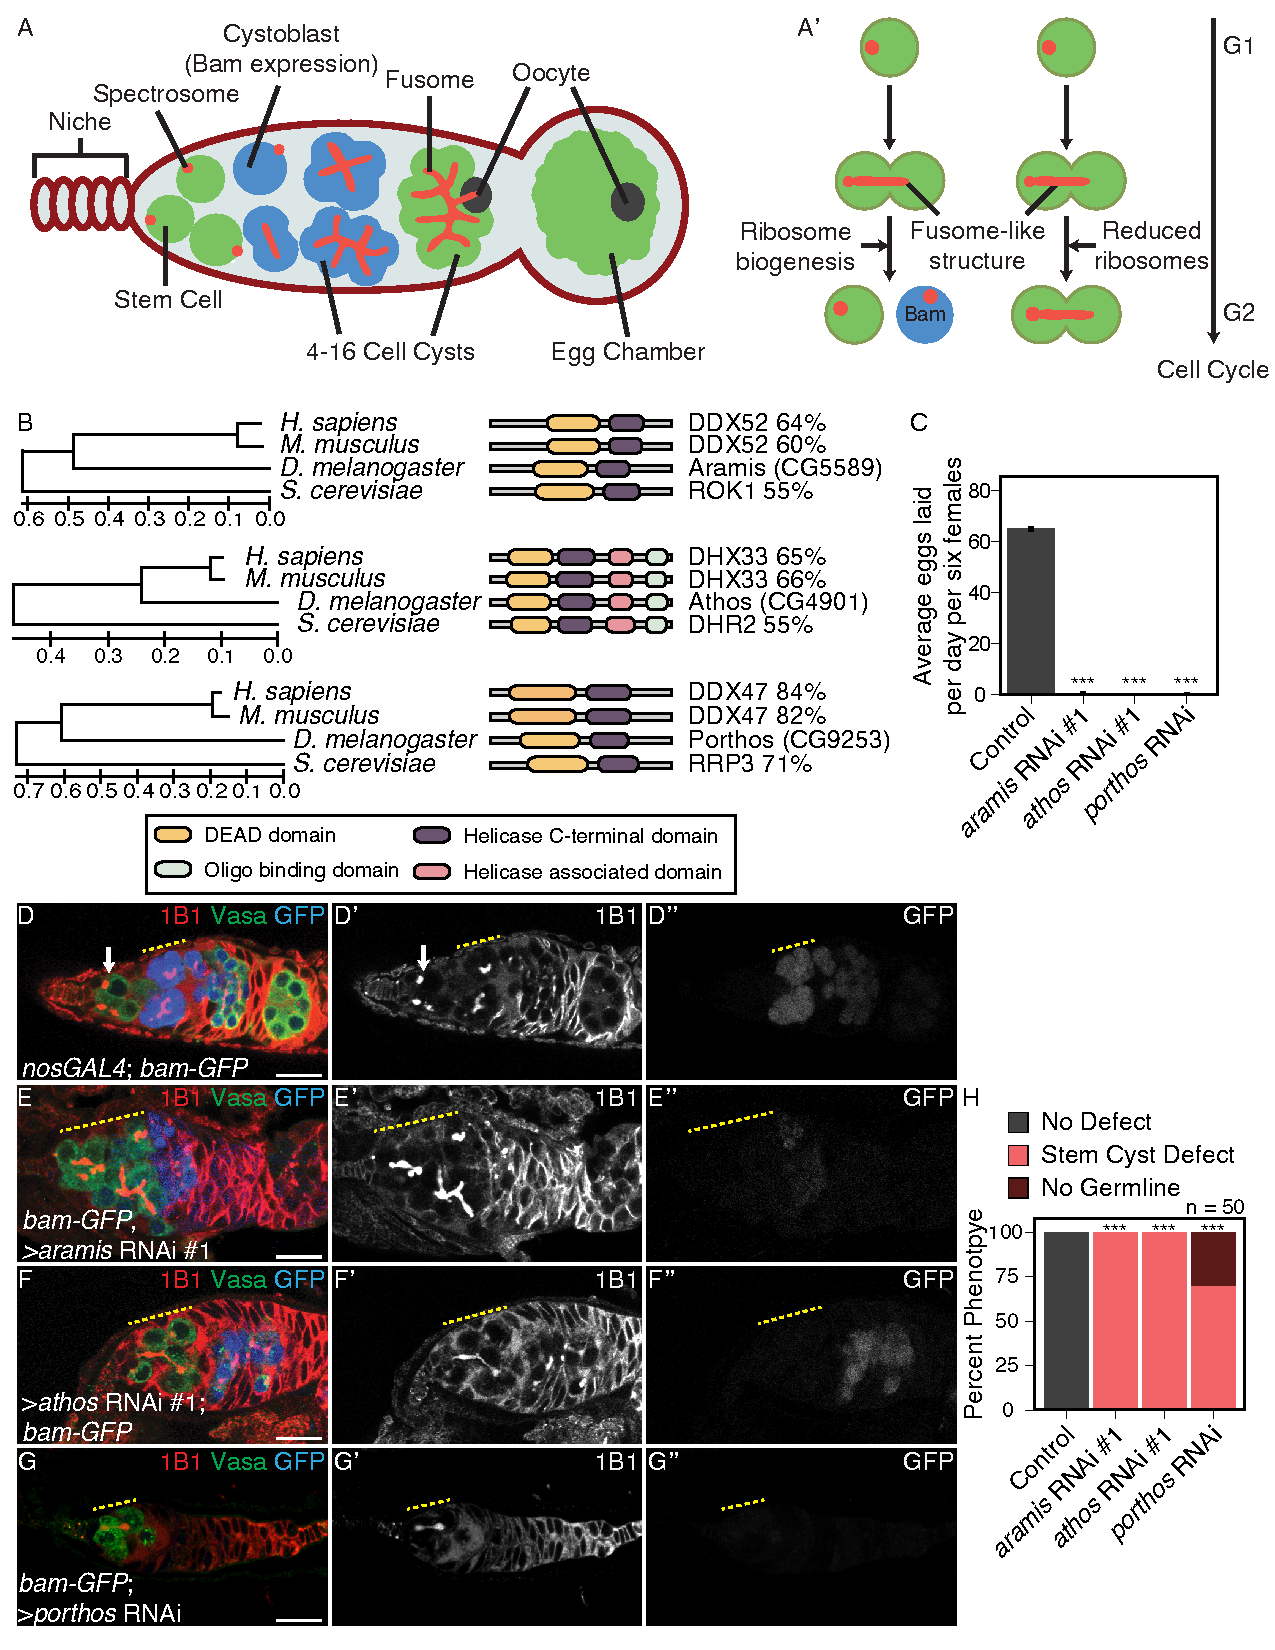
\includegraphics[width=0.98\linewidth]{./figure/Ribosome Biogenesis/Ribosome Biogenesis 1} \end{center}

\setstretch{1.0}

\setlength\parindent{0pt}(\textbf{A}) Schematic of \emph{Drosophila} germarium. Germline stem cells are attached to the somatic niche (dark red). The stem cells divide and give rise to a stem cell and a cystoblast (CB) that expresses the differentiation factor Bag-of-marbles (Bam). GSCs and CBs are marked by spectrosomes. The CB undergoes four incomplete mitotic divisions giving rise to a 16-cell cyst (blue). Cysts are marked by branched spectrosome structures known as fusomes (red). One cell of the 16-cell cyst is specified as the oocyte. The 16-cell cyst is encapsulated by the surrounding somatic cells giving rise to an egg chamber. (\textbf{A'}) Ribosome biogenesis promotes GSC cytokinesis and differentiation. Disruption of ribosome biogenesis results in undifferentiated stem cyst accumulation. (\textbf{B}) Conservation of \emph{aramis}, \emph{athos}, and \emph{porthos} between \emph{H. sapiens}, \emph{D. melanogaster}, and \emph{S. cerevisiae} (left), trees are drawn to scale, with branch lengths measured in the number of substitutions per site. Representation of conserved protein domains for three RNA helicases in \emph{Drosophila} compared to \emph{H. sapiens} and \emph{S. cerevisiae} orthologs (right). Percentage values represent similarity to \emph{Drosophila} orthologs. (\textbf{C}) Egg laying assay after germline RNAi knockdown of \emph{aramis}, \emph{athos} or \emph{porthos} indicating a loss of fertility compared to \emph{nosGAL4}, driver control (n=3 trials). *** = p \textless{} 0.001, Tukey's post-hoc test after one-way ANOVA, p \textless{} 0.001. Error bars represent standard error (SE). (\textbf{D-G''}) Confocal micrographs of ovaries from control, \emph{UAS-Dcr2; nosGAL4; bam-GFP} (\textbf{D-D''}) and germline RNAi depletion targeting (\textbf{E-E''}) \emph{aramis}, (\textbf{F-F''}) \emph{athos} or (\textbf{G-G''}) \emph{porthos} stained for 1B1 (red, left grayscale), Vasa (green), and Bam-GFP (blue, right grayscale). Depletion of these genes (\textbf{E-G''}) results in a characteristic phenotype in which early germ cells are connected marked by a 1B1 positive, fusome-like structure highlighted by a yellow dotted line in contrast to the single cells present in (\textbf{D-D''}) controls (white arrow) or differentiating cysts (yellow dashed line). Bam expression, if present, is followed by loss of the germline. (\textbf{H}) Phenotype quantification of ovaries depleted of \emph{aramis}, \emph{athos} or \emph{porthos} compared to control ovaries (n=50 ovarioles, df=2, *** = p \textless{} 0.001, Fisher's exact tests with Holm-Bonferroni correction). Scale bars are 15 micron.

\setstretch{2.0}

\hypertarget{to-determine-if-nuclear-setdb1-was-required-to-repress-rps19b-gfp-post-oocyte-specification-we-depleted-wde-in-the-germline-and-independently-assayed-for-setdb1-nuclear-localization-h3k9me3-and-rps19b-gfp-figure-s1c.-gkd-of-wde-resulted-in-loss-of-nuclear-setdb1-in-the-differentiated-stages-of-oogenesis-without-affecting-cytoplasmic-levels-in-the-undifferentiated-stages-figure-s1d-f.-whereas-gkd-of-setdb1-reduced-h3k9me3-throughout-oogenesis-gkd-of-wde-reduced-h3k9me3-only-in-the-differentiated-egg-chambers-but-not-in-the-undifferentiated-stages-figure-s1g-j.-we-found-that-gkd-of-wde-like-gkd-of-setdb1-results-in-ectopic-rps19b-gfp-protein-expression-in-the-egg-chambers-without-affecting-levels-in-the-undifferentiated-stages-figure-1c-g.-in-addition-to-upregulation-of-rps19b-gfp-gkd-of-both-setdb1-and-wde-resulted-in-egg-chambers-that-did-not-grow-in-size-and-died-mid-oogenesis-as-previously-reported-figure-s1k-cloughepigeneticregulationoogenesis2014kochwindeidrosophilahomolog2009.-thus-repression-of-the-rps19b-gfp-reporter-in-the-differentiated-egg-chambers-requires-nuclear-setdb1.}{%
\chapter{\texorpdfstring{To determine if nuclear SETDB1 was required to repress \emph{RpS19b-GFP} post-oocyte specification, we depleted \emph{wde} in the germline and independently assayed for SETDB1 nuclear localization, H3K9me3, and RpS19b-GFP (Figure S1C). GKD of \emph{wde} resulted in loss of nuclear SETDB1 in the differentiated stages of oogenesis without affecting cytoplasmic levels in the undifferentiated stages (Figure S1D-F). Whereas GKD of \emph{SETDB1} reduced H3K9me3 throughout oogenesis, GKD of \emph{wde} reduced H3K9me3 only in the differentiated egg chambers but not in the undifferentiated stages (Figure S1G-J). We found that GKD of \emph{wde}, like GKD of \emph{SETDB1}, results in ectopic RpS19b-GFP protein expression in the egg chambers without affecting levels in the undifferentiated stages (Figure 1C-G). In addition to upregulation of RpS19b-GFP, GKD of both \emph{SETDB1} and \emph{wde} resulted in egg chambers that did not grow in size and died mid-oogenesis as previously reported (Figure S1K) (Clough et al., 2014; Koch et al., 2009). Thus, repression of the \emph{RpS19b-GFP} reporter in the differentiated egg chambers requires nuclear SETDB1.}{To determine if nuclear SETDB1 was required to repress RpS19b-GFP post-oocyte specification, we depleted wde in the germline and independently assayed for SETDB1 nuclear localization, H3K9me3, and RpS19b-GFP (Figure S1C). GKD of wde resulted in loss of nuclear SETDB1 in the differentiated stages of oogenesis without affecting cytoplasmic levels in the undifferentiated stages (Figure S1D-F). Whereas GKD of SETDB1 reduced H3K9me3 throughout oogenesis, GKD of wde reduced H3K9me3 only in the differentiated egg chambers but not in the undifferentiated stages (Figure S1G-J). We found that GKD of wde, like GKD of SETDB1, results in ectopic RpS19b-GFP protein expression in the egg chambers without affecting levels in the undifferentiated stages (Figure 1C-G). In addition to upregulation of RpS19b-GFP, GKD of both SETDB1 and wde resulted in egg chambers that did not grow in size and died mid-oogenesis as previously reported (Figure S1K) (Clough et al., 2014; Koch et al., 2009). Thus, repression of the RpS19b-GFP reporter in the differentiated egg chambers requires nuclear SETDB1.}}\label{to-determine-if-nuclear-setdb1-was-required-to-repress-rps19b-gfp-post-oocyte-specification-we-depleted-wde-in-the-germline-and-independently-assayed-for-setdb1-nuclear-localization-h3k9me3-and-rps19b-gfp-figure-s1c.-gkd-of-wde-resulted-in-loss-of-nuclear-setdb1-in-the-differentiated-stages-of-oogenesis-without-affecting-cytoplasmic-levels-in-the-undifferentiated-stages-figure-s1d-f.-whereas-gkd-of-setdb1-reduced-h3k9me3-throughout-oogenesis-gkd-of-wde-reduced-h3k9me3-only-in-the-differentiated-egg-chambers-but-not-in-the-undifferentiated-stages-figure-s1g-j.-we-found-that-gkd-of-wde-like-gkd-of-setdb1-results-in-ectopic-rps19b-gfp-protein-expression-in-the-egg-chambers-without-affecting-levels-in-the-undifferentiated-stages-figure-1c-g.-in-addition-to-upregulation-of-rps19b-gfp-gkd-of-both-setdb1-and-wde-resulted-in-egg-chambers-that-did-not-grow-in-size-and-died-mid-oogenesis-as-previously-reported-figure-s1k-cloughepigeneticregulationoogenesis2014kochwindeidrosophilahomolog2009.-thus-repression-of-the-rps19b-gfp-reporter-in-the-differentiated-egg-chambers-requires-nuclear-setdb1.}}

SETDB1 and Wde repress genes that are primarily expressed prior to oocyte specification

To determine if SETDB1 and Wde repress other differentiation-promoting genes in addition to \emph{RpS19b}, we performed RNA Sequencing (RNA-seq). We compared ovaries from \emph{SETDB1-} and \emph{wde-} GKD flies to ovaries from wild-type (WT) flies, including young virgin flies which lack late-stage egg chambers. Principal component analysis of the RNA-seq data revealed that \emph{SETDB1} and \emph{wde} ovary~transcriptomes~closely resembles young virgin WT rather than adult WT (Figure S2A). Using a 1.5-fold cut off (\(Fold Change (FC) \ge |1.5|\)) and False Discovery Rate (FDR)\textless0.05, we found that compared to young virgin WT control, 2316 genes were upregulated and 1972 were downregulated in \emph{SETDB1} GKD ovaries, and 1075 genes were upregulated and 442 were downregulated in \emph{wde-}GKD ovaries (Figure 2A-B) (Supplemental Table 1). Moreover, comparing \emph{wde}- to \emph{SETDB1}- GKD ovaries showed significant overlap of the upregulated (80\%) and downregulated (75\%) transcripts, suggesting that \emph{SETDB1} and \emph{Wde} co-regulate a cohort of genes during oogenesis (Figure 2C; Figure S2B).

\hypertarget{setdb1-and-wde-are-known-to-repress-gene-expression-thus-we-first-focused-on-mrnas-with-increased-levels-in-the-gkd-ovaries-cloughepigeneticregulationoogenesis2014osumiessentialroleswindei2019.-gene-ontology-go-analysis-of-the-shared-upregulated-rnas-indicated-that-many-were-genes-involved-in-differentiation-figure-2d.-among-the-upregulated-rnas-was-rps19b-validating-our-initial-screen-as-well-as-genes-that-promote-synaptonemal-complex-formation-such-as-sunn-ord-and-cona-figure-2e-figure-s2c-e.-in-addition-the-blanks-mrna-which-is-highly-expressed-only-in-gscs-cystoblasts-and-early-cysts-of-wt-was-upregulated-and-ectopically-expressed-in-the-egg-chambers-of-setdb1--and-wde-gkd-ovaries-figure-2f-figure-s2f-i-blattrnadegradationrequired2021.-blanks-is-a-component-of-a-nuclear-sirna-pathway-that-has-critical-roles-in-the-testis-but-does-not-have-any-overt-function-during-oogenesis-gerbasiblanksnuclearsirna2011.-thus-setdb1-and-wde-repress-a-cohort-of-rnas-that-are-either-critical-for-transition-from-gsc-to-an-oocyte-or-merely-expressed-during-early-oogenesis.}{%
\chapter{\texorpdfstring{SETDB1 and Wde are known to repress gene expression, thus we first focused on mRNAs with increased levels in the GKD ovaries (Clough et al., 2014; Osumi et al., 2019). Gene Ontology (GO) analysis of the shared upregulated RNAs indicated that many were genes involved in differentiation (Figure 2D). Among the upregulated RNAs was \emph{RpS19b}, validating our initial screen, as well as genes that promote synaptonemal complex formation such as \emph{sunn, ord} and \emph{cona} (Figure 2E; Figure S2C-E). In addition, the \emph{blanks} mRNA, which is highly expressed only in GSCs, cystoblasts and early cysts of WT, was upregulated and ectopically expressed in the egg chambers of \emph{SETDB1-} and \emph{wde-}GKD ovaries (Figure 2F; Figure S2F-I) (Blatt et al., 2021). Blanks is a component of a nuclear siRNA pathway that has critical roles in the testis but does not have any overt function during oogenesis (Gerbasi et al., 2011). Thus, \emph{SETDB1} and \emph{wde} repress a cohort of RNAs that are either critical for transition from GSC to an oocyte or merely expressed during early oogenesis.}{SETDB1 and Wde are known to repress gene expression, thus we first focused on mRNAs with increased levels in the GKD ovaries (Clough et al., 2014; Osumi et al., 2019). Gene Ontology (GO) analysis of the shared upregulated RNAs indicated that many were genes involved in differentiation (Figure 2D). Among the upregulated RNAs was RpS19b, validating our initial screen, as well as genes that promote synaptonemal complex formation such as sunn, ord and cona (Figure 2E; Figure S2C-E). In addition, the blanks mRNA, which is highly expressed only in GSCs, cystoblasts and early cysts of WT, was upregulated and ectopically expressed in the egg chambers of SETDB1- and wde-GKD ovaries (Figure 2F; Figure S2F-I) (Blatt et al., 2021). Blanks is a component of a nuclear siRNA pathway that has critical roles in the testis but does not have any overt function during oogenesis (Gerbasi et al., 2011). Thus, SETDB1 and wde repress a cohort of RNAs that are either critical for transition from GSC to an oocyte or merely expressed during early oogenesis.}}\label{setdb1-and-wde-are-known-to-repress-gene-expression-thus-we-first-focused-on-mrnas-with-increased-levels-in-the-gkd-ovaries-cloughepigeneticregulationoogenesis2014osumiessentialroleswindei2019.-gene-ontology-go-analysis-of-the-shared-upregulated-rnas-indicated-that-many-were-genes-involved-in-differentiation-figure-2d.-among-the-upregulated-rnas-was-rps19b-validating-our-initial-screen-as-well-as-genes-that-promote-synaptonemal-complex-formation-such-as-sunn-ord-and-cona-figure-2e-figure-s2c-e.-in-addition-the-blanks-mrna-which-is-highly-expressed-only-in-gscs-cystoblasts-and-early-cysts-of-wt-was-upregulated-and-ectopically-expressed-in-the-egg-chambers-of-setdb1--and-wde-gkd-ovaries-figure-2f-figure-s2f-i-blattrnadegradationrequired2021.-blanks-is-a-component-of-a-nuclear-sirna-pathway-that-has-critical-roles-in-the-testis-but-does-not-have-any-overt-function-during-oogenesis-gerbasiblanksnuclearsirna2011.-thus-setdb1-and-wde-repress-a-cohort-of-rnas-that-are-either-critical-for-transition-from-gsc-to-an-oocyte-or-merely-expressed-during-early-oogenesis.}}

To determine when during oogenesis SETDB1 and Wde act to repress genes, we analyzed available RNA-seq libraries that were enriched for GSCs, cystoblasts, and cysts, early egg chambers and late-stage egg chambers (McCarthy, Sarkar, Martin, et al., 2019b). We found that \emph{SETDB1}/\emph{wde}-regulated RNAs decreased after the cyst stages and their levels were attenuated in the later stages of oogenesis compared to non-targets (Figure 2G, Figure S2J-L) (McCarthy, Sarkar, Martin, et al., 2019b). This reduction did not happen in absence of \emph{SETDB1} and \emph{wde} (Figure 2G). RNA \emph{in situ} analysis of \emph{blanks}, and \emph{RpS19b} revealed that these mRNAs are present in the early stages of oogenesis and are attenuated after oocyte specification in controls but that these RNAs persisted in \emph{SETDB1} and \emph{wde} GKD egg chambers (Figure 2H-O). Thus, mRNAs that are broadly expressed prior to oocyte specification, become repressed by SETDB1 and Wde in differentiated egg chambers.

SETDB1 represses transcription of a subset of targets by increasing H3K9me3 enrichment

To investigate whether SETDB1/Wde-regulated mRNAs are repressed at the level of transcription, we examined a subset of nascent mRNAs (pre-mRNAs) by qRT-PCR. Indeed, the levels of nascent \emph{RpS19b}, \emph{ord}, \emph{sunn}, \emph{cona} and \emph{blanks} mRNAs were increased in \emph{SETDB1}/\emph{wde-}GKDs ovaries compared to control WT ovaries (Figure S3A-B). These data suggest that transcription of these genes increases upon loss of SETDB1 or Wde.

To determine if the SETDB1-dependent repression of these genes involves changes in H3K9me3, we performed CUT\&RUN (Ahmad, 2018; Skene \& Henikoff, 2017) on adult WT ovaries enriched for differentiated egg chambers where these genes are repressed (Figure 2G). Analysis of CUT\& RUN data from adult WT showed enrichment of H3K9me3 marks on previously identified SETDB1 targets and genes containing heterochromatin such as PHD Finger Protein 7 (\emph{phf7)} and \emph{light} (\emph{lt)} respectively validating our CUT\&RUN data (Figure 3A-B; Figure S3C) (Devlin, Bingham, \& Wakimoto, 1990; Smolko et al., 2018). As genes in \emph{Drosophila} genome are closely packed, we only analyzed the gene body from 5'UTR to the end of the 3'UTR to unambiguously identify SETDB1 regulated genes (Schwartz \& Cavalli, 2017). We found that 1593 out of 2,316 genes upregulated upon loss of SETDB1 are enriched for H3K9me3 marks compared to IgG negative control (Figure 3C). In addition, we found that 888 genes lose H3K9me3 on their gene bodies upon GKD of \emph{SETDB1} including \emph{RpS19b} and ATP-dependent chromatin assembly factor (\emph{Acf)} (Figure 3D-F). The upregulated genes that do not show changes to H3K9me3 marks within the gene body may be regulated by elements outside of the gene body or indirectly. Importantly, taken together, our data suggest that SETDB1 is required for H3K9me3 enrichment and transcriptional repression of a cohort of early-oogenesis genes in the egg chamber.

\hypertarget{setdb1-is-required-for-transposon-repression-during-oogenesis-andersenheterochromatindependenttranscriptionmachinery2017ranganpirnaproductionrequires2011a-and-the-upregulation-of-transposons-can-affect-gene-expression-sienskitranscriptionalsilencingtransposons2012upadhyaytransposondysregulationmodulates2016.-however-we-found-that-the-upregulation-of-genes-in-the-differentiated-stages-that-we-observed-upon-depletion-of-setdb1-was-not-due-to-the-secondary-effect-of-transposon-upregulation-as-the-expression-of-rps19b-reporter-was-not-altered-in-germline-depleted-of-aubergine-aub-a-critical-component-of-the-pirna-pathway-figure-s3d-f-chencutoffauberginemutations2007czechpirnaguidedgenomedefense2018malonespecializedpirnapathways2009wangslicingbindingago32015.-nor-did-aub-depletion-cause-mid-oogenesis-death-as-we-observed-in-setdb1-and-wde-gkds-figure-s3d-f-chencutoffauberginemutations2007wilsonaubergineenhancesoskar1996.-overall-our-data-suggest-that-loss-of-setdb1-derepresses-a-subset-of-genes-during-late-oogenesis-via-decreased-h3k9me3-independent-of-transposon-dysregulation.}{%
\chapter{\texorpdfstring{\emph{SETDB1} is required for transposon repression during oogenesis (Andersen, Tirian, Vunjak, \& Brennecke, 2017; Rangan et al., 2011), and the upregulation of transposons can affect gene expression (Sienski, Dönertas, \& Brennecke, 2012; Upadhyay et al., 2016). However, we found that the upregulation of genes in the differentiated stages that we observed upon depletion of \emph{SETDB1} was not due to the secondary effect of transposon upregulation as the expression of \emph{RpS19b} reporter was not altered in germline depleted of \emph{aubergine} (\emph{aub}), a critical component of the piRNA pathway (Figure S3D-F) (Chen, Pane, \& Schüpbach, 2007; Czech et al., 2018; Malone et al., 2009; Wang et al., 2015). Nor, did \emph{aub} depletion cause mid-oogenesis death as we observed in \emph{SETDB1} and \emph{wde} GKDs (Figure S3D-F) (Chen et al., 2007; Wilson, Connell, \& Macdonald, 1996). Overall, our data suggest that loss of \emph{SETDB1} derepresses a subset of genes during late oogenesis via decreased H3K9me3, independent of transposon dysregulation.}{SETDB1 is required for transposon repression during oogenesis (Andersen, Tirian, Vunjak, \& Brennecke, 2017; Rangan et al., 2011), and the upregulation of transposons can affect gene expression (Sienski, Dönertas, \& Brennecke, 2012; Upadhyay et al., 2016). However, we found that the upregulation of genes in the differentiated stages that we observed upon depletion of SETDB1 was not due to the secondary effect of transposon upregulation as the expression of RpS19b reporter was not altered in germline depleted of aubergine (aub), a critical component of the piRNA pathway (Figure S3D-F) (Chen, Pane, \& Schüpbach, 2007; Czech et al., 2018; Malone et al., 2009; Wang et al., 2015). Nor, did aub depletion cause mid-oogenesis death as we observed in SETDB1 and wde GKDs (Figure S3D-F) (Chen et al., 2007; Wilson, Connell, \& Macdonald, 1996). Overall, our data suggest that loss of SETDB1 derepresses a subset of genes during late oogenesis via decreased H3K9me3, independent of transposon dysregulation.}}\label{setdb1-is-required-for-transposon-repression-during-oogenesis-andersenheterochromatindependenttranscriptionmachinery2017ranganpirnaproductionrequires2011a-and-the-upregulation-of-transposons-can-affect-gene-expression-sienskitranscriptionalsilencingtransposons2012upadhyaytransposondysregulationmodulates2016.-however-we-found-that-the-upregulation-of-genes-in-the-differentiated-stages-that-we-observed-upon-depletion-of-setdb1-was-not-due-to-the-secondary-effect-of-transposon-upregulation-as-the-expression-of-rps19b-reporter-was-not-altered-in-germline-depleted-of-aubergine-aub-a-critical-component-of-the-pirna-pathway-figure-s3d-f-chencutoffauberginemutations2007czechpirnaguidedgenomedefense2018malonespecializedpirnapathways2009wangslicingbindingago32015.-nor-did-aub-depletion-cause-mid-oogenesis-death-as-we-observed-in-setdb1-and-wde-gkds-figure-s3d-f-chencutoffauberginemutations2007wilsonaubergineenhancesoskar1996.-overall-our-data-suggest-that-loss-of-setdb1-derepresses-a-subset-of-genes-during-late-oogenesis-via-decreased-h3k9me3-independent-of-transposon-dysregulation.}}

\hypertarget{setdb1-is-required-for-the-expression-of-npc-components}{%
\chapter{SETDB1 is required for the expression of NPC components}\label{setdb1-is-required-for-the-expression-of-npc-components}}

GO term analysis of downregulated targets of \emph{SETDB1}/\emph{wde} GKD included
genes that regulate transposition, consistent with the previously
described role of SETDB1/Wde in the piRNA pathway and those that
regulate proper oocyte development, consistent with the previously
described phenotype (\textbf{Figure
4A})(Andersen et al., 2017; Clough et al., 2007; Koch et al., 2009; Rangan et al., 2011).

Unexpectedly, we observed that genes involved in nucleocytoplasmic
transport were downregulated in \emph{SETDB1/wde}-GKD ovaries as compared to
controls (\textbf{Figure 4A}). Nucleocytoplasmic transport is mediated by
Nucleopore complexes (NPCs), which span the nuclear membrane and consist
of a cytoplasmic ring, a central scaffold spanning the nuclear envelope,
and a nuclear ring and basket (\textbf{Figure 4B})
(M. Capelson et al., 2010a; Doucet \& Hetzer, 2010; Gozalo \& Capelson, 2016). Beyond regulating nucleocytoplasmic
transport, NPCs also regulate gene transcription, for instance by
anchoring and maintaining heterochromatic domains
(Capelson \& Hetzer, 2009; Hou \& Corces, 2010; Iglesias et al., 2020; Sarma \& Willis, n.d.; Sood \& Brickner, 2014).
We found that GKD of \emph{SETDB1}/\emph{wde} in the germline resulted in
downregulation of 18 out of \textasciitilde30 nucleoporins (Nups) that make up the
Nucleopore complex in \emph{Drosophila} (\textbf{Figure 4C}), including a germline
enriched \emph{Nup154} that is critical for oogenesis
(Colozza et al., 2011; Gigliotti et al., 1998; Grimaldi, Cozzolino, Malva, Graziani, \& Gigliotti, 2007). The Nups that were
downregulated upon depletion of \emph{SETDB1} and \emph{wde} were not isolated to
one specific NPC subcomplex (\textbf{Figure 4B-C}).

We found that nascent mRNAs corresponding to the \emph{SETDB1/Wde} targets
\emph{Nup154}, \emph{Nup205} and \emph{Nup107} were downregulated in \emph{SETDB1}/\emph{wde}-GKD
ovaries, whereas the non-target \emph{Nup62} was unaffected, suggesting that
SETDB1/Wde promotes transcription of a cohort of \emph{Nups} (\textbf{Figure
4D})\textbf{.} In addition, the levels of a Nup107-RFP fusion protein, under
endogenous control (Katsani, Karess, Dostatni, \& Doye, 2008), were
significantly reduced in the cysts and egg chambers of \emph{SETDB1-} and
\emph{wde-}GKD compared to controls (\textbf{Figure S4A-D}).

To determine if loss of \emph{Nup} expression in \emph{SETDB1}/\emph{wde-}GKD ovaries
resulted in loss of NPC formation, we performed immunofluorescence with
an antibody that is known to mark NPCs in \emph{Drosophila}
(Capelson et al., 2010b; Davis \& Blobel, 1987; Hampoelz et al., 2019; Kuhn, Pascual-Garcia, Gozalo, Little, \& Capelson, 2019). We found that NPC levels were
reduced in the egg chambers of \emph{SETDB1}/\emph{wde-}GKD ovaries compared to
controls (\textbf{Figure 4E-H}), but the nuclear lamina was unaffected
(\textbf{Figure S4E-H}), and NPCs in the soma were also unaffected (\textbf{Figure
4I}). Thus, \emph{SETDB1}/\emph{wde} are required for the proper expression of
Nups and NPC formation after oocyte specification.

Heterochromatic genes and piRNA clusters require heterochromatin to
promote their transcription (Rangan et al., 2011; Weiler \& Wakimoto, 1995). Although we found that
\emph{SETDB1} is required for upregulation of Nups, CUT\&RUN analysis of
H3K9me3 marks revealed that only 3 of the \emph{Nup} genes had any enrichment
of H3K9me3 (\emph{Mbo}, \emph{Nup188}, \emph{Gp210}). Moreover, among
\emph{SETDB1}-regulated \emph{Nups}, only Gp210 showed any heterochromatic
enrichment \textbf{(Supplemental Table 2).} Taken together, we find that
\emph{SETDB1} promotes proper expression of \emph{Nups} by a yet unknown mechanism
in the germline.

Nucleoporins are required to maintain heterochromatin domains at the nuclear periphery

Our data so far indicate that, in \emph{Drosophila} female germline,
heterochromatin formation mediated by SETDB1 is required for proper NPC
formation by promoting proper expression of a subset of \emph{Nups} including
\emph{Nup107} and \emph{Nup154} (\textbf{Figure 4C}). In yeast, a subset of Nups are
part of the heterochromatin proteome and are required to cluster and
maintain heterochromatin at the NPC
(Iglesias et al., 2020). This subset includes Nup107
and the yeast homolog of Nup154, Nup155, which both have reduced
expression in \emph{SETDB1/Wde}-GKD compared to controls. We hypothesized
that in \emph{Drosophila,} SETDB1 could promote silencing of early oogenesis
genes by promoting heterochromatin formation. This heterochromatin then
promotes expression of Nups and NPC formation, which can then help
maintain heterochromatin by anchoring it to nuclear periphery and thus
promoting silencing of early-oogenesis genes.

To first determine if heterochromatin and nucleoporins associate in
\emph{Drosophila} female germline, we utilized antibody against H3K9me3 to
mark heterochromatin and Nup107-RFP to mark NPCs in WT ovarioles
(Katsani et al., 2008; Rangan et al., 2011). We found that H3K9me3 domains
were often at the nuclear periphery, in close proximity with Nup107-RFP
(\textbf{Figure 5A-A2, E}). Next, to determine if loss of \emph{Nups} leads to
loss of heterochromatin, we first depleted \emph{Nup154} and probed for
heterochromatin formation. We chose \emph{Nup154}, as its loss of function
phenotype of \emph{Nup154} has been well described
(Gigliotti et al., 1998; Grimaldi et al., 2007). We found that GKD of
\emph{Nup154} in the germline, resulted in egg chambers that do not grow and
die mid-oogenesis as previously described for \emph{Nup154} mutants \textbf{(Figure
S5A-B2)} (Gigliotti et al., 1998). In addition, depletion
of \emph{Nup154} results in proper translocation of SETDB1 from the cytoplasm
to the nucleus suggesting that transport of SETDB1 into the nucleus is
not grossly affected \textbf{(Figure S5C-D1)}. By staining for H3K9me3 marks,
we found that upon GKD of \emph{Nup154}, heterochromatin domains initially
form (\textbf{Figure S5E-F2)}. However, in the egg chambers of \emph{Nup 154} GKD,
the colocalization between H3K9me3 domains and Nup107-RFP levels at the
nuclear periphery were significantly reduced prior to significant
reduction of heterochromatin levels \textbf{(Figure 5A-D1}\emph{,} \textbf{Figure
S5E-F3, I)}. GKD of \emph{Nup107} also resulted in egg chambers that do not
grow and loss of heterochromatin \textbf{(Figure S5E-I)}. Thus, \emph{Nups 154}
and \emph{107,} which are positively regulated by \emph{SETDB1}, are required for
H3K9me3 localization at the nuclear periphery for H3K9me3 maintenance in
the female germline.

Nups are required for silencing early-oogenesis genes

\hypertarget{based-on-our-findings-above-that-nups-are-required-to-maintain-h3k9me3-levels-and-localization-we-hypothesized-that-they-are-also-required-to-silence-the-early-oogenesis-rnas-in-differentiated-egg-chambers.-to-test-this-hypothesis-we-depleted-nup154-and-nup107-in-the-germline-of-a-fly-carrying-the-rps19b-gfp-reporter.-we-found-that-gkd-of-these-nucleoporins-resulted-in-upregulation-of-rps19b-gfp-phenocopying-gkd-of-setdb1wde-figure-6a-c-figure-s6a-b1-d.-moreover-germline-depletion-of-nup62-which-is-within-the-npc-but-not-regulated-by-setdb1-also-resulted-in-upregulation-of-rps19bgfp-and-egg-chambers-that-did-not-grow-figure-s6a-d.-this-suggests-that-activity-of-npc-components-and-not-just-the-nups-regulated-by-setdb1-are-required-for-silencing-rps19b-gfp-reporter.}{%
\chapter{\texorpdfstring{Based on our findings above that Nups are required to maintain H3K9me3 levels and localization, we hypothesized that they are also required to silence the early-oogenesis RNAs in differentiated egg chambers. To test this hypothesis, we depleted \emph{Nup154} and \emph{Nup107} in the germline of a fly carrying the \emph{RpS19b-GFP} reporter. We found that GKD of these nucleoporins resulted in upregulation of RpS19b-GFP phenocopying GKD of \emph{SETDB1/wde} (Figure 6A-C; Figure S6A-B1, D). Moreover, germline depletion of \emph{Nup62,} which is within the NPC but not regulated by SETDB1, also resulted in upregulation of \emph{RpS19bGFP} and egg chambers that did not grow (Figure S6A-D). This suggests that activity of NPC components and not just the Nups regulated by SETDB1 are required for silencing \emph{RpS19b-GFP} reporter.}{Based on our findings above that Nups are required to maintain H3K9me3 levels and localization, we hypothesized that they are also required to silence the early-oogenesis RNAs in differentiated egg chambers. To test this hypothesis, we depleted Nup154 and Nup107 in the germline of a fly carrying the RpS19b-GFP reporter. We found that GKD of these nucleoporins resulted in upregulation of RpS19b-GFP phenocopying GKD of SETDB1/wde (Figure 6A-C; Figure S6A-B1, D). Moreover, germline depletion of Nup62, which is within the NPC but not regulated by SETDB1, also resulted in upregulation of RpS19bGFP and egg chambers that did not grow (Figure S6A-D). This suggests that activity of NPC components and not just the Nups regulated by SETDB1 are required for silencing RpS19b-GFP reporter.}}\label{based-on-our-findings-above-that-nups-are-required-to-maintain-h3k9me3-levels-and-localization-we-hypothesized-that-they-are-also-required-to-silence-the-early-oogenesis-rnas-in-differentiated-egg-chambers.-to-test-this-hypothesis-we-depleted-nup154-and-nup107-in-the-germline-of-a-fly-carrying-the-rps19b-gfp-reporter.-we-found-that-gkd-of-these-nucleoporins-resulted-in-upregulation-of-rps19b-gfp-phenocopying-gkd-of-setdb1wde-figure-6a-c-figure-s6a-b1-d.-moreover-germline-depletion-of-nup62-which-is-within-the-npc-but-not-regulated-by-setdb1-also-resulted-in-upregulation-of-rps19bgfp-and-egg-chambers-that-did-not-grow-figure-s6a-d.-this-suggests-that-activity-of-npc-components-and-not-just-the-nups-regulated-by-setdb1-are-required-for-silencing-rps19b-gfp-reporter.}}

\hypertarget{to-determine-if-nups-are-required-for-silencing-other-early-oogenesis-rnas-we-performed-rna-seq-and-compared-nup154-gkd-ovaries-with-young-ovaries-as-a-developmental-control-figure-s2a.-using-a-1.5-fold-cut-off-fold-change-fcge1.5-and-false-discovery-rate-fdr0.05-we-found-that-compared-to-control-in-nup154-gkd-2809-genes-are-upregulated-and-2922-genes-are-downregulated-figure-6d-supplemental-table-1.-strikingly-97-of-upregulated-genes-and-89-of-downregulated-setdb1wde-targets-overlapped-with-nup154-gkd-figure-6e-s6e.-nup154-was-involved-in-silencing-genes-that-promote-oocyte-differentiation-including-synaptonemal-complex-components-ord-sunn-and-cona-as-well-as-rps19b-figure-6f-s6f-h.-in-addition-gkd-of-nup154-also-resulted-in-upregulation-of-blanks-figure-6g.-the-levels-of-nup154-regulated-rnas-decreased-after-the-cyst-stage-when-the-oocyte-is-specified-in-contrast-to-non-targets-which-have-similar-rna-levels-at-all-stages-figure-6h-s6i-j.-thus-nup154-is-critical-for-silencing-early-oogenic-mrnas-in-the-differentiated-egg-chambers.}{%
\chapter{\texorpdfstring{To determine if Nups are required for silencing other early oogenesis RNAs, we performed RNA-seq, and compared \emph{Nup154} GKD ovaries with young ovaries as a developmental control (Figure S2A). Using a 1.5-fold cut off (\(Fold Change (FC)\ge|1.5|\)) and False discovery rate (FDR)\textless0.05), we found that compared to control, in \emph{Nup154} GKD 2809 genes are upregulated, and 2922 genes are downregulated (Figure 6D) (Supplemental Table 1). Strikingly, 97\% of upregulated genes and 89\% of downregulated \emph{SETDB1}/\emph{Wde} targets overlapped with \emph{Nup154} GKD (Figure 6E; S6E). \emph{Nup154} was involved in silencing genes that promote oocyte differentiation including synaptonemal complex components \emph{ord}, \emph{sunn} and \emph{cona} as well as \emph{RpS19b} (Figure 6F; S6F-H). In addition, GKD of \emph{Nup154} also resulted in upregulation of \emph{blanks} (Figure 6G). The levels of \emph{Nup154}-regulated RNAs decreased after the cyst stage, when the oocyte is specified, in contrast to non-targets, which have similar RNA levels at all stages (Figure 6H; S6I-J). Thus, Nup154 is critical for silencing early-oogenic mRNAs in the differentiated egg chambers.}{To determine if Nups are required for silencing other early oogenesis RNAs, we performed RNA-seq, and compared Nup154 GKD ovaries with young ovaries as a developmental control (Figure S2A). Using a 1.5-fold cut off (Fold Change (FC)\textbackslash ge\textbar1.5\textbar) and False discovery rate (FDR)\textless0.05), we found that compared to control, in Nup154 GKD 2809 genes are upregulated, and 2922 genes are downregulated (Figure 6D) (Supplemental Table 1). Strikingly, 97\% of upregulated genes and 89\% of downregulated SETDB1/Wde targets overlapped with Nup154 GKD (Figure 6E; S6E). Nup154 was involved in silencing genes that promote oocyte differentiation including synaptonemal complex components ord, sunn and cona as well as RpS19b (Figure 6F; S6F-H). In addition, GKD of Nup154 also resulted in upregulation of blanks (Figure 6G). The levels of Nup154-regulated RNAs decreased after the cyst stage, when the oocyte is specified, in contrast to non-targets, which have similar RNA levels at all stages (Figure 6H; S6I-J). Thus, Nup154 is critical for silencing early-oogenic mRNAs in the differentiated egg chambers.}}\label{to-determine-if-nups-are-required-for-silencing-other-early-oogenesis-rnas-we-performed-rna-seq-and-compared-nup154-gkd-ovaries-with-young-ovaries-as-a-developmental-control-figure-s2a.-using-a-1.5-fold-cut-off-fold-change-fcge1.5-and-false-discovery-rate-fdr0.05-we-found-that-compared-to-control-in-nup154-gkd-2809-genes-are-upregulated-and-2922-genes-are-downregulated-figure-6d-supplemental-table-1.-strikingly-97-of-upregulated-genes-and-89-of-downregulated-setdb1wde-targets-overlapped-with-nup154-gkd-figure-6e-s6e.-nup154-was-involved-in-silencing-genes-that-promote-oocyte-differentiation-including-synaptonemal-complex-components-ord-sunn-and-cona-as-well-as-rps19b-figure-6f-s6f-h.-in-addition-gkd-of-nup154-also-resulted-in-upregulation-of-blanks-figure-6g.-the-levels-of-nup154-regulated-rnas-decreased-after-the-cyst-stage-when-the-oocyte-is-specified-in-contrast-to-non-targets-which-have-similar-rna-levels-at-all-stages-figure-6h-s6i-j.-thus-nup154-is-critical-for-silencing-early-oogenic-mrnas-in-the-differentiated-egg-chambers.}}

To determine if \emph{Nup154} is required for H3K9me3 marks at SETDB1-regulated gene, loci such as \emph{RpS19b}, we carried out CUT\& RUN for H3K9me3 in control and \emph{Nup154} GKD. We found that 564 out of 622 genes displaying a loss in H3K9me3 in Nup154 GKD also show the same loss in \emph{SETDB1} GKD including \emph{RpS19b} and \emph{Acf} (Figure 6I; S6K-L) (Supplemental Table 2). Taken together, we find that Nups are required for silencing and H3K9me3 at a subset of \emph{SETDB1/Wde-}regulated loci.

\textbf{Silencing genes expressed during the early oogenesis stages is
required for maintaining oocyte fate}

We next asked why loss of \emph{SETDB1, wde} and \emph{Nups} results in egg
chambers that do not grow and die mid-oogenesis. Egg chambers with
oocyte specification or maintenance defects result in death of egg
chambers mid-oogenesis (Blatt et al., 2021). To
determine if there are oocyte specification or maintenance defects, we
stained GKD of \emph{SETDB1, wde} and \emph{Nup154} for the oocyte marker
Egalitarian (Egl) as well as Vasa and 1B1
(Mach \& Lehmann, 1997; Navarro et al., 2004). In the early stages of
oogenesis, as in control, GKD of \emph{SETDB1, wde} and \emph{Nup154} resulted in
one Egl positive cell, suggesting that oocyte is specified (\textbf{Figure
7A-E}). While initial Egl localization to oocytes appeared to be
normal, we cannot rule out subtle specification defects.

However, in the later egg chambers, compared to control ovariole, GKD of
\emph{SETDB1, wde} and \emph{Nup154} resulted in either mis-localization or
diffuse Egl expression suggesting loss of oocyte fate (\textbf{Figure 7A-E}).
Taken together, these data suggest that SETDB1, Wde and Nup154 are
required for maintaining the oocyte fate.

\textbf{Discussion}

Many maternally contributed mRNAs in oocytes are critical for early
development after fertilization (Calvi, Lilly, \& Spradling, 1998; Huynh \& St Johnston, 2004; Kugler \& Lasko, n.d.; Navarro et al., 2004; Telfer, 1975). We previously showed
that many mRNAs expressed in germ cells and the undifferentiated stages
of oogenesis must be selectively degraded and thus excluded from the
maternal contribution (Blatt et al., 2021). However,
the potential role of transcriptional silencing of germ cell and
GSC-enriched genes during oogenesis was unclear. Here, we found that
regulated translocation of SETDB1 into the nucleus during oocyte
specification is required to silence germ cell- and early
oogenesis-genes in the differentiated egg chambers (\textbf{Figure 7F}), and
that this process is essential to maintain oocyte fate. Thus, some genes
that are expressed in germ cells and some that promote differentiation
are transcriptionally silenced at the onset of oocyte specification
mediated by a feedback loop between heterochromatin and NPC.

\textbf{Regulated heterochromatin formation during oocyte specification
promotes germ cell to oocyte transition}

A large fraction of SETDB1 is cytoplasmic in the undifferentiated stages
of the germline. As the oocyte is being specified during
differentiation, SETDB1 becomes mostly nuclear
(Clough et al., 2014). This translocation of
SETDB1 to the nucleus during oocyte specification is mediated by Windei
(Wde), the \emph{Drosophila} ortholog of mAM/MCAF1
(Koch et al., 2009; Osumi et al., 2019).
Here we find that translocation of SETDB1 to the nucleus during oocyte
specification is required to silence germ cell and early-oogenesis genes
at the onset of oocyte specification. MCAF1 also regulates the
accumulation of SETDB1 in the nucleus in mammalian cells
(Tsusaka, Shimura, \& Shinkai, 2019). In addition, loss of \emph{SETDB1}
during mammalian oogenesis results in meiotic defects and infertility
(Eymery, Liu, Ozonov, Stadler, \& Peters, 2016). These data suggest
that regulated heterochromatin formation is conserved to promote proper
oogenesis in mammals.

We discovered that SETDB1 is required to silence two major classes of
genes. The first group is involved in GSC differentiation into an
oocyte, including critical genes that promote meiosis I. The second
group of genes are those that are merely expressed in the germ cells
prior to differentiation into an oocyte, but have no specific function
in the female germline such as \emph{blanks}
(Blatt et al., 2021; Gerbasi et al., 2011).
We propose that these genes that are silenced upon oocyte specification
are either detrimental to late oogenesis or early embryogenesis. Indeed,
it has been shown that overexpression of one such gene \emph{actin 57B}
(\emph{act57B),} which is repressed by SETDB1/Wde \textbf{(Supplemental Table 1)},
is detrimental to oogenesis (Blatt et al., 2021; Duan, Green, Tootle, \& Geyer, 2020). Remarkably, some of the mRNAs
encoded by genes that are transcriptionally silenced by SETDB1 during
this transition are also targeted at the post-transcriptional level for
degradation by members of the no go decay pathway such as \emph{blanks} and
\emph{Act57B} (Blatt et al., 2021). Thus, our data suggests
that the regulation of gene expression during the germ cell to oocyte
transition reflects a two-step process: transcriptional silencing
dependent on SETDB1, and post-transcriptional degradation of mRNAs to
exclude a cohort of germ cell mRNAs from the maternal contribution
(Blatt et al., 2021).

SETDB1 is guided to its target transposons and piRNA clusters mediated
by piRNAs
(Andersen et al., 2017; Czech et al., 2018; Koch et al., 2009; Osumi et al., 2019). However, our data suggests that the
piRNA pathway does not play a part in silencing germ cell and early
oogenesis RNAs. We find that loss of \emph{aub} does not result in
upregulation of \emph{RpS19b}. This result is consistent with the fact that
loss of \emph{aub} and \emph{piwi} in the germline does not result in egg chambers
that do not grow (Chen et al., 2007; Wilson et al., 1996). In somatic cells of the gonad,
loss of \emph{wde} function eliminates nuclear SETDB1 signal
(Osumi et al., 2019; Timms, Tchasovnikarova, Antrobus, Dougan, \& Lehner, 2016). However, upon depletion
of Wde, SETDB1 was still ubiquitinated, a requirement for its nuclear
retention (Osumi et al., 2019). This suggests that in
absence of Wde, SETDB1 can translocate to the nucleus but cannot find
its targets. Osumi \emph{et al.} (Osumi et al., 2019)
suggested that Wde could mediate SETDB1 recruitment to the its targets,
leading to H3K9me3 deposition. In mammals, it has been shown that
transcriptional factors such as the KRAB domain-containing Zinc finger
proteins recruit SETDB1 to the target genes for silencing, but such
transcription factors have not been identified in the female gonad
(Frietze, O'Geen, Blahnik, Jin, \& Farnham, 2010; Schultz, Ayyanathan, Negorev, Maul, \& Rauscher, 2002). Thus, SETDB1 targets germ cell
and early oogenesis genes for silencing independent of the piRNA pathway
but through a yet undetermined mechanism, either through Wde or through
yet undetermined transcription factors.

\textbf{Nucleopore complex and heterochromatin are in a feedback loop to
promote gene silencing}

The NPC not only mediates selective nucleo-cytoplasmic transport of
macromolecules but also regulates gene expression by anchoring chromatin
domains, including heterochromatin to the nuclear periphery
(Capelson et al., 2010a, 2010b; Holla et al., 2020; Iglesias et al., 2020; Sarma \& Willis, n.d.). In addition, in yeast, several
Nups are also part of the heterochromatin proteome suggesting that NPCs
can regulate gene expression by regulating heterochromatin
(Brickner et al., 2019; Iglesias et al., 2020). Consistent with these
observations, we find that in the female germline of \emph{Drosophila}, NPC
and heterochromatin are closely associated. Loss of NPCs due to
depletion of individual Nups results in loss of heterochromatin and
subsequent upregulation of germ cell and early oogenesis genes resulting
in oogenesis defects. The 97\% overlap of target genes between \emph{SETDB1},
\emph{wde} and \emph{Nup154} is indicative that Nups are functioning in the same
pathway as SETDB1. This suggests that in the female germline, not only
do NPCs associate with heterochromatin, but that NPCs also play a role
in maintaining heterochromatin and gene repression during germ cell to
oocyte transition.

Silencing of early oogenesis genes at the onset of oocyte specification
is timed with exit from mitotic cell cycle. \emph{Drosophila} nucleopore
complex consists of \textasciitilde30 different nucleoporins some of which are
solubilized during early mitotic cell division
(Güttinger, Laurell, \& Kutay, 2009; Laurell \& Kutay, 2011). Nucleoporins are recruited to
the chromatin in early anaphase followed by sequential reassembly of the
complex (Kiseleva, Rutherford, Cotter, Allen, \& Goldberg, 2001; Kutay, Jühlen, \& Antonin, 2021). During \emph{Drosophila}
oogenesis, in the premeiotic stage, the GSC divides to eventually
produce a 16-cell cyst (Huynh \& St Johnston, 2004; Koch et al., 1967; Lehmann, 2012; Spradling et al., 2011).
Prophase-I of meiosis begins in cysts where the oocyte is also specified
(Ables, 2015; Orr-Weaver, 1995). We find that nucleoporins
promote silencing of genes that are required for initiation of meiosis I
such as \emph{Rbfox1} and synaptonemal complex components \emph{ord}, \emph{sunn} and
\emph{cona} once the cysts have stopped dividing and the oocyte is being
specified. Taken together, our data suggests a mechanism wherein after
the mitotic division of cysts have ceased and meiosis I is initiated,
the reassembly of NPC simultaneously promotes silencing of the genes
required for the transition from mitotic GSC division to meiotic oocyte
specification.

While NPC association with heterochromatin has been described,
remarkably we find that loss of heterochromatin results in attenuated
expression of some but not all Nup mRNAs. Heterochromatic genes and
piRNA clusters require heterochromatin to promote their transcription
(Andersen et al., 2017; Devlin et al., 1990; Rangan et al., 2011). However, by analyzing CUT \&RUN
data and previously published ChIP data of H3K9me3 marks, we found that
only one Nup regulated by SETDB1 is enriched for H3K9me3 marks.
Therefore, SETDB1 indirectly promotes expression of Nups.

The number of genes that need to be silenced varies based on cell types
and developmental trajectory. How levels of heterochromatin are coupled
to their NPC docking sites in the cell was not known. Like
heterochromatin levels, the number of NPCs also varies by cell type and
during differentiation (McCloskey, Ibarra, \& Hetzer, 2018). How NPC
number is regulated during development was not fully understood. Our
findings in the female germline suggest an elegant tuning mechanism for
heterochromatin and its NPC docking sites. Heterochromatin promotes
levels of NPC which then promote heterochromatin maintenance by
tethering it to the nuclear periphery. We find that this loop can be
developmentally regulated by controlling levels of SETDB1 in the nucleus
mediated by conserved protein Wde to promote heterochromatin formation.

\textbf{Acknowledgements:}

We are grateful to all members of the Rangan laboratory for discussion
and comments on the manuscript. We also thank Dr.~Thomas Hurd and Dr.
Miler Lee for their comments on the manuscript. We would like to thank
Sontheimer lab for Blanks antibody, Lehmann lab for Egl antibody,
Bloomington Drosophila Stock Center, Vienna Drosophila Resource Center,
Transgenic GKD Project (NIH/NIGMS R01-GM084947), The BDGP Gene
Disruption Project, and FlyBase for fly stocks and reagents.
Furthermore, we would like to thank CFG Facility at the University at
Albany (UAlbany) for performing RNA-seq analyses. P.R. is funded by
NIH/NIGMS~(RO1GM11177 and RO1GM135628). M.A.S is funded by NIH NIGMS R35
138120 and A.V. is funded by R01DE030927.

\textbf{Materials and Methods}

\textbf{Fly lines}

The following RNAi stocks were used in this study; if more than one line
is listed, then both were quantitated and the first was shown in the
main figure: \emph{SETDB1} RNAi (Perrimon lab,
(Rangan et al., 2011), \emph{Wde} RNAi (Bloomington
\#33339), \emph{Nup154} RNAi (Bloomington \#34710), \emph{Nup62} RNAi (Bloomington
\#35695), \emph{Nup107} RNAi (Bloomington \#43189), \emph{Nup205} RNAi (VDRC
\#V38608).

The following tagged lines were used in this study: \emph{dSETDB1-HA}
(Bontron Lab) (Seum et al., 2007), \emph{RpS19b-GFP}
(Buszczak Lab, (McCarthy, Sarkar, Martin, et al., 2019b),
mRFP-Nup107 (Bloomington \#35516).

The following tissue-specific drivers and double balancer lines were
used in this study:~\emph{UAS-Dcr2;nosGAL4}~(Bloomington
\#25751),~\emph{nosGAL4;MKRS}/TM6 (Bloomington \#4442), and
\emph{If}/CyO\emph{;nosGAL4} (Lehmann Lab).

\textbf{Reagents for fly husbandry}

Flies were grown at 25-29°C and dissected between 0-3 days
post-eclosion.

Fly food was made using the procedures as previously described
(summer/winter mix) and narrow vials (Fisherbrand Drosophila Vials;
Fischer Scientific) were filled to approximately 10-12mL
(Flora et al., 2018).

\textbf{Dissection and Immunostaining}

Ovaries were dissected and teased apart with mounting needles in cold
PBS and kept on ice. All incubation was done with nutation. Samples were
fixed for 10 minutes in 5\% methanol-free formaldehyde. Ovaries were
washed in 0.5 mL PBT (1X PBS, 0.5\% Triton X-100, 0.3\% BSA) 4 times for 5
minutes each. Primary antibodies in PBT were added and incubated at 4°C
nutating overnight. Samples were next washed 3 times for 5 minutes each
in 0.5 mL PBT, and once in 0.5 mL PBT with 2\% donkey serum (Sigma) for
15 minutes. Secondary antibodies were added in PBT with 4\% donkey serum
and incubated at room temperature for 3-4 hours. Samples were washed 3
times for 10 minutes each in 0.5 mL of 1X PBST (0.2\% Tween 20 in 1x PBS)
and incubated in Vectashield with DAPI (Vector Laboratories) for 1 hour
before mounting.

The following primary antibodies were used: mouse anti-1B1 (1:20; DSHB),
Rabbit anti-Vasa (1:1,000; Rangan Lab), Chicken anti-Vasa (1:1,000;
Rangan Lab) (Upadhyay et al., 2016), Rabbit anti-GFP (1:2,000; abcam,
ab6556), Rabbit anti-H3K9me3 (1:500; Active Motif, AB\_2532132), Mouse
anti-H3K27me3 (1:500; abcam, ab6002), Rabbit anti-Egl (1:1,000; Lehmann
Lab), Mouse anti-NPC (1:2000; BioLegend, AB\_2565026) and Rat anti-HA
(1:500; Roche, 11 867 423 001). The following secondary antibodies were
used: Alexa 488 (Molecular Probes), Cy3 and Cy5 (Jackson Labs) were used
at a dilution of 1:500.

\textbf{Fluorescence Imaging}

The tissues were visualized, and images were acquired using a Zeiss
LSM-710 confocal microscope under 20X, 40X and 63X oil objective with
pinhole set to 1 airy unit. All gain, laser power, and other relevant
settings were kept constant for any immunostainings being compared.
Image processing was done using Fiji and gain adjustment and cropping
was performed in Photoshop CC 2019.

\textbf{Colocalization analysis}

Confocal images of control and Nup154-RNAi mutants labeled for
RFP-Nup107, H3K9me3, and DAPI were imported into Bitplane Imaris 9.6.2
for 3D reconstruction and colocalization analysis. Colocalization
between RFP-Nup107 and H3K9me3 was calculated on a per egg chamber basis
using the Surface-surface coloc function of Imaris and an automatic
threshold detection and the surface-to-surface coloc function. The
number of colocalized voxels was then normalized to the number of
H3K9me3 voxels (Valm et al., 2017).

\textbf{Egg laying assays}

Assays were conducted in vials with 3 control or experimental females
under testing and 1 wild type control males. Crosses were set up in
triplicate for both control and experimental. All flies were 1-day old
post-eclosion upon setting up the experiment. Cages were maintained at
29°C and plates were changed daily for counting. Analyses were performed
for 5 consecutive days. Number of eggs laid were counted and averaged.
Adult flies eclosed were counted from all the vials and averaged.

\textbf{RNA isolation}

Ovaries from flies were dissected in cold 1x PBS. RNA was isolated using
TRIzol (Invitrogen, 15596026) (Blatt et al., 2021; McCarthy, Sarkar, Martin, et al., 2019b).

RNA was treated with DNase (TURBO DNA-free Kit, Life Technologies,
AM1907), and then run on a 1\% agarose gel to check integrity of the RNA.

\textbf{RNA-seq library preparation and analysis}

Libraries were prepared using the Biooscientific kit. To generate mRNA
enriched libraries, total RNA was treated with poly(A)tail selection
beads (Bioo Scientific Corp., NOVA-512991). Manufacturer's instructions
of the NEXTflex Rapid Directional RNA-seq Kit (Bioo Scientific Corp.,
NOVA-5138-08) were followed, but RNA was fragmented for 13 minutes.
Library quality was assessed with a Fragment Analyzer (5200 Fragment
Analyzer System, AATI, Ankeny, IA, USA) following manufacturer's
instructions. Single-end mRNA sequencing (75 base pair reads) was
performed on biological duplicates from each genotype on an Illumina
NextSeq500 by the Center for Functional Genomics (CFG).

After quality assessment, the sequenced reads were aligned to the
\emph{Drosophila melanogaster} genome (UCSCdm6) using HISAT2 (version 2.1.0)
with the RefSeq-annotated transcripts as a guide (Kim et al., 2015).
Differential gene expression was assayed by DeSeq2, using a false
discovery rate (FDR) of 0.05, and genes with 2-fold or higher were
considered significant. The raw and unprocessed data for RNA-seq
generated during this study are available at Gene Expression Omnibus
(GEO) databank under accession number: GSE186982 (Token number:
wlenykcoldmzfqf). GO term enrichment on differentially expressed genes
was performed using Panther (Thomas et al., 2006).

\textbf{Fluorescent \emph{in situ} hybridization}

A modified \emph{in situ} hybridization procedure for \emph{Drosophila} ovaries
was followed. Probes were designed and generated by LGC Biosearch
Technologies using Stellaris® RNA FISH Probe Designer, with specificity
to target base pairs of target mRNAs. Ovaries (3 pairs per sample) were
dissected in RNase free 1X PBS and fixed in 1 mL of 5\% formaldehyde for
10 minutes. The samples were then permeabilized in 1mL of
Permeabilization Solution (PBST+1\% Triton-X) rotating in RT for 1 hour.
Samples were then washed in wash buffer for 5 minutes (10\% deionized
formamide and 10\% 20x SSC in RNase-free water). Ovaries were covered and
incubated overnight with 1ul of probe in hybridization solution (10\%
dextran sulfate, 1 mg/ml yeast tRNA, 2 mM RNaseOUT, 0.02 mg/ml BSA, 5x
SSC, 10\% deionized formamide, and RNase-free water) at 30°C. Samples
were then washed 2 times in 1 mL wash buffer for 30 minutes and mounted
in Vectashield.

\textbf{CUT\&RUN assay}

Ovaries from flies were dissected in ice cold 1x PBS and ovarioles were
separated by teasing after dissection with mounting needles. PBS was
removed and the samples were permeabilized in 1mL of Permeabilization
Solution (PBST+1\% Triton-X) rotating in RT for 1 hour. Samples were then
incubated overnight at 4°C in primary antibody dilutions in freshly
prepared BBT+ buffer (PBST + 1\% BSA + 0.5 mM Spermidine + 2 mM EDTA + 1
large Roche complete EDTA-free tablets). Primary antibody was replaced
with BBT+ buffer and quickly washed twice. Samples were then incubated
in \textasciitilde700 ng/ml of pAG-MNase in BBT+ buffer rotating for 4 hours at 25°C.
Samples were then quickly washed twice in wash+ buffer (20 mM HEPES
pH7.5 + 150 mM NaCl + 0.1\% BSA + 0.5 mM Spermidine + 1 large Roche
complete EDTA-free tablets in water). Samples were resuspended in 150 µl
Wash+C (wash+ + 100 mM CaCl\textsubscript{2}) and incubated for 45 minutes on nutator
at 4°C. The cleavage reaction was terminated by addition of 150 µl StopR
(NaCl final 200 mM + EDTA final 20 mM + 100µg/mL RNaseA) and incubating
the sample at 37°C for 30 minutes. Samples were then centrifuged at
16,000 x g for 5 minutes and 300 µl of the supernatant was collected for
DNA discovery. To the supernatant, 2 µL 10\% SDS and 2.5 µL of 20 mg /mL
Proteinase K was added and incubated at 50°C for 2 hours. Half of this
was kept as a backup and half was used in bead cleanup. 20 µL AmpureXP
bead slurry and 280 µL MXP buffer (20\% PEG8000 + 2.5 M NaCl + 10 mM
MgCl2 in water) was added to the sample and mixed thoroughly followed by
15 minutes incubation at RT. The beads were separated by magnet and
supernatant was discarded. The beads were carefully washed with 80\%
ethanol for 30 seconds, while on the magnetic stand and air dried for 2
minutes. The beads were then resuspended in 10 µL DNase free water.

\textbf{DNA seq library preparation and analysis}

The samples from CUT\&RUN assay were used for library preparation using
NEBNext® Ultra™ DNA Library Prep Kit for Illumina® (E7645, E7103) and
adaptor ligated DNA were prepared without size selection.

\textbf{CUT\&Run Data Analysis}

Cut\&Run libraries were sequenced as paired-end 75bp reads on the
Illumina NextSeq 500 at the University at Albany Center for Functional
Genomics. FASTQ files were aligned to the dm6 reference genome using
HISAT2 (10.1038/s41587-019-0201-4) (-X 10 -I 1000
--no-spliced-alignment, -\/-no-discordant). Mapping statistics and data
will be available from Gene Expression Omnibus. Alignment files were
sorted and indexed using samtools and were subsequently used to create
bigwig files for visualization with deeptools (-\/-binSize 10)(
10.1093/nar/gkw257). Principle component analysis between samples was
performed using the multiBigwigSummary and plotPCA modules from
deeptools. Only gene bodies were considered and problematic genomic
regions (blacklist) were removed from the analysis
(10.1038/s41598-019-45839-z). Raw read counts of H3K9me3 enrichment
across gene bodies was calculated using the HOMER annotateRepeats
function and differential enrichment was calculated using DESeq2 (HOMER
\url{PMID:20513432}, DESeq2 citation 10.1186/s13059-014-0550-8). H3K9me3
occupied genes are those with differential enrichment of H3K9me3
compared to IgG matched control conditions using DESeq2.

\textbf{Quantitative Real Time-PCR (qRT-PCR)}

1 µL of cDNA from each genotype was amplified using 5µL of SYBR green
Master Mix, 0.3 µL of 10µM of each reverse and forward primers in a 10
µL reaction. The thermal cycling conditions consisted of 50°C for 2
minutes, 95°C for 10 minutes, 40 cycles at 95°C for 15 seconds, and 60°C
for 60 seconds. The experiments were carried out in technical triplicate
and minimum 2 biological replicates for each sample. To calculate fold
change in mRNA levels, comparison was done to rp49 mRNA levels which was
used as the control gene. Average of the \(2^{\Delta Ct}\) for the biological
replicates was calculated. Error bars were plotted using standard error
of the ratios and P-value was determined by Students t-test.

\textbf{Supplementary Figure1: SETDB1/Wde mediated heterochromatin formation
is required for silencing \emph{RpS19b} reporter}

(A-A3) Germarium of a fly carrying HA tagged SETDB1 stained for HA
(green, right grayscale), oocyte marker Egl (red, right grayscale) and
DAPI (blue). White arrows point at the specified oocyte. SETDB1
translocates from the cytoplasm (white dotted line) to the nucleus
concurrent with oocyte specification (white solid arrow). Quantitation
of HA level (A3) expressed as a ratio of nuclear SETDB1 to DAPI.
Statistical analysis was performed with Welch's t-test; N= 7 germaria;
ns = p\textgreater0.05, *=p\textless0.05, ** = p\textless0.01, *** = p\textless0.001

(B-C) qRT-PCR assaying the mRNA levels of \emph{SETDB1} (B) and \emph{wde} (C) in
control and \emph{SETDB1} and \emph{wde} GKD respectively, normalized to control
\emph{rp49} mRNA levels and indicating knockdown of these genes (N=3,
**=p\textless0.01, *** = p\textless0.001, Error bars are SEM, Student's t-test).

(D-F) SETDB1-HA ovariole (D-D1) and \emph{SETDB1-HA} ovariole depleted of
\emph{wde} (E-E1) stained for HA (green, right grayscale) and Vasa (blue).
Yellow arrows point at nuclear HA. GKD of \emph{wde} shows that levels of HA
in the nucleus is attenuated (yellow dotted line). (F) Quantification of
germline HA levels in the cytoplasm in the undifferentiated stages and
in the nucleus of the differentiated stages in the germarium in ovaries
depleted of \emph{wde} (orange) compared to control ovaries (gray).
Statistical analysis was performed with Welch's t-test; N= 5 ovarioles;
ns = p\textgreater0.05, *=p\textless0.05, ** = p\textless0.01, *** = p\textless0.001.

(G-J) Ovariole of control \emph{UAS-Dcr2;nosGAL4} (G-G1), GKD of \emph{SETDB1}
(H-H1) or \emph{wde} (I-I1) stained for H3K9me3 (green, right grayscale),
DAPI (blue, right grayscale) and 1B1 (red). Nurse cells from egg chamber
highlighted by a dashed yellow square represent cells shown in the
inset. Control shows H3K9me3 is present throughout oogenesis in the
germline. GKD of \emph{SETDB1} shows loss of H3K9me3 in all stages of the
germline while depletion of \emph{wde} results in decreased H3K9me3
post-differentiation only in the egg chambers but not in germarium
(white dotted line). (J) Quantification of H3K9me3 expression in the
germline normalized to DAPI level in ovaries depleted of \emph{SETDB1}
(magenta) or \emph{wde} (orange) compared to control ovaries (gray).
Statistical analysis was performed with Dunnett's multiple comparisons
test; N= 10 ovarioles; ns = p\textgreater0.05, *=p\textless0.05, ** = p\textless0.01, ***
= p\textless0.001.

(K) Quantification of area of germarium and egg chambers during
development in \emph{SETDB1} (magenta) or \emph{wde} (orange) GKD ovaries compared
to control ovaries (gray). Statistical analysis was performed with
Dunnett's multiple comparisons test; N= 10 ovarioles; ns = p\textgreater0.05,
*=p\textless0.05, ** = p\textless0.01, *** = p\textless0.001.

Scale bars are 15 micron and for main images and scale bar for insets is
4 micron.

\textbf{Figure 2: SETDB1/Wde represses a cohort of early oogenesis genes}

(A-B) Volcano plots of --Log\textsubscript{10}P-value vs.~Log\textsubscript{2}Fold Change (FC) of
(A) \emph{SETDB1} and (B) \emph{wde} GKD ovaries compared to control
\emph{UAS-Dcr2;NG4NGT} flies. Pink dots represent significantly downregulated
transcripts and blue dots represent significantly upregulated
transcripts in \emph{SETDB1}, and \emph{wde} GKD ovaries compared with control
ovaries (FDR = False Discovery Rate \textless{} 0.05 and genes with 1.5-fold or
higher change were considered significant).

(C) Venn diagram of upregulated genes from RNA-seq of \emph{SETDB1} and \emph{wde}
GKD ovaries compared to \emph{UAS-Dcr2;NG4NGT}. 862 targets are shared
between GKD of \emph{SETDB1} and \emph{wde}, suggesting that SETDB1 and Wde
co-regulate a specific cohort of genes.

(D) The most significant biological process GO terms of shared
upregulated genes in ovaries depleted of \emph{SETDB1} and \emph{wde} compared to
\emph{UAS-Dcr2;NG4NGT} control (FDR from p-values using a Fisher's exact
test), showing differentiation as one of the significant processes
regulated by SETDB1/Wde.

(E-F) RNA-seq track showing that \emph{RpS19b} and \emph{blanks} is upregulated
upon GKD of \emph{SETDB1} and \emph{wde}.

(G) Violin plot of mRNA levels of the 862 shared upregulated targets in
ovaries enriched for GSCs, cystoblasts, cysts, and whole ovaries,
showing that the shared targets between \emph{SETDB1} and \emph{wde} are most
highly expressed up to the cyst stages, that then tapers off in whole
ovaries. Statistical analysis performed with Hypergeometric test; ***
indicates p\textless0.001.

(H-J1) Confocal images of germaria probed for \emph{RpS19b} mRNA (red,
grayscale) and DAPI (blue) in \emph{UAS-Dcr2;NG4NGT} (H-H1) showing \emph{RpS19b}
RNA expression restricted to early stages of oogenesis and in GKD of
\emph{SETDB1} (I-I1) and \emph{wde} (J-J1) ovarioles showing \emph{RpS19b} mRNA
expression is expanded to egg chambers.

(K-M1) Confocal images of germaria probed for \emph{blanks} mRNA (red,
grayscale) and DAPI (blue) in \emph{UAS-Dcr2;NG4NGT} (K-K1) showing \emph{blanks}
mRNA expression restricted to early stages of oogenesis and in GKD of
\emph{SETDB1} (L-L1) and \emph{wde} (M-M1) ovarioles where \emph{blanks} mRNA
expression is expanded to egg chambers.

(N-O) Quantification of fluorescence intensity of \emph{RpS19b} (N) and
\emph{blanks} (O) mRNAs in the germarium and egg chambers during development
in ovaries depleted of \emph{SETDB1} (magenta) or \emph{wde} (orange) compared to
control ovaries (gray). Statistical analysis was performed with
Dunnett's multiple comparisons test; N= 10 ovarioles; ns = p\textgreater0.05,
*=p\textless0.05, ** = p\textless0.01, *** = p\textless0.001.

\textbf{Supplementary Figure 2: SETDB1/Wde represses a cohort of genes that
are broadly expressed prior to oocyte specification}

(A) Principal Component Analysis (PCA) comparing RNA-seq data sets
including adult WT, young WT, \emph{SETDB1} GKD and \emph{wde} GKD indicates that
the \emph{SETDB1,} \emph{wde} and \emph{Nup154} GKD samples are similar to young WT.

(B) Venn diagram of downregulated genes from RNA-seq of \emph{SETDB1} and
\emph{wde} GKD ovaries compared to \emph{UAS-Dcr2;NG4NGT}. 333 targets are shared
between \emph{SETDB1} and \emph{wde} GKD.

(C-E) RNA-seq track showing that synaptonemal complex members \emph{sunn,
ord} and \emph{cona} are upregulated upon \emph{SETDB1} and \emph{wde} GKD\emph{.}

(F-H1) Confocal images of \emph{UAS-Dcr2;NG4NGT} (C-C1), \emph{SETDB1} (D-D1) and
\emph{wde} (E-E1) GKD ovarioles stained for 1B1 (red), Vasa (blue) and Blanks
protein (green and grayscale) showing expanded Blanks expression in both
\emph{SETDB1} and \emph{wde} GKD egg chambers (arrow).

(I) Quantification of percentage ovarioles with ectopic \emph{Blanks}
expression (black) in \emph{SETDB1} or \emph{wde} GKD ovaries to control ovaries
(N= 50 ovarioles; 100\% in \emph{SETDB1} GKD and 82\% in \emph{wde} GKD compared to
0\% in control.) Statistical analysis was performed with Fisher's exact
test on ectopic \emph{Blanks} expression; *** = p\textless0.001.

(J) Violin plot of mRNA levels of the genes not regulated by \emph{SETDB1} or
\emph{Wde} in ovaries enriched for GSCs, cystoblasts, cysts, and whole
ovaries, showing that \emph{SETDB1} and \emph{wde} non-targets are not attenuated
in the later egg chamber ovaries compared to earlier stages of
oogenesis.

(K-L) RNA-seq track showing that levels of non-targets \emph{RpS5a} and
\emph{Act5C} are not affected by \emph{SETDB1} or \emph{wde} GKD.

\textbf{Figure 3: SETDB1 promotes silencing of early oogenesis genes by
regulating levels of H3K9me3}

(A-B) Tracks showing level of H3K9me3 on previously validated and known
heterochromatic genes \emph{phf7} and \emph{lt} respectively.

(C) Bar graph showing genes regulated by \emph{SETDB1} that are enriched for
H3K9me3 on the gene body. 1593 (black) out of 2316 (gray) genes
upregulated upon loss of \emph{SETDB1} are enriched for H3K9me3.

(D) Volcano plot showing changes in H3K9me3 in \emph{SETDB1} GKD compared to
WT. Genes that lose H3K9me3 are shown on the left (red). 888 genes lose
H3K9me3 after \emph{SETDB1} GKD.

(E-F) Tracks showing level of H3K9me3 on target genes. Our data shows
loss of H3K9me3 on SETDB1 targets \emph{RpS19b} and \emph{Acf} respectively (E-F)
suggesting they are directly regulated by SETDB1.

\textbf{Supplementary Figure 3: SETDB1/Wde transcriptionally silences
expression of a subset of early oogenesis genes}

(A) qRT-PCR assaying the pre-mRNA levels of \emph{SETDB1}-regulated target
genes, including \emph{RpS19b}, \emph{ord}, \emph{sunn}, \emph{cona} and \emph{blanks} in control
and GKD of \emph{SETDB1} shows that these genes are upregulated (n=3, ***
indicates p\textless0.001, Error bars are SEM, Student's t-Test).

(B) qRT-PCR assaying the pre-mRNA levels of \emph{Wde}-regulated target
genes, including \emph{RpS19b}, \emph{ord}, \emph{sunn}, \emph{cona} and \emph{blanks} in control
and GKD of \emph{Wde} shows that pre-mRNA levels of these genes are
upregulated (n=3, * = \(p \le 0.05\), ** = p\textless0.01, *** = p\textless0.001,
Error bars are SEM, Student's t-Test).

(C) Principal Component Analysis (PCA) comparing CUT\&RUN data sets for
control and \emph{SETDB1} GKD.

(D-E1) Ovariole from control \emph{RpS19b-}GFP (D-D1) and GKD of \emph{aub} (E-E1)
stained for GFP (green, right grayscale), Vasa (blue) and 1B1 (red).
Depletion of this gene shows normal development of the egg chambers and
there was no ectopic expression of \emph{RpS19b-}GFP in the egg chambers
suggesting SETDB1-mediated silencing of \emph{RpS19b-GFP} is independent of
piRNA pathway.

(F) Fertility assay of \emph{aub} GKD indicating there was significant
decrease in number of adult flies that eclosed from the eggs laid by
\emph{aub} GKD flies compared to those from control flies (n=3 trials).
*** = p \textless{} 0.001, Tukey's post-hoc test after one-way ANOVA.

\textbf{Figure 4: SETDB1/Wde promotes expression of a subset of nucleoporin
genes and NPC formation}

(A) The significant biological process GO terms of common downregulated
genes in \emph{SETDB1} or \emph{wde} GKD ovaries compared to \emph{UAS-Dcr2;NG4NGT}
control (FDR from p-values using a Fisher's exact test), showing
nucleocytoplasmic transport as one of the significant processes
regulated by SETDB1/Wde.

(B) A schematic of the Nucleopore Complex (NPC) showing cytoplasmic
ring, nuclear ring and basket facing nucleoplasm and a central scaffold
spanning the nuclear membrane. NPC is composed of several subcomplexes
and \textasciitilde30 nucleoporins (nups).

(C) Table showing levels of 18 nucleoporin mRNAs that are down regulated
1.5 or more fold in both \emph{SETDB1} or \emph{wde} GKD ovaries compared to
\emph{UAS-Dcr2;NG4NGT} control ovaries.

(D) qRT-PCR assaying the pre-mRNA levels of \emph{SETDB1} and \emph{Wde}-regulated
\emph{Nup} genes, including \emph{Nup154}, \emph{Nup205} and \emph{Nup107} are decreased
compared to control \emph{UAS-Dcr2;NG4NGT} while levels of non-target \emph{Nup62}
pre-mRNA is not affected (control level vs \emph{SETDB1} GKD and \emph{wde} RNA
in=3, ** = p\textless0.01, *** = p\textless0.001, Error bars are SEM, Student's
t-Test).

(E-G3) Ovariole and egg chamber images of control \emph{UAS-Dcr2;NG4NGT}
(E-E3), GKD of \emph{SETDB1} (F-F3) and \emph{wde} (G-G3) stained for NPC (red,
grayscale), Vasa (green) and DAPI (blue). NPC staining was done using
mab414 antibody. Depletion of \emph{SETDB1} shows reduced expression of NPC
in the egg chambers suggesting SETDB1 regulates expression of several
nucleoporins which in turn regulates formation of NPC.

(H-I) A.U. quantification of NPC level in the germline (H) and soma (I)
in \emph{SETDB1} and \emph{wde} GKD ovaries compared to \emph{UAS-Dcr2;NG4NGT} control.
Statistical analysis was performed with Dunnett's multiple comparisons
test; N= 25 ovariole for germline and 15 for somatic quantitation; ns =
p\textgreater0.05, * = \(p \le 0.05\), ** = p\textless0.01, *** = p\textless0.001.

\textbf{Supplementary Figure 4: SETDB1/Wde promotes NPC formation without
affecting Lamin C}

(A-C1) Ovariole of control \emph{RFP-Nup107} A-A1), GKD of \emph{SETDB1} (B-B1)
and \emph{wde} (C-C1) stained for RFP (red, right grayscale), Vasa (green)
and DAPI (blue). Depletion of \emph{SETDB1} or \emph{wde} shows lower expression
of RFP in the egg chambers (yellow line) suggesting \emph{SETDB1}/\emph{wde}
regulates expression of Nup107.

(D) A.U. quantification of RFP level in the germline normalized to soma
in \emph{SETDB1-} and \emph{wde}- GKD ovaries compared to control. Statistical
analysis was performed with Dunnett's multiple comparisons test; N= 5
ovariole; ns = p\textgreater0.05, * = \(p \le 0.05\), ** = p\textless0.01, *** =
p\textless0.001.

(E-G1) Ovariole of control \emph{UAS-Dcr2;NG4NGT} (E-E2), GKD of \emph{SETDB1}
(F-F2) and \emph{wde} (G-G2) stained for LamC (red, right grayscale), Vasa
(green) and DAPI (blue). Depletion of \emph{SETDB1} or \emph{wde} shows similar
expression of LamC in the egg chambers suggesting \emph{SETDB1} or \emph{wde}
depletion does not affect expression of LamC.

(H) A.U. quantification of LamC level in the germline normalized to soma
in \emph{SETDB1-} and \emph{wde}- GKD ovaries compared to \emph{UAS-Dcr2;NG4NGT}
control. Statistical analysis was performed with Dunnett's multiple
comparisons test; N= 7 ovariole; ns = p\textgreater0.05.

\textbf{Figure 5: H3K9me3 heterochromatin colocalizes with NPC component
Nup107 at the nuclear periphery}

(A-A2) Egg chambers of control \emph{UAS-Dcr2;NG4NGT} ovariole showing
RFP-Nup107 (red, right red channel), H3K9me3 (green, right green
channel). Heterochromatin is seen in close association with NPC (white
arrows). Colocalized fraction is shown in yellow.

(B-B2) Egg chambers of \emph{Nup154} GKD ovariole showing significant
decrease in the colocalization (white arrows) between RFP-Nup107 (red,
right red channel) and H3K9me3 (green, right green channel).

(C-C1) 3D reconstruction of a single nuclei (white dotted box in A) from
an egg chamber of control \emph{UAS-Dcr2;NG4NGT} ovariole. Yellow channel
shows colocalized fraction of RFP-Nup107 (red) and H3K9me3 (green). This
shows that H3K9me3 heterochromatin domains (green) are formed at the
nuclear periphery and closely associate with Nup107.

(D-D1) 3D reconstruction of a single nuclei (white dotted box in B) from
an egg chamber of \emph{Nup154} GKD showing colocalization (yellow) of
H3K9me3 with Nup107. This shows significant reduction in colocalized
fraction of H3K9me3 with Nup107.

(E) Quantification of levels of H3K9me3 that colocalizes with NPC in the
germline of control ovarioles (gray) in contrast to \emph{Nup154} GKD
ovarioles (blue). Quantitative object based colocalization was measured
in Imaris software, *** = p\textless0.001, one-tailed Students t-Test.

\textbf{Supplementary Figure 5: NPC is required for maintaining
heterochromatin}

(A-B2) Ovariole of control \emph{UAS-Dcr2;NG4NGT} (A-A1) and GKD of \emph{Nup154}
(B-B1) stained for 1B1 (red, right grayscale) and Vasa (blue). Control
shows normal development of egg chambers while \emph{Nup154} GKD shows egg
chambers that do not grow. (B2) Quantification of area of germarium and
egg chambers during development in ovaries depleted of \emph{Nup154} (blue)
compared to control ovaries (gray). Statistical analysis was performed
with Student's t-test; N= 10 ovarioles; ns = p\textgreater0.05, * = \(p \le 0.05\),
** = p\textless0.01, *** = p\textless0.001.

(C-D) Germaria of flies carrying HA tagged SETDB1 (C-C1) and GKD of
\emph{Nup154} (D-D1) stained for HA (green, right grayscale) and Vasa (blue).
White arrows point at nuclear HA. Depletion of germline \emph{Nup154} shows
HA is present in the nucleus.

(E-G3) Ovariole and egg chamber of control \emph{UAS-Dcr2;NG4NGT} (E-E3), GKD
of \emph{Nup154} (F-F3) and \emph{Nup107} (G-G3) stained for H3K9me3 (green, right
grayscale), DAPI (blue, right grayscale) and 1B1 (red). Control shows
H3K9me3 expression throughout oogenesis in the germline. Depletion
\emph{Nup154} and \emph{Nup107} results in decreased H3K9me3 (yellow dotted line)
after differentiation in the egg chambers. Late-stage egg chamber
(yellow dotted squares) images show decreased or loss of H3K9me3 in
\emph{Nup154} and \emph{Nup107} GKD nurse cells (yellow arrows).

(H) Quantification of area of germarium and egg chambers during
development in ovaries depleted of \emph{Nup107} (blue) compared to control
ovaries (gray). Statistical analysis was performed with Student's
t-test; N= 10 ovarioles; ns = p\textgreater0.05, * = \(p \le 0.05\), ** = p\textless0.01,
*** = p\textless0.001.

(I) Quantification of H3K9me3 levels in the germline normalized to DAPI
level in ovaries depleted of \emph{Nup154} (blue) and \emph{Nup107} (blue)
compared to control ovaries (gray). Statistical analysis was performed
with Dunnett's multiple comparisons test; ns = p\textgreater0.05, *=p\textless0.05,
** = p\textless0.01, *** = p\textless0.001.

\textbf{Figure 6: Nup154 is required for silencing a cohort of genes expressed
during early oogenesis}

(A-B1) Ovariole of control \emph{RpS19b-GFP} (A-A1), GKD of \emph{Nup154} (B-B1)
stained for GFP (green, right grayscale), Vasa (blue) and 1B1 (red).
Depletion of \emph{Nup154} shows characteristic phenotype where the egg
chambers did not grow and there was ectopic expression of \emph{RpS19b-}GFP
in the egg chambers (white dashed line).

(C) Arbitrary units (A.U.) quantification of RpS19b-GFP expression in
the germarium and egg chambers during development upon GKD of \emph{Nup154}
(blue) compared to control ovaries (gray). GFP is expressed higher in
single cells in the germarium, decreases in the cyst stages, and then
attenuated upon egg chamber formation in control. In \emph{Nup154} GKD, GFP
expression persists in the egg chambers. Statistical analysis was
performed with Dunnett's multiple comparisons test; N= 10 and 8
ovarioles for control and \emph{Nup154} GKD respectively; ns = p\textgreater0.05,
*=p\textless0.05, ** = p\textless0.01, *** = p\textless0.001.

(D) Volcano plots of --Log\textsubscript{10}P-value vs.~Log\textsubscript{2}Fold Change (FC) of
mRNAs that show changes in \emph{Nup154} GKD compared to \emph{UAS-Dcr2;NG4NGT}
control ovaries. Pink dots represent significantly downregulated
transcripts and blue dots represent significantly upregulated
transcripts in \emph{Nup154} GKD ovaries compared with control ovaries (FDR =
False Discovery Rate \textless{} 0.05 and 1.5-fold or higher change were
considered significant).

(E) Venn diagram of upregulated overlapping genes from RNA-seq of
\emph{SETDB1} and \emph{wde} and genes from \emph{Nup154} germline depleted ovaries
compared to \emph{UAS-Dcr2;NG4NGT}. 751 upregulated targets are shared
between \emph{SETDB1, wde} and \emph{Nup154} GKD, suggesting that \emph{Nup154} and
\emph{SETDB1} function in co-regulating a specific set of genes.

(F-G) RNA-seq track showing that \emph{RpS19b} (F) and \emph{blanks} (G) are
upregulated upon germline depletion of \emph{Nup154}.

(H) Violin plot of mRNA levels of the 2809 upregulated targets in
ovaries enriched for GSCs, cystoblasts, cysts, and whole ovaries,
showing that the upregulated targets of \emph{Nup154} are most highly
enriched upto the cyst stages, and then tapers off in whole ovaries.
Statistical analysis performed with Hypergeometric test; ***
indicates p\textless0.001.

(I) Venn diagram showing overlapping genes that lose H3K9me3 after
depletion of both \emph{SETDB1} and \emph{Nup154} in the germline. 622 genes lose
H3K9me3 after \emph{Nup154} GKD out of which 564 genes are also directly
silenced by SETDB1, suggesting co-regulation of these genes by both
SETDB1 and Nup154.

\textbf{Supplementary Figure 6: Nup154 represses the early oogenesis genes by
promoting their heterochromatinization}

(A-C1) Ovariole from control \emph{RpS19b-}GFP (A-A1), GKD of \emph{Nup107} (B-B1)
and \emph{Nup62} (C-C1) stained for GFP (green, right grayscale), Vasa (blue)
and 1B1 (red). Depletion of these \emph{Nups} shows characteristic phenotype
where the egg chambers do not grow and there is ectopic expression of
\emph{RpS19b-}GFP in the egg chambers (white dashed line).

(D) A.U. quantification of ectopic RpS19b-GFP expression in the
germarium and egg chambers with development in ovaries of \emph{Nup107}
(teal) and \emph{Nup62} (light blue) GKD compared to control ovaries (gray).
Statistical analysis was performed with Dunnett's multiple comparisons
test; ns = p\textgreater0.05, ** = p\textless0.01, *** = p\textless0.001.

(E) Venn diagram of down regulated overlapping genes from RNA-seq of
\emph{SETDB1} and \emph{wde} regulated genes with \emph{Nup154} GKD ovaries compared to
\emph{UAS-Dcr2;NG4NGT}. 299 down regulated targets are shared between
\emph{SETDB1, wde} and \emph{Nup154} GKD, suggesting that Nup154 and SETDB1
function in co-regulating a specific set of genes.

(F-H) RNA-seq track showing that synaptonemal complex members \emph{sunn,
ord} and \emph{cona} are upregulated upon germline depletion of \emph{Nup154.}

(I) Violin plot of mRNA levels of the genes not regulated by \emph{Nup154} in
ovaries enriched for GSCs, cystoblasts, cysts, and young and adult whole
ovaries, showing that the non-targets of \emph{Nup154} are not silenced in
the ovaries compared to cyst stages and whole ovaries. Statistical
analysis performed with Hypergeometric test; *** indicates p\textless0.001.

(J) RNA-seq track showing that upon germline depletion of \emph{Nup154,
Act5C} is unaffected.

(K-L) Tracks showing level of H3K9me3 on target genes. H3K9me3 is
depleted on \emph{Nup154} targets \emph{RpS19b} and \emph{Acf} respectively.

\textbf{Figure 7: Silencing of early oogenesis genes mediated by SETDB1, Wde
and Nup154 is required for maintenance of oocyte fate}

(A-D1) Ovarioles of control \emph{UAS-Dcr2;NG4NGT} (A-A1), GKD of \emph{SETDB1}
(B-B1), \emph{wde} (C-C1) and \emph{Nup154} (D-D2) stained for Egl (green, right
grayscale), Vasa (blue) and 1B1 (red). Control shows proper oocyte
specification with one oocyte in each egg chamber. Depletion of
\emph{SETDB1}, \emph{wde} and \emph{Nup154} in the germline results in initial oocyte
specification (yellow arrow) which is then lost in the subsequent egg
chambers (yellow dashed line).

(E) Quantification of percentage ovarioles with abnormal/loss of Egl
expression (black) in ovaries depleted of \emph{SETDB1} or \emph{wde} or \emph{Nup154}
compared to control ovaries (gray) (N= 50 ovarioles; 98\% in \emph{SETDB1} GKD
and 100\% in \emph{wde} and \emph{Nup154} GKD compared to 0\% in control.)
Statistical analysis was performed with Fisher's exact *** =
p\textless0.001.

(F) A model showing that nuclear translocation of SETDB1 after
differentiation promotes heterochromatin formation mediated by
deposition of H3K9me3 mark. This heterochromatin promotes increased NPC
formation which then helps maintain heterochromatin.

\setstretch{2.0}

\hypertarget{conclusion}{%
\chapter{Conclusion}\label{conclusion}}

This work has developed tools to study and described the crucial role of post-transcriptional gene regulation in GSC differentiation and entry into meiosis in \emph{Drosophila}. Work in other systems has underscored the importance of translation control in stem cell differentiation in general. Historically, study of post-transcriptional control has lagged behind that of control at the level of transcription. This is in part due to the lack of equity in tools and techniques between the two areas of study. One salient example is the lag in single-cell sequencing of mRNA which was first published in 2009 compared to the first published example of single-cell Ribo-seq, the first example of which was published in 2021, a 12 year lag. This exemplifies that those interested in understanding translation control must continue to develop tools and use those tools to better understand developmental systems, regeneration, and disease states. Without equity in understanding between the domains of transcription control and translation control, gaps in our knowledge will prevent our understanding of fundamental biological questions. However, as our toolkits grow we must also remember that every year we generate more data than the previous, but only a subset of the scientific community has the skills necessary to process that data. Therefore, the we must attempt to democratize access to the high-throughput data we generate to empower the research of others.

Future work should aim to understand the pathways that underlie stem cell differentiation and meiotic entry, in particular the interplay and feedback between the Torc1 pathway and the synthesis of ribosomes. Our work has demonstrated that a feedback loop exists between Larp activity and ribosome biogenesis, but future work in other systems should determine if this loop is conserved and if Torc1 acts upstream of Larp as has been shown in other systems. More importantly, how the balance of the Larp-ribosome axis informs differentiation and what levers upstream of Larp might play a role in the initiation of differentiation are of great interest to better understand differentiation, regeneration, and developmental diseases. Emerging techniques such as single-cell Ribo-seq will no doubt allow for these questions to be studied in complex tissues including developmental systems and disease states.

Additionally, future work should examine whether the Larp-ribosome axis is tissue specific. So far we have demonstrated its importance in GSCs, but it remains an open question whether this mechanism acts in other stem cell populations or perhaps in unipotent cells. With our collaborators, we have found certain translational changes related to mitochondrial function that result when perturbing ribosome biogenesis in S2 cells. As Larp as been previously implicated in playing a role in mitochondrial translation in spermatogenesis, this may speak to a tissue specific mode of regulation, however, additional work is required to solidify the linkage between ribosome biogenesis, Larp, and Larp's targets outside of GSCs. These questions are of great interest as understanding whether Larp may have tissue specific targeting or activity could help explain the tissue specific nature of ribosomeopathies, which has been intensely studied for decades.

\appendix

\hypertarget{the-first-appendix}{%
\chapter{The First Appendix}\label{the-first-appendix}}

\backmatter

\hypertarget{references}{%
\chapter*{References}\label{references}}
\addcontentsline{toc}{chapter}{References}

\markboth{References}{References}

\noindent

\setlength{\parindent}{-0.20in}
\setlength{\leftskip}{0.20in}
\setlength{\parskip}{8pt}

\hypertarget{refs}{}
\leavevmode\hypertarget{ref-ablesDrosophilaOocytesModel2015}{}%
Ables, E. T. (2015). Drosophila Oocytes as a Model for Understanding Meiosis: An Educational Primer to Accompany ``Corolla Is a Novel Protein That Contributes to the Architecture of the Synaptonemal Complex of Drosophila''. \emph{Genetics}, \emph{199}(1), 17--23. \url{http://doi.org/10.1534/genetics.114.167940}

\leavevmode\hypertarget{ref-ahmadCUTRUNDrosophila2018}{}%
Ahmad, K. (2018). CUT\&RUN with Drosophila tissues. \url{http://doi.org/10.17504/protocols.io.umfeu3n}

\leavevmode\hypertarget{ref-andersenHeterochromatindependentTranscriptionMachinery2017}{}%
Andersen, P. R., Tirian, L., Vunjak, M., \& Brennecke, J. (2017). A heterochromatin-dependent transcription machinery drives piRNA expression. \emph{Nature}. \url{http://doi.org/10.1038/nature23482}

\leavevmode\hypertarget{ref-arabiCMycAssociatesRibosomal2005}{}%
Arabi, A., Wu, S., Ridderstr\textbackslash aale, K., Bierhoff, H., Shiue, C., Fatyol, K., \ldots{} Wright, A. P. H. (2005). C-Myc associates with ribosomal DNA and activates RNA polymerase I transcription. \emph{Nature Cell Biology}, \emph{7}(3), 303--310.

\leavevmode\hypertarget{ref-ben-amiSpatialTemporalPatterns2005}{}%
Ben-Ami, F., \& Heller, J. (2005). Spatial and temporal patterns of parthenogenesis and parasitism in the freshwater snail Melanoides tuberculata. \emph{Journal of Evolutionary Biology}, \emph{18}(1), 138--146. \url{http://doi.org/10.1111/j.1420-9101.2004.00791.x}

\leavevmode\hypertarget{ref-blattPosttranscriptionalGeneRegulation2020}{}%
Blatt, P., Martin, E. T., Breznak, S. M., \& Rangan, P. (2020). Post-transcriptional gene regulation regulates germline stem cell to oocyte transition during Drosophila oogenesis. \emph{Current Topics in Developmental Biology}, \emph{140}, 3--34. \url{http://doi.org/10.1016/bs.ctdb.2019.10.003}

\leavevmode\hypertarget{ref-blattRNADegradationRequired2021}{}%
Blatt, P., Wong-Deyrup, S. W., McCarthy, A., Breznak, S., Hurton, M. D., Upadhyay, M., \ldots{} Rangan, P. (2021). RNA degradation is required for the germ-cell to maternal transition in Drosophila. \emph{Current Biology}, \emph{31}(14), 2984--2994.e7. \url{http://doi.org/10.1016/j.cub.2021.04.052}

\leavevmode\hypertarget{ref-bricknerRoleTranscriptionFactors2019}{}%
Brickner, D. G., Randise-Hinchliff, C., Lebrun Corbin, M., Liang, J. M., Kim, S., Sump, B., \ldots{} Brickner, J. H. (2019). The Role of Transcription Factors and Nuclear Pore Proteins in Controlling the Spatial Organization of the Yeast Genome. \emph{Developmental Cell}, \emph{49}(6), 936--947.e4. \url{http://doi.org/10.1016/j.devcel.2019.05.023}

\leavevmode\hypertarget{ref-cahoonRegulatingConstructionDemolition2016}{}%
Cahoon, C. K., \& Hawley, R. S. (2016). \emph{Regulating the construction and demolition of the synaptonemal complex}. \emph{Nature Structural and Molecular Biology}. \url{http://doi.org/10.1038/nsmb.3208}

\leavevmode\hypertarget{ref-calviCellCycleControl1998}{}%
Calvi, B. R., Lilly, M. A., \& Spradling, A. C. (1998). Cell cycle control of chorion gene amplification. \emph{Genes \& Development}, \emph{12}(5), 734--744. \url{http://doi.org/10.1101/gad.12.5.734}

\leavevmode\hypertarget{ref-capelsonNuclearPoreComplexes2010}{}%
Capelson, M., Doucet, C., \& Hetzer, M. W. (2010a). Nuclear pore complexes: Guardians of the nuclear genome. \emph{Cold Spring Harbor Symposia on Quantitative Biology}, \emph{75}, 585--597. \url{http://doi.org/10.1101/sqb.2010.75.059}

\leavevmode\hypertarget{ref-capelsonRoleNuclearPores2009}{}%
Capelson, M., \& Hetzer, M. W. (2009). The role of nuclear pores in gene regulation, development and disease. \emph{EMBO Reports}, \emph{10}(7), 697--705. \url{http://doi.org/10.1038/embor.2009.147}

\leavevmode\hypertarget{ref-capelsonChromatinboundNuclearPore2010}{}%
Capelson, M., Liang, Y., Schulte, R., Mair, W., Wagner, U., \& Hetzer, M. W. (2010b). Chromatin-bound nuclear pore components regulate gene expression in higher eukaryotes. \emph{Cell}, \emph{140}(3), 372--383. \url{http://doi.org/10.1016/j.cell.2009.12.054}

\leavevmode\hypertarget{ref-carreira-rosarioRepressionPumilioProtein2016}{}%
Carreira-Rosario, A., Bhargava, V., Hillebrand, J., Kollipara, R. K., Ramaswami, M., \& Buszczak, M. (2016). Repression of Pumilio Protein Expression by Rbfox1 Promotes Germ Cell Differentiation. \emph{Developmental Cell}, \emph{36}(5), 562--571.

\leavevmode\hypertarget{ref-chenDppSignalingSilences2003}{}%
Chen, D., \& McKearin, D. (2003a). Dpp signaling silences bam transcription directly to establish asymmetric divisions of germline stem cells. \emph{Current Biology : CB}, \emph{13}(20), 1786--1791.

\leavevmode\hypertarget{ref-chenDiscreteTranscriptionalSilencer2003}{}%
Chen, D., \& McKearin, D. M. (2003b). A discrete transcriptional silencer in the bam gene determines asymmetric division of the Drosophila germline stem cell. \emph{Development (Cambridge, England)}, \emph{130}(6), 1159--1170.

\leavevmode\hypertarget{ref-chenCutoffAubergineMutations2007}{}%
Chen, Y., Pane, A., \& Schüpbach, T. (2007). Cutoff and Aubergine mutations result in upregulation of retrotransposons and activation of a checkpoint in the Drosophila germline. \emph{Current Biology : CB}, \emph{17}(7), 637--642. \url{http://doi.org/10.1016/j.cub.2007.02.027}

\leavevmode\hypertarget{ref-chengSmallLargeRibosomal2019}{}%
Cheng, Z., Mugler, C. F., Keskin, A., Hodapp, S., Chan, L. Y. L., Weis, K., \ldots{} Brar, G. A. (2019). Small and Large Ribosomal Subunit Deficiencies Lead to Distinct Gene Expression Signatures that Reflect Cellular Growth Rate. \emph{Molecular Cell}. \url{http://doi.org/10.1016/j.molcel.2018.10.032}

\leavevmode\hypertarget{ref-cinalliGermCellsAre2008}{}%
Cinalli, R. M., Rangan, P., \& Lehmann, R. (2008). Germ cells are forever. \emph{Cell}, \emph{132}(4), 559--562.

\leavevmode\hypertarget{ref-cloughHistoneMethylationRequired2007a}{}%
Clough, E., Moon, W., Wang, S., Smith, K., \& Hazelrigg, T. (2007). Histone methylation is required for oogenesis in Drosophila. \emph{Development (Cambridge, England)}, \emph{134}(1), 157--165. \url{http://doi.org/10.1242/dev.02698}

\leavevmode\hypertarget{ref-cloughEpigeneticRegulationOogenesis2014}{}%
Clough, E., Tedeschi, T., \& Hazelrigg, T. (2014). Epigenetic regulation of oogenesis and germ stem cell maintenance by the Drosophila histone methyltransferase Eggless/dSetDB1. \emph{Developmental Biology}, \emph{388}(2), 181--191. \url{http://doi.org/10.1016/j.ydbio.2014.01.014}

\leavevmode\hypertarget{ref-colozzaDrosophilaNucleoporinNup1542011}{}%
Colozza, G., Montembault, E., Quénerch'du, E., Riparbelli, M. G., D'Avino, P. P., \& Callaini, G. (2011). Drosophila nucleoporin Nup154 controls cell viability, proliferation and nuclear accumulation of Mad transcription factor. \emph{Tissue and Cell}, \emph{43}(4), 254--261. \url{http://doi.org/10.1016/j.tice.2011.05.001}

\leavevmode\hypertarget{ref-czechPiRNAGuidedGenomeDefense2018}{}%
Czech, B., Munafò, M., Ciabrelli, F., Eastwood, E. L., Fabry, M. H., Kneuss, E., \& Hannon, G. J. (2018). piRNA-Guided Genome Defense: From Biogenesis to Silencing. \emph{Annual Review of Genetics}, \emph{52}, 131--157. \url{http://doi.org/10.1146/annurev-genet-120417-031441}

\leavevmode\hypertarget{ref-dansereauDevelopmentGermlineStem2008}{}%
Dansereau, D. A., \& Lasko, P. (2008). The Development of Germline Stem Cells in Drosophila. \emph{Methods in Molecular Biology (Clifton, N.J.)}, \emph{450}, 3--26. \url{http://doi.org/10.1007/978-1-60327-214-8_1}

\leavevmode\hypertarget{ref-davisNuclearPoreComplex1987}{}%
Davis, L. I., \& Blobel, G. (1987). Nuclear pore complex contains a family of glycoproteins that includes p62: Glycosylation through a previously unidentified cellular pathway. \emph{Proceedings of the National Academy of Sciences}, \emph{84}(21), 7552--7556. \url{http://doi.org/10.1073/pnas.84.21.7552}

\leavevmode\hypertarget{ref-devlinOrganizationExpressionLight1990}{}%
Devlin, R. H., Bingham, B., \& Wakimoto, B. T. (1990). The organization and expression of the light gene, a heterochromatic gene of Drosophila melanogaster. \emph{Genetics}, \emph{125}(1), 129--140.

\leavevmode\hypertarget{ref-doucetNuclearPoreBiogenesis2010}{}%
Doucet, C. M., \& Hetzer, M. W. (2010). Nuclear pore biogenesis into an intact nuclear envelope. \emph{Chromosoma}, \emph{119}(5), 469--477. \url{http://doi.org/10.1007/s00412-010-0289-2}

\leavevmode\hypertarget{ref-duanNuclearArchitectureIntrinsic2020}{}%
Duan, T., Green, N., Tootle, T. L., \& Geyer, P. K. (2020). Nuclear architecture as an intrinsic regulator of Drosophila female germline stem cell maintenance. \emph{Current Opinion in Insect Science}, \emph{37}, 30--38. \url{http://doi.org/10.1016/j.cois.2019.11.007}

\leavevmode\hypertarget{ref-eymeryMethyltransferaseSetdb1Essential2016}{}%
Eymery, A., Liu, Z., Ozonov, E. A., Stadler, M. B., \& Peters, A. H. F. M. (2016). The methyltransferase Setdb1 is essential for meiosis and mitosis in mouse oocytes and early embryos. \emph{Development (Cambridge, England)}, \emph{143}(15), 2767--2779. \url{http://doi.org/10.1242/dev.132746}

\leavevmode\hypertarget{ref-floraRoleChromatinModifications2017a}{}%
Flora, P., McCarthy, A., Upadhyay, M., \& Rangan, P. (2017). Role of chromatin modifications in Drosophila germline stem cell differentiation. In \emph{Results and Problems in Cell Differentiation} (Vol. 59, pp. 1--30). \url{http://doi.org/10.1007/978-3-319-44820-6_1}

\leavevmode\hypertarget{ref-floraTransientTranscriptionalSilencing2018}{}%
Flora, P., Schowalter, S., Wong-Deyrup, S., DeGennaro, M., Nasrallah, M. A., \& Rangan, P. (2018). Transient transcriptional silencing alters the cell cycle to promote germline stem cell differentiation in Drosophila. \emph{Developmental Biology}, \emph{434}(1), 84--95.

\leavevmode\hypertarget{ref-frietzeZNF274RecruitsHistone2010}{}%
Frietze, S., O'Geen, H., Blahnik, K. R., Jin, V. X., \& Farnham, P. J. (2010). ZNF274 Recruits the Histone Methyltransferase SETDB1 to the 3\({'}\) Ends of ZNF Genes. \emph{PLOS ONE}, \emph{5}(12), e15082. \url{http://doi.org/10.1371/journal.pone.0015082}

\leavevmode\hypertarget{ref-gerbasiBlanksNuclearSiRNA2011}{}%
Gerbasi, V. R., Preall, J. B., Golden, D. E., Powell, D. W., Cummins, T. D., \& Sontheimer, E. J. (2011). Blanks, a nuclear siRNA/dsRNA-binding complex component, is required for Drosophila spermiogenesis. \emph{Proceedings of the National Academy of Sciences}, \emph{108}(8), 3204--3209. \url{http://doi.org/10.1073/pnas.1009781108}

\leavevmode\hypertarget{ref-gigliottiNup154NewDrosophila1998}{}%
Gigliotti, S., Callaini, G., Andone, S., Riparbelli, M. G., Pernas-Alonso, R., Hoffmann, G., \ldots{} Malva, C. (1998). Nup154, a new Drosophila gene essential for male and female gametogenesis is related to the nup155 vertebrate nucleoporin gene. \emph{The Journal of Cell Biology}, \emph{142}(5), 1195--1207. \url{http://doi.org/10.1083/jcb.142.5.1195}

\leavevmode\hypertarget{ref-gilboaRepressionPrimordialGerm2004}{}%
Gilboa, L., \& Lehmann, R. (2004). Repression of primordial germ cell differentiation parallels germ line stem cell maintenance. \emph{Current Biology: CB}, \emph{14}(11), 981--986. \url{http://doi.org/10.1016/j.cub.2004.05.049}

\leavevmode\hypertarget{ref-gozaloNewPathNuclear2016}{}%
Gozalo, A., \& Capelson, M. (2016). A New Path through the Nuclear Pore. \emph{Cell}, \emph{167}(5), 1159--1160. \url{http://doi.org/10.1016/j.cell.2016.11.011}

\leavevmode\hypertarget{ref-grimaldiNup154GeneticallyInteracts2007}{}%
Grimaldi, M. R., Cozzolino, L., Malva, C., Graziani, F., \& Gigliotti, S. (2007). Nup154 genetically interacts with cup and plays a cell-type-specific function during Drosophila melanogaster egg-chamber development. \emph{Genetics}, \emph{175}(4), 1751--1759. \url{http://doi.org/10.1534/genetics.106.062844}

\leavevmode\hypertarget{ref-guttingerOrchestratingNuclearEnvelope2009b}{}%
Güttinger, S., Laurell, E., \& Kutay, U. (2009). Orchestrating nuclear envelope disassembly and reassembly during mitosis. \emph{Nature Reviews Molecular Cell Biology}, \emph{10}(3), 178--191. \url{http://doi.org/10.1038/nrm2641}

\leavevmode\hypertarget{ref-hampoelzNuclearPoresAssemble2019}{}%
Hampoelz, B., Schwarz, A., Ronchi, P., Bragulat-Teixidor, H., Tischer, C., Gaspar, I., \ldots{} Beck, M. (2019). Nuclear Pores Assemble from Nucleoporin Condensates During Oogenesis. \emph{Cell}, \emph{179}(3), 671--686.e17. \url{http://doi.org/10.1016/j.cell.2019.09.022}

\leavevmode\hypertarget{ref-hollaPositioningHeterochromatinNuclear2020}{}%
Holla, S., Dhakshnamoorthy, J., Folco, H. D., Balachandran, V., Xiao, H., Sun, L.-l., \ldots{} Grewal, S. I. S. (2020). Positioning heterochromatin at the nuclear periphery suppresses histone turnover to promote epigenetic inheritance. \emph{Cell}, \emph{180}(1), 150--164.e15. \url{http://doi.org/10.1016/j.cell.2019.12.004}

\leavevmode\hypertarget{ref-houNupsTakeLeave2010}{}%
Hou, C., \& Corces, V. G. (2010). Nups take leave of the nuclear envelope to regulate transcription. \emph{Cell}, \emph{140}(3), 306--308. \url{http://doi.org/10.1016/j.cell.2010.01.036}

\leavevmode\hypertarget{ref-hughesFemaleMeiosisSynapsis2018}{}%
Hughes, S. E., Miller, D. E., Miller, A. L., \& Hawley, R. S. (2018). Female Meiosis: Synapsis, Recombination, and Segregation in Drosophila melanogaster. \emph{Genetics}, \emph{208}(3), 875--908. \url{http://doi.org/10.1534/genetics.117.300081}

\leavevmode\hypertarget{ref-huynhOriginAsymmetryEarly2004}{}%
Huynh, J.-R., \& St Johnston, D. (2004). The Origin of Asymmetry: Early Polarisation of the Drosophila Germline Cyst and Oocyte. \emph{Current Biology}, \emph{14}(11), R438--R449. \url{http://doi.org/10.1016/j.cub.2004.05.040}

\leavevmode\hypertarget{ref-iglesiasNativeChromatinProteomics2020}{}%
Iglesias, N., Paulo, J. A., Tatarakis, A., Wang, X., Edwards, A. L., Bhanu, N. V., \ldots{} Moazed, D. (2020). Native Chromatin Proteomics Reveals Role for Specific Nucleoporins in Heterochromatin Organization and Maintenance. \emph{Molecular Cell}, \emph{77}(1), 51--66.e8. \url{http://doi.org/10.1016/j.molcel.2019.10.018}

\leavevmode\hypertarget{ref-jevittSinglecellAtlasAdult2020}{}%
Jevitt, A., Chatterjee, D., Xie, G., Wang, X.-F., Otwell, T., Huang, Y.-C., \& Deng, W.-M. (2020). A single-cell atlas of adult Drosophila ovary identifies transcriptional programs and somatic cell lineage regulating oogenesis. \emph{PLOS Biology}, \emph{18}(4), e3000538. \url{http://doi.org/10.1371/journal.pbio.3000538}

\leavevmode\hypertarget{ref-kaiEmptyDrosophilaStem2003}{}%
Kai, T., \& Spradling, A. (2003). An empty Drosophila stem cell niche reactivates the proliferation of ectopic cells. \emph{Proceedings of the National Academy of Sciences of the United States of America}, \emph{100}(8), 4633--4638.

\leavevmode\hypertarget{ref-katsaniVivoDynamicsDrosophila2008a}{}%
Katsani, K. R., Karess, R. E., Dostatni, N., \& Doye, V. (2008). In Vivo Dynamics of Drosophila Nuclear Envelope Components. \emph{Molecular Biology of the Cell}, \emph{19}(9), 3652--3666. \url{http://doi.org/10.1091/mbc.e07-11-1162}

\leavevmode\hypertarget{ref-kershnerGermlineStemCells2013}{}%
Kershner, A., Crittenden, S. L., Friend, K., Sorensen, E. B., Porter, D. F., \& Kimble, J. (2013). Germline Stem Cells and Their Regulation in the Nematode Caenorhabditis elegans. In G. Hime \& H. Abud (Eds.), \emph{Transcriptional and Translational Regulation of Stem Cells} (pp. 29--46). Dordrecht: Springer Netherlands. \url{http://doi.org/10.1007/978-94-007-6621-1_3}

\leavevmode\hypertarget{ref-kiselevaStepsNuclearPore2001}{}%
Kiseleva, E., Rutherford, S., Cotter, L. M., Allen, T. D., \& Goldberg, M. W. (2001). Steps of nuclear pore complex disassembly and reassembly during mitosis in early Drosophila embryos. \emph{Journal of Cell Science}, \emph{114}(20), 3607--3618. \url{http://doi.org/10.1242/jcs.114.20.3607}

\leavevmode\hypertarget{ref-koConversionAdultMouse2010}{}%
Ko, K., Araúzo-Bravo, M. J., Kim, J., Stehling, M., \& Schöler, H. R. (2010). Conversion of adult mouse unipotent germline stem cells into pluripotent stem cells. \emph{Nature Protocols}, \emph{5}(5), 921--928. \url{http://doi.org/10.1038/nprot.2010.44}

\leavevmode\hypertarget{ref-kochWindeiDrosophilaHomolog2009}{}%
Koch, C. M., Honemann-Capito, M., Egger-Adam, D., \& Wodarz, A. (2009). Windei, the Drosophila Homolog of mAM/MCAF1, Is an Essential Cofactor of the H3K9 Methyl Transferase dSETDB1/Eggless in Germ Line Development. \emph{PLoS Genetics}, \emph{5}(9), e1000644. \url{http://doi.org/10.1371/journal.pgen.1000644}

\leavevmode\hypertarget{ref-kochDivisionDifferentiationDrosophila1967}{}%
Koch, E. A., Smith, P. A., \& King, R. C. (1967). The division and differentiation of Drosophila cystocytes. \emph{Journal of Morphology}, \emph{121}(1), 55--70. \url{http://doi.org/10.1002/jmor.1051210106}

\leavevmode\hypertarget{ref-kuglerLocalizationAnchoringTranslational2009}{}%
Kugler, J.-M., \& Lasko, P. (n.d.). Localization, anchoring and translational control of oskar, gurken, bicoid and nanos mRNA during Drosophila oogenesis. \emph{Fly}, \emph{3}(1), 15--28. \url{http://doi.org/10.4161/fly.3.1.7751}

\leavevmode\hypertarget{ref-kuhnChromatinTargetingNuclear2019}{}%
Kuhn, T. M., Pascual-Garcia, P., Gozalo, A., Little, S. C., \& Capelson, M. (2019). Chromatin targeting of nuclear pore proteins induces chromatin decondensation. \emph{Journal of Cell Biology}, \emph{218}(9), 2945--2961. \url{http://doi.org/10.1083/jcb.201807139}

\leavevmode\hypertarget{ref-kutayMitoticDisassemblyReassembly2021}{}%
Kutay, U., Jühlen, R., \& Antonin, W. (2021). Mitotic disassembly and reassembly of nuclear pore complexes. \emph{Trends in Cell Biology}. \url{http://doi.org/10.1016/j.tcb.2021.06.011}

\leavevmode\hypertarget{ref-laskoProductDrosophilaGene1988}{}%
Lasko, P. F., \& Ashburner, M. (1988). The product of the Drosophila gene vasa is very similar to eukaryotic initiation factor-4A. \emph{Nature}, \emph{335}(6191), 611--617. \url{http://doi.org/10.1038/335611a0}

\leavevmode\hypertarget{ref-laurellDismantlingNPCPermeability2011}{}%
Laurell, E., \& Kutay, U. (2011). Dismantling the NPC permeability barrier at the onset of mitosis. \emph{Cell Cycle}, \emph{10}(14), 2243--2245. \url{http://doi.org/10.4161/cc.10.14.16195}

\leavevmode\hypertarget{ref-lehmannGermlineStemCells2012a}{}%
Lehmann, R. (2012). Germline Stem Cells: Origin and Destiny. \emph{Cell Stem Cell}, \emph{10}(6), 729--739. \url{http://doi.org/10.1016/j.stem.2012.05.016}

\leavevmode\hypertarget{ref-leschGeneticsGermCell2012}{}%
Lesch, B. J., \& Page, D. C. (2012). Genetics of germ cell development. \emph{Nature Reviews Genetics}. \url{http://doi.org/10.1038/nrg3294}

\leavevmode\hypertarget{ref-lillyDrosophilaEndocycleControlled1996}{}%
Lilly, M. A., \& Spradling, A. C. (1996). The Drosophila endocycle is controlled by Cyclin E and lacks a checkpoint ensuring S-phase completion. \emph{Genes \& Development}, \emph{10}(19), 2514--2526. \url{http://doi.org/10.1101/gad.10.19.2514}

\leavevmode\hypertarget{ref-luMeioticRecombinationProvokes2010}{}%
Lu, W.-J., Chapo, J., Roig, I., \& Abrams, J. M. (2010). Meiotic recombination provokes functional activation of the p53 regulatory network. \emph{Science (New York, N.Y.)}, \emph{328}(5983), 1278--1281.

\leavevmode\hypertarget{ref-machEgalitarianBicaudalDComplexEssential1997a}{}%
Mach, J. M., \& Lehmann, R. (1997). An Egalitarian-BicaudalD complex is essential for oocyte specification and axis determination in Drosophila. \emph{Genes \& Development}, \emph{11}(4), 423--435. \url{http://doi.org/10.1101/gad.11.4.423}

\leavevmode\hypertarget{ref-maloneSpecializedPiRNAPathways2009}{}%
Malone, C. D., Brennecke, J., Dus, M., Stark, A., McCombie, W. R., Sachidanandam, R., \& Hannon, G. J. (2009). Specialized piRNA Pathways Act in Germline and Somatic Tissues of the Drosophila Ovary. \emph{Cell}, \emph{137}(3), 522--535. \url{http://doi.org/10.1016/j.cell.2009.03.040}

\leavevmode\hypertarget{ref-mccarthyMSL3CoordinatesTranscriptional2019}{}%
McCarthy, A., Sarkar, K., Martin, E. T., Upadhyay, M., James, J. R., Lin, J. M., \ldots{} Rangan, P. (2019a). MSL3 coordinates a transcriptional and translational meiotic program in female Drosophila. \emph{bioRxiv}, 2019.12.18.879874. \url{http://doi.org/10.1101/2019.12.18.879874}

\leavevmode\hypertarget{ref-mccarthyMSL3CoordinatesTranscriptional2019a}{}%
McCarthy, A., Sarkar, K., Martin, E. T., Upadhyay, M., James, J. R., Lin, J. M., \ldots{} Rangan, P. (2019b). MSL3 coordinates a transcriptional and translational meiotic program in female Drosophila. \emph{bioRxiv}, 2019.12.18.879874. \url{http://doi.org/10.1101/2019.12.18.879874}

\leavevmode\hypertarget{ref-mccloskeyTprRegulatesTotal2018}{}%
McCloskey, A., Ibarra, A., \& Hetzer, M. W. (2018). Tpr regulates the total number of nuclear pore complexes per cell nucleus. \emph{Genes \& Development}, \emph{32}(19-20), 1321--1331. \url{http://doi.org/10.1101/gad.315523.118}

\leavevmode\hypertarget{ref-mckearinBagofmarblesDrosophilaGene1990}{}%
McKearin, D. M., \& Spradling, A. C. (1990). Bag-of-marbles: A Drosophila gene required to initiate both male and female gametogenesis. \emph{Genes \& Development}, \emph{4}(12B), 2242--2251.

\leavevmode\hypertarget{ref-mckearinRoleDrosophilaBagofmarbles1995}{}%
McKearin, D., \& Ohlstein, B. (1995). A role for the Drosophila bag-of-marbles protein in the differentiation of cystoblasts from germline stem cells. \emph{Development (Cambridge, England)}, \emph{121}(9), 2937--2947.

\leavevmode\hypertarget{ref-navarroEgalitarianBindsDynein2004a}{}%
Navarro, C., Puthalakath, H., Adams, J. M., Strasser, A., \& Lehmann, R. (2004). Egalitarian binds dynein light chain to establish oocyte polarity and maintain oocyte fate. \emph{Nature Cell Biology}, \emph{6}(5), 427--435. \url{http://doi.org/10.1038/ncb1122}

\leavevmode\hypertarget{ref-ohlsteinEctopicExpressionDrosophila1997}{}%
Ohlstein, B., \& McKearin, D. (1997). Ectopic expression of the Drosophila Bam protein eliminates oogenic germline stem cells. \emph{Development (Cambridge, England)}, \emph{124}(18), 3651--3662.

\leavevmode\hypertarget{ref-orr-weaverMeiosisDrosophilaSeeing1995}{}%
Orr-Weaver, T. L. (1995). Meiosis in Drosophila: Seeing is believing. \emph{Proceedings of the National Academy of Sciences of the United States of America}, \emph{92}(23), 10443--10449.

\leavevmode\hypertarget{ref-osumiEssentialRolesWindei2019}{}%
Osumi, K., Sato, K., Murano, K., Siomi, H., \& Siomi, M. C. (2019). Essential roles of Windei and nuclear monoubiquitination of Eggless/SETDB1 in transposon silencing. \emph{EMBO Reports}, \emph{20}(12), e48296. \url{http://doi.org/10.15252/embr.201948296}

\leavevmode\hypertarget{ref-pageEncodesDrosophilaSynaptonemal2001a}{}%
Page, S. L., \& Hawley, R. S. (2001). C(3)G encodes a Drosophila synaptonemal complex protein. \emph{Genes \& Development}, \emph{15}(23), 3130--3143.

\leavevmode\hypertarget{ref-ranganPiRNAProductionRequires2011a}{}%
Rangan, P., Malone, C. D., Navarro, C., Newbold, S. P., Hayes, P. S., Sachidanandam, R., \ldots{} Lehmann, R. (2011). piRNA production requires heterochromatin formation in Drosophila. \emph{Current Biology: CB}, \emph{21}(16), 1373--1379. \url{http://doi.org/10.1016/j.cub.2011.06.057}

\leavevmode\hypertarget{ref-reikGermlinePluripotentStem2015}{}%
Reik, W., \& Surani, M. A. (2015). Germline and Pluripotent Stem Cells. \emph{Cold Spring Harbor Perspectives in Biology}, \emph{7}(11), a019422. \url{http://doi.org/10.1101/cshperspect.a019422}

\leavevmode\hypertarget{ref-riparbelliParthenogenesisInsectsCentriole2017}{}%
Riparbelli, M. G., Gottardo, M., \& Callaini, G. (2017). Parthenogenesis in Insects: The Centriole Renaissance. \emph{Results and Problems in Cell Differentiation}, \emph{63}, 435--479. \url{http://doi.org/10.1007/978-3-319-60855-6_19}

\leavevmode\hypertarget{ref-rorthGal4DrosophilaFemale1998}{}%
Rørth, P. (1998). Gal4 in the Drosophila female germline. \emph{Mechanisms of Development}. \url{http://doi.org/10.1016/S0925-4773(98)00157-9}

\leavevmode\hypertarget{ref-sarmaNewNucleoporinRegulator2012}{}%
Sarma, N. J., \& Willis, K. (n.d.). The new nucleoporin: Regulator of transcriptional repression and beyond. \emph{Nucleus (Austin, Tex.)}, \emph{3}(6), 508--515. \url{http://doi.org/10.4161/nucl.22427}

\leavevmode\hypertarget{ref-schultzSETDB1NovelKAP1associated2002}{}%
Schultz, D. C., Ayyanathan, K., Negorev, D., Maul, G. G., \& Rauscher, F. J. (2002). SETDB1: A novel KAP-1-associated histone H3, lysine 9-specific methyltransferase that contributes to HP1-mediated silencing of euchromatic genes by KRAB zinc-finger proteins. \emph{Genes \& Development}, \emph{16}(8), 919--932. \url{http://doi.org/10.1101/gad.973302}

\leavevmode\hypertarget{ref-schwartzThreeDimensionalGenomeOrganization2017}{}%
Schwartz, Y. B., \& Cavalli, G. (2017). Three-Dimensional Genome Organization and Function in Drosophila. \emph{Genetics}, \emph{205}(1), 5--24. \url{http://doi.org/10.1534/genetics.115.185132}

\leavevmode\hypertarget{ref-seumDrosophilaSETDB1Required2007}{}%
Seum, C., Reo, E., Peng, H., Rauscher, F. J., Spierer, P., \& Bontron, S. (2007). Drosophila SETDB1 Is Required for Chromosome 4 Silencing. \emph{PLoS Genetics}, \emph{3}(5), e76. \url{http://doi.org/10.1371/journal.pgen.0030076}

\leavevmode\hypertarget{ref-seydouxPathwayTotipotencyLessons2006}{}%
Seydoux, G., \& Braun, R. E. (2006). Pathway to totipotency: Lessons from germ cells. \emph{Cell}, \emph{127}(5), 891--904. \url{http://doi.org/10.1016/j.cell.2006.11.016}

\leavevmode\hypertarget{ref-shapiro-kulnaneMaintenanceDrosophilaGermline2015}{}%
Shapiro-Kulnane, L., Smolko, A. E., \& Salz, H. K. (2015). Maintenance of Drosophila germline stem cell sexual identity in oogenesis and tumorigenesis. \emph{Development (Cambridge, England)}, \emph{142}(6), 1073--1082. \url{http://doi.org/10.1242/dev.116590}

\leavevmode\hypertarget{ref-sienskiTranscriptionalSilencingTransposons2012}{}%
Sienski, G., Dönertas, D., \& Brennecke, J. (2012). Transcriptional Silencing of Transposons by Piwi and Maelstrom and Its Impact on Chromatin State and Gene Expression. \emph{Cell}, \emph{151}(5), 964--980. \url{http://doi.org/10.1016/j.cell.2012.10.040}

\leavevmode\hypertarget{ref-skeneEfficientTargetedNuclease2017}{}%
Skene, P. J., \& Henikoff, S. (2017). An efficient targeted nuclease strategy for high-resolution mapping of DNA binding sites. \emph{eLife}, \emph{6}, e21856. \url{http://doi.org/10.7554/eLife.21856}

\leavevmode\hypertarget{ref-smolkoH3K9MethyltransferaseSETDB12018}{}%
Smolko, A. E., Shapiro-Kulnane, L., \& Salz, H. K. (2018). The H3K9 methyltransferase SETDB1 maintains female identity in Drosophila germ cells. \emph{Nature Communications}, \emph{9}(1), 4155. \url{http://doi.org/10.1038/s41467-018-06697-x}

\leavevmode\hypertarget{ref-smolkoAutoregulatorySwitchSexspecific2020}{}%
Smolko, A. E., Shapiro-Kulnane, L., \& Salz, H. K. (2020). An autoregulatory switch in sex-specific phf7 transcription causes loss of sexual identity and tumors in the Drosophila female germline. \emph{Development}, \emph{147}(17). \url{http://doi.org/10.1242/dev.192856}

\leavevmode\hypertarget{ref-soodNuclearPoreInteractions2014}{}%
Sood, V., \& Brickner, J. H. (2014). Nuclear pore interactions with the genome. \emph{Current Opinion in Genetics \& Development}, \emph{25}, 43--49. \url{http://doi.org/10.1016/j.gde.2013.11.018}

\leavevmode\hypertarget{ref-spradlingDevelopmentalGeneticsOogenesis1993}{}%
Spradling, A. C. (1993). Developmental genetics of oogenesis. In \emph{The Development of Drosophila melanogaster}.

\leavevmode\hypertarget{ref-spradlingGermlineCystsCommunes1993}{}%
Spradling, A. C. (1993). Germline cysts: Communes that work. \emph{Cell}, \emph{72}(5), 649--651.

\leavevmode\hypertarget{ref-spradlingGermlineStemCells2011a}{}%
Spradling, A., Fuller, M. T., Braun, R. E., \& Yoshida, S. (2011). Germline Stem Cells. \emph{Cold Spring Harbor Perspectives in Biology}, \emph{3}(11), a002642. \url{http://doi.org/10.1101/cshperspect.a002642}

\leavevmode\hypertarget{ref-telferDevelopmentPhysiologyOocyteNurse1975}{}%
Telfer, W. H. (1975). Development and Physiology of the Oöcyte-Nurse Cell Syncytium. \emph{Advances in Insect Physiology}. \url{http://doi.org/10.1016/S0065-2806(08)60164-2}

\leavevmode\hypertarget{ref-timmsATF7IPMediatedStabilizationHistone2016}{}%
Timms, R. T., Tchasovnikarova, I. A., Antrobus, R., Dougan, G., \& Lehner, P. J. (2016). ATF7IP-Mediated Stabilization of the Histone Methyltransferase SETDB1 Is Essential for Heterochromatin Formation by the HUSH Complex. \emph{Cell Reports}, \emph{17}(3), 653--659. \url{http://doi.org/10.1016/j.celrep.2016.09.050}

\leavevmode\hypertarget{ref-tsusakaATF7IPRegulatesSETDB12019}{}%
Tsusaka, T., Shimura, C., \& Shinkai, Y. (2019). ATF7IP regulates SETDB1 nuclear localization and increases its ubiquitination. \emph{EMBO Reports}, \emph{20}(12), e48297. \url{http://doi.org/10.15252/embr.201948297}

\leavevmode\hypertarget{ref-upadhyayTransposonDysregulationModulates2016}{}%
Upadhyay, M., Martino Cortez, Y., Wong-Deyrup, S., Tavares, L., Schowalter, S., Flora, P., \ldots{} Rangan, P. (2016). Transposon Dysregulation Modulates dWnt4 Signaling to Control Germline Stem Cell Differentiation in Drosophila. \emph{PLoS Genetics}, \emph{12}(3), e1005918.

\leavevmode\hypertarget{ref-valmApplyingSystemslevelSpectral2017}{}%
Valm, A. M., Cohen, S., Legant, W. R., Melunis, J., Hershberg, U., Wait, E., \ldots{} Lippincott-Schwartz, J. (2017). Applying systems-level spectral imaging and analysis to reveal the organelle interactome. \emph{Nature}, \emph{546}(7656), 162--167. \url{http://doi.org/10.1038/nature22369}

\leavevmode\hypertarget{ref-wangSlicingBindingAgo32015}{}%
Wang, W., Han, B. W., Tipping, C., Ge, D. T., Zhang, Z., Weng, Z., \& Zamore, P. D. (2015). Slicing and Binding by Ago3 or Aub Trigger Piwi-Bound piRNA Production by Distinct Mechanisms. \emph{Molecular Cell}, \emph{59}(5), 819--830. \url{http://doi.org/10.1016/j.molcel.2015.08.007}

\leavevmode\hypertarget{ref-weilerHeterochromatinGeneExpression1995}{}%
Weiler, K. S., \& Wakimoto, B. T. (1995). Heterochromatin and gene expression in Drosophila. \emph{Annual Review of Genetics}, \emph{29}, 577--605. \url{http://doi.org/10.1146/annurev.ge.29.120195.003045}

\leavevmode\hypertarget{ref-wilsonAubergineEnhancesOskar1996}{}%
Wilson, J. E., Connell, J. E., \& Macdonald, P. M. (1996). Aubergine enhances oskar translation in the Drosophila ovary. \emph{Development}, \emph{122}(5), 1631--1639. \url{http://doi.org/10.1242/dev.122.5.1631}

\leavevmode\hypertarget{ref-xieControlGermlineStem2013a}{}%
Xie, T. (n.d.). Control of germline stem cell self-renewal and differentiation in the Drosophila ovary: Concerted actions of niche signals and intrinsic factors. \emph{Wiley Interdisciplinary Reviews. Developmental Biology}, \emph{2}(2), 261--273. \url{http://doi.org/10.1002/wdev.60}

\leavevmode\hypertarget{ref-xieNicheMaintainingGerm2000}{}%
Xie, T., \& Spradling, A. C. (2000). A niche maintaining germ line stem cells in the Drosophila ovary. \emph{Science}, \emph{290}(5490), 328--330. \url{http://doi.org/10.1126/science.290.5490.328}

\leavevmode\hypertarget{ref-yoonDSETDB1SUVAR2008}{}%
Yoon, J., Lee, K.-S., Park, J. S., Yu, K., Paik, S.-G., \& Kang, Y.-K. (2008). dSETDB1 and SU(VAR)39 Sequentially Function during Germline-Stem Cell Differentiation in Drosophila melanogaster. \emph{PLOS ONE}, \emph{3}(5), e2234. \url{http://doi.org/10.1371/journal.pone.0002234}

\leavevmode\hypertarget{ref-yuanGermlineStemCells2010}{}%
Yuan, H., \& Yamashita, Y. M. (2010). Germline stem cells: Stems of the next generation. \emph{Current Opinion in Cell Biology}, \emph{22}(6), 730--736. \url{http://doi.org/10.1016/j.ceb.2010.08.013}

\leavevmode\hypertarget{ref-zaccaiDifferentialDistributionsTwo1996}{}%
Zaccai, M., \& Lipshitz, H. D. (1996). Differential distributions of two adducin-like protein isoforms in the Drosophila ovary and early embryo. \emph{Zygote (Cambridge, England)}, \emph{4}(2), 159--166. \url{http://doi.org/10.1017/s096719940000304x}


% Index?

\end{document}
